\documentclass[12pt, a4paper]{article}

\usepackage[urlcolor=blue]{hyperref}

%\usepackage[disable]{todonotes}
\usepackage{todonotes}

\usepackage{amsmath}%
\usepackage{amsfonts}%
\usepackage{amssymb}%
\usepackage{graphicx}
%\usepackage[miktex]{gnuplottex}
%\ShellEscapetrue
\usepackage{epstopdf}
\usepackage{longtable}
\usepackage{floatrow}
\usepackage{minted}
\usepackage{textcomp}
\usepackage{color,soul}
\usepackage[font={small,it}]{caption}
\floatsetup[listing]{style=Plaintop}    
\floatsetup[longlisting]{style=Plaintop}    

% Turn off indentation but allow \indent command to still work.
\newlength\tindent
\setlength{\tindent}{\parindent}
\setlength{\parindent}{0pt}
\renewcommand{\indent}{\hspace*{\tindent}}

\addtolength{\textwidth}{0.8in}
\addtolength{\oddsidemargin}{-.4in}
\addtolength{\evensidemargin}{-.4in}
\addtolength{\textheight}{1.6in}
\addtolength{\topmargin}{-.8in}

\usepackage{longtable,supertabular}
\usepackage{listings}
\lstset{
  frame=top,frame=bottom,
  basicstyle=\ttfamily,
  language=XML,
  tabsize=2,
  belowskip=2\medskipamount
}

%\usepackage{float}
\usepackage{tabu}
\tabulinesep=1.0mm
\restylefloat{table}

\usepackage{siunitx}

\newenvironment{longlisting}{\captionsetup{type=listing}}{}
%\usepackage[colorlinks=true]{hyperref}

\renewcommand\P{\ensuremath{\mathbb{P}}}
\newcommand\E{\ensuremath{\mathbb{E}}}
\newcommand\Q{\ensuremath{\mathbb{Q}}}
\newcommand\I{\mathds{1}}
\newcommand\F{\ensuremath{\mathcal F}}
\newcommand\V{\ensuremath{\mathbb{V}}}
\newcommand\YOY{{\rm YOY}}
\newcommand\Prob{\ensuremath{\mathbb{P}}}
\newcommand{\D}[1]{\mbox{d}#1}
\newcommand{\NPV}{\mathit{NPV}}
\newcommand{\CVA}{\mathit{CVA}}
\newcommand{\DVA}{\mathit{DVA}}
\newcommand{\FVA}{\mathit{FVA}}
\newcommand{\COLVA}{\mathit{COLVA}}
\newcommand{\FCA}{\mathit{FCA}}
\newcommand{\FBA}{\mathit{FBA}}
\newcommand{\KVA}{\mathit{KVA}}
\newcommand{\MVA}{\mathit{MVA}}
\newcommand{\PFE}{\mathit{PFE}}
\newcommand{\EE}{\mathit{EE}}
\newcommand{\EPE}{\mathit{EPE}}
\newcommand{\ENE}{\mathit{ENE}}
\newcommand{\PD}{\mathit{PD}}
\newcommand{\LGD}{\mathit{LGD}}
\newcommand{\DIM}{\mathit{DIM}}
\newcommand{\bs}{\textbackslash}
\newcommand{\REDY}{\color{red}Y}
 
\begin{document}

%\title{Open Source Risk Engine \\ User Guide  }
\title{ORE User Guide}
\author{Quaternion Risk Management}
%\date{7 October 2016}
%\date{28 April 2017}
\date{30 November 2017}
\maketitle

\newpage

%-------------------------------------------------------------------------------
\section*{Document History}

\begin{center}
\begin{supertabular}{|l|l|p{9cm}|}
\hline
Date & Author & Comment \\
\hline
7 October 2016 & Quaternion & initial release\\
28 April 2017 & Quaternion  & updates for release 2\\
30 November 2017 & Quaternion & updates for release 3\\
\hline
\end{supertabular}
\end{center}

\newpage

\tableofcontents
\newpage

\section{Introduction}

The {\em Open Source Risk Project} \cite{ORE} aims at providing a transparent platform for pricing and risk analysis
that serves as
%\medskip
\begin{itemize}
\item a benchmarking, validation, training, and teaching reference,
\item an extensible foundation for tailored risk solutions.
\end{itemize}

Its main software project is {\em Open Source Risk Engine} (ORE), an application that provides
\begin{itemize}
\item a Monte Carlo simulation framework for contemporary risk analytics and value adjustments
\item simple interfaces for trade data, market data and system configuration
\item simple launchers and result visualisation in Jupyter, Excel, LibreOffice
\item unit tests and various examples.  
\end{itemize}
ORE is open source software, provided under the Modified BSD License. It is based 
on QuantLib, the open source library for quantitative finance \cite{QL}.

%\medskip
\subsubsection*{Audience}
The project aims at reaching quantitative risk ma\-nage\-ment practitioners (be it in financial institutions, audit
firms, consulting companies or regulatory bodies) who are looking for accessible software solutions, and quant
developers in charge of the implementation of pricing and risk methods similar to those in ORE. Moreover, the project
aims at reaching academics and students who would like to teach or learn quantitative risk management using a freely
available, contemporary risk application.

\subsubsection*{Contributions}
Quaternion Risk Management \cite{QRM} is committed to sponsoring the Open Source Risk project through ongoing project
administration, through providing an initial release and a series of subsequent releases in order to achieve a wide
analytics, product and risk factor class coverage. The community is invited to contribute to ORE, for example through
feedback, discussions and suggested enhancement in the forum on the ORE site \cite{ORE}, as well as contributions of ORE
enhancements in the form of source code. See the FAQ section on the ORE site \cite{ORE} on how to get involved.

\subsubsection*{Scope and Roadmap}

ORE currently provides portfolio pricing, cash flow generation, sensitivity analysis, stress testing, and a range of 
contemporary derivative portfolio analytics. The latter are based on a Monte Carlo simulation framework which yields 
the evolution of various {\bf credit exposure} and {\bf market risk measures}:
\begin{itemize}
\item EE aka EPE (Expected Exposure or Expected Positive Exposure)
\item ENE (Expected Negative Exposure, i.e. the counterparty's perspective)
\item 'Basel' exposure measures relevant for regulatory capital charges under internal model methods 
\item PFE (Potential Future Exposure at some user defined quantile)
\item Value at Risk and Expected Shortfall
\end{itemize}
and {\bf derivative value adjustments}
\begin{itemize}
\item CVA (Credit Value Adjustment)
\item DVA (Debit Value Adjustment)
\item FVA (Funding Value Adjustment)
\item COLVA (Collateral Value Adjustment)
\item MVA (Margin Value Adjustment)
\end{itemize}
for portfolios with netting, variation and initial margin agreements.  Subsequent ORE releases will also compute {\bf
  regulatory capital charges} for counterparty credit risk under the new standardised approach (SA-CCR), and the Monte
Carlo based market risk measures will be complemented by parametric methods, e.g. for benchmarking various initial
margin calculation models applied in cleared and non-cleared derivatives business.

\medskip 
%The first release of ORE in October 2016 covers the simulation of interest rate and FX risk factors and
%portfolios of Interest Rate Swaps, Caps/Floors, Swaptions, FX Forwards, Cross Currency Swaps and FX Options. Subsequent
%releases from Q1 2017 onwards will extend the derivative product and the risk factor range to Inflation, Credit, Equity
%and Commodity. With the introduction of credit risk factors, the scope will also be extended to cover cash products
%(loans and bonds) and related portfolio analytics.
The product coverage of the third release of ORE in December 2017 is sketched in the following table.
\begin{table}[hbt]
\scriptsize
\begin{center}
\begin{tabular}{|l|p{1.5cm}|p{2.6cm}|p{1.5cm}|}
\hline
Product & Pricing and Cashflows & Sensitivity Analysis \& Stress Testing & Exposure Simulation \& XVA\\
\hline
Fixed and Floating Rate Bonds/Loans & Y & Y & N \\
\hline
Interest Rate Swaps & Y & Y & Y \\
\hline
Caps/Floors & Y & Y & Y \\
\hline
Swaptions & Y & Y & Y \\
\hline
Constant Maturity Swaps, CMS Caps/Floors & Y & Y & Y \\
\hline
FX Forwards & Y & Y & Y \\
\hline
Cross Currency Swaps & Y & Y & Y \\
\hline
FX Options & Y & Y & Y \\
\hline
Equity Forwards & Y & Y & Y \\
\hline
Equity Options & Y & Y & Y \\
\hline
CPI Swaps & Y & Y & Y \\
\hline
%CPI Caps/Floors & Y & Y & N \\
%\hline
Year-on-Year Inflation Swaps & Y & Y & Y \\
\hline
%Year-on-Year Inflation Caps/Floors & Y & N & N \\
%\hline
Credit Default Swaps & Y & Y & N \\
\hline
\end{tabular}
\caption{ORE product coverage.}
\label{tab_coverage}
\end{center}
\end{table}

Future releases will further extend the product and the risk factor range to Credit and Commodity, complete the analytics scope indicated in the table above and expand on the market risk analytics, add integrated credit/market risk analytics. 

\medskip The simulation models applied in ORE's risk factor evolution implement the models discussed in detail in {\em
  Modern Derivatives Pricing and Credit Exposure Analysis} \cite{Lichters}: The IR/FX/INF/EQ risk factor evolution is based on
a cross currency model consisting of an arbitrage free combination of Linear Gauss Markov models for all interest rates
and lognormal processes for FX rates and EQ prices, Dodgeson-Kainth models for inflation. The model components are calibrated to cross currency discounting and forward curves, Swaptions, FX Options, EQ Options and CPI caps/floors.

\subsubsection*{Further Resources}
\begin{itemize}
\item Open Source Risk Project site: \url{http://www.opensourcerisk.org}
\item Frequently Asked Questions: \url{http://www.opensourcerisk.org/faqs}
\item Forum: \url{http://www.opensourcerisk.org/forum}
\item Source code and releases: \url{https://github.com/opensourcerisk/engine}
\item Follow ORE on Twitter {\tt @OpenSourceRisk} for updates on releases and events
\end{itemize}
An ORE Book will follow in 2017 that will elaborate on the engine's design and make the connection between methodology
and implementation. It will be announced in due course on the channels mentioned above.
 
\subsubsection*{Organisation of this document}

This document focuses on instructions how to use ORE to cover basic workflows from individual deal analysis to portfolio
processing. After an overview over the core ORE data flow in section \ref{sec:process} and installation instructions in
section \ref{sec:installation} we start in section \ref{sec:examples} with a series of examples that illustrate how to
launch ORE using its command line application, and we discuss typical results and reports. We then illustrate in section
\ref{sec:visualisation} interactive analysis of resulting 'NPV cube' data. The final sections of this text document ORE
parametrisation and the structure of trade and market data input.

%========================================================
\section{Release notes}\label{sec:releasenotes}
%========================================================

This section summarises the changes between release 2 (05/2017) and 3 (12/2017).

\medskip
Functionality 
\begin{itemize}
\item Added CMS and CMS Caps/Floors (pricing, sensitivity analysis and simulation)
\item Added Credit Default Swaps (pricing and sensitivity analysis, no simulation yet)
\item Added amortization structures (fixed, percentage relative to initial or previous notional, annuity)
\item Extended sensitivity framework (adding inflation, equity and credit) 
\item Added inflation simulation and XVA, Dodgeson-Kainth simulation model calibrated to CPI Caps/Floors
\item Added basic parametric Value at Risk (Delta and Delta-Gamma Normal VaR)
\item Additional unit tests and examples
\item Curve loader refactoring
\item User guide updates
\end{itemize}

\medskip
API changes
\begin{itemize}
\item 
\end{itemize}

\todo[inline]{Add release notes}

%========================================================
\section{ORE Data Flow}\label{sec:process}
%========================================================

The core processing steps followed in ORE to produce risk analytics results are sketched in Figure \ref{fig_process}.
All ORE calculations and output are generated in three fundamental process steps as indicated in the three boxes in the
upper part of the figure. In each of these steps appropriate data (described below) is loaded and results are generated,
either in form of a human readable report, or in an intermediate step as pure data files (e.g. NPV data, exposure data).
\begin{figure}[h]
\begin{center}
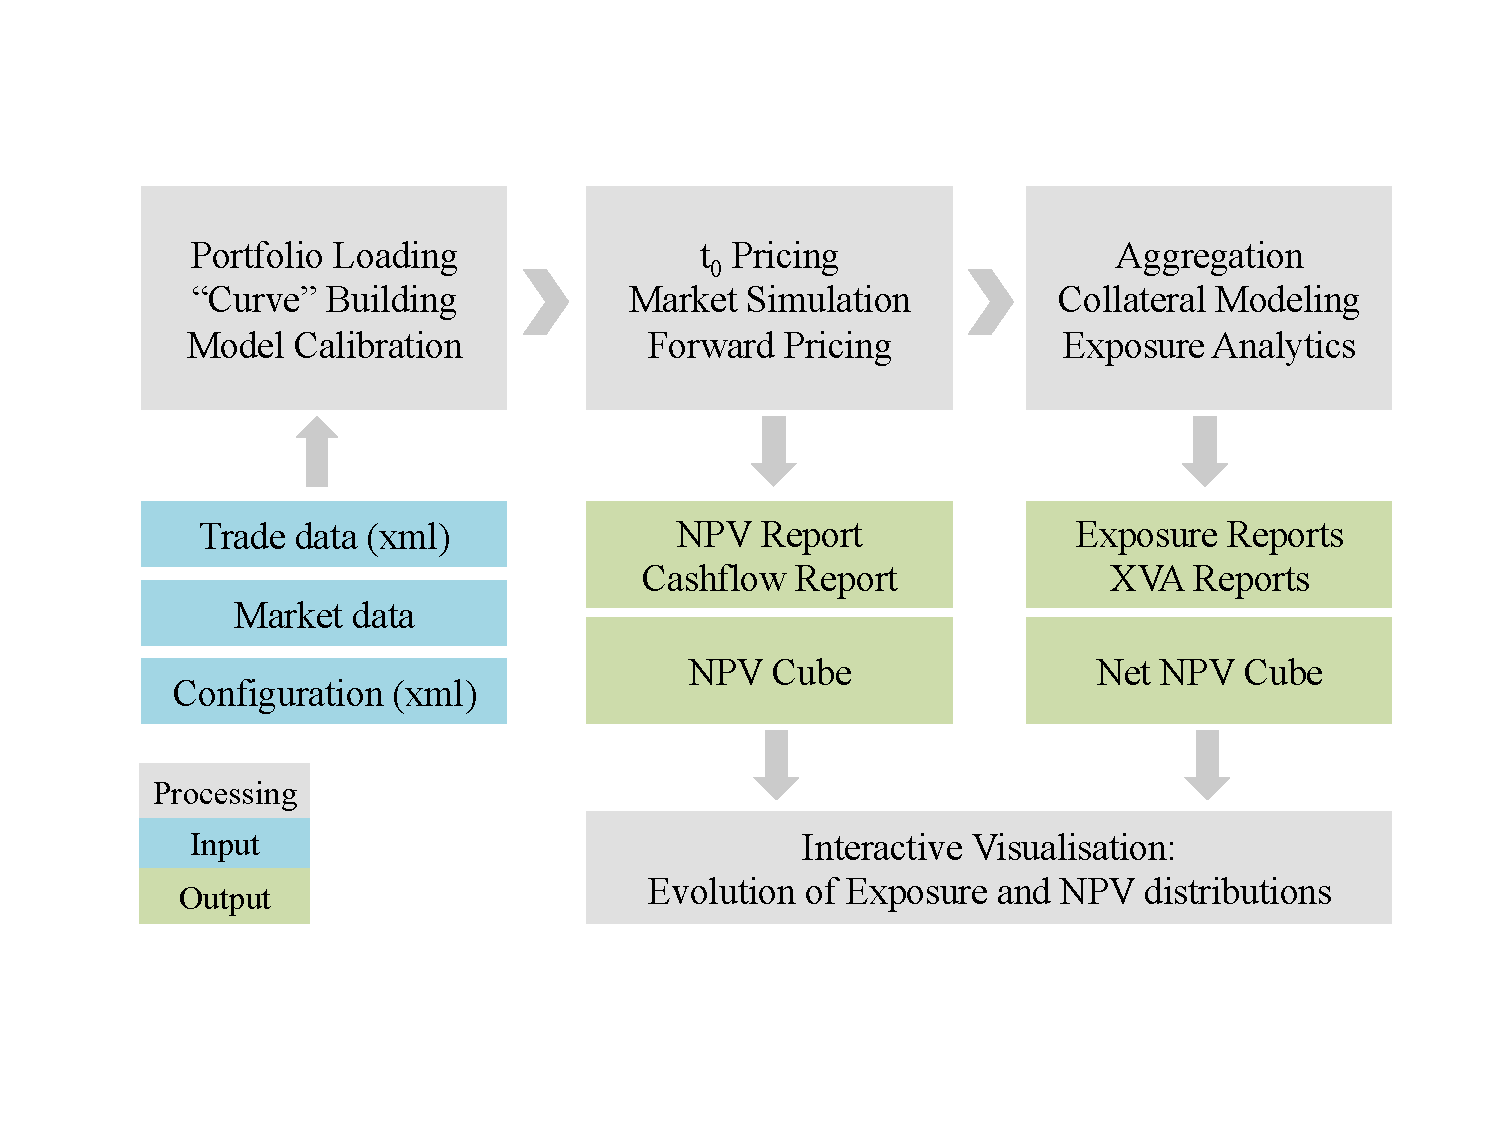
\includegraphics[scale=0.6]{process.pdf}
\end{center}
\caption{Sketch of the ORE process, inputs and outputs. }
\label{fig_process}
\end{figure}

The overall ORE process needs to be parametrised using a set of configuration XML files which is the subject of section
\ref{sec:configuration}. The portfolio is provided in XML format which is explained in detail in sections
\ref{sec:portfolio_data} and \ref{sec:nettingsetinput}. Note that ORE comes with 'Schema' files for all supported
products so that any portfolio xml file can be validated before running through ORE. Market data is provided in a simple
three-column text file with unique human-readable labelling of market data points, as explained in section
\ref{sec:market_data}.  \\

The first processing step (upper left box) then comprises 
\begin{itemize}
\item loading the portfolio to be analysed, 
\item building any yield curves or other 'term structures' needed for pricing, 
\item calibration of pricing and simulation models.
\end{itemize}

The second processing step (upper middle box) is then 
\begin{itemize}
\item portfolio valuation, cash flow generation,
\item going forward - conventional risk analysis such as sensitivity analysis and stress testing, standard-rule capital
  calculations such as SA-CCR, etc,
\item and in particular, more time-consuming, the market simulation and portfolio valuation through time under Monte
  Carlo scenarios.
\end{itemize}
This process step produces several reports (NPV, cashflows etc) and in particular an {\bf NPV cube}, i.e. NPVs per
trade, scenario and future evaluation date. The cube is written to a file in both condensed binary and human-readable
text format.  \\

The third processing step (upper right box) performs more 'sophisticated' risk ana\-ly\-sis by post-processing the NPV
cube data:
\begin{itemize}
\item aggregating over trades per netting set, 
\item applying collateral rules to compute simulated variation margin as well as simulated (dynamic) initial margin
  posting,
\item computing various XVAs including CVA, DVA, FVA, MVA for all netting sets, with and without taking collateral
  (variation and initial margin) into account, on demand with allocation to the trade level.
\end{itemize}
The output of this process step are XVA reports and the 'net' NPV cube, i.e. after aggregation, netting and collateral. \\

The example section \ref{sec:examples} demonstrates for representative product types how the described processing steps
can be combined in a simple batch process which produces the mentioned reports, output files and exposure evolution
graphs in one 'go'.

Moreover, both NPV cubes can be further analysed interactively using a visualisation tool introduced in section
\ref{sec:jupyter}. And finally, sections \ref{sec:calc} and \ref{sec:excel} demonstrate how ORE processes can be
launched in spreadsheets and key results presented automatically within the same sheet.

%========================================================
\section{Getting and Building ORE}\label{sec:installation}
%========================================================

You can get ORE in two ways, either by downloading a release bundle as described in section \ref{sec:release} or by
checking out the source code from the github repository as described in section \ref{sec:build_ore}.

\subsection{ORE Releases}\label{sec:release}

ORE releases are regularly provided in the form of source code archives, Windows exe\-cutables {\tt ore.exe}, example
cases and documentation. Release archives will be provided at \url{https://github.com/opensourcerisk/engine/releases}.

\medskip
The release consists of a single archive in zip format
\begin{itemize}
\item {\tt ORE-<VERSION>.zip}
\end{itemize}

When unpacked, it creates a directory {\tt ORE-<VERSION>} with the following files respectively subdirectories
\begin{enumerate}
%\item {\tt bin/win32/ore.exe}
%\item {\tt bin/x64/ore.exe}
\item {\tt App/}
\item {\tt Docs/}
\item {\tt Examples/}
\item {\tt FrontEnd/}
\item {\tt OREAnalytics/}
\item {\tt OREData/}
\item {\tt QuantExt/}
\item {\tt ThirdPartyLibs/}
\item {\tt tools/}
\item {\tt xsd/}
\item {\tt userguide.pdf}
\end{enumerate} 

The first three items and {\tt userguide.pdf} are sufficient to run the compiled ORE application
on the list of examples described in the user guide (this works on Windows only). The Windows executables are located in {\tt App/bin/Win32/Release/} respectively {\tt App/bin/x64/Release/}. To continue with the compiled
executables:
\begin{itemize}
\item Ensure that the scripting language Python is installed on your computer, see also section \ref{sec:python}
  below;
\item Move on to the examples in section \ref{sec:examples}.
\end{itemize}

\medskip
To build ORE from sources:
\begin{itemize}
\item Set up Boost as described in section \ref{sec:boost}, unless already installed
\item Set up QuantLib 1.11 \cite{QL,quantlib-install} from its github or sourceforge download page, unless already
  installed; QuantLib needs to be located in this project directory {\tt ORE-<VERSION>}. Alternatively, you can create a
  symbolic link named QuantLib here that points to the actual QuantLib directory
\item Build QuantExt, OREData, OREAnalytics, App (in this order) as described in section \ref{sec:build}
\item Note that ThirdPartyLibs does not need to be built, it contains RapdidXml, header only code for reading and
  writing XML files
\item Move on to section \ref{sec:python} and the examples in section \ref{sec:examples}.
\end{itemize}

Open {\tt Docs/html/index.html} to see the API documentation for QuantExt, OREData and OREAnalytics, generated by
doxygen.

\subsection{Building ORE}\label{sec:build_ore}

ORE's source code is hosted on github.com at \url{https://github.com/opensourcerisk/engine} using {\tt git}, a free and
open source distributed version control system.

\subsubsection{Git}

To access the current code base on GitHub, one needs to get {\tt git} installed first.
   
\begin{enumerate}
\item Install and setup Git on your machine following instructions at \cite{git-download}

\item Fetch ORE from github by running the following: 

{\tt\% git clone https://github.com/opensourcerisk/engine.git ore}      

This will create a folder 'ore' in your current directory that contains the codebase.

\item Initially, the QuantLib subdirectory under {\tt ore} is empty as it is a submodule pointing to the official
  QuantLib repository. To pull down locally, use the following commands:

{\tt
\% cd ore \\
\% git submodule init \\
\% git submodule update
}

\end{enumerate}

\subsubsection{Boost}\label{sec:boost}

QuantLib and ORE depend on the boost C++ libraries. Hence these need to be installed before building QuantLib and
ORE. With Unix (Linux, OS X), we recommend boost version 1\_55 or higher, with Windows we recommend boost version 1\_57
or higher. Older versions may work on some platforms and system configurations, but were not tested.

\subsubsection*{Windows}

\begin{enumerate}
\item Download the pre-compiled binaries for MSVC-14 (MSVC2015) from \cite{boost-binaries}
%, any recent version should work
\begin{itemize}
\item 32-bit: \cite{boost-binaries}{\bs}VERSION{\bs}boost\_VERSION-msvc-14.0-32.exe{\bs}download 
\item 64-bit: \cite{boost-binaries}{\bs}VERSION{\bs}boost\_VERSION-msvc-14.0-64.exe{\bs}download
\end{itemize}
\item Start the installation file and choose an installation folder. Take a note of that folder as it will be needed
  later on.
\item Finish the installation by clicking Next a couple of times.
\end{enumerate}
    
Alternatively, compile all Boost libraries directly from the source code:

\begin{enumerate}
\item Open a Visual Studio Tools Command Prompt
\begin{itemize}
\item 32-bit: VS2015/VS2013 x86 Native Tools Command Prompt
\item 64-bit: VS2015/VS2013 x64 Native Tools Command Prompt
\end{itemize}
\item Navigate to the boost root directory
\item Run bootstrap.bat
\item Build the libraries from the source code
\begin{itemize}
\item 32-bit: \\
  {\footnotesize\tt .{\bs}b2 --stagedir=.{\bs}lib{\bs}Win32{\bs}lib --build-type=complete toolset=msvc-14.0 \bs \\
    address-model=32 --with-test --with-system --with-filesystem  \bs \\
    --with-serialization --with-regex --with-date\_time stage}
\item 64-bit: \\
  {\footnotesize\tt .{\bs}b2 --stagedir=.{\bs}lib{\bs}x64{\bs}lib --build-type=complete toolset=msvc-14.0 \bs \\
    address-model=64 --with-test --with-system --with-filesystem \bs \\
    --with-serialization --with-regex --with-date\_time stage}
\end{itemize}
\end{enumerate}

\subsubsection*{Unix}

\begin{enumerate}
\item Download Boost from \cite{boost} and build following the instructions on the site
%, any recent version should work
\item Define the environment variable BOOST that points to the boost directory
(so includes should be in BOOST and libs should be in BOOST/stage/lib)
\end{enumerate}

\subsubsection{ORE Libraries and Application}\label{sec:build}

\subsubsection*{Windows}

\begin{enumerate}

\item Download and install Visual Studio Community Edition (Version 2013 or later). 
During the installation, make sure you install the Visual
C++ support under the Programming Languages features (disabled by default).

\item To configure the boost paths in Visual Studio open any of the Visual Studio solution files in item 3 below and
  select View $\rightarrow$ Other Windows $\rightarrow$ Property Manager. It does not matter which solution you open, if
  it is for example the Quant\-Ext solution you should see two Projects 'QuantExt' and 'quantexttestsuite' in the property
  manager. Expand any of them (e.g. QuantExt) and then one of the Win32 or x64 configurations. The settings will be
  specific for the Win32 or x64 configuration but otherwise it does not matter which of the projects or configurations
  you expand, they all contain the same configuration file. You should now see 'Microsoft.Cpp.Win32.user' respectively
  'Microsoft.Cpp.x64.user' depending on whether you chose a Win32 or a x64 configuration. Click on this file to open the
  property pages. Select VC++ Directories and then add your boost directory to the 'Include Directories' entry. Likewise
  add your boost library directory to the 'Library Directories' entry. If for example your boost installation is in {\tt
    C:{\bs}boost\_1\_57\_0} and the libraries reside in the {\tt stage{\bs}lib} subfolder, add {\tt
    C:{\bs}boost\_1\_57\_0} to the 'Include Directories' entry and {\tt C:{\bs}boost\_1\_57\_0{\bs}stage{\bs} lib} to the
  'Library Directories' entry. Press OK. 
  (Alternatively, create and use an environment variable {\tt \%BOOST\%} pointing to your directory {\tt C:{\bs}boost\_1\_57\_0} instead of the directory itself.) 
  If you want to configure the boost paths for Win32 resp. x64 as well, repeat
  the previous step for 'Microsoft.Cpp. Win32.user' respectively 'Microsoft.Cpp.x64.user'. To complete the configuration
  just close the property manager window.

  % \item Open any solution file and update path to Boost as described in sections 5 \& 6 in
  %   \cite{quantlib-install}. You only need to do this for a single project as this will update the path to boost
  %   across all projects and solutions on your machine. The paths should be set as follow (in case you compiled Boost
  %   on your own, use the path specified using the --stagedir cmd argument):
%
%\begin{itemize}
%\item Include Directories: [Boost Installation Folder]
%\item Library Directories: [Boost Installation Folder]{\bs}libs
%\end{itemize}
%
%\item Add the additional path to the Boost pre-compiled libraries to the linker setting:
%
%\begin{itemize}
%\item 32-bit: [Boost Installation Folder]{\bs}lib32-msvc-14.0
%\item 64-bit: [Boost Installation Folder]{\bs}lib64-msvc-14.0
%\end{itemize}

\item Open each of the sub-projects and compile them in the following order: QuantLib, QuantExt, OREData, OREAnalytics
  and App. For each project, do the following:

\begin{itemize}
\item Switch to the correct platform (i.e. Win32 or x64) from the Configuration Manager. The selection should match the
  pre-compiled version of Boost. Trying to compile using a mixed configuration (e.g. Boost 64-bit and 32-bit QuantLib)
  will fail.
\item Compile the project: Build $\rightarrow$ Build Solution
\item Once the compilation is complete, run the test suite.
\end{itemize}

\end{enumerate}

\subsubsection*{Unix}

\begin{enumerate}

\item Build QuantLib as usual.

{\tt\footnotesize
\% cd QuantLib \\
\% ./autogen.sh \\
\% ./configure --with-boost-include=\$BOOST --with-boost-lib=\$BOOST/stage/lib \\
\% make -j4 
}

\item Build QuantExt

{\tt\footnotesize
\% cd QuantExt \\
\% ./autogen.sh \\
\% ./configure \\
\% make -j4
}

This will build both the QuantExt library and test suite.

\item Run the test suite

{\tt\footnotesize
\% ./test/quantext-test-suite 
}

\item  Build OREData, OREAnalytics and their test suites. 

Follow the same steps as for QuantExt.
To run the unit test suites, do 

{\tt\footnotesize
\% ./test/ored-test-suite 
}

and 

{\tt\footnotesize
\% ./test/orea-test-suite 
}

in the respective library directories.

\item Build App/ore

{\tt\footnotesize
\% cd App \\
\% ./autogen.sh \\
\% ./configure \\
\% make -j4
}

Note: On Linux systems, the 'locale' settings can negatively affect the ORE process and output. To avoid this, we
recommend setting the environment variable {\tt LC\_NUMERIC} to {\tt C}, e.g. in a bash shell, do

{\tt\footnotesize
\% export LC\_NUMERIC=C
}

before running ORE or any of the examples below. This will suppress thousand separators in numbers when converted to
strings.

\item Run Examples (see section \ref{sec:examples})

{\tt\footnotesize
\% cd Examples/Example\_1 \\
\% python run.py 
}

\end{enumerate}

\subsection{Python and Jupyter}\label{sec:python}

Python (version 3.5 or higher) is required to run the examples in section \ref{sec:examples} and plot exposure
evolutions. Moreover, we use Jupyter \cite{jupyter} in section \ref{sec:visualisation} to visualise simulation
results. Both are part of the 'Anaconda Open Data Science Analytics Platform' \cite{Anaconda}. Anaconda installation
instructions for Windows, OS X and Linux are available on the Anaconda site, with graphical installers for
Windows\footnote{With Windows, after a fresh installation of Python the user may have to run the {\tt python} command
  once in a command shell so that the Python executable will be found subsequently when running the example scripts in
  section \ref{sec:examples}.}, Linux and OS X.

With Linux and OS X, the following environment variable settings are required
\begin{itemize}
\item set {\tt LANG} and {\tt LC\_ALL } to {\tt en\_US.UTF-8} or {\tt en\_GB.UTF-8}
\item set {\tt LC\_NUMERIC} to {\tt C}. 
\end{itemize}
The former is required for both running the Python scripts in the examples section, as well as successful installation
of the following packages. \\

The full functionality of the Jupyter notebook introduced in section \ref{sec:jupyter} requires furthermore installing
\begin{itemize}
\item jupyter\_dashboards: \url{https://github.com/jupyter-incubator/dashboards}
\item ipywidgets: \url{https://github.com/ipython/ipywidgets}
\item pythreejs: \url{https://github.com/jovyan/pythreejs}
\item bqplot: \url{https://github.com/bloomberg/bqplot}
\end{itemize}
With Python and Anaconda already installed, this can be done by running these commands
\begin{itemize}
\item {\tt conda install -c conda-forge ipywidgets}
\item {\tt pip install jupyter\_dashboards}
\item {\tt jupyter dashboards quick-setup --sys-prefix}
\item {\tt conda install -c conda-forge bqplot}
\item {\tt conda install -c conda-forge pythreejs}
\end{itemize}
Note that the bqplot installation requires the environment settings mentioned above.

%========================================================
\section{Examples}\label{sec:examples}
%========================================================

The examples shown in table \ref{tab_0} are intended to help with getting started with ORE, and to serve as plausibility
checks for the simulation results generated with ORE.

\begin{table}[hbt]
\scriptsize
\begin{center}
\begin{tabular}{|c|l|}
\hline
Example & Description \\
\hline
\hline
1 & Vanilla at-the-money Swap with flat yield curve \\
\hline
2 & Vanilla Swap with normal yield curve \\
\hline
3 & European Swaption \\
\hline
4 & Bermudan Swaption \\
\hline
5 & Callable Swap \\
\hline
6 & Cap/Floor \\
\hline
7 & FX Forward \\
  & European FX Option \\ 
\hline
8 & Cross Currency Swap without notional reset \\
\hline
9 & Cross Currency Swap with notional reset \\
\hline
10 & Three-Swap portfolio with netting and collateral \\
   & XVAs - CVA, DVA, FVA, MVA, COLVA \\
   & Exposure and XVA Allocation to trade level \\
\hline
11 & Basel exposure measures - EE, EPE, EEPE \\
\hline
12 & Long term simulation with horizon shift \\
\hline
13 & Dynamic Initial Margin and MVA \\
\hline
14 & Minimal Market Data Setup \\
\hline
15 & Sensitivity Analysis and Stress Testing \\
\hline
16 & Equity Derivatives Exposure \\
\hline
17 & Inflation Swaps \\
\hline
18 & Bonds and Amortisation Structures\\
\hline
19 & Swaption Pricing with Smile\\
\hline
20 & Credit Default Swap Pricing\\
\hline
21 & Constant Maturity Swap Pricing\\
\hline
22 & Option Sensitivity Analysis with Smile\\
\hline
23 & Forward Rate Agreement and Averaging OIS Exposure\\
\hline
\end{tabular}
\caption{ORE examples.}
\label{tab_0}
\end{center}
\end{table}

\todo[inline]{Revise examples overview table when examples are complete, inflation is done}
All example results can be produced with the Python scripts {\tt run.py} in the ORE release's {\tt Examples/Example\_\#}
folders which work on both Windows and Unix platforms. In a nutshell, all scripts call ORE's command line application
with a single input XML file

\medskip
\centerline{\tt ore[.exe] ore.xml}
\medskip

They produce a number of standard reports and exposure graphs in PDF format. The structure of the input file and of the
portfolio, market and other configuration files referred to therein will be explained in section
\ref{sec:configuration}.

\medskip ORE is driven by a number of input files, listed in table \ref{tab_1} and explained in detail in sections
\ref{sec:configuration} to \ref{sec:fixings}. In all examples, these input files are either located in the example's sub
directory {\tt Examples/Example\_\#/Input} or the main input directory {\tt Examples/Input} if used across several
examples. The particular selection of input files is determined by the 'master' input file {\tt ore.xml}.

\begin{table}[h]
\scriptsize
\begin{center}
\begin{tabular}{|l|p{11cm}|}
  \hline
  File Name & Description \\
  \hline
  {\tt ore.xml}&   Master input file, selection of further inputs below and selection of analytics \\
  {\tt portfolio.xml} & Trade data \\
  {\tt netting.xml} &  Collateral (CSA) data \\
  {\tt simulation.xml} & Configuration of simulation model and market\\
  {\tt market.txt} &  Market data snapshot \\
  {\tt fixings.txt} &  Index fixing history \\
  {\tt curveconfig.xml} & Curve and term structure composition from individual market instruments\\
  {\tt conventions.xml} & Market conventions for all market data points\\
  {\tt todaysmarket.xml} &  Configuration of the market composition, relevant for the pricing of the given portfolio as
                           of today (yield curves, FX rates, volatility surfaces etc) \\
  {\tt pricingengines.xml} &  Configuration of pricing methods by product\\
  \hline
\end{tabular}
\end{center}
\caption{ORE input files}
\label{tab_1}
\end{table}

The typical list of output files and reports is shown in table \ref{tab_2}. The names of output files can be configured
through the master input file {\tt ore.xml}. Whether these reports are generated also depends on the setting in {\tt
  ore.xml}. For the examples, all output will be written to the directory {\tt Examples/Example\_\#/Output}.

\begin{table}[h]
\scriptsize
\begin{center}
\begin{tabular}{|l|p{11cm}|}
\hline
File Name & Description \\
\hline
{\tt npv.csv}&   NPV report \\
{\tt flows.csv} & Cashflow report \\
{\tt curves.csv} & Generated yield (discount) curves report \\
{\tt xva.csv} & XVA report, value adjustments at netting set and trade level \\
{\tt exposure\_trade\_*.csv} & Trade exposure evolution reports\\
{\tt exposure\_nettingset\_*.csv} &  Netting set exposure evolution reports\\
{\tt rawcube.csv} & NPV cube in readable text format \\
{\tt netcube.csv} & NPV cube after netting and colateral, in readable text format \\
{\tt *.dat} & Intermediate storage of NPV cube and scenario data in binary format \\
{\tt *.pdf} &  Exposure graphics produced by the python script {\tt run.py} after ORE completed\\
\hline
\end{tabular}
\end{center}
\caption{ORE output files}
\label{tab_2}
\end{table}

Note: When building ORE from sources on Windows platforms, make sure that you copy your {\tt ore.exe} to the binary
directory {\tt bin/win32/} respectively {\tt bin/x64/}. Otherwise the examples may be run using the pre-compiled
executables which come with the ORE release.

%--------------------------------------------------------
\subsection{Interest Rate Swap Exposure}\label{sec:example1}
%--------------------------------------------------------

We start with a vanilla single currency Swap (currency EUR, maturity 20y, notional 10m, receive fixed 2\% annual, pay
6M-Euribor flat). The market yield curves (for both discounting and forward projection) are set to be flat at 2\% for
all maturities, i.e. the Swap is at the money initially and remains at the money on average throughout its life. Running
ORE in directory {\tt Examples/Example\_1} with

\medskip
\centerline{\tt python run.py } 
\medskip

yields the exposure evolution in 

\medskip
\centerline{\tt Examples/Example\_1/Output/*.pdf } 
\medskip

and shown in figure \ref{fig_1}. 
\begin{figure}[h!]
\begin{center}
%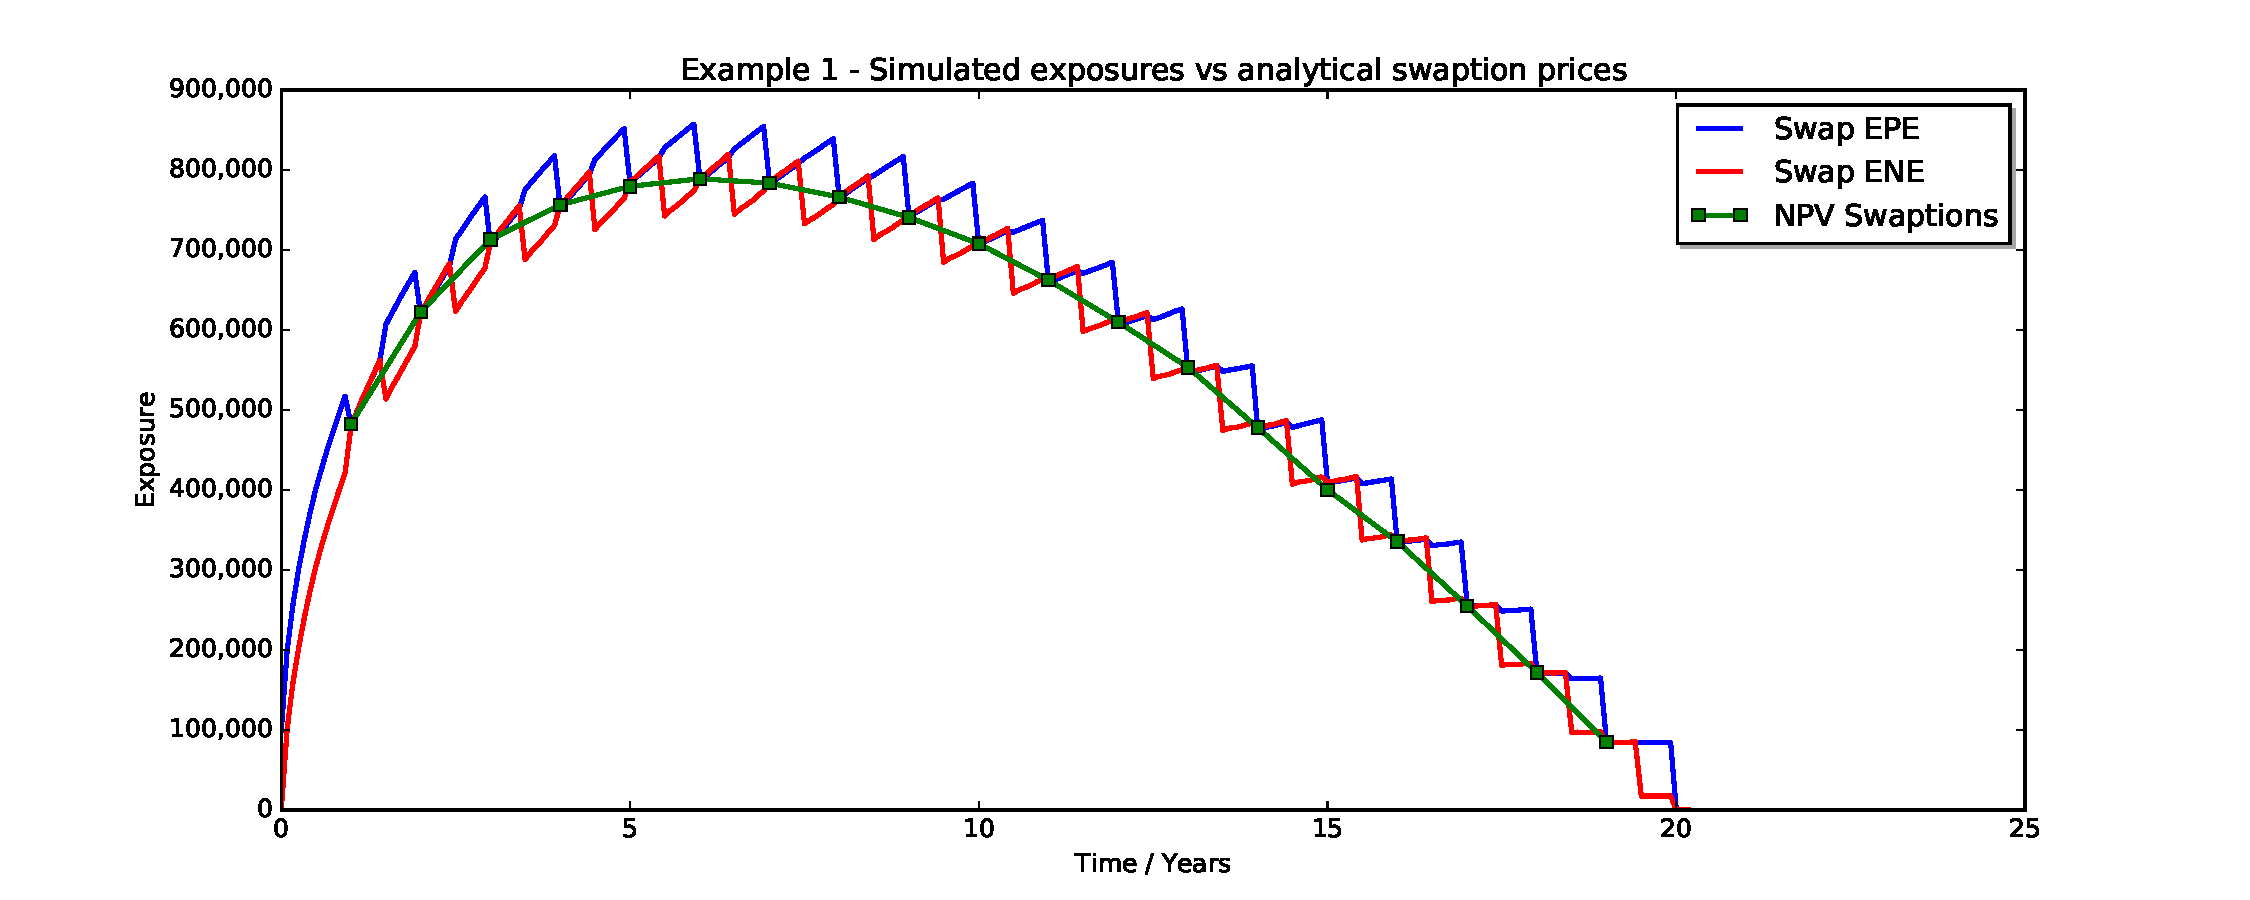
\includegraphics[scale=0.45]{mpl_swap_1_1m_sbb_100k.pdf}
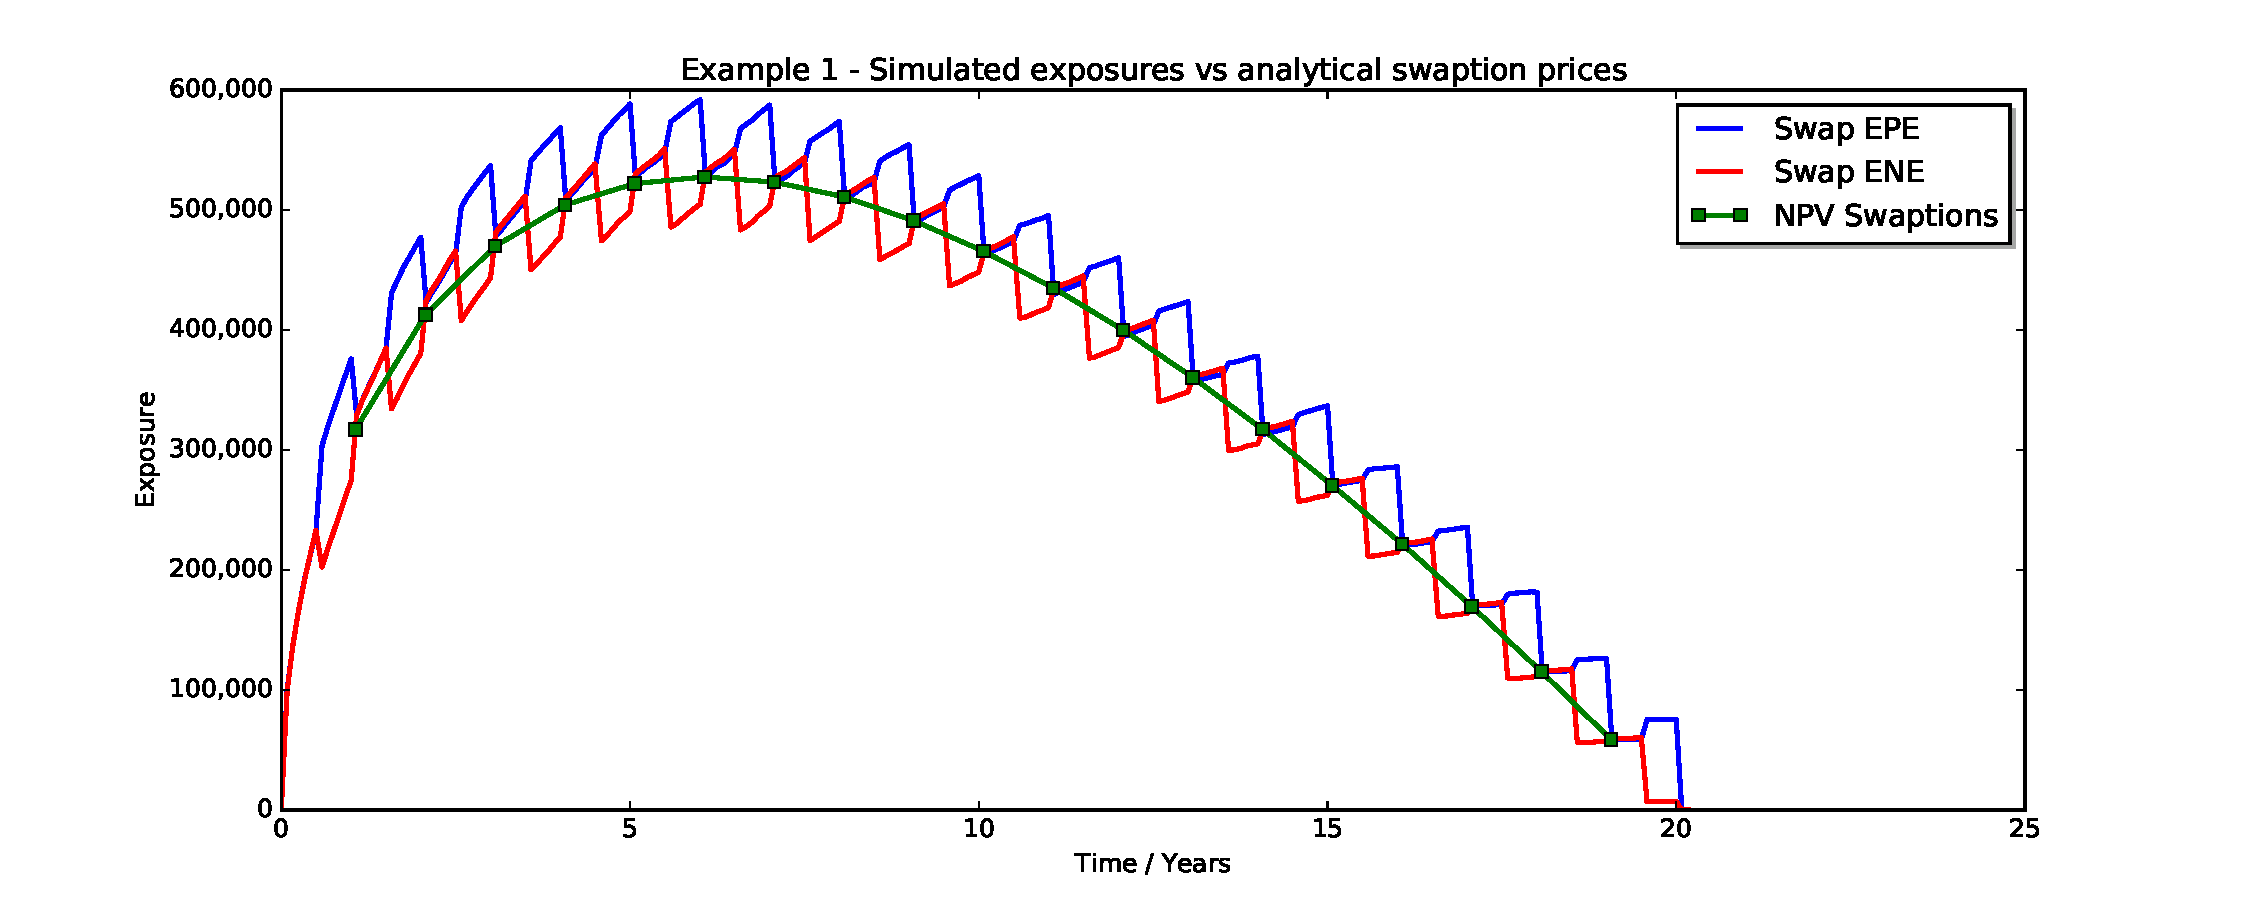
\includegraphics[scale=0.45]{mpl_swap_1_1m_sbb_10k_flat.pdf}
\end{center}
\caption{Vanilla ATM Swap expected exposure in a flat market environment from both parties' perspectives. The symbols are European Swaption prices. The simulation was run with monthly time steps and 10,000 Monte Carlo samples to demonstrate the convergence of EPE and ENE profiles. A similar
outcome can be obtained more quickly with 5,000 samples on a quarterly time grid which is the default setting of Example\_1. }
\label{fig_1}
\end{figure}
Both Swap simulation and Swaption pricing are run with calls to the ORE executable, essentially 

\medskip
\centerline{\tt ore[.exe] ore.xml} 

\centerline{\tt ore[.exe] ore\_swaption.xml} 
\medskip

which are wrapped into the script {\tt Examples/Example\_1/run.py} provided with the ORE release.
It is instructive to look into the input folder in Examples/Example\_1, the content of the main input file {\tt
  ore.xml}, together with the explanations in section \ref{sec:configuration}. \\

This simple example is an important test case which is also run similarly in one of the unit test suites of ORE. The
expected exposure can be seen as a European option on the underlying netting set, see also appendix
\ref{sec:app_exposure}. In this exampl«e, the expected exposure at some future point in time, say 10 years, is equal to
the European Swaption price for an option with expiry in 10 years, underlying Swap start in 10 years and underlying Swap
maturity in 20 years. We can easily compute such standard European Swaption prices for all future points in time where
both Swap legs reset, i.e. annually in this case\footnote{Using closed form expressions for standard European Swaption
  prices.}. And if the simulation model has been calibrated to the points on the Swaption surface which are used for
European Swaption pricing, then we can expect to see that the simulated exposure matches Swaption prices at these annual
points, as in figure \ref{fig_1}.  In Example\_1 we used co-terminal ATM Swaptions for both model calibration and
Swaption pricing. Moreover, as the the yield curve is flat in this example, the exposures from both parties'
perspectives (EPE and ENE) match not only at the annual resets, but also for the period between annual reset of both
legs to the point in time when the floating leg resets. Thereafter, between floating leg (only) reset and next joint
fixed/floating leg reset, we see and expect a deviation of the two exposure profiles.

\medskip Moving to {\tt Examples/Example\_2}, we see what changes when using a realistic (non-flat) market
environment. Running the example with

\medskip
\centerline{\tt python run.py } 
\medskip

yields the exposure evolution in 

\medskip
\centerline{\tt Examples/Example\_2/Output/*.pdf } 
\medskip

shown in figure \ref{fig_2}.
\begin{figure}[h!]
\begin{center}
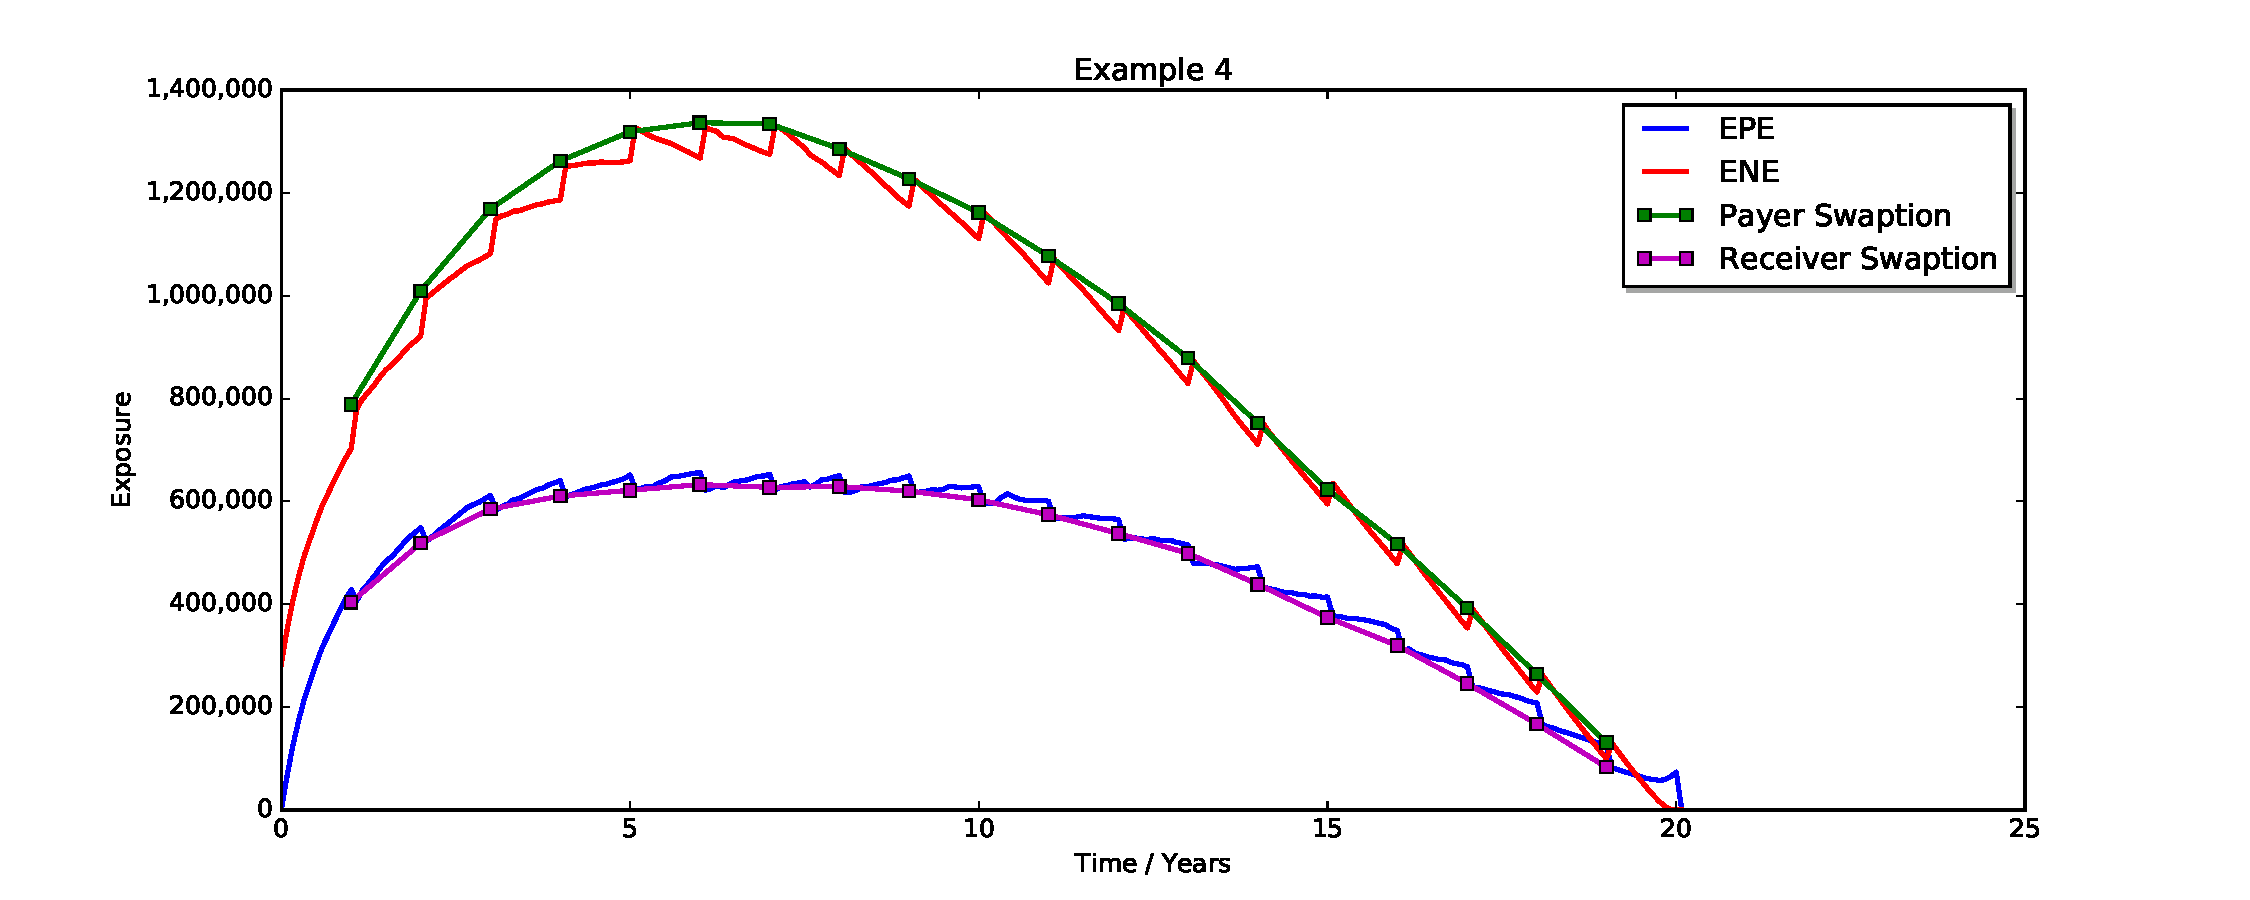
\includegraphics[scale=0.45]{mpl_swap_3.pdf}
\end{center}
\caption{Vanilla ATM Swap expected exposure in a realistic market environment as of 05/02/2016 from both parties'
  perspectives. The Swap is the same as in figure \ref{fig_1} but receiving fixed 1\%, roughly at the money. The symbols
  are the prices of European payer and receiver Swaptions. Simulation with 5000 paths and monthly time steps.}
\label{fig_2}
\end{figure}
In this case, where the curves (discount and forward) are upward sloping, the receiver Swap is at the money at inception
only and moves (on average) out of the money during its life. Similarly, the Swap moves into the money from the
counterparty's perspective. Hence the expected exposure evolutions from our perspective (EPE) and the counterparty's
perspective (ENE) 'detach' here, while both can still be be reconciled with payer or respectively receiver Swaption
prices.

%--------------------------------------------------------
\subsection{European Swaption Exposure}\label{sec:european_swaption}
%--------------------------------------------------------

This demo case in folder {\tt Examples/Example\_3} shows the exposure evolution of European Swaptions with cash and
physical delivery, respectively, see figure \ref{fig_3}.
\begin{figure}[h!]
\begin{center}
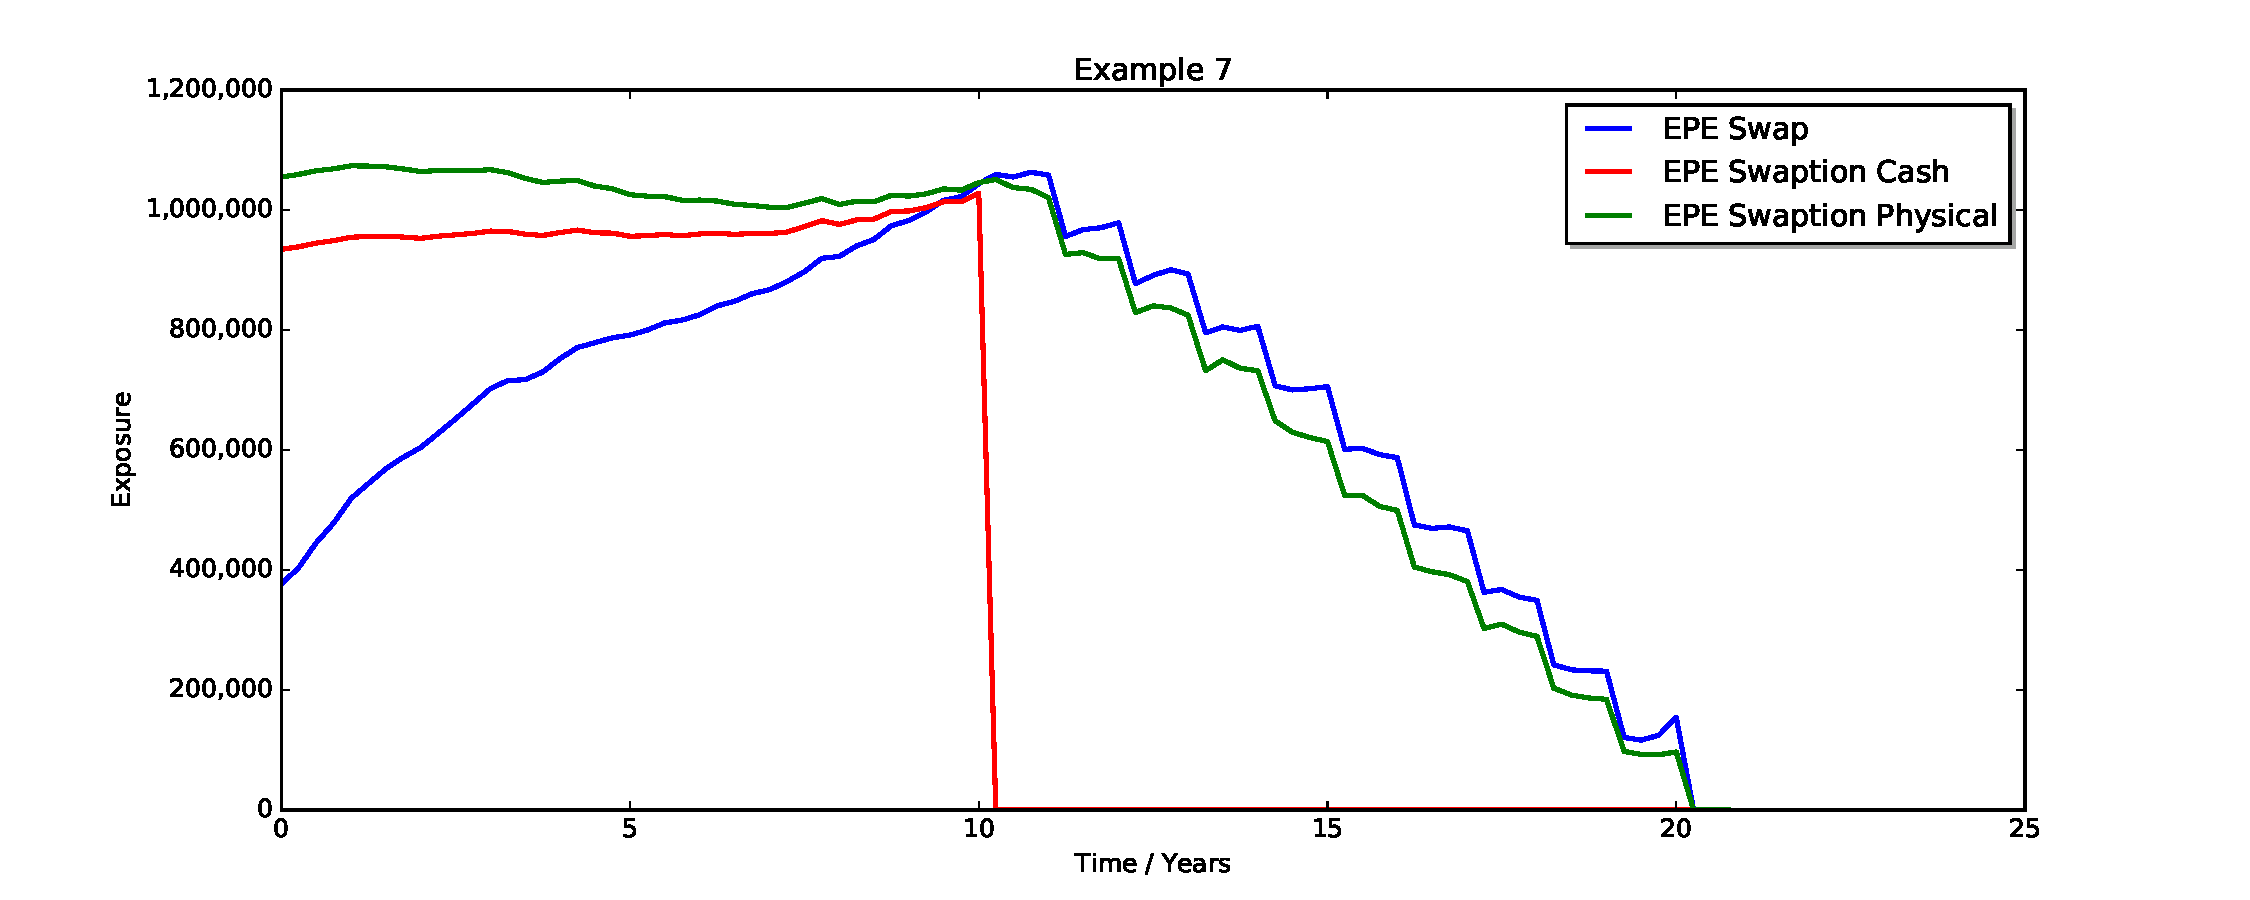
\includegraphics[scale=0.45]{mpl_swaption.pdf}
\end{center}
\caption{European Swaption exposure evolution, expiry in 10 years, final maturity in 20 years, for cash and physical
  delivery. Simulation with 1000 paths and quarterly time steps.}
\label{fig_3}
\end{figure}
The delivery type (cash vs physical) yields significantly different valuations as of today due to the steepness of the
relevant yield curves (EUR). The cash settled Swaption's exposure graph is truncated at the exercise date, whereas the
physically settled Swaption exposure turns into a Swap-like exposure after expiry. For comparison, the example also
provides the exposure evolution of the underlying forward starting Swap which yields a somewhat higher exposure after
the forward start date than the physically settled Swaption. This is due to scenarios with negative Swap NPV at expiry
(hence not exercised) and positive NPVs thereafter.

%--------------------------------------------------------
\subsection{Bermudan Swaption Exposure}
%--------------------------------------------------------

This demo case in folder {\tt Examples/Example\_4} shows the exposure evolution of Bermudan rather than European
Swaptions with cash and physical delivery, respectively, see figure \ref{fig_3b}.
\begin{figure}[h!]
\begin{center}
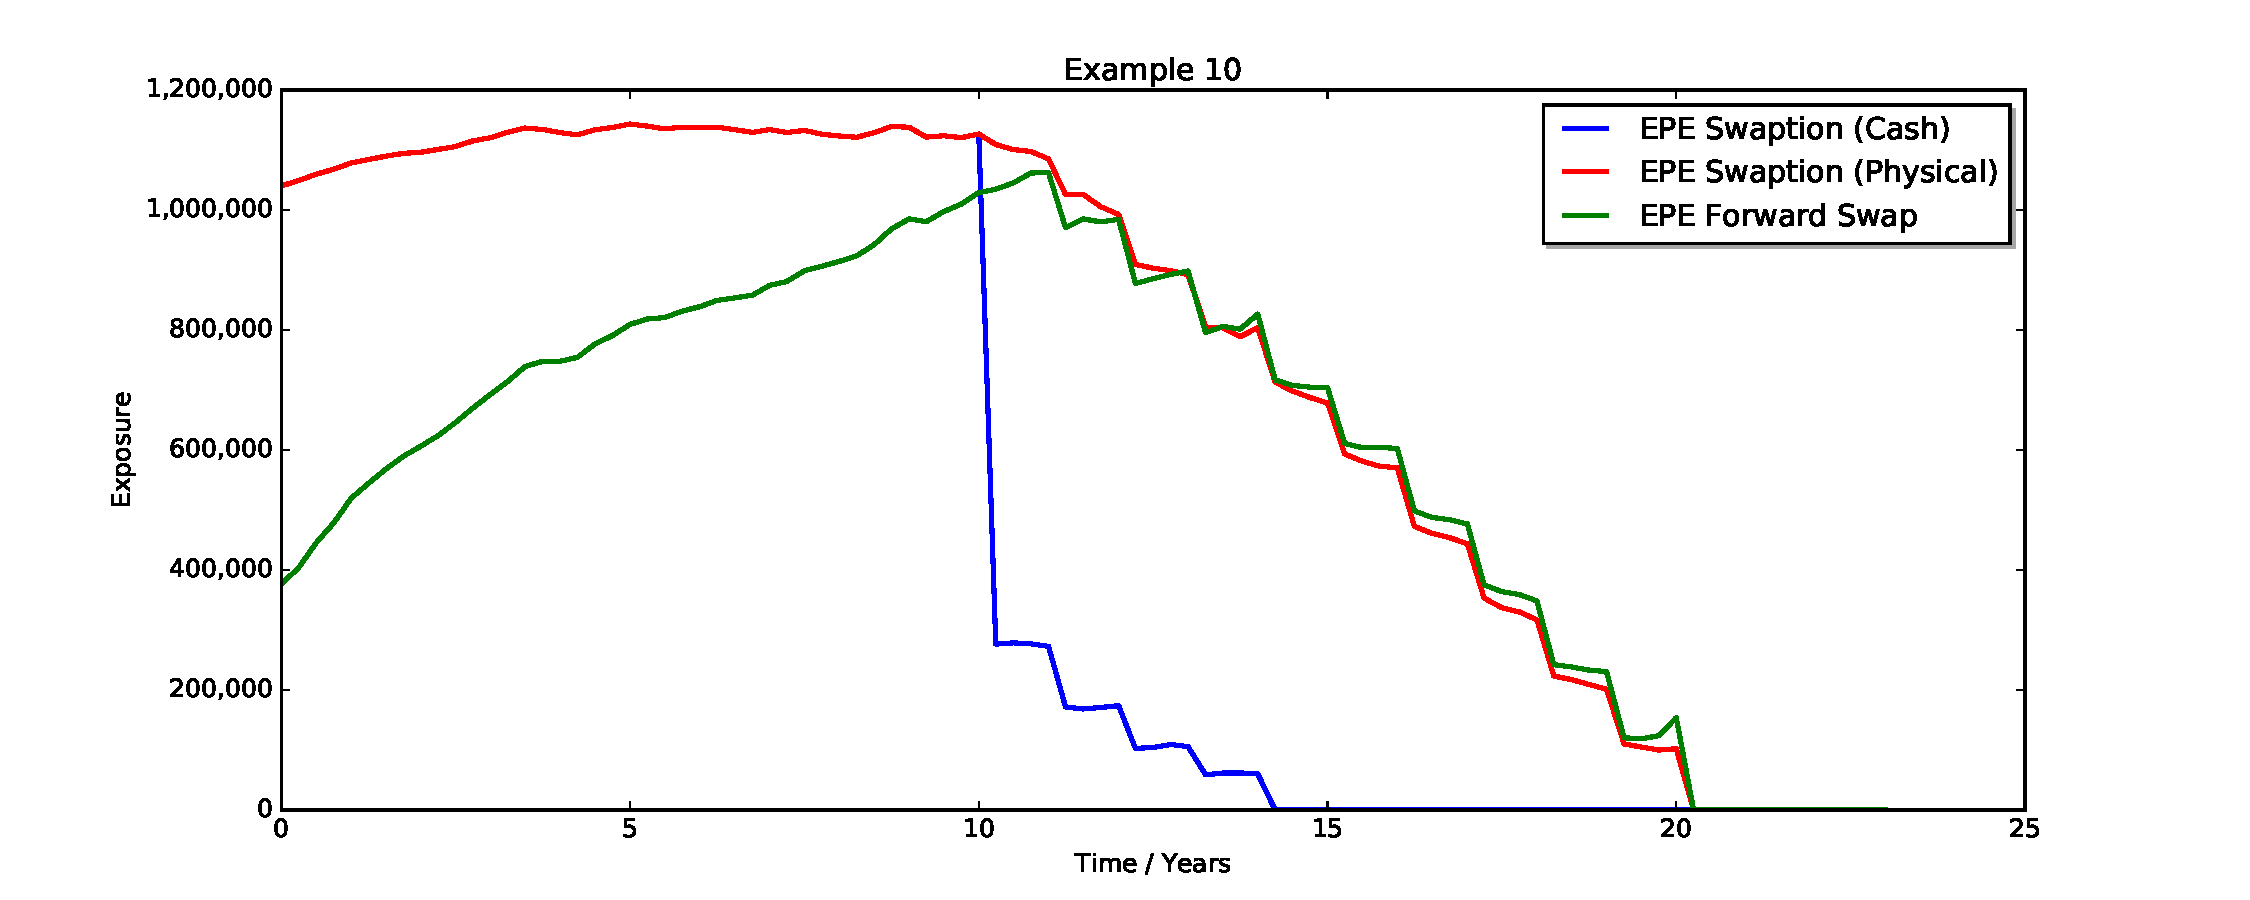
\includegraphics[scale=0.45]{mpl_bermudan_swaption.pdf}
\end{center}
\caption{Bermudan Swaption exposure evolution, 5 annual exercise dates starting in 10 years, final maturity in 20 years,
  for cash and physical delivery. Simulation with 1000 paths and quarterly time steps.}
\label{fig_3b}
\end{figure}
The underlying Swap is the same as in the European Swaption example in section \ref{sec:european_swaption}. Note in
particular the difference between the Bermudan and European Swaption exposures with cash settlement: The Bermudan shows
the typical step-wise decrease due to the series of exercise dates. Also note that we are using the same Bermudan option
pricing engines for both settlement types, in contrast to the European case, so that the Bermudan option cash and
physical exposures are identical up to the first exercise date. When running this example, you will notice the
significant difference in computation time compared to the European case (ballpark 30 minutes here for 2 Swaptions, 1000
samples, 90 time steps). The Bermudan example takes significantly more computation time because we use an LGM grid
engine for pricing under scenarios in this case. In a realistic context one would more likely resort to American Monte
Carlo simulation, feasible in ORE, but not provided in the current release. However, this implementation can be used to
benchmark any faster / more sophisticated approach to Bermudan Swaption exposure simulation.

%--------------------------------------------------------
\subsection{Callable Swap Exposure}
%--------------------------------------------------------

This demo case in folder {\tt Examples/Example\_5} shows the exposure evolution of a European callable Swap, represented
as two trades - the non-callable Swap and a Swaption with physical delivery. We have sold the call option, i.e. the
Swaption is a right for the counterparty to enter into an offsetting Swap which economically terminates all future flows
if exercised. The resulting exposure evolutions for the individual components (Swap, Swaption), as well as the callable
Swap are shown in figure \ref{fig_4}.
\begin{figure}[h!]
\begin{center}
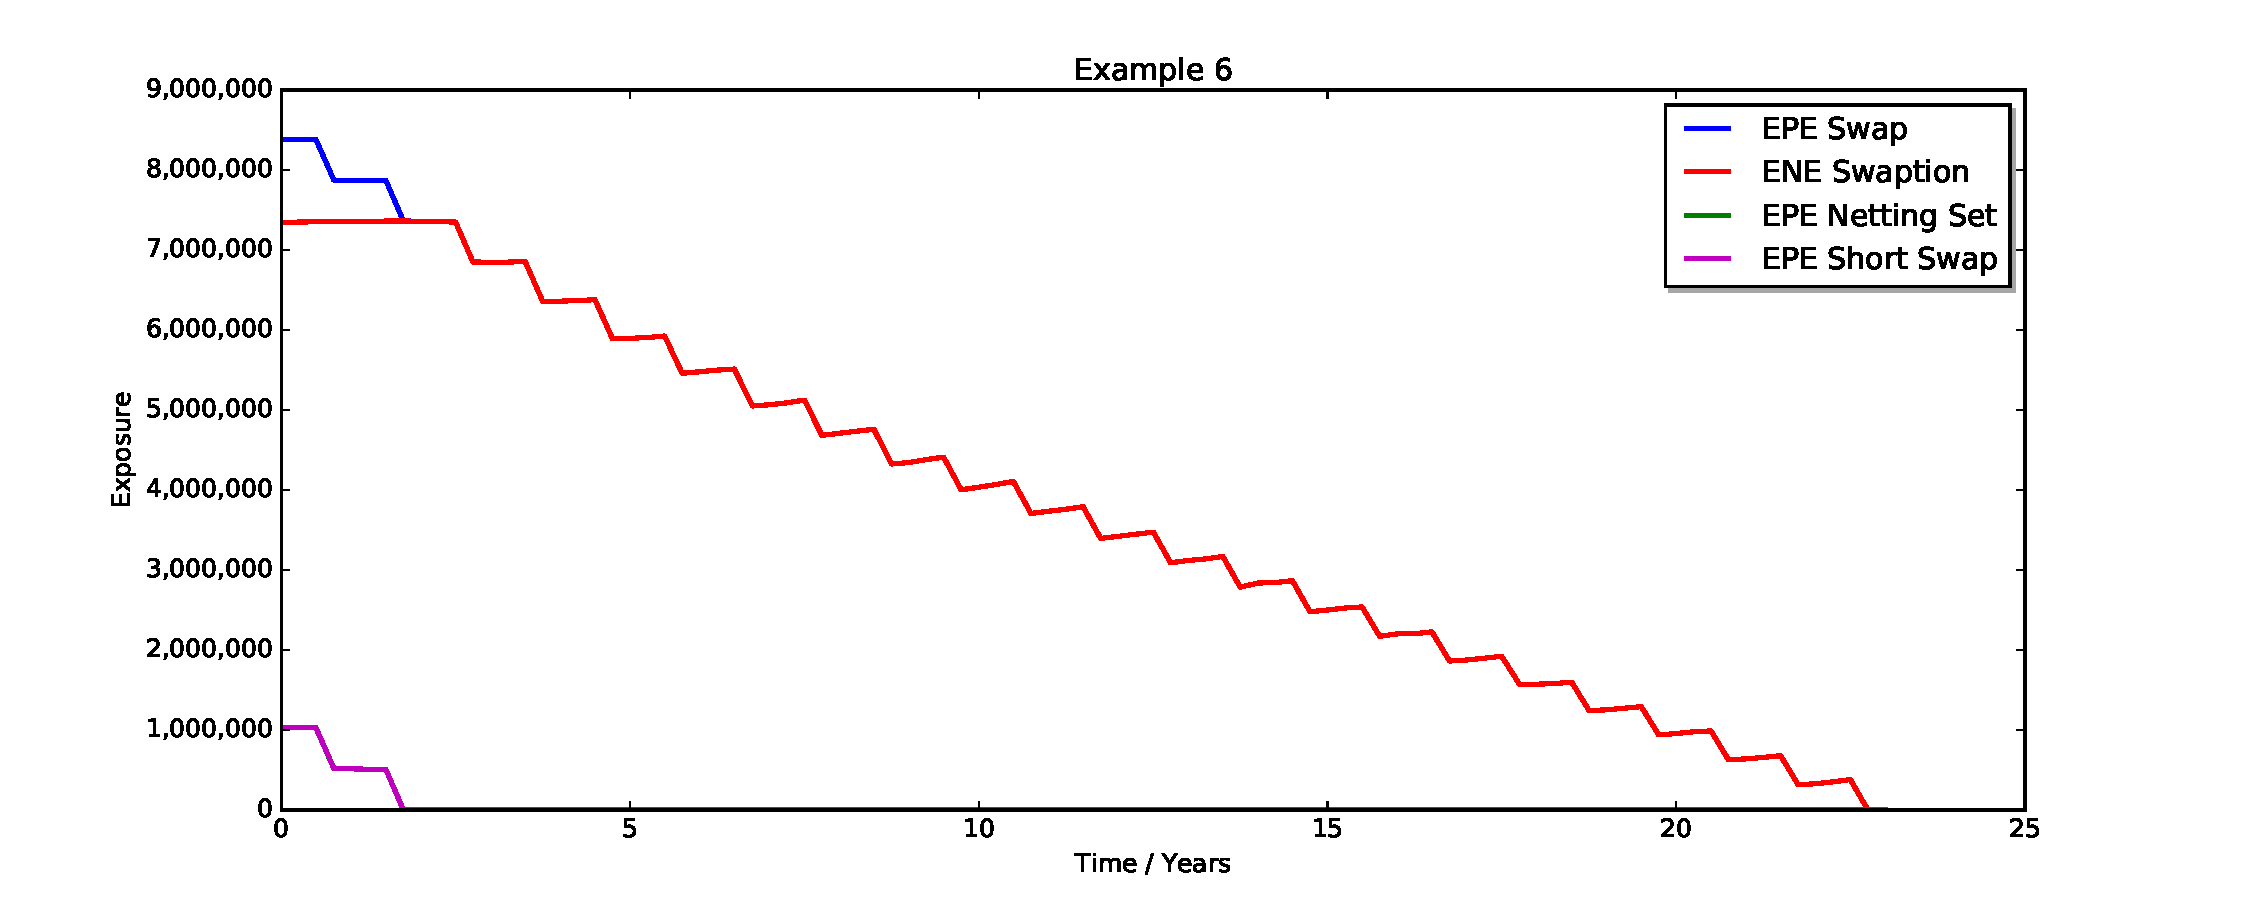
\includegraphics[scale=0.45]{mpl_callable_swap.pdf}
\end{center}
\caption{European callable Swap represented as a package consisiting of non-callable Swap and Swaption. The Swaption has
  physical delivery and offsets all future Swap cash flows if exercised. The exposure evolution of the package is shown
  here as 'EPE NettingSet' (green line). This is covered by the pink line, the exposure evolution of the same Swap but
  with maturity on the exercise date. The graphs match perfectly here, because the example Swap is deep in the money and
  exercise probability is close to one. Simulation with 5000 paths and quarterly time steps.}
\label{fig_4}
\end{figure}
The example is an extreme case where the underlying Swap is deeply in the money (receiving fixed 5\%), and hence the
call exercise probability is close to one. Modify the Swap and Swaption fixed rates closer to the money ($\approx$ 1\%)
to see the deviation between net exposure of the callable Swap and the exposure of a 'short' Swap with maturity on
exercise.

%--------------------------------------------------------
\subsection{Cap/Floor Exposure}\label{sec:capfloor}
%--------------------------------------------------------

The example in folder {\tt Examples/Example\_6} generates exposure evolutions of several Swaps, caps and floors. The
example shown in figure \ref{fig_capfloor_1} ('portfolio 1') consists of a 20y Swap receiving 3\% fixed and paying
Euribor 6M plus a long 20y Collar
with both cap and floor at 4\% so that the net exposure corresponds to a Swap paying 1\% fixed. \\

\begin{figure}[h!]
\begin{center}
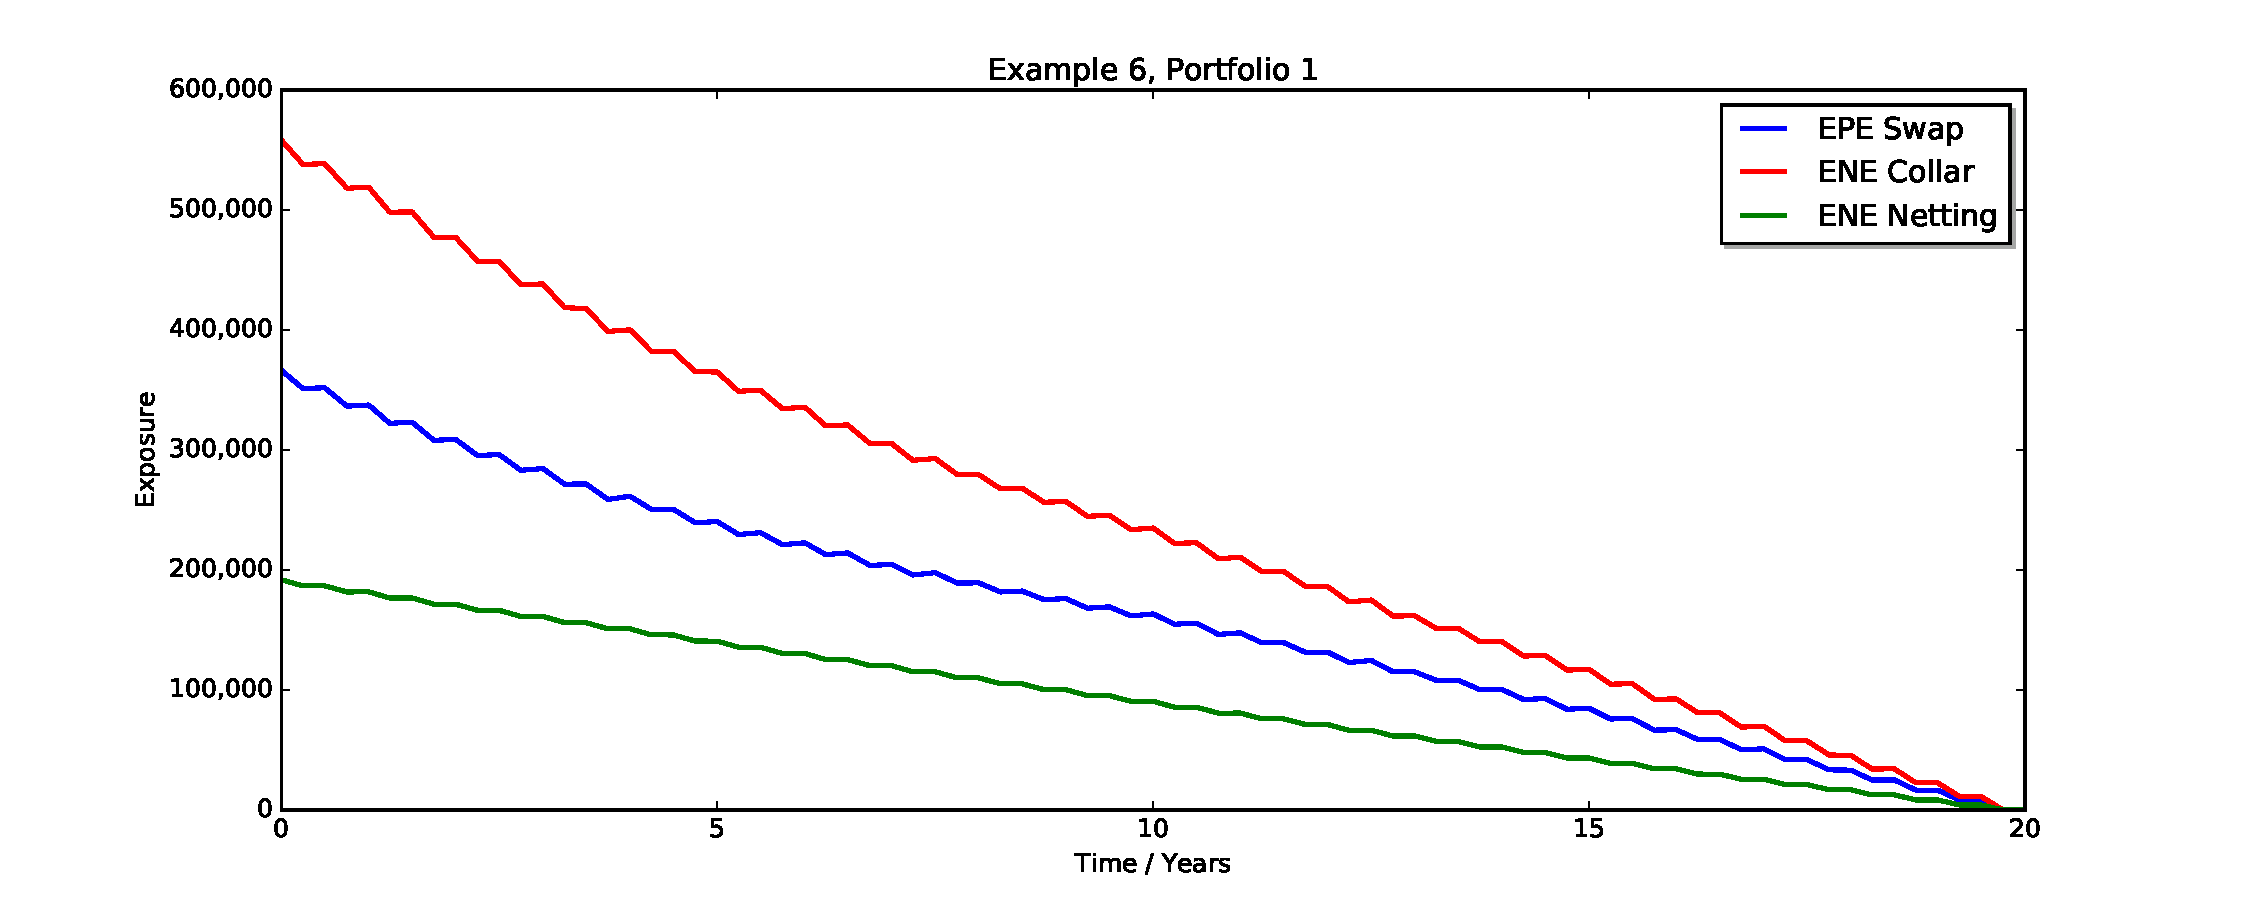
\includegraphics[scale=0.45]{mpl_capfloor_1.pdf}
\end{center}
\caption{Swap+Collar, portfolio 1. The Collar has identical cap and floor rates at 4\% so that it corresponds to a
  fixed leg which reduces the exposure of the Swap, which receives 3\% fixed. Simulation with 1000 paths and quarterly
  time steps.}
\label{fig_capfloor_1}
\end{figure}

The second example in this folder shown in figure \ref{fig_capfloor_2} ('portfolio 2') consists of a short Cap, long
Floor and a long Collar that exactly offsets the netted Cap and Floor.

\begin{figure}[h!]
\begin{center}
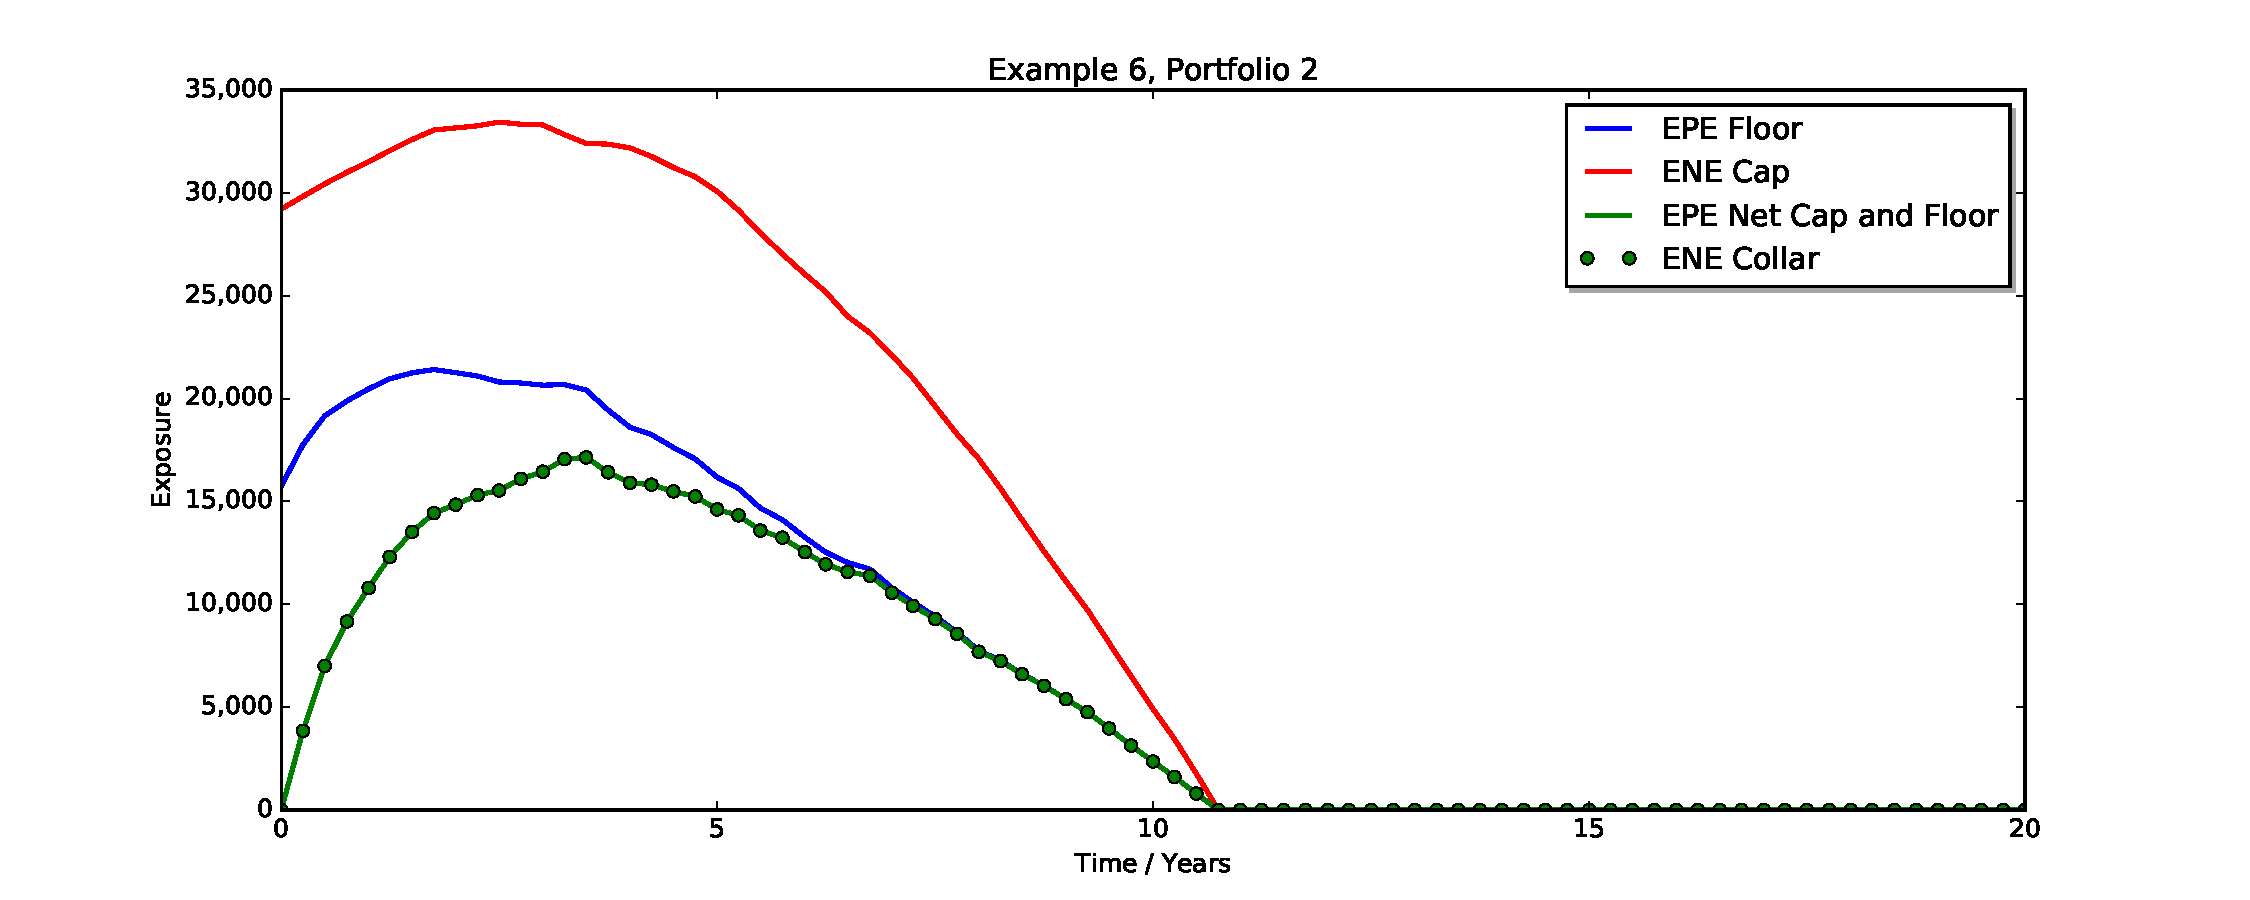
\includegraphics[scale=0.45]{mpl_capfloor_2.pdf}
\end{center}
\caption{Short Cap and long Floor vs long Collar, portfolio 2. Simulation with 1000 paths and quarterly time steps.}
\label{fig_capfloor_2}
\end{figure}

Further three test portfolios are provided as part of this example. Run the example and inspect the respective output
directories {\tt Examples/Example\_7/Output/portfolio\_\#}. Note that these directories have to be present/created
before running the batch with {\tt python run.py}.

%--------------------------------------------------------
\subsection{FX Forward Exposure}\label{sec:fxfwd}
%--------------------------------------------------------

The example in folder {\tt Examples/Example\_7} generates the exposure evolution for a EUR / USD FX Forward transaction
with value date in 10Y. This is a particularly simple show case because of the single cash flow in 10Y. On the other
hand it checks the cross currency model implementation by means of comparison to analytic limits - EPE and ENE at the
trade's value date must match corresponding Vanilla FX Option prices, as shown in figure \ref{fig_5}.
\begin{figure}[h]
\begin{center}
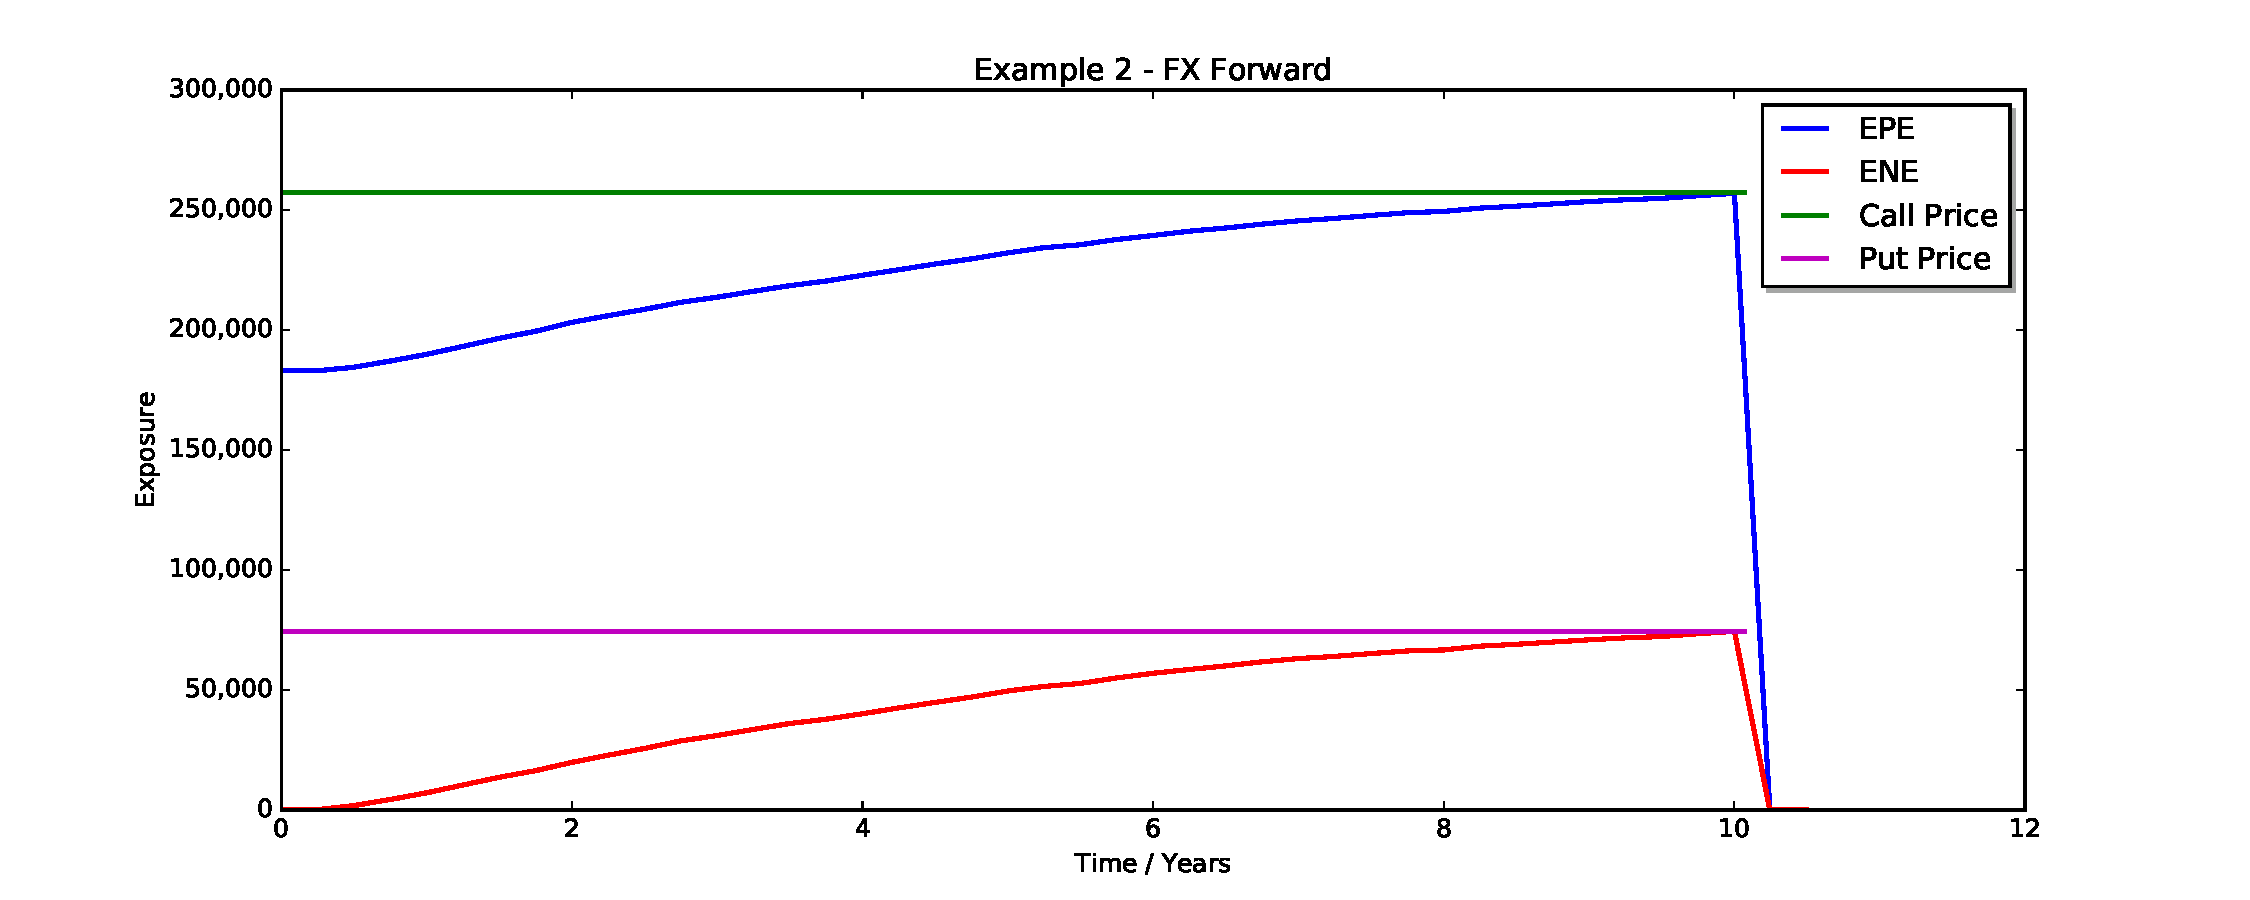
\includegraphics[scale=0.45]{mpl_fxforward.pdf}
\end{center}
\caption{EUR/USD FX Forward expected exposure in a realistic market environment as of 26/02/2016 from both parties'
  perspectives. Value date is obviously in 10Y. The flat lines are FX Option prices which coincide with EPE and ENE,
  respectively, on the value date. Simulation with 5000 paths and quarterly time steps.}
\label{fig_5}
\end{figure}

%--------------------------------------------------------
\subsection{FX Option Exposure}\label{sec:fxoption}
%--------------------------------------------------------

This example (in folder {\tt Examples/Example\_7}, as the FX Forward example) illustrates the exposure evolution for an
FX Option, see figure \ref{fig_7}.
\begin{figure}[h!]
\begin{center}
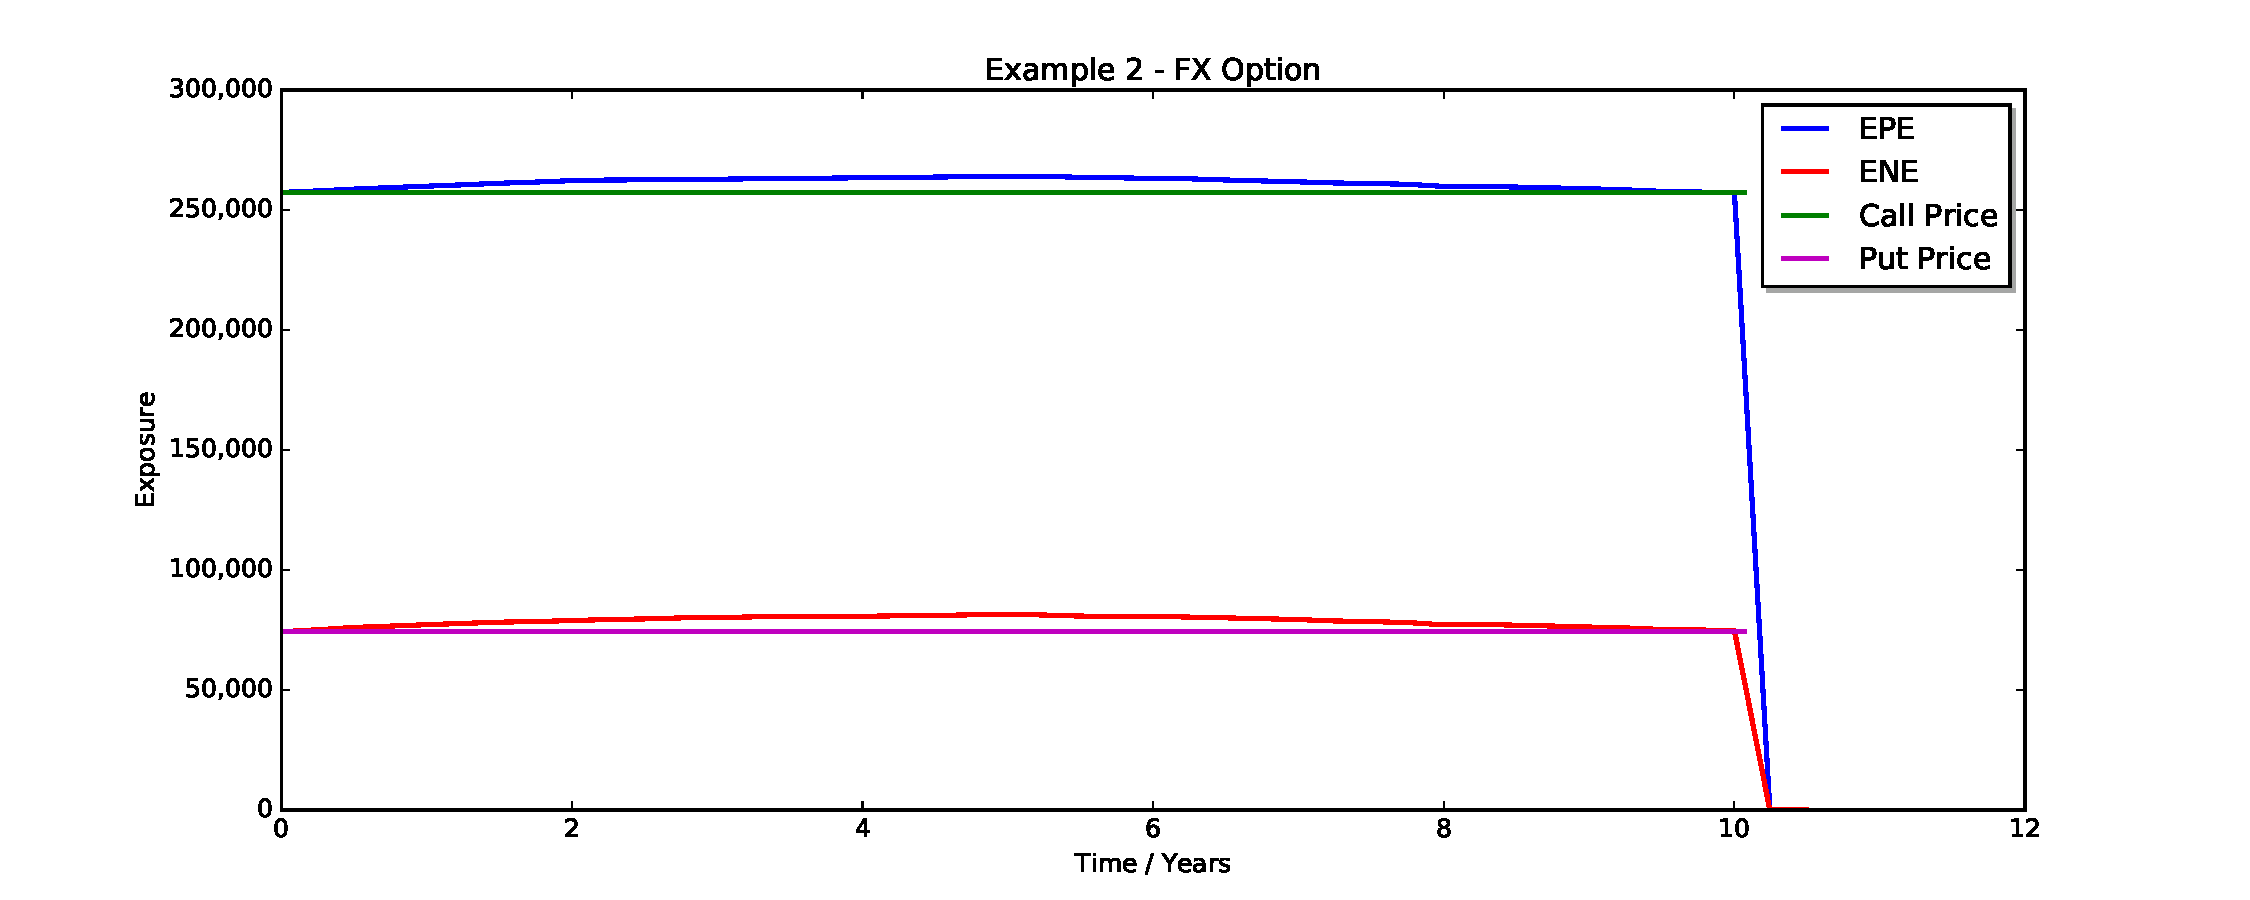
\includegraphics[scale=0.45]{mpl_fxoption.pdf}
\end{center}
\caption{EUR/USD FX Call and Put Option exposure evolution, same underlying and market data as in section
  \ref{sec:fxfwd}, compared to the call and put option price as of today (flat line). Simulation with 5000 paths and
  quarterly time steps.}
\label{fig_7}
\end{figure}
Recall that the FX Option value $NPV(t)$ as of time $0 \leq t \leq T$ satisfies
\begin{align*}
\frac{NPV(t)}{N(t)} &= \mbox{Nominal}\times\E_t\left[\frac{(X(T) - K)^+}{N(T)}\right]\\
NPV(0) &= \E\left[\frac{NPV(t)}{N(t)}\right] = \E\left[\frac{NPV^+(t)}{N(t)} \right]= \EPE(t) 
\end{align*}
One would therefore expect a flat exposure evolution up to option expiry. The deviation from this in ORE's simulation is
due to the pricing approach chosen here under scenarios. A Black FX option pricer is used with deterministic Black
volatility derived from today's volatility structure (pushed or rolled forward, see section \ref{sec:sim_market}). The
deviation can be removed by extending the volatility modelling, e.g. implying model consistent Black volatilities in
each simulation step on each path.  
%\todo[inline]{Add exposure evolution graph with 'simulated' FX vol}

%--------------------------------------------------------
\subsection{Cross Currency Swap Exposure and FX Reset}
%--------------------------------------------------------

The case in {\tt Examples/Example\_8} is a vanilla cross currency Swap. It shows the typical blend of an Interest Rate
Swap's saw tooth exposure evolution with an FX Forward's exposure which increases monotonically to final maturity, see
figure \ref{fig_6}.
\begin{figure}[h!]
\begin{center}
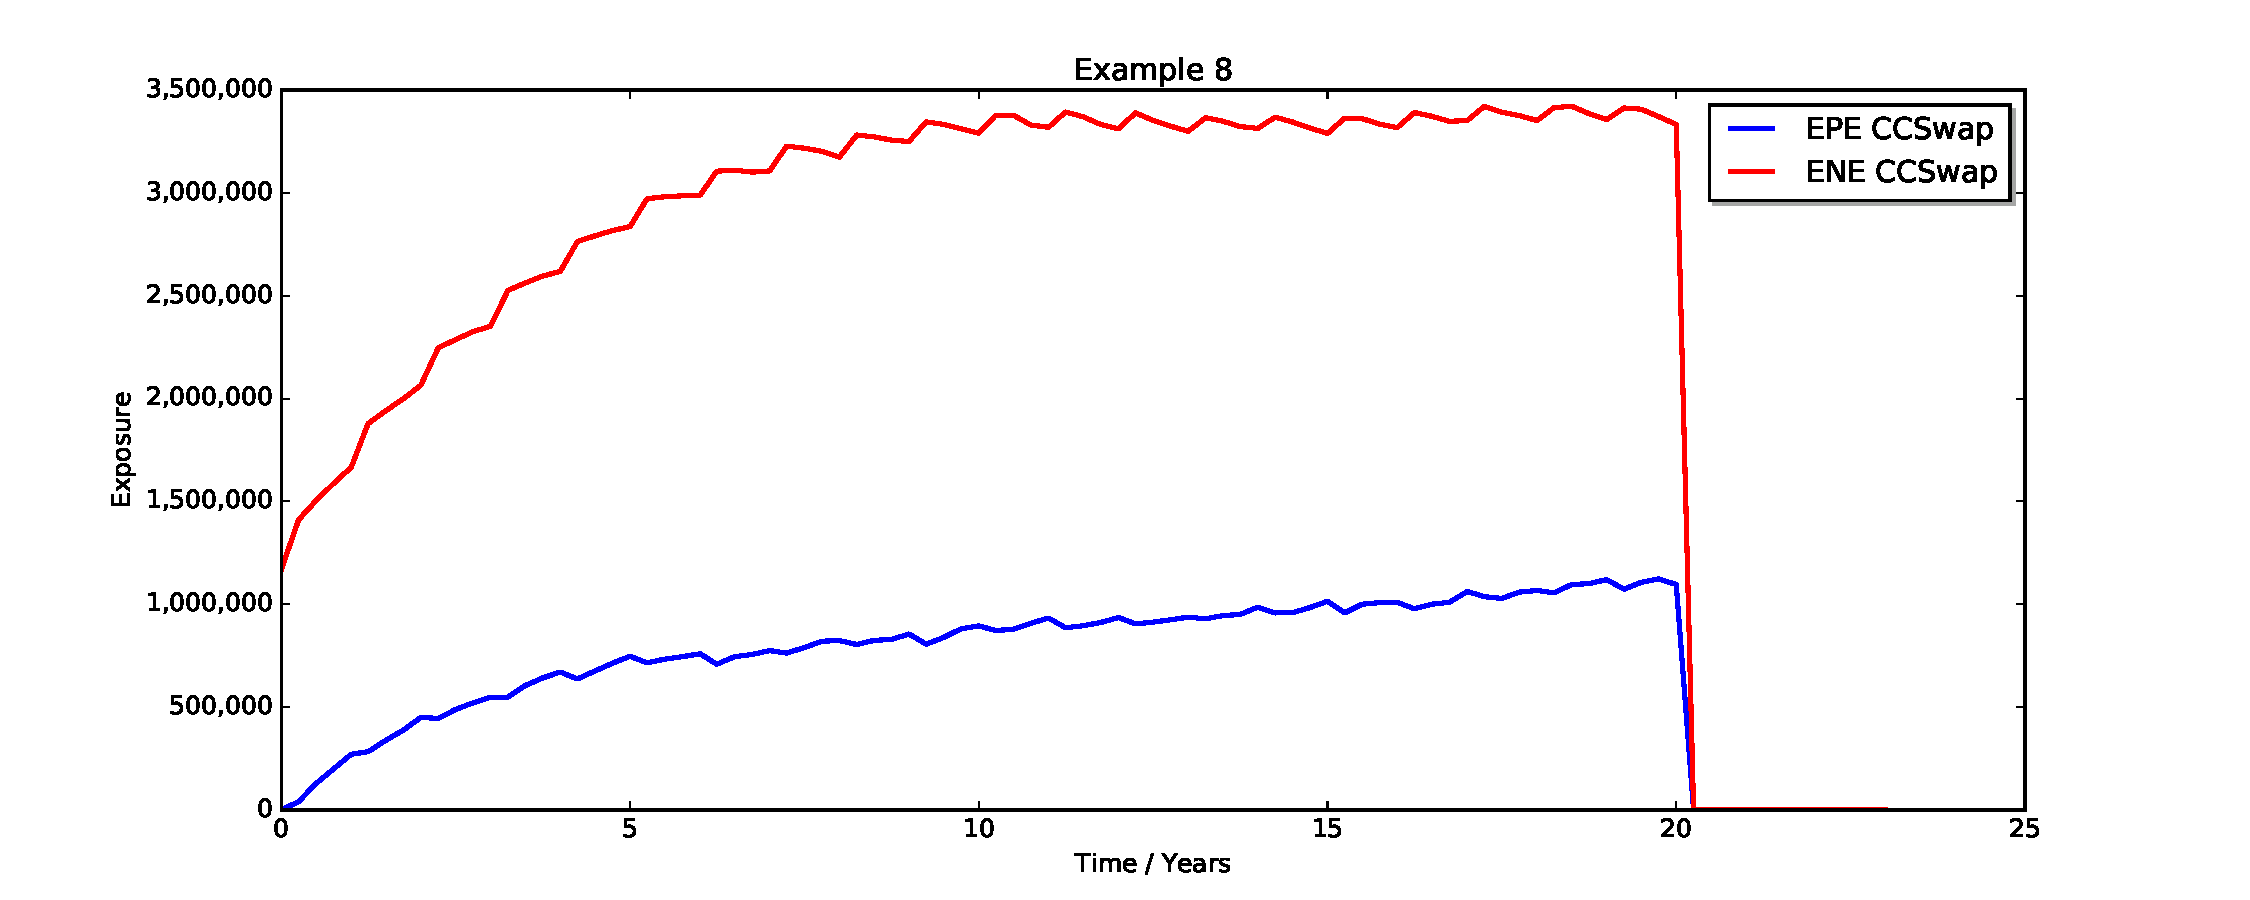
\includegraphics[scale=0.45]{mpl_ccswap.pdf}
\end{center}
\caption{Cross Currency Swap exposure evolution without mark-to-market notional reset. Simulation with 1000 paths and
  quarterly time steps.}
\label{fig_6}
\end{figure}

The effect of the FX resetting feature, common in Cross Currency Swaps nowadays, is shown in {\tt Examples/Example\_9}.
The example shows the exposure evolution of a EUR/USD cross currency basis Swap with FX reset at each interest period
start, see figure \ref{fig_6b}. As expected, the notional reset causes an exposure collapse at each period start when
the EUR leg's notional is reset to match the USD notional.
\begin{figure}[h!]
\begin{center}
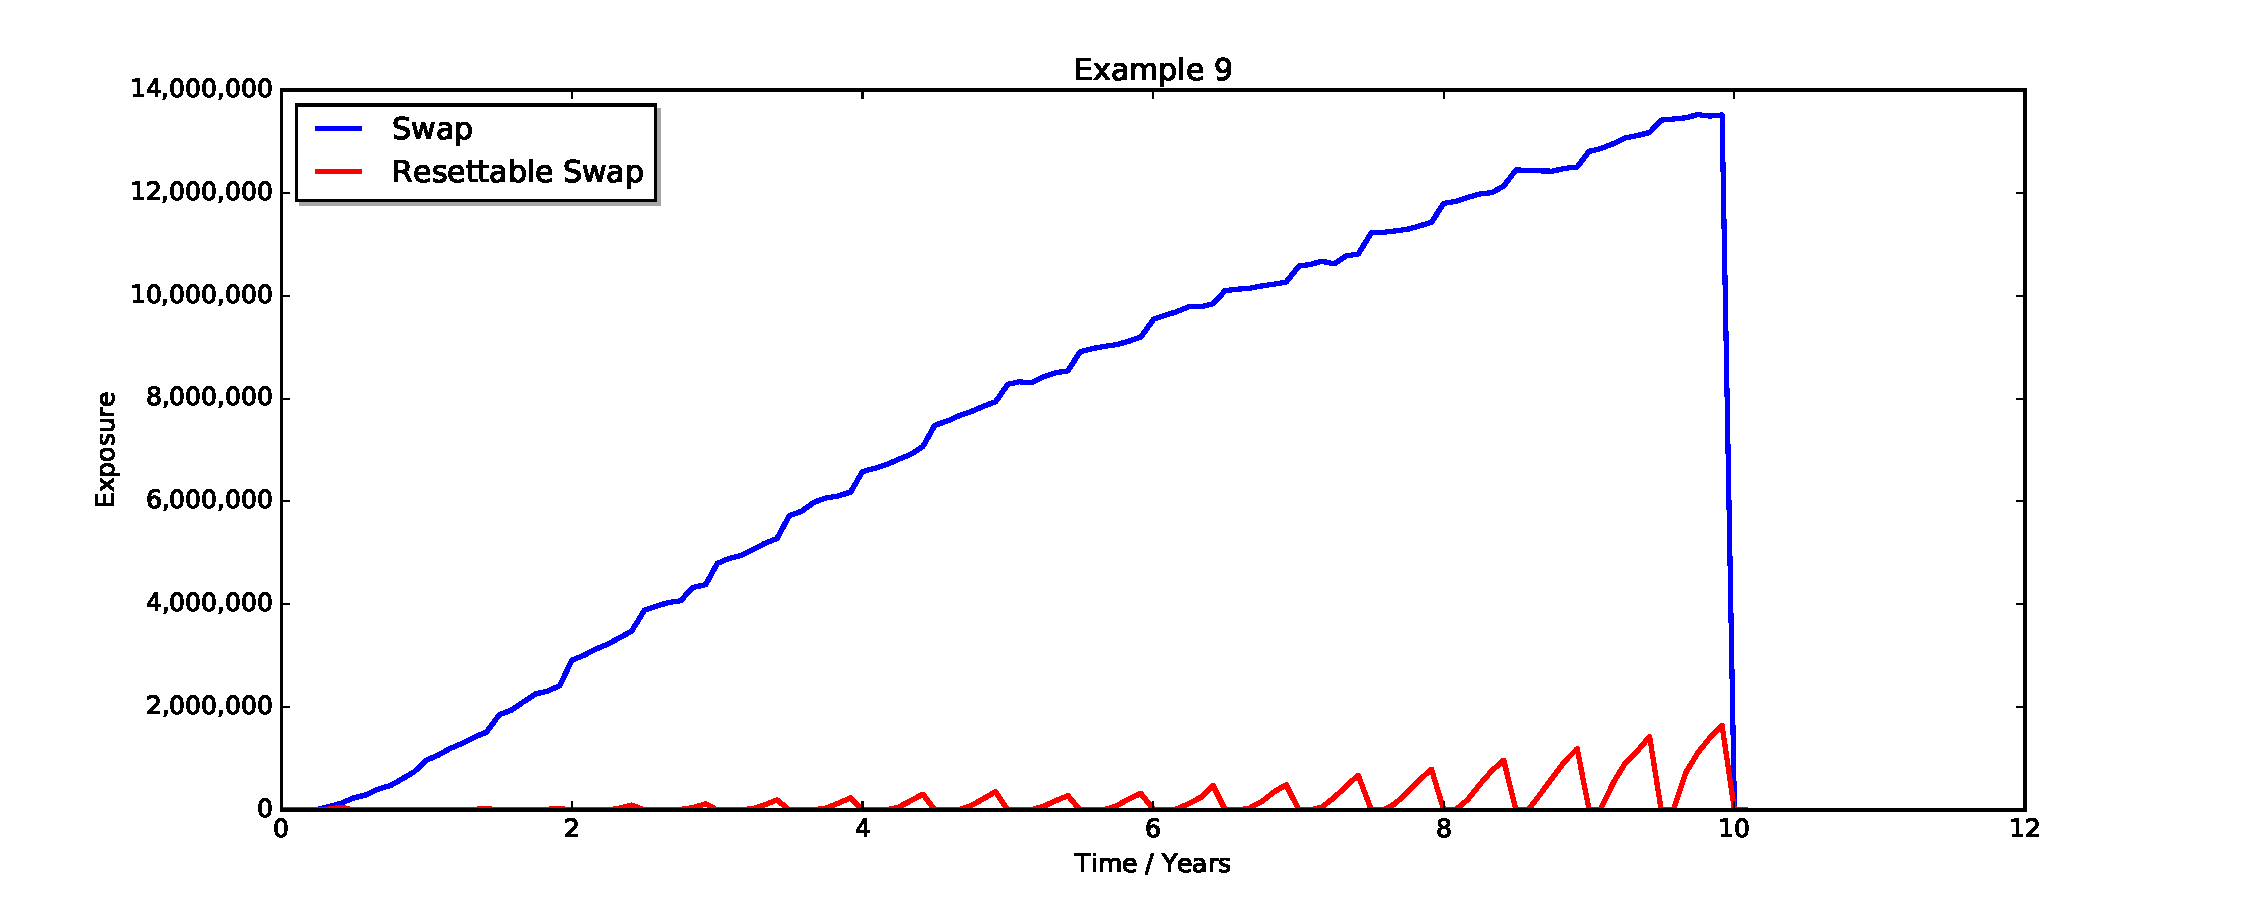
\includegraphics[scale=0.45]{mpl_xccy_reset.pdf}
\end{center}
\caption{Cross Currency Basis Swap exposure evolution with and without mark-to-market notional reset. Simulation with
  1000 paths and quarterly time steps.}
\label{fig_6b}
\end{figure}
  
%--------------------------------------------------------
\subsection{Netting and Collateral}
%--------------------------------------------------------

In this example (see folder {\tt Examples/Example\_10}) we showcase a small netting set consisting of three Swaps in
different currencies, with different collateral choices
\begin{itemize}
\item no collateral - figure \ref{fig_8},
\item collateral with threshold (THR) 1m EUR, minimum transfer amount (MTA) 100k EUR, margin period of risk (MPOR) 2
  weeks - figure \ref{fig_9}
\item collateral with zero THR and MTA, and MPOR 2w - figure \ref{fig_10}
\end{itemize}
The exposure graphs with collateral and positive margin period of risk show typical spikes. What is causing these? As
sketched in appendix \ref{sec:app_collateral}, ORE uses a {\em classical collateral model} that applies collateral
amounts to offset exposure with a time delay that corresponds to the margin period of risk. The spikes are then caused
by instrument cash flows falling between exposure measurement dates $d_1$ and $d_2$ (an MPOR apart), so that a
collateral delivery amount determined at $d_1$ but settled at $d_2$ differs significantly from the closeout amount at
$d_2$ causing a significant residual exposure for a short period of time. See for example \cite{Andersen2016} for a
recent detailed discussion of collateral modelling. The approach currently implemented in ORE corresponds to {\em
  Classical+} in \cite{Andersen2016}, the more conservative approach of the classical methods. The less conservative
alternative, {\em Classical-}, would assume that both parties stop paying trade flows at the beginning of the MPOR, so
that the P\&L over the MPOR does not contain the cash flow effect, and exposure spikes are avoided. Note that the size
and position of the largest spike in figure \ref{fig_9} is consistent with a cash flow of the 40 million GBP Swap in the
example's portfolio that rolls over the 3rd of March and has a cash flow on 3 March 2020, a bit more than four years
from the evaluation date.
  
\begin{figure}[h!]
\begin{center}
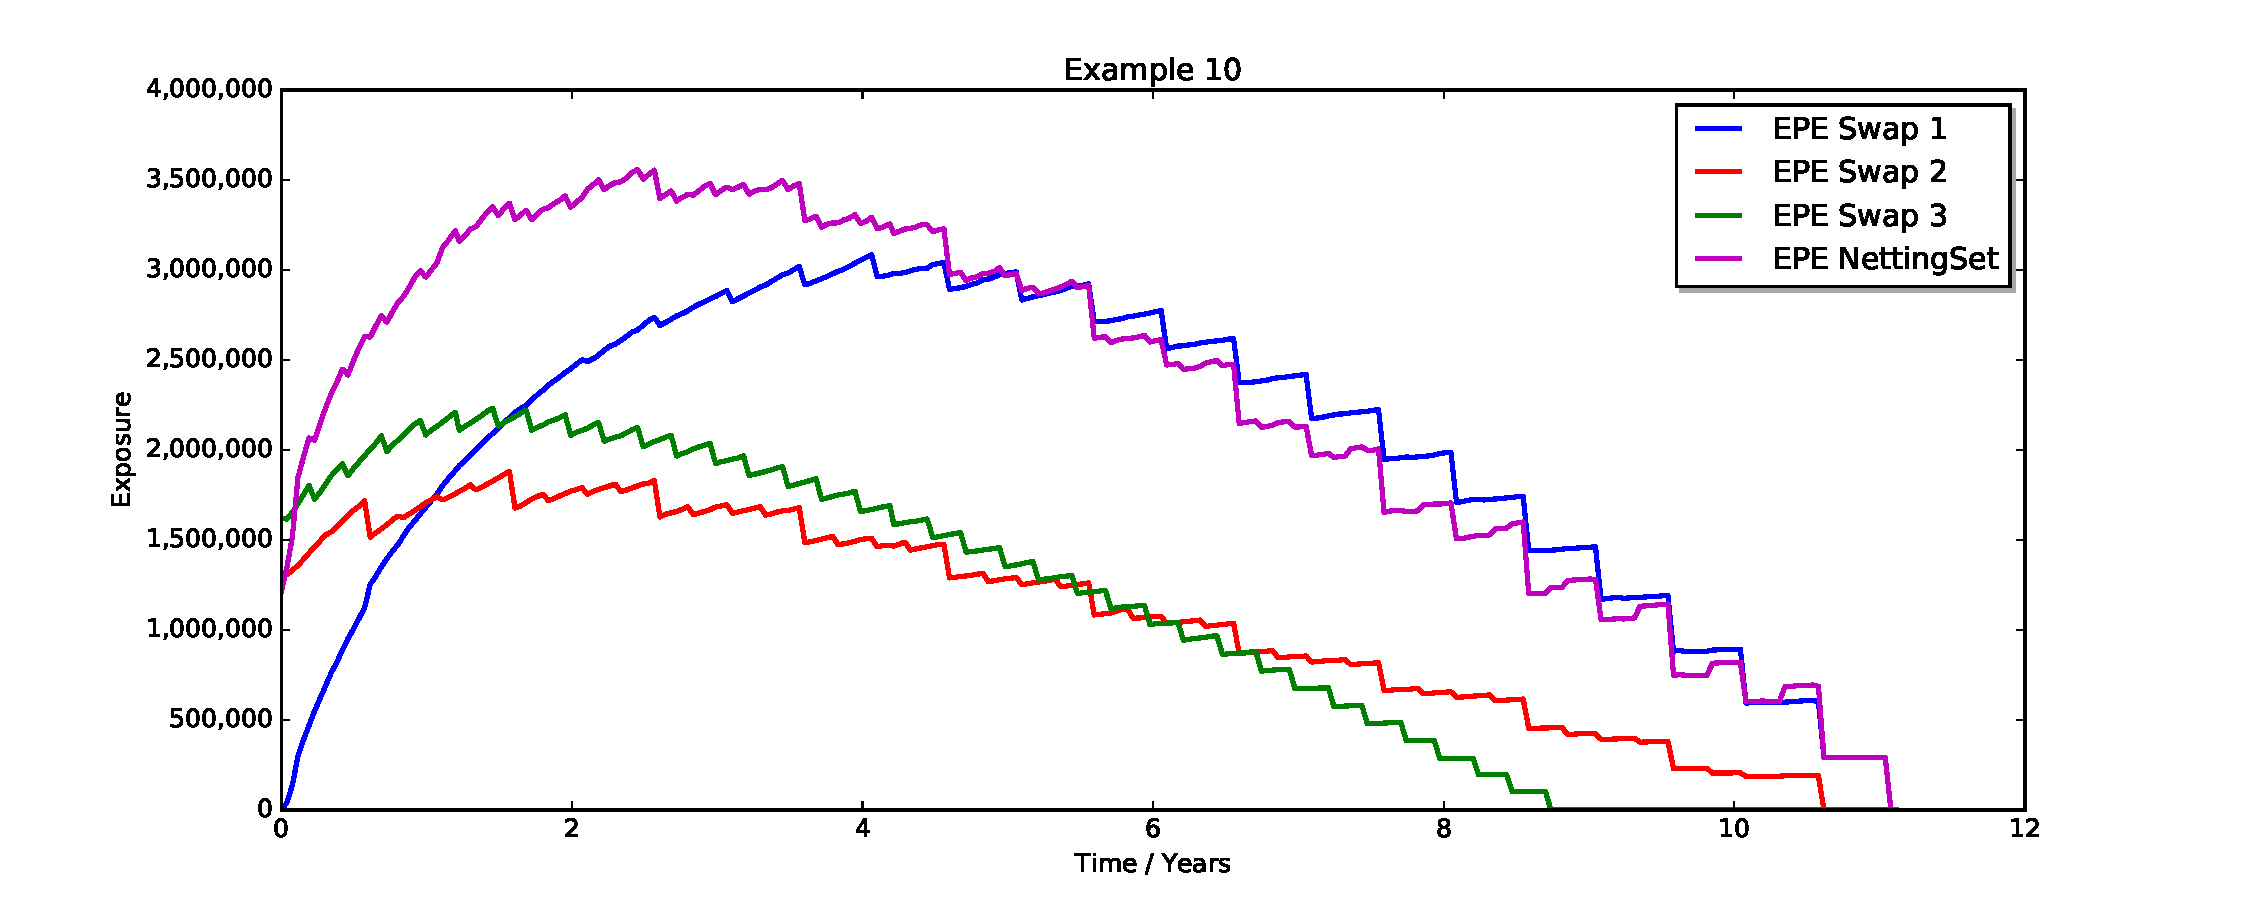
\includegraphics[scale=0.45]{mpl_nocollateral_epe.pdf}
\end{center}
\caption{Three Swaps netting set, no collateral. Simulation with 5000 paths and bi-weekly time steps.}
\label{fig_8}
\end{figure}

\begin{figure}[htb]
\begin{center}
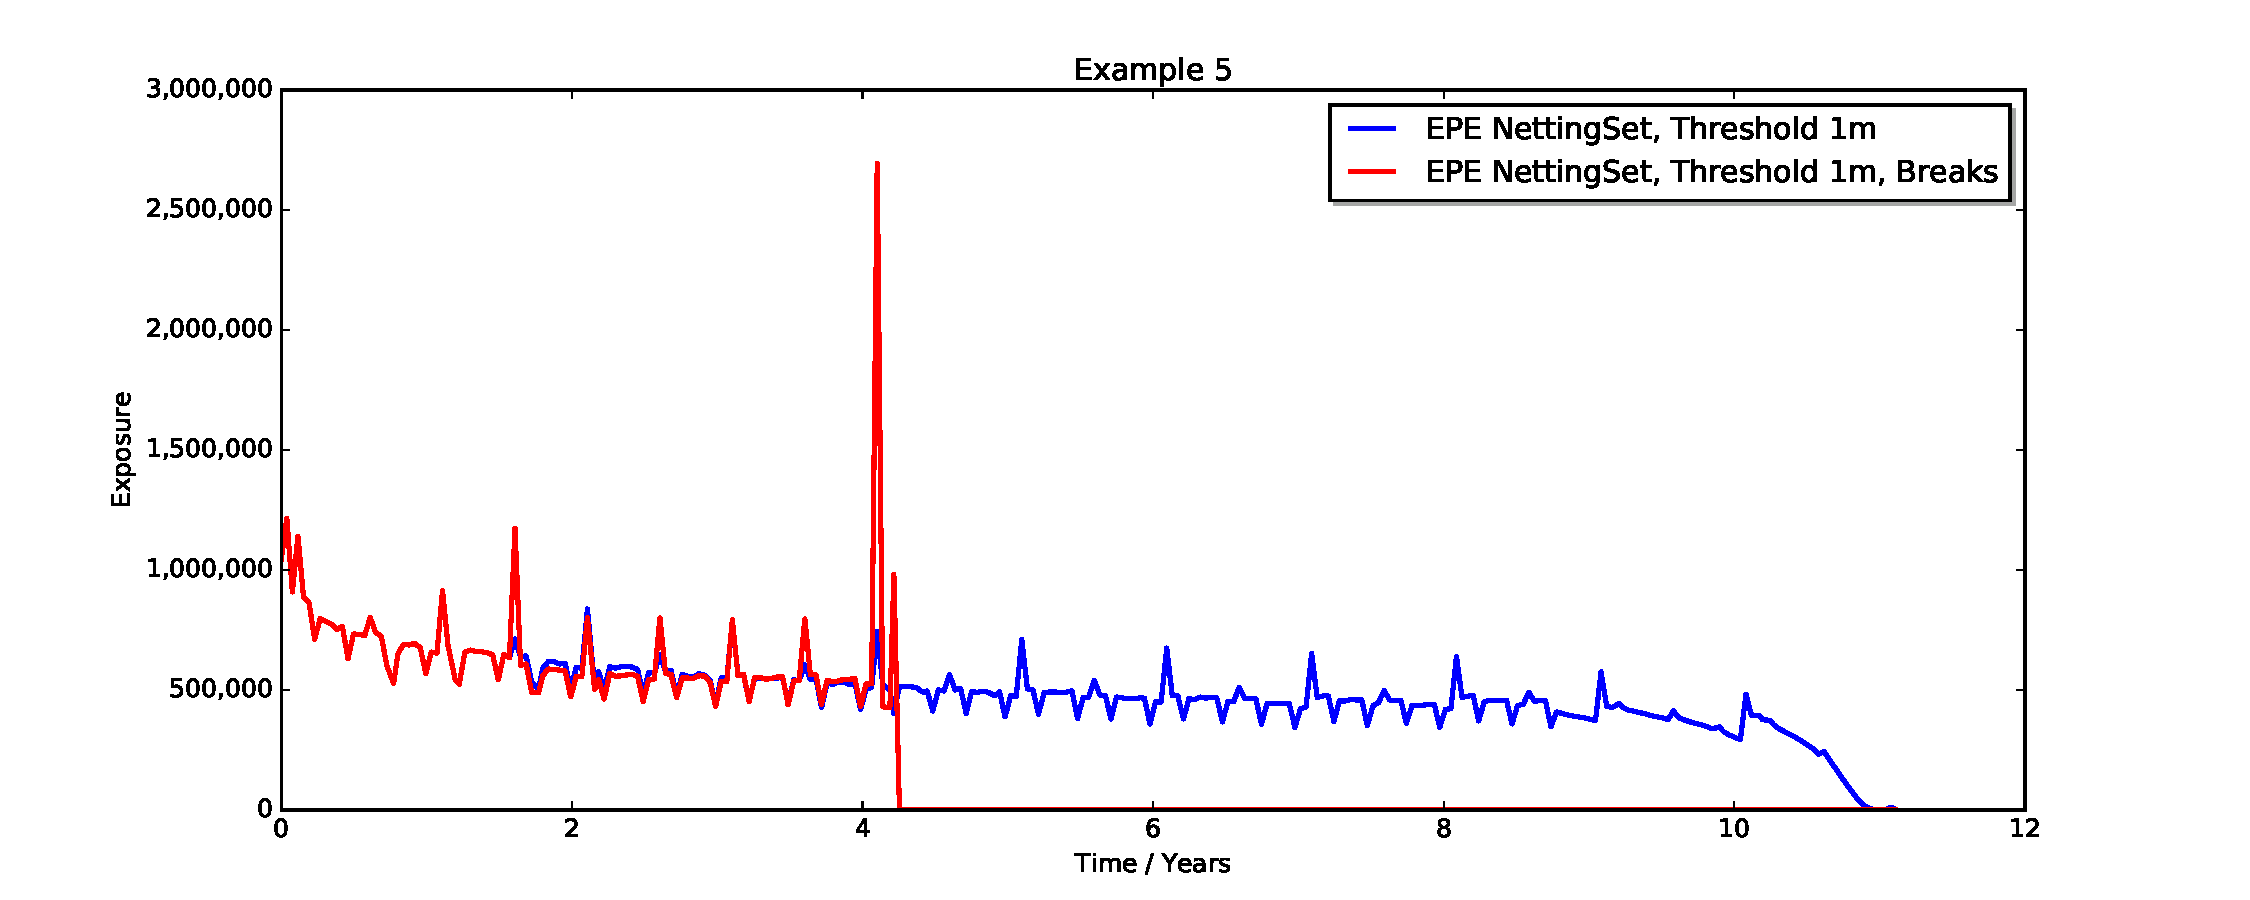
\includegraphics[scale=0.45]{mpl_threshold_break_epe.pdf}
\end{center}
\caption{Three Swaps netting set, THR=1m EUR, MTA=100k EUR, MPOR=2w. The red evolution assumes that the each trade is
  terminated at the next break date. The blue evolution ignores break dates. Simulation with 5000 paths and bi-weekly
  time steps.}
\label{fig_9}
\end{figure}

%\begin{figure}[h]
%\begin{center}
%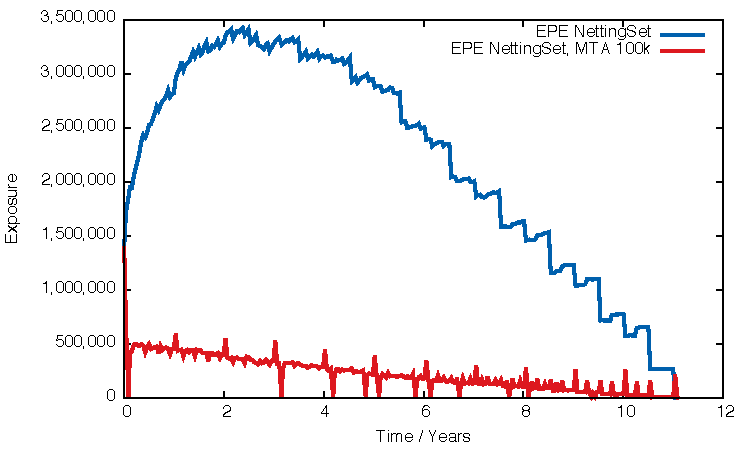
\includegraphics[scale=1.0]{example_mta_epe.pdf}
%\end{center}
%\caption{Three swaps, threshold = 0, mta > 0.}
%\label{fig_7}
%\end{figure}

\begin{figure}[h!]
\begin{center}
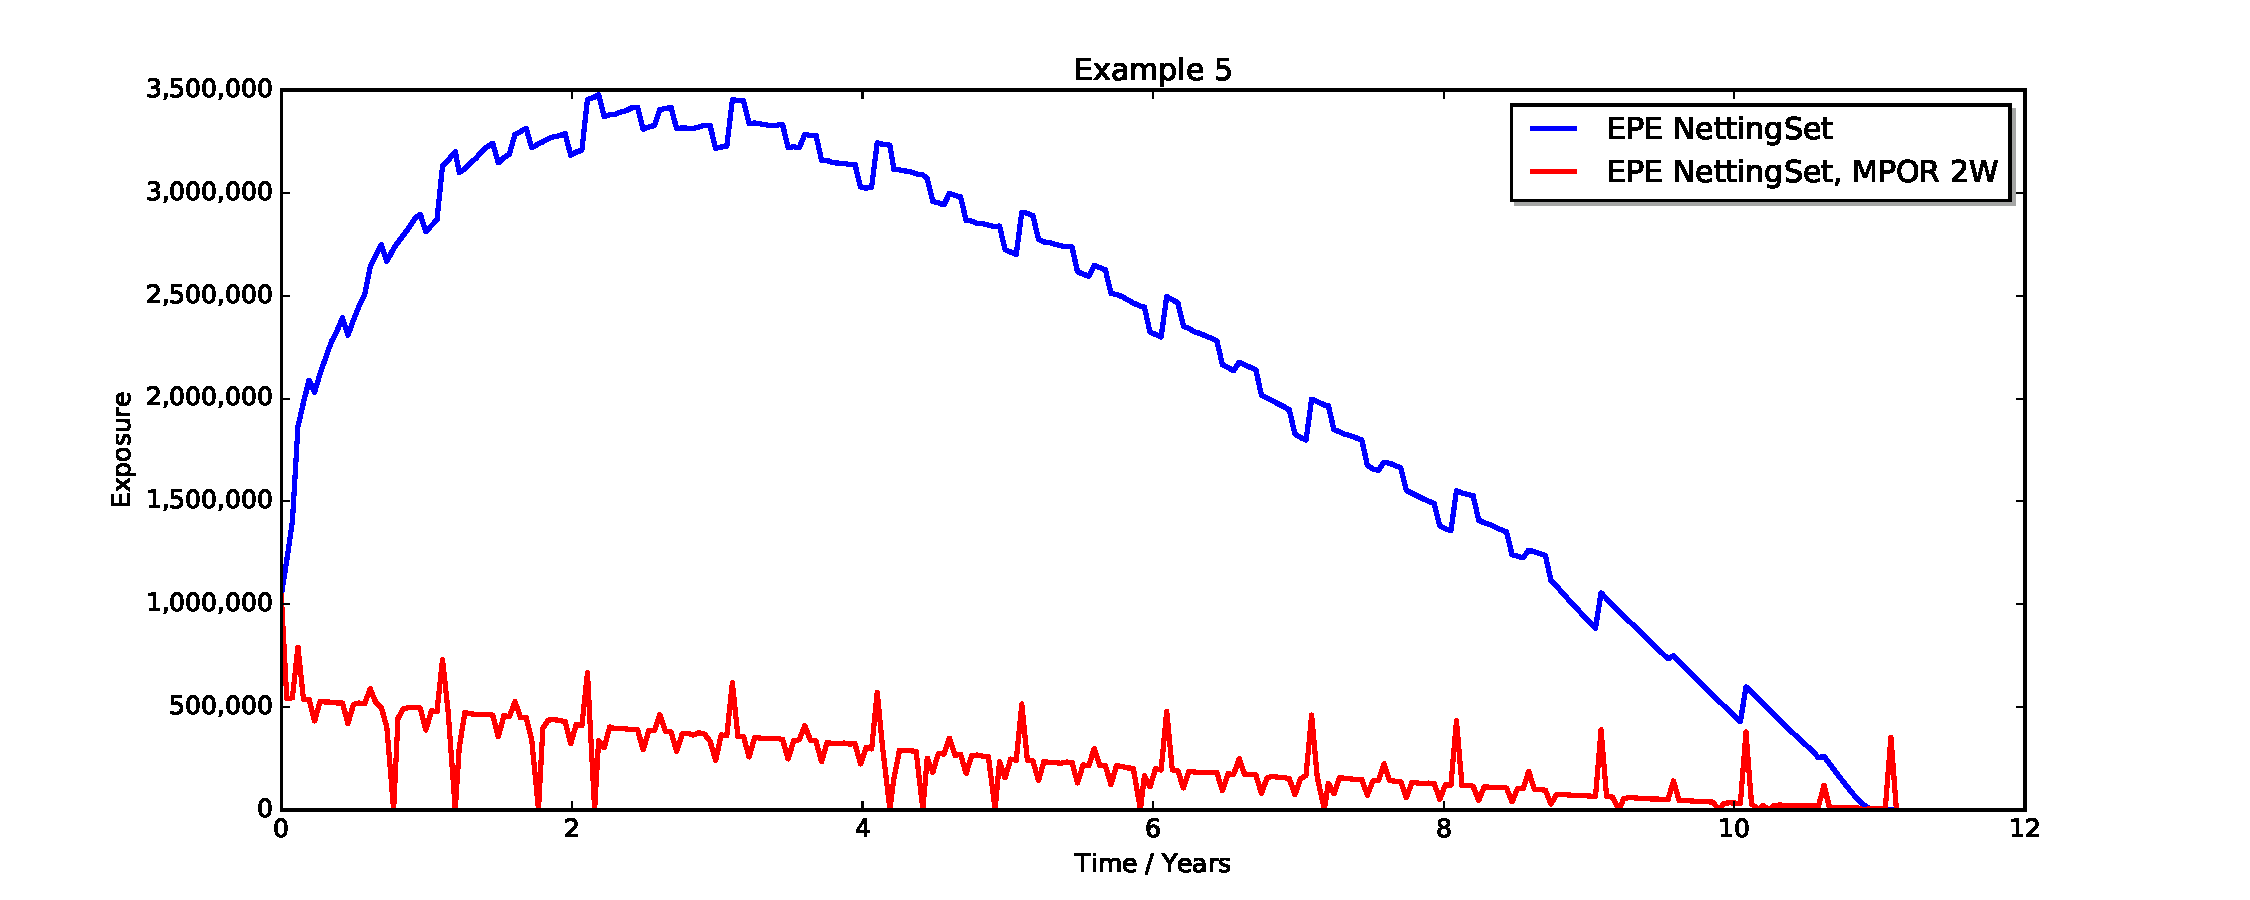
\includegraphics[scale=0.45]{mpl_mpor_epe.pdf}
\end{center}
\caption{Three Swaps, THR=MTA=0, MPOR=2w. Simulation with 5000 paths and bi-weekly time steps.}
\label{fig_10}
\end{figure}

%--------------------------------------------------------
\subsection{CVA, DVA, FVA, COLVA, MVA, Collateral Floor}
%--------------------------------------------------------

We use one of the cases in {\tt Examples/Example\_10} to demonstrate the
XVA outputs, see folder {\tt Examples/Example\_10/Output/collateral\_threshold\_dim}.

\medskip The summary of all value adjustments (CVA, DVA, FVA, COLVA, MVA, as well as the Collateral Floor) is provided
in file {\tt xva.csv}.  The file includes the allocated CVA and DVA numbers to individual trades as introduced in the
next section. The following table illustrates the file's layout, omitting the three columns containing allocated data.

\begin{center}
\resizebox{\columnwidth}{!}{%
\begin{tabular}{|l|l|r|r|r|r|r|r|r|r|r|}
\hline
TradeId & NettingSetId & CVA & DVA & FBA & FCA & COLVA & MVA & CollateralFloor & BaselEPE & BaselEEPE \\
\hline
 & CPTY\_A &  6,521  &  151,193  & -946  &  72,103  &  2,769  & -14,203  &  189,936  &  113,260  &  1,211,770 \\
Swap\_1 & CPTY\_A &  127,688  &  211,936  & -19,624  &  100,584  &  n/a  &  n/a  &  n/a   &  2,022,590  &  2,727,010 \\
Swap\_3 & CPTY\_A &  71,315  &  91,222  & -11,270  &  43,370  &  n/a  &  n/a  &  n/a   &  1,403,320  &  2,183,860 \\
Swap\_2 & CPTY\_A &  68,763  &  100,347  & -10,755  &  47,311  &  n/a  &  n/a  &  n/a   &  1,126,520  &  1,839,590 \\
\hline
\end{tabular}
}
\end{center}

The line(s) with empty TradeId column contain values at netting set level, the others contain uncollateralised
single-trade VAs.  Note that COLVA, MVA and Collateral Floor are only available at netting set level at which collateral
is posted.

\medskip
Detailed output is written for COLVA and Collateral Floor to file {\tt colva\_nettingset\_*.csv} which shows the 
incremental contributions to these two VAs through time.


%--------------------------------------------------------
\subsection{Exposure Reports \& XVA Allocation to Trades}
%--------------------------------------------------------
Using the example in folder {\tt Examples/Example\_10} we illustrate here the layout of an exposure report produced by
ORE. The report shows the exposure evolution of Swap\_1 without collateral which - after running Example\_10 - is found
in folder \\
{\tt Examples/Example\_10/Output/collateral\_none/exposure\_trade\_Swap\_1.csv}:

\begin{center}
\resizebox{\columnwidth}{!}{%
\begin{tabular}{|l|l|r|r|r|r|r|r|r|r|}
\hline
TradeId & Date & Time & EPE & ENE & AllocEPE & AllocENE & PFE & BaselEE & BaselEEE \\
\hline
Swap\_1 & 05/02/16 & 0.0000 & 0  & 1,711,748  & 0  & 0  & 0  & 0  & 0 \\
Swap\_1 & 19/02/16 & 0.0383 & 38,203   & 1,749,913  & -1,200,677 & 511,033 & 239,504 & 38,202 & 38,202 \\
Swap\_1 & 04/03/16 & 0.0765 & 132,862  & 1,843,837 & -927,499 & 783,476 & 1,021,715 & 132,845 & 132,845 \\
%Swap\_1 & 18/03/16 & 0.1148 & 299,155  & 1,742,450  & -650,225  & 793,067  & 1,914,150  & 299,091  & 299,091 \\
%Swap\_1 & 01/04/16 & 0.1530 & 390,178  & 1,834,810  & -552,029  & 892,604  & 2,373,560  & 390,058  & 390,058 \\
%Swap\_1 & 15/04/16 & 0.1913 & 471,849  & 1,918,600  & -465,580  & 981,171  & 2,765,710  & 471,659  & 471,659 \\
%Swap\_1 & 29/04/16 & 0.2295 & 550,301  & 2,000,640  & -330,578  & 1,119,760  & 3,106,810  & 550,016  & 550,016 \\
%Swap\_1 & 13/05/16 & 0.2678 & 620,279  & 2,074,880  & -266,042  & 1,188,560  & 3,427,080  & 619,888  & 619,888 \\
%Swap\_1 & 27/05/16 & 0.3060 & 690,018  & 2,140,320  & -190,419  & 1,259,880  & 3,778,570  & 689,509  & 689,509 \\
%Swap\_1 & 10/06/16 & 0.3443 & 763,207  & 2,206,020  & -137,681  & 1,305,130  & 4,052,870  & 762,560  & 762,560 \\
Swap\_1 & ... & ...& ... & ... & ... & ... & ... & ... & ... \\
\hline
\end{tabular}
}
\end{center}

The exposure measures EPE, ENE and PFE, and the Basel exposure measures $EE_B$ and $EEE_B$, are defined in appendix
\ref{sec:app_exposure}. Allocated exposures are defined in appendix \ref{sec:app_allocation}. The PFE quantile and
allocation method are chosen as described in section \ref{sec:analytics}. \\

In addition to single trade exposure files, ORE produces an exposure file per netting set. The example from the same
folder as above is:

\begin{center}
\resizebox{\columnwidth}{!}{%
\begin{tabular}{|l|l|r|r|r|r|r|r|r|}
\hline
NettingSet & Date & Time & EPE & ENE & PFE & ExpectedCollateral & BaselEE & BaselEEE \\
\hline
CPTY\_A & 05/02/16 & 0.0000 & 1,203,836 & 0 & 1,203,836 & 0 & 1,203,836 & 1,203,836 \\%1,211,770 & 0 & 1,211,770 & 0 & 1,211,770 & 1,211,770\\
CPTY\_A & 19/02/16 & 0.0383 & 1,337,713 & 137,326 & 3,403,460 & 0 & 1,337,651 & 1,337,651 \\ %0.0383 & 1,344,220 & 137,776 & 3,414,000 & 0 & 1,344,160 & 1,344,160\\
%CPTY\_A & 04/03/16 & 0.0765 & 1,518,610 & 308,381 & 4,354,060 & 0 & 1,518,410 & 1,518,410\\
%CPTY\_A & 18/03/16 & 0.1148 & 1,846,900 & 382,068 & 5,200,730 & 0 & 1,846,500 & 1,846,500\\
%CPTY\_A & 01/04/16 & 0.1530 & 1,961,290 & 494,416 & 5,869,470 & 0 & 1,960,690 & 1,960,690\\
%CPTY\_A & 15/04/16 & 0.1913 & 2,067,240 & 598,283 & 6,384,140 & 0 & 2,066,400 & 2,066,400\\
%CPTY\_A & 29/04/16 & 0.2295 & 2,053,670 & 745,960 & 6,740,070 & 0 & 2,052,610 & 2,066,400\\
%CPTY\_A & 13/05/16 & 0.2678 & 2,149,190 & 845,507 & 6,930,230 & 0 & 2,147,840 & 2,147,840\\
%CPTY\_A & 27/05/16 & 0.3060 & 2,235,630 & 930,218 & 7,295,440 & 0 & 2,233,980 & 2,233,980\\
%CPTY\_A & 10/06/16 & 0.3443 & 2,314,470 & 1,014,690 & 7,753,190 & 0 & 2,312,510 & 2,312,510\\
CPTY\_A & ... & ...& ... & ... & ... & ... & ... & ...\\
%CPTY\_A & 07/07/17 & 1.4167 & 3,320,430 & 2,423,890 & 12,787,900 & 0 & 3,304,650 & 3,304,650\\
%CPTY\_A & 21/07/17 & 1.4551 & 3,351,780 & 2,452,640 & 12,964,200 & 0 & 3,335,420 & 3,335,420\\
%CPTY\_A & 04/08/17 & 1.4934 & 3,302,820 & 2,511,500 & 12,796,100 & 0 & 3,286,260 & 3,335,420\\
%CPTY\_A & 18/08/17 & 1.5318 & 3,339,840 & 2,545,850 & 13,120,000 & 0 & 3,322,640 & 3,335,420\\
%CPTY\_A & 01/09/17 & 1.5701 & 3,371,300 & 2,576,100 & 13,238,700 & 0 & 3,353,480 & 3,353,480\\
%CPTY\_A & 15/09/17 & 1.6085 & 3,279,670 & 2,555,370 & 13,041,300 & 0 & 3,261,880 & 3,353,480\\
%CPTY\_A & 29/09/17 & 1.6468 & 3,305,060 & 2,579,200 & 13,072,800 & 0 & 3,286,680 & 3,353,480\\
%CPTY\_A & 13/10/17 & 1.6852 & 3,332,830 & 2,604,200 & 13,225,600 & 0 & 3,313,850 & 3,353,480\\
%CPTY\_A & 27/10/17 & 1.7236 & 3,280,280 & 2,661,770 & 13,034,600 & 0 & 3,261,150 & 3,353,480\\
%CPTY\_A & 13/11/17 & 1.7701 & 3,316,800 & 2,701,060 & 13,331,600 & 0 & 3,296,880 & 3,353,480\\
%CPTY\_A & 24/11/17 & 1.8003 & 3,337,760 & 2,720,870 & 13,402,400 & 0 & 3,317,280 & 3,353,480\\
%CPTY\_A & ... & ...& ... & ... & ... & ... & ... & ...\\
\hline
\end{tabular}
}
\end{center}

Allocated exposures are missing here, as they make sense at the trade level only, and the expected collateral balance is
added for information (in this case zero as collateralisation is deactivated in this example).

\medskip The allocation of netting set exposure and XVA to the trade level is frequently required by finance
departments. This allocation is also featured in {\tt Examples/Example\_10}. We start again with the uncollateralised
case in figure \ref{fig_12}, followed by the case with threshold 1m EUR in figure \ref{fig_13}.
\begin{figure}[h!]
\begin{center}
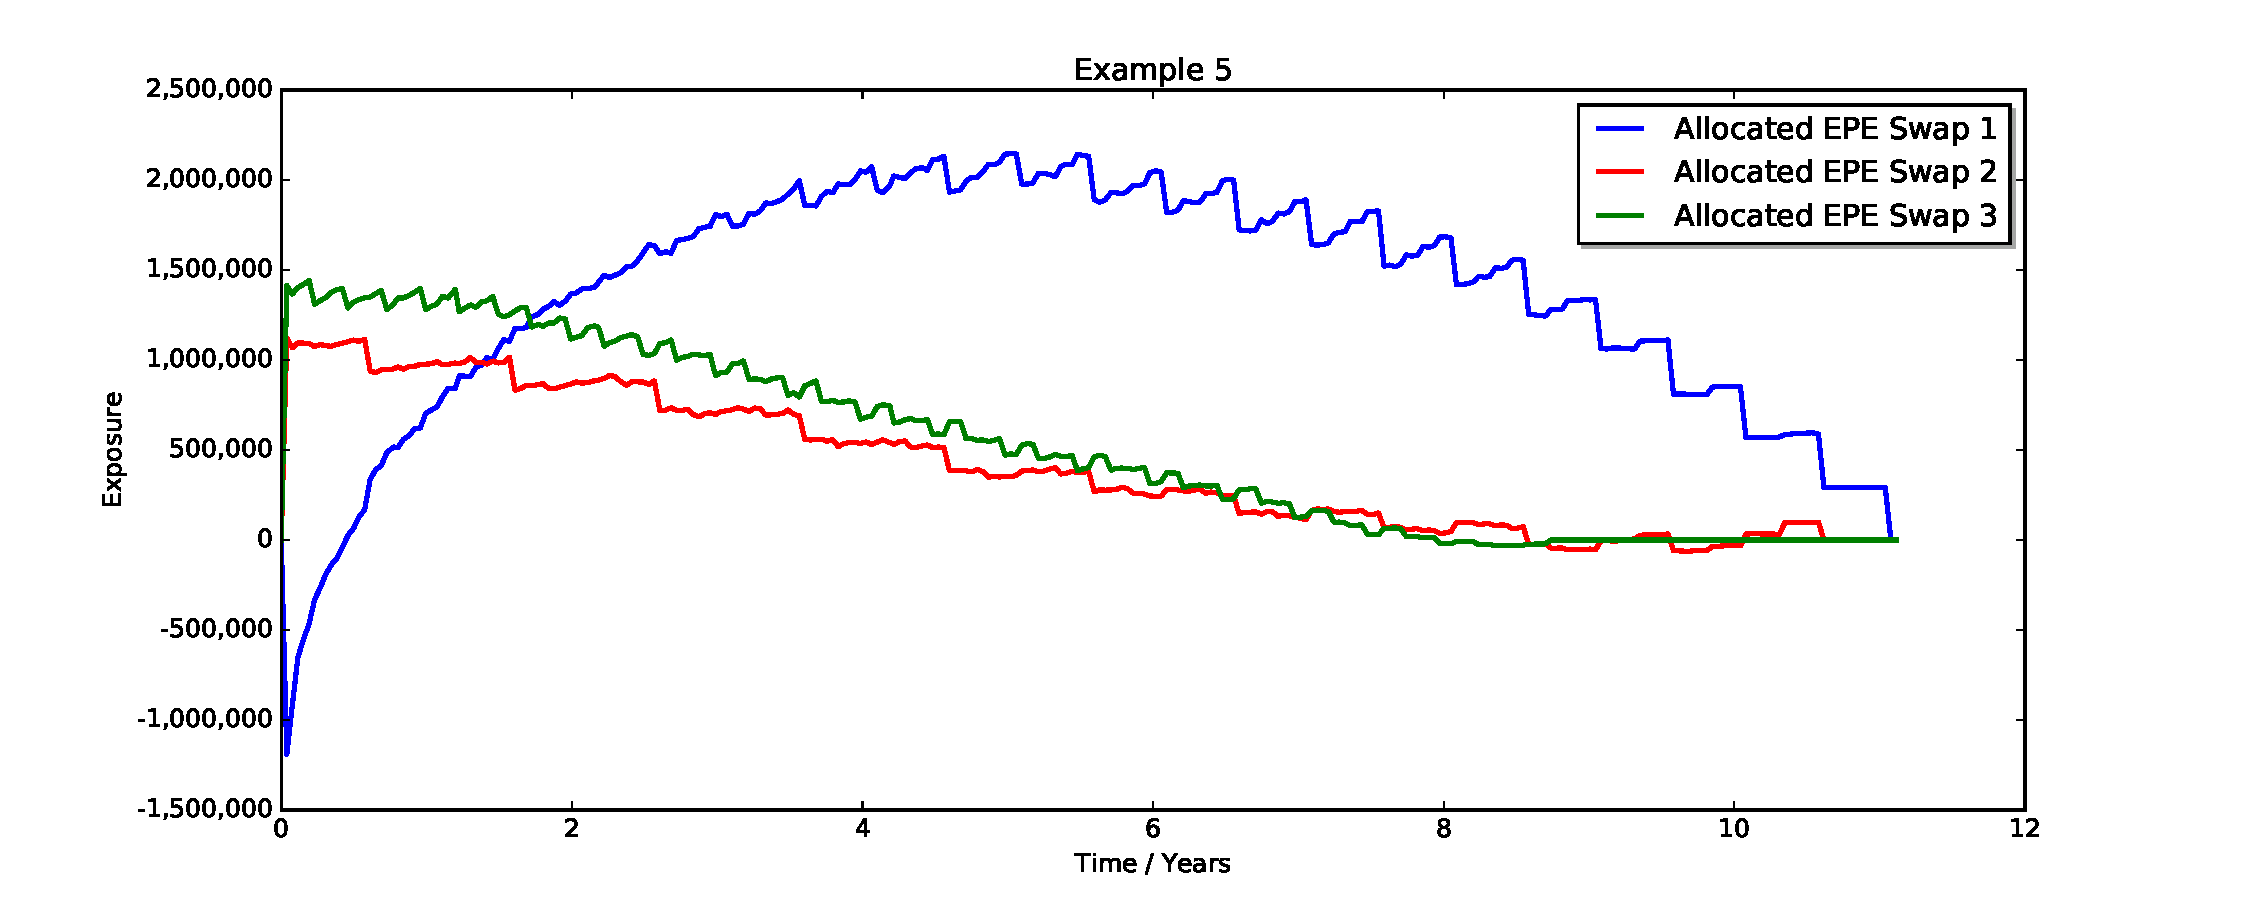
\includegraphics[scale=0.45]{mpl_nocollateral_allocated_epe.pdf}
\end{center}
\caption{Exposure allocation without collateral. Simulation with 5000 paths and bi-weekly time steps.}
\label{fig_12}
\end{figure}
In both cases we apply the {\em marginal} (Euler) allocation method as published by Pykhtin and Rosen in 2010, hence we
see the typical negative EPE for one of the trades at times when it reduces the netting set exposure. The case with
collateral moreover shows the typical spikes in the allocated exposures.
\begin{figure}[h!]
\begin{center}
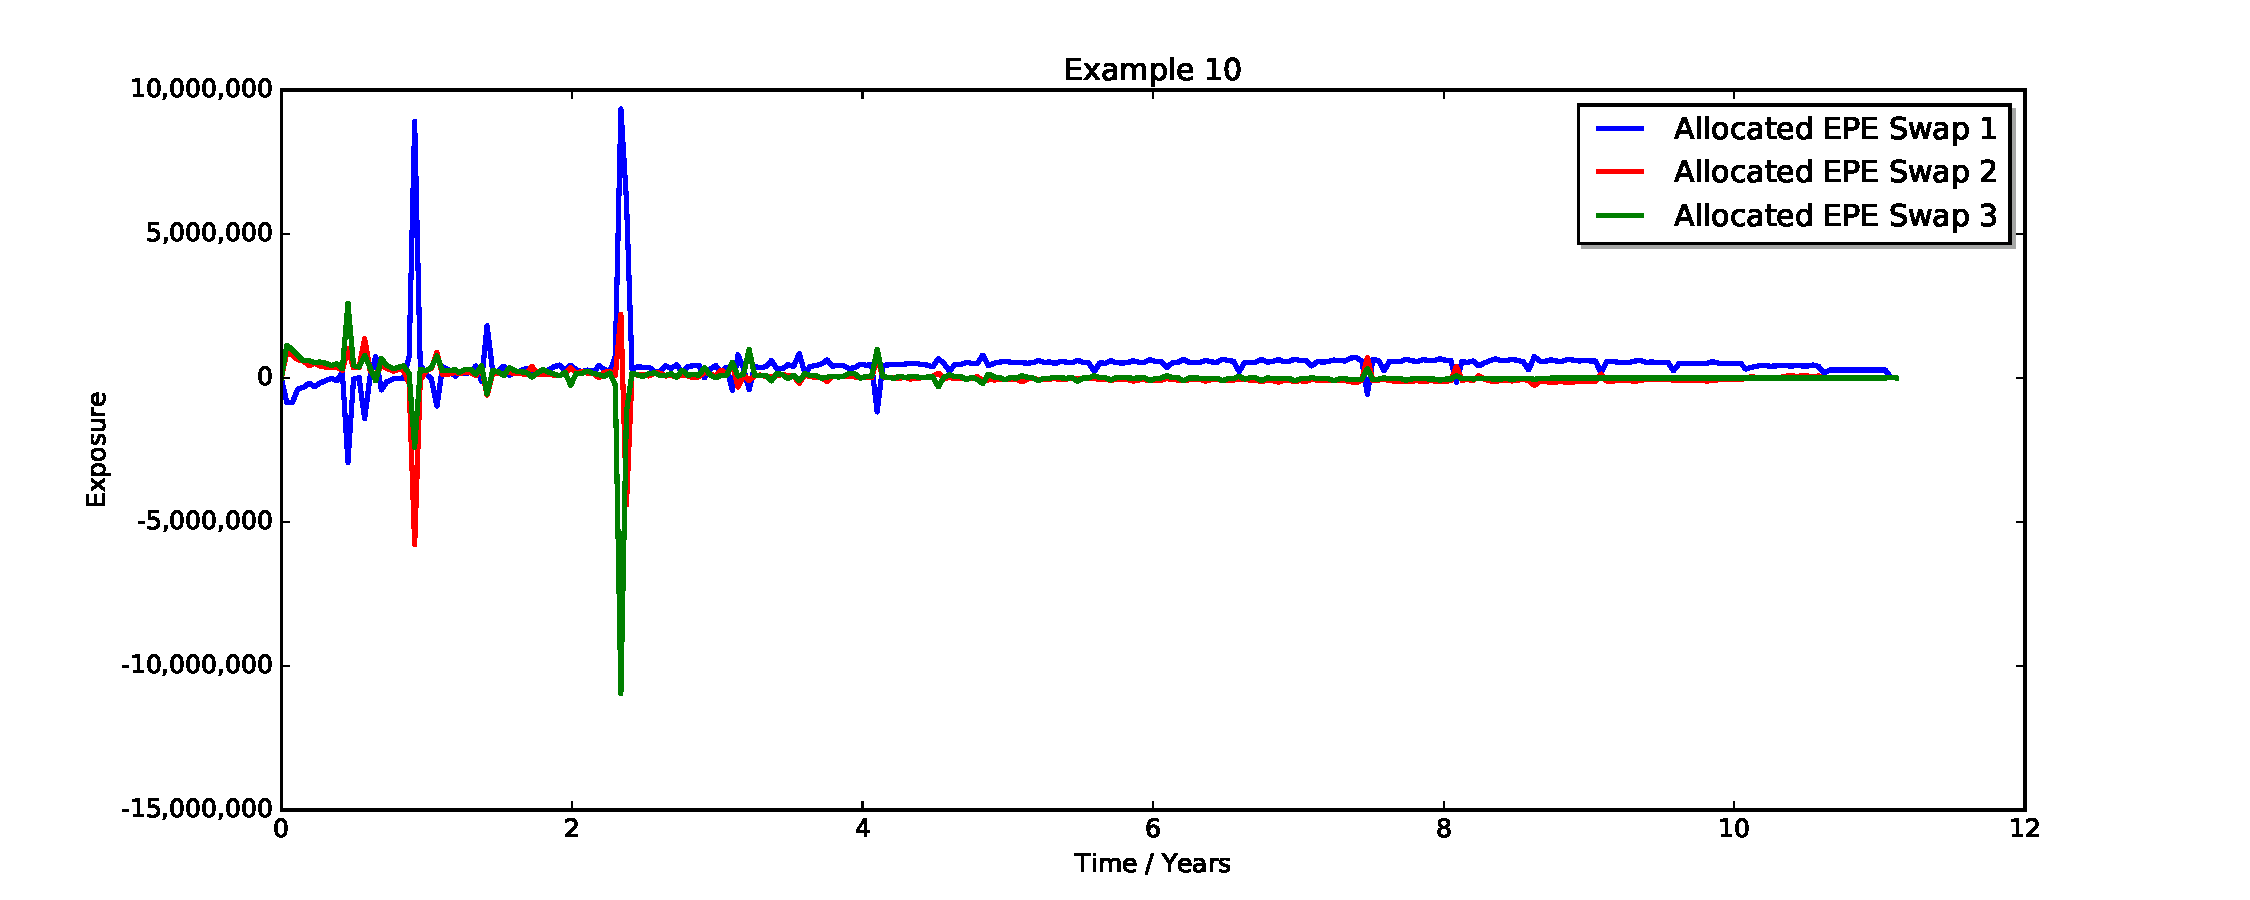
\includegraphics[scale=0.45]{mpl_threshold_allocated_epe.pdf}
\end{center}
\caption{Exposure allocation with collateral and threshold 1m EUR. Simulation with 5000 paths and bi-weekly time steps.}
\label{fig_13}
\end{figure}
The analytics results also feature allocated XVAs in file {\tt xva.csv} which are derived from the allocated exposure
profiles. Note that ORE also offers alternative allocation methods to the marginal method by Pykhtin/Rosen, which can be
explored with {\tt Examples/Example\_10}.

%--------------------------------------------------------
\subsection{Basel Exposure Measures}\label{sec:basel}
%--------------------------------------------------------

Example {\tt Example\_11} demonstrates the relation between the evolution of the expected exposure (EPE in our notation)
to the `Basel' exposure measures EE\_B, EEE\_B, EPE\_B and EEPE\_B as defined in appendix \ref{sec:app_exposure}. In
particular the latter is used in internal model methods for counterparty credit risk as a measure for the exposure at
default. It is a `derivative' of the expected exposure evolution and defined as a time average over the running maximum
of EE\_B up to the horizon of one year.
\begin{figure}[h!]
\begin{center}
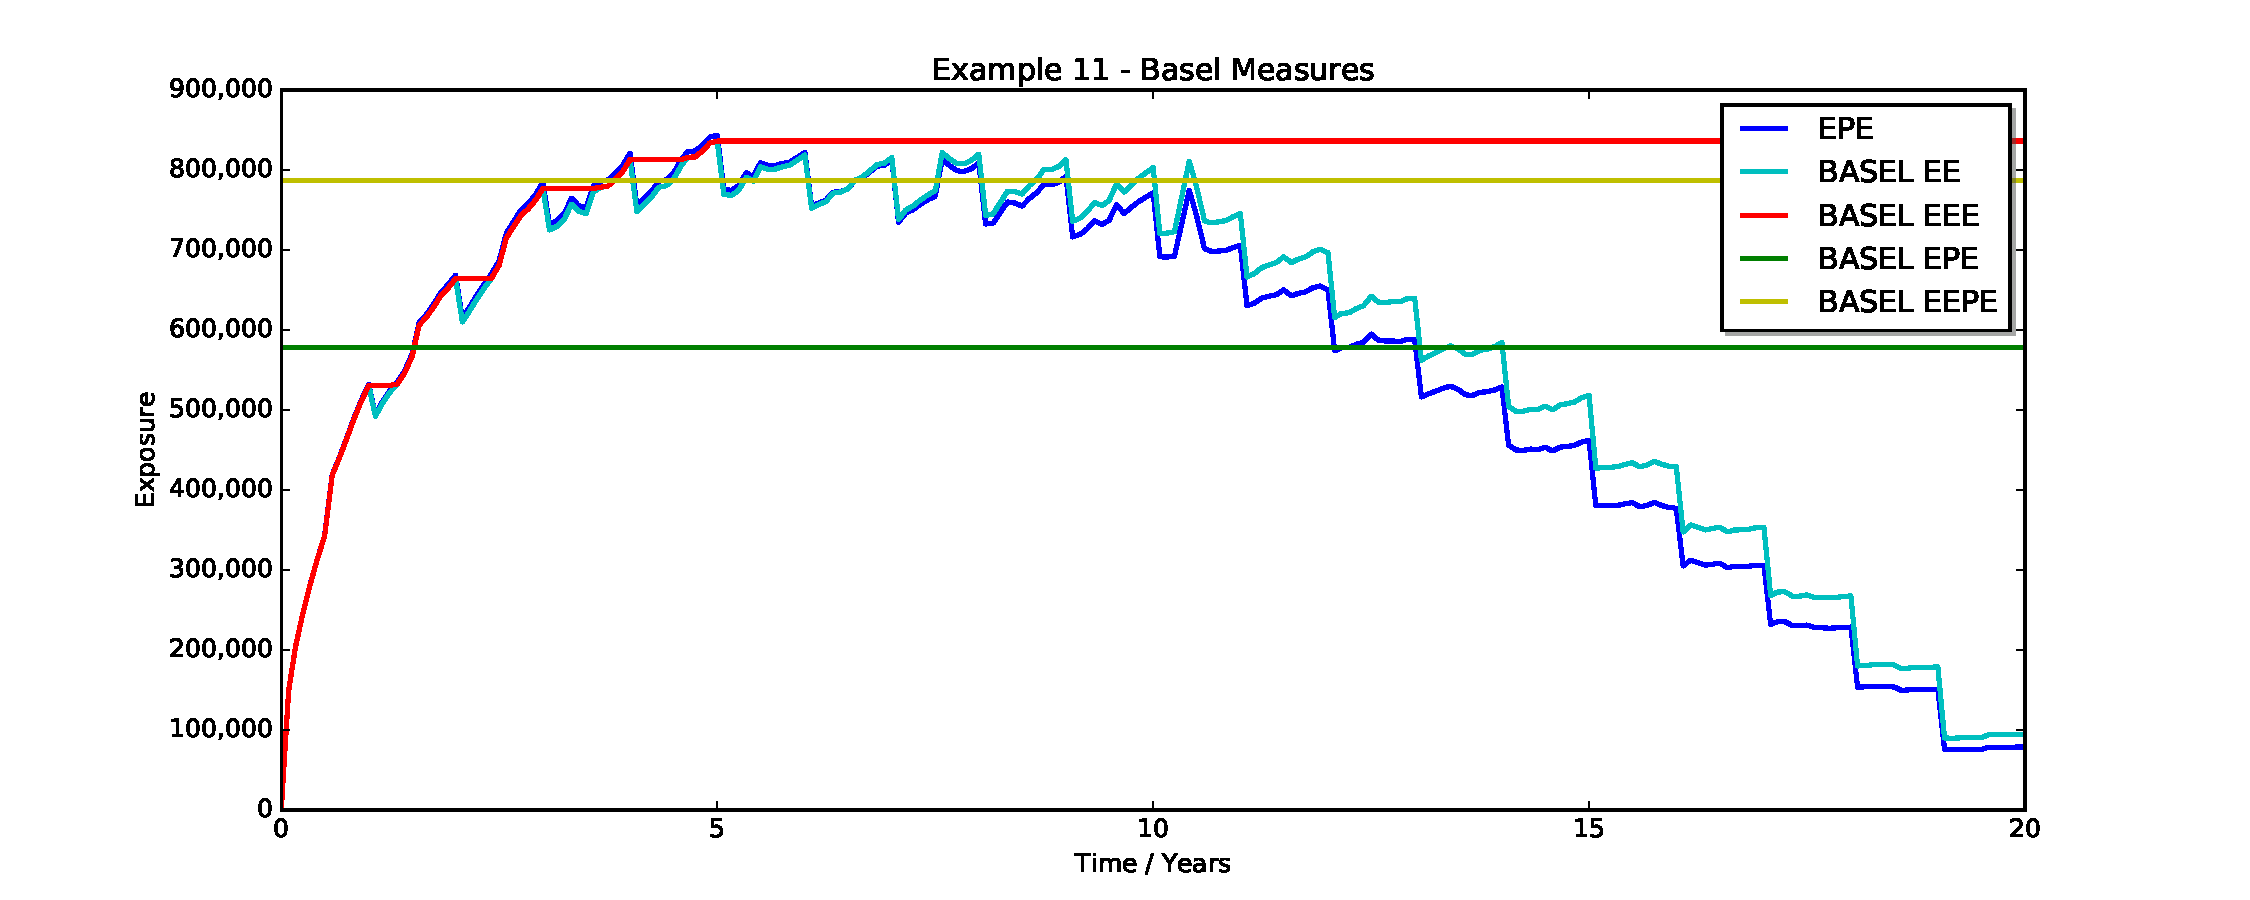
\includegraphics[scale=0.45]{mpl_basel_exposures.pdf}
\end{center}
\caption{Evolution of the expected exposure of Vanilla Swap, comparison to the `Basel' exposure measures EEE\_B, EPE\_B and EEPE\_B.}
\label{fig_14}
\end{figure}

%--------------------------------------------------------
\subsection{Long Term Simulation with Horizon Shift}\label{sec:longterm}
%--------------------------------------------------------

The example in folder {\tt Example\_12} finally demonstrates an effect that, at first glance, seems to cause a serious
issue with long term simulations. Fortunately this can be avoided quite easily in the Linear Gauss Markov model setting
that is used here. \\

In the example we consider a Swap with maturity in 50 years in a flat yield curve environment. If we simulate this
naively as in all previous cases, we obtain a particularly noisy EPE profile that does not nearly reconcile with the
known exposure (analytical Swaption prices). This is shown in figure \ref{fig_15} (`no horizon shift'). The origin of
this issue is the width of the risk-neutral NPV distribution at long time horizons which can turn out to be quite small
so that the Monte Carlo simulation with finite number of samples does not reach far enough into the positive or negative
NPV range to adequately sample the distribution, and estimate both EPE and ENE in a single run.  Increasing the number
of samples may not solve the problem, and may not even be feasible in a realistic setting. \\

The way out is applying a `shift transformation' to the Linear Gauss Markov model, see {\tt
  Example\_12/Input/simulation2.xml} in lines 92-95:
\begin{listing}[H]
%\hrule\medskip
\begin{minted}[fontsize=\footnotesize]{xml}
        <ParameterTransformation>
          <ShiftHorizon>30.0</ShiftHorizon>
          <Scaling>1.0</Scaling>
        </ParameterTransformation>
\end{minted}
%\hrule
%\caption{LGM Shift transformation}
%\label{lst:shift_transformation}
\end{listing}

The effect of the 'ShiftHorizon' parameter $T$ is to apply a shift to the Linear Gauss Markov model's $H(t)$ parameter
(see appendix \ref{sec:app_rfe}) {\em after} the model has been calibrated, i.e. to replace:
$$ 
H(t) \rightarrow H(t) - H(T) 
$$ 
It can be shown that this leaves all expectations computed in the model (such as EPE and ENE) invariant. As explained in
\cite{Lichters}, subtracting a $H$ shift effectively means performing a change of measure from the `native' LGM measure
to a T-Forward measure with horizon $T$, here 30 years. Both negative and positive shifts are permissible, but only
negative shifts are connected with a T-Forward measure and improve numerical stability. \\

In our experience it is helpful to place the horizon in the middle of the portfolio duration to significantly improve
the quality of long term expectations. The effect of this change (only) is shown in the same figure \ref{fig_15}
(`shifted horizon').
\begin{figure}[h!]
\begin{center}
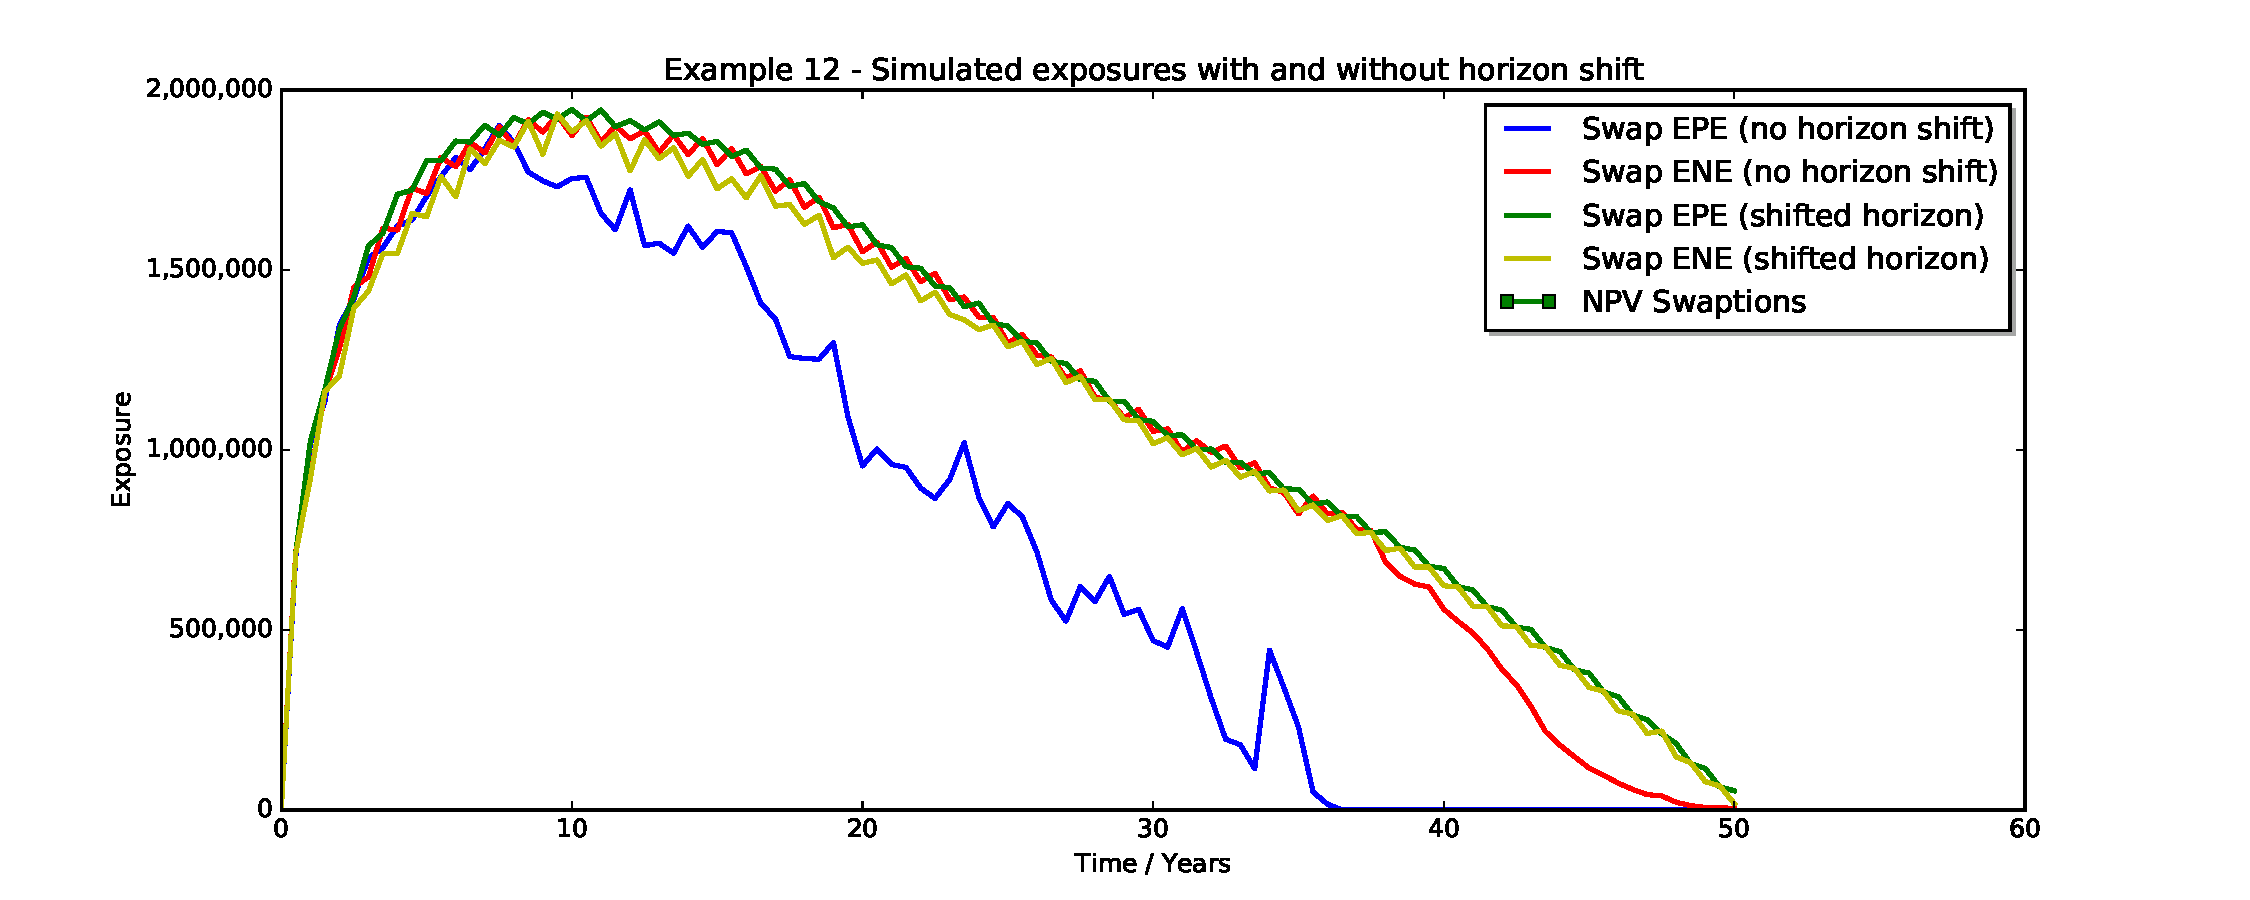
\includegraphics[scale=0.45]{mpl_longterm.pdf}
\end{center}
\caption{Long term Swap exposure simulation with and without horizon shift.}
\label{fig_15}
\end{figure}
Figure \ref{fig_15b} further illustrates the origin of the problem and its resolution: The rate distribution's mean
(without horizon shift or change of measure) drifts upwards due to convexity effects (note that the yield curve is flat
in this example), and the distribution's width is then too narrow at long horizons to yield a sufficient number of low
rate scenarios with contributions to the Swap's $\EPE$ (it is a floating rate payer). With the horizon shift (change of
measure), the distribution's mean is pulled 'back' at long horizons, because the convexity effect is effectively wiped
out at the chosen horizon, and the expected rate matches the forward rate.

\begin{figure}[h!]
\begin{center}
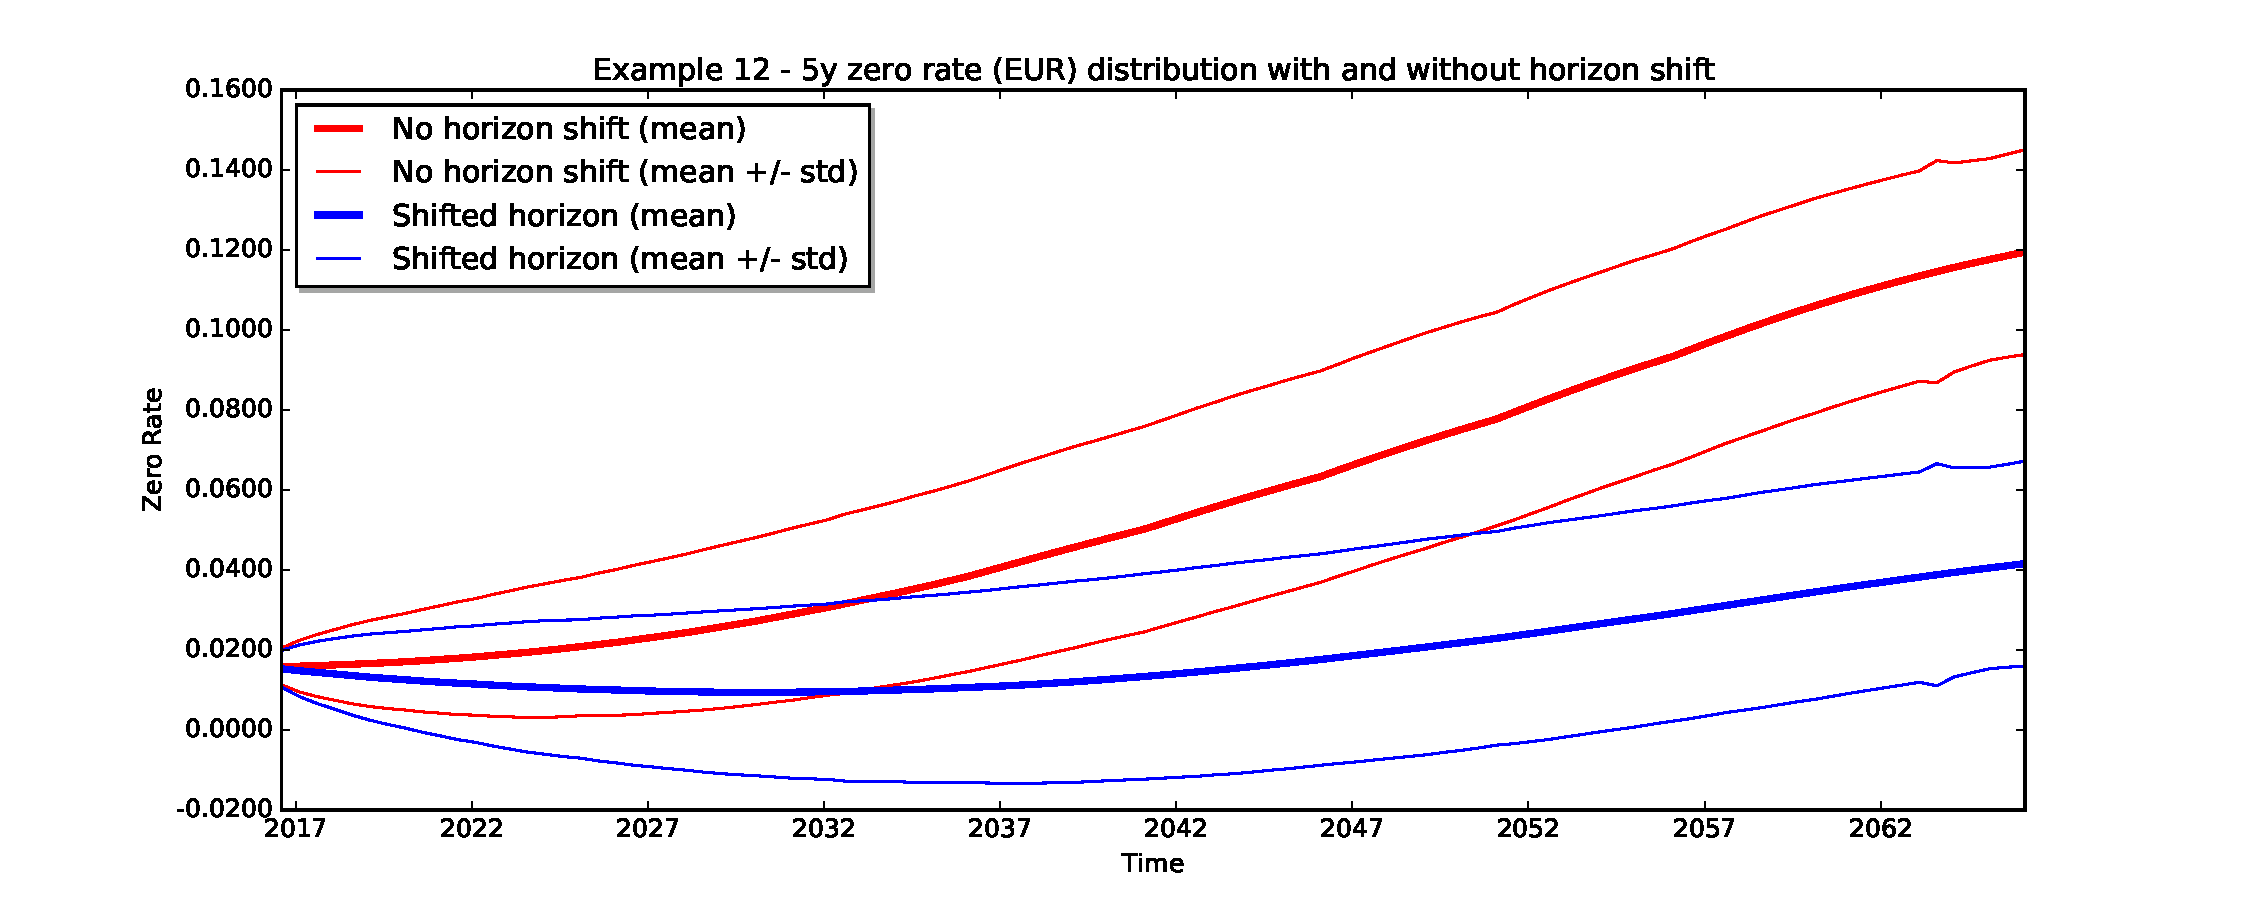
\includegraphics[scale=0.45]{mpl_rates.pdf}
\end{center}
\caption{Evolution of rate distributions with and without horizon shift (change of measure). Thick lines indicate mean
  values, thin lines are contours of the rate distribution at $\pm$ one standard devation.}
\label{fig_15b}
\end{figure}

%--------------------------------------------------------
\subsection{Dynamic Initial Margin and MVA}\label{sec:dim}
%--------------------------------------------------------

This example in folder {\tt Examples/Example\_13} demonstrates Dynamic Initial Margin calculations (see also appendix
\ref{sec:app_dim}) for a number of elementary products:
\begin{itemize}
\item A single currency Swap in EUR (case A), 
\item a European Swaption in EUR with physical delivery (case B), 
\item a single currency Swap in USD (case C), and 
\item a EUR/USD cross currency Swap (case D).
\end{itemize}

The examples can be run as before with 

\medskip
\centerline{\tt python run\_A.py} 

\medskip
and likewise for cases B, C and D. The essential results of each run are are visualised in the form of 
\begin{itemize}
\item evolution of expected DIM
\item regression plots at selected future times 
\end{itemize}
illustrated for cases A and B in figures \ref{fig_ex13a_evolution} - \ref{fig_ex13b_regression}. In all cases the zero
order regression estimate of DIM differs noticeably from the higher orders (one and two). In the three swap cases we
moreover see that first and second order polynomial choice makes hardly any difference; note that case C and D use up to
three-dimensional regressors (simulated USD and EUR rate fixings and the EUR/USD FX rate). In the Swaption case B, first
and second order polynomial choice makes a difference before option expiry. More details on this DIM model and its performance can be found in \cite{Anfuso2016,LichtersEtAl}.
 
\begin{figure}[h!]
\begin{center}
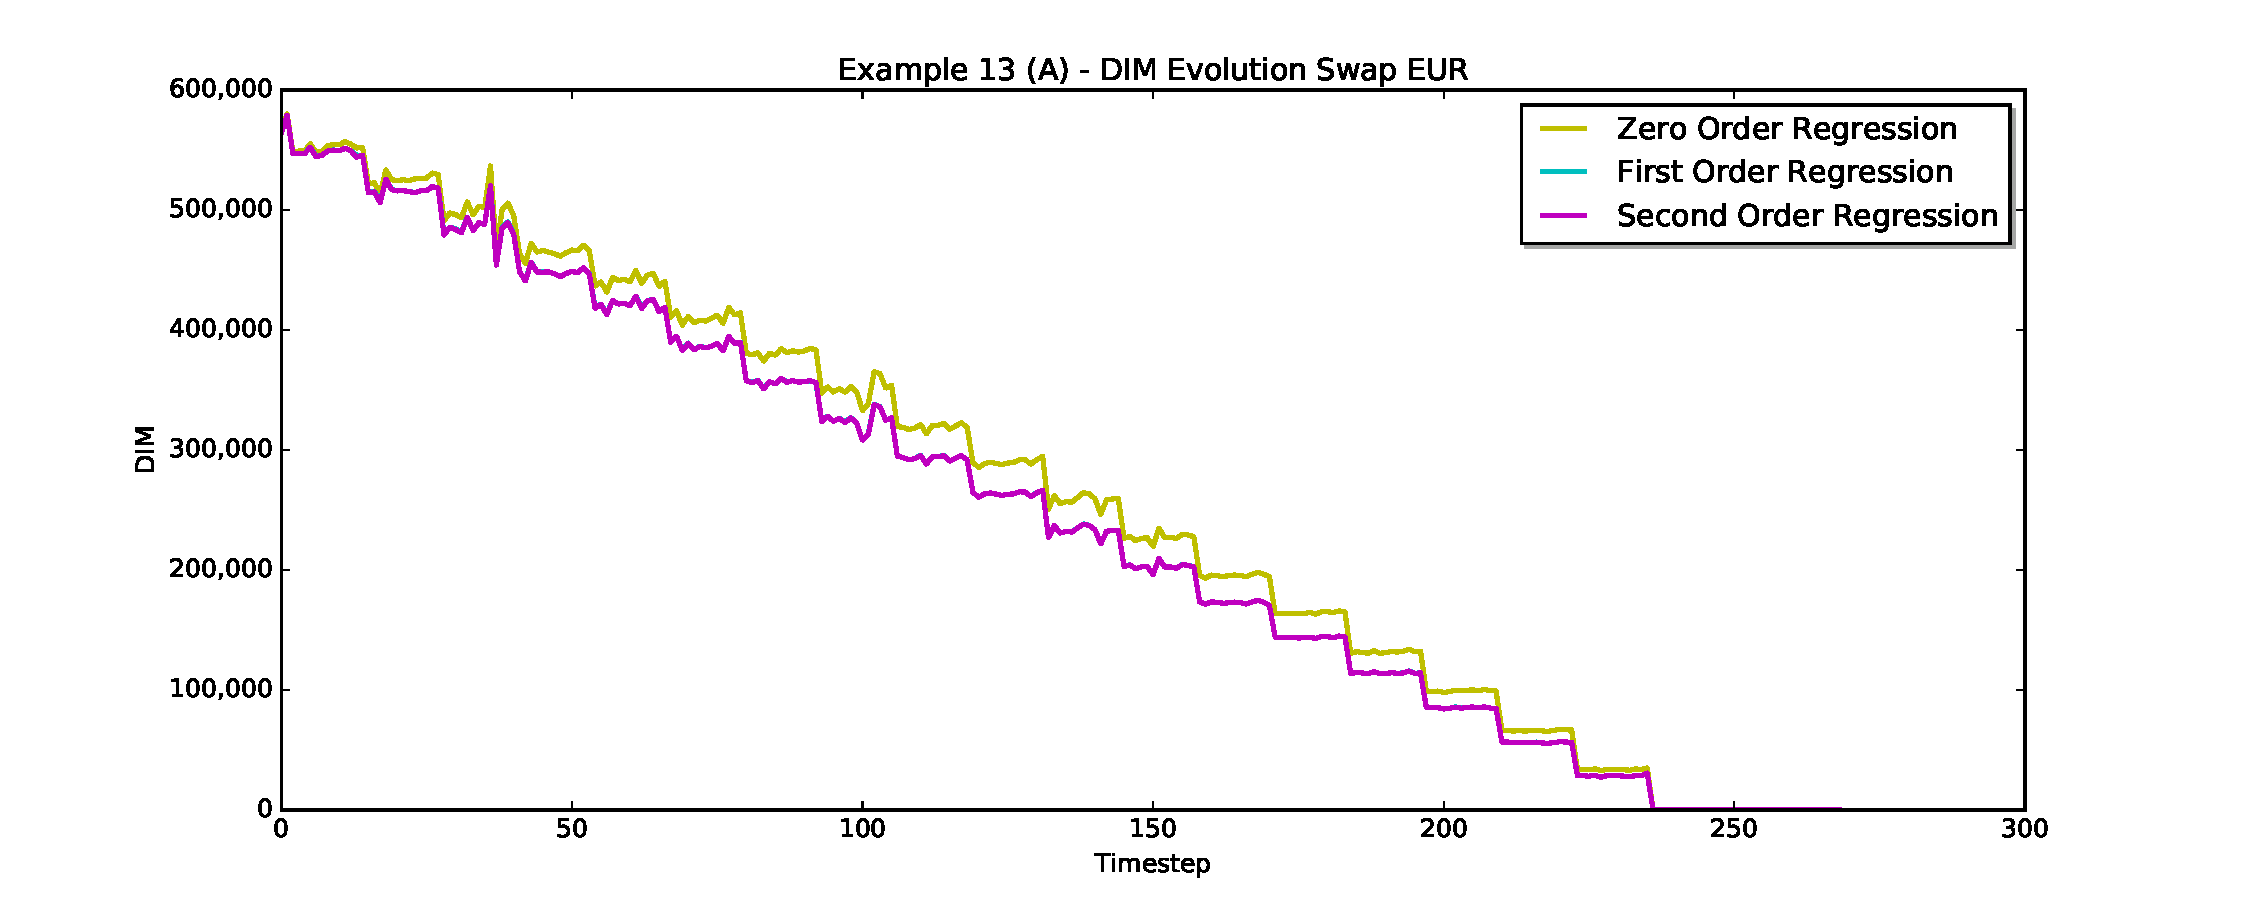
\includegraphics[scale=0.45]{mpl_dim_evolution_A_swap_eur.pdf}
\end{center}
\caption{Evolution of expected Dynamic Initial Margin (DIM) for the EUR Swap of Example 13 A. DIM is evaluated using
  regression of NPV change variances versus the simulated 3M Euribor fixing; regression polynomials are zero, first and
  second order (first and second order curves are not distinguishable here). The simulation uses 1000 samples and a time
  grid with bi-weekly steps in line with the Margin Period of Risk.}
\label{fig_ex13a_evolution}
\end{figure}

\begin{figure}[h!]
\begin{center}
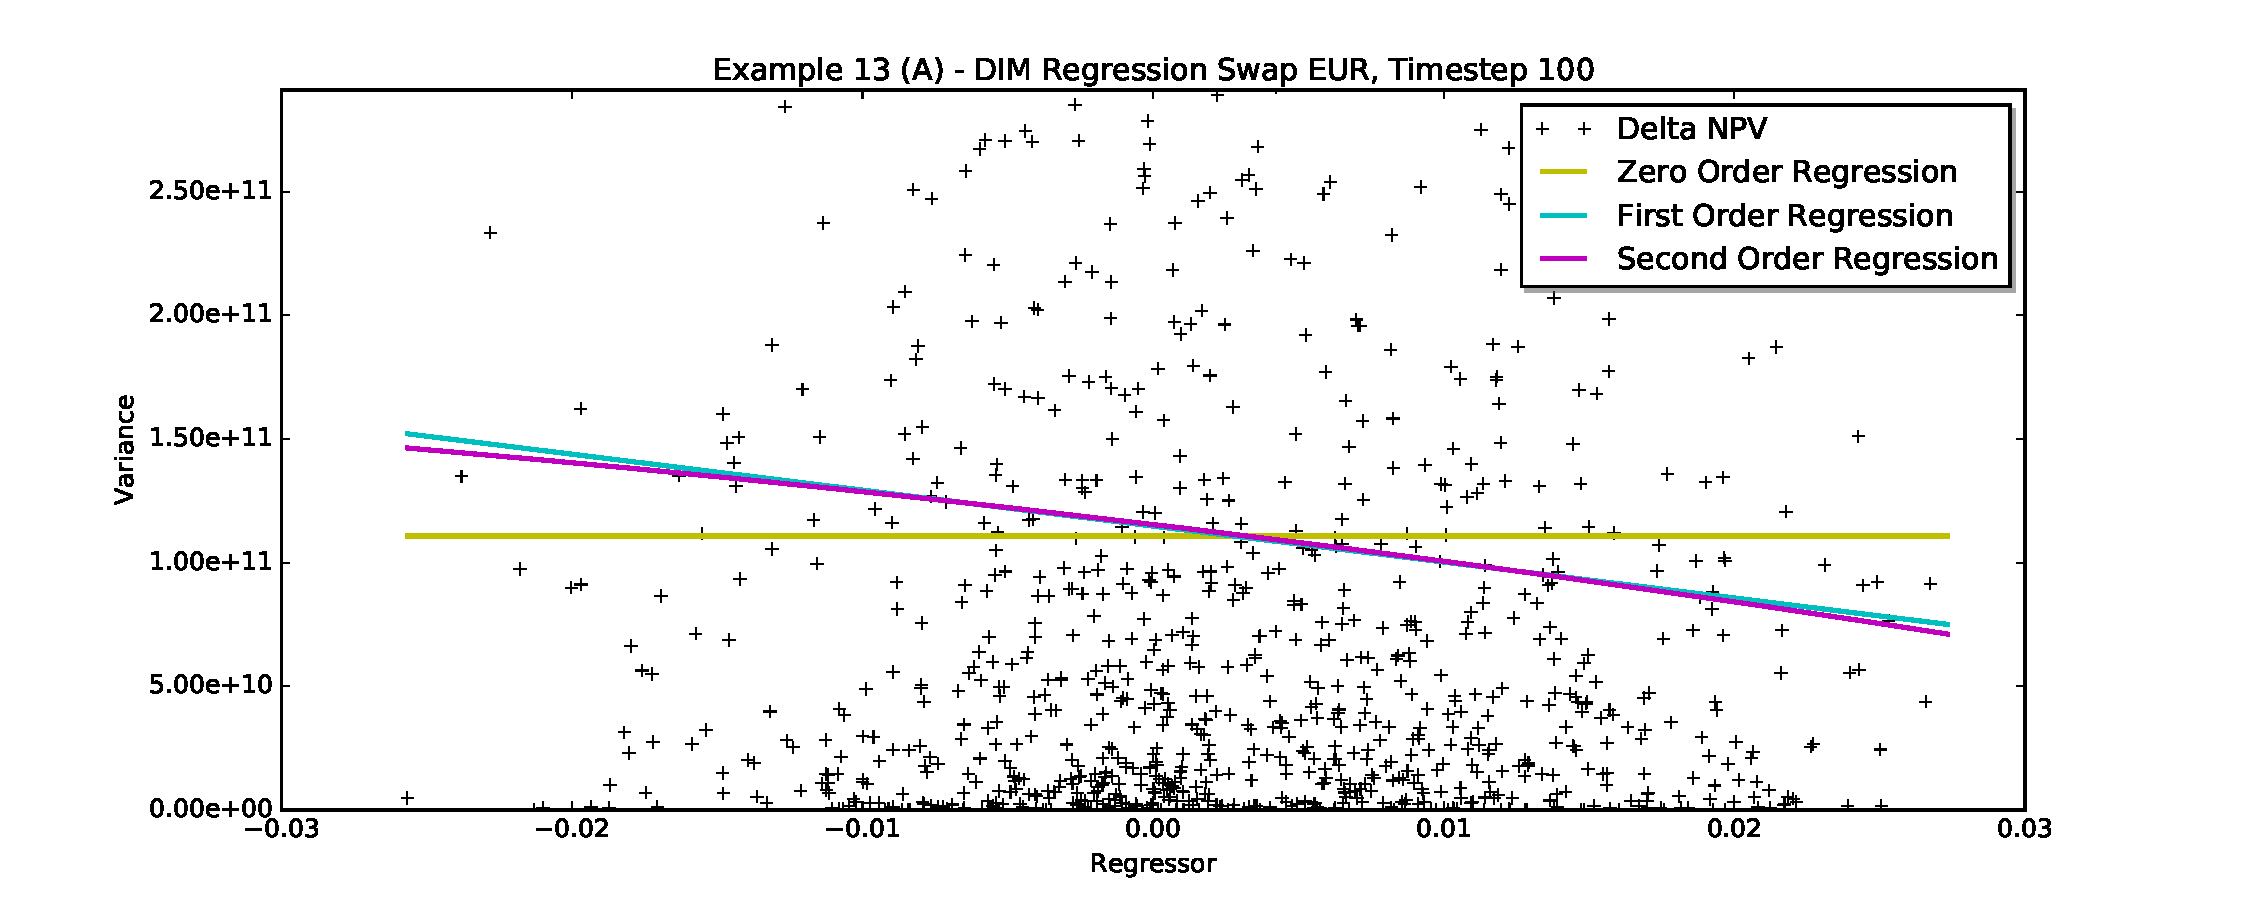
\includegraphics[scale=0.45]{mpl_dim_regression_A_swap_eur.pdf}
\end{center}
\caption{Regression snapshot at time step 100 for the EUR Swap of Example 13 A.}
\label{fig_ex13a_regression}
\end{figure}

\begin{figure}[h!]
\begin{center}
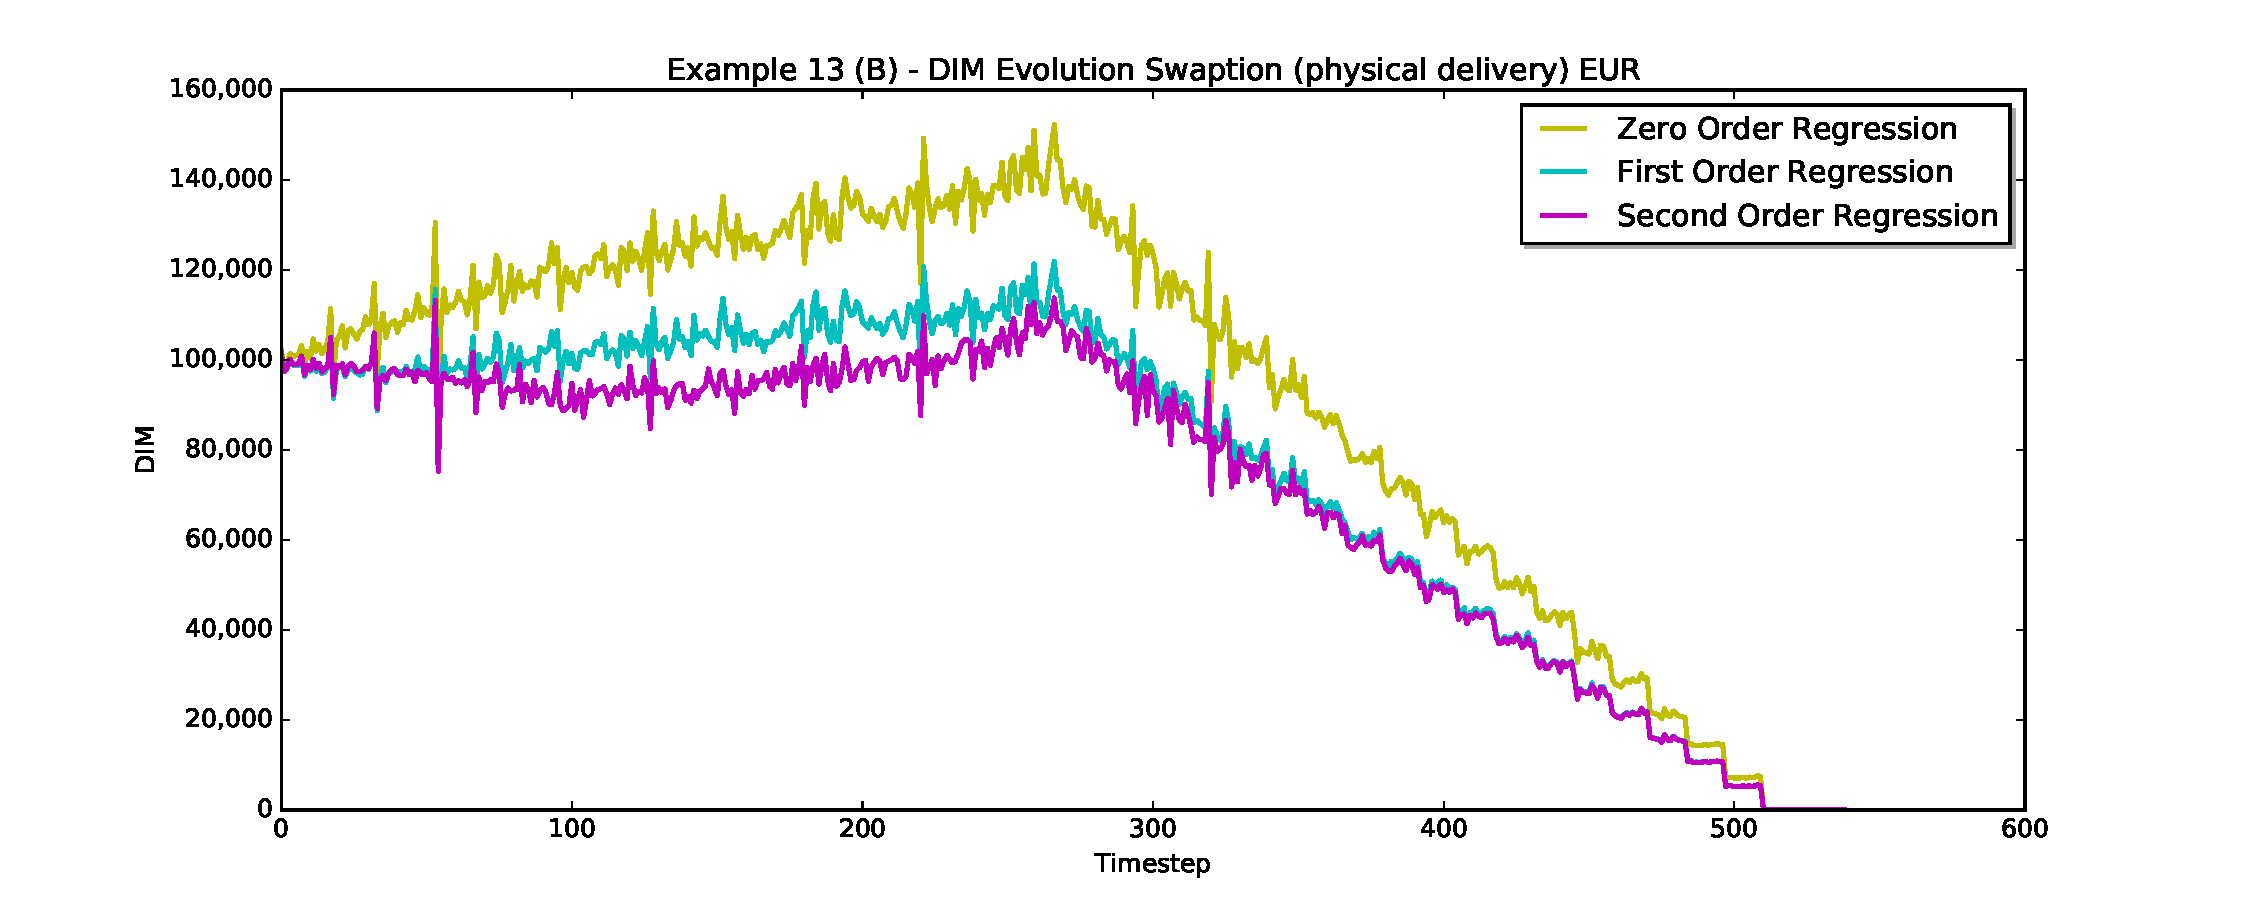
\includegraphics[scale=0.45]{mpl_dim_evolution_B_swaption_eur.pdf}
\end{center}
\caption{Evolution of expected Dynamic Initial Margin (DIM) for the EUR Swaption of Example 13 B with expiry in 10Y
  around time step 100. DIM is evaluated using regression of NPV change variances versus the simulated 3M Euribor
  fixing; regression polynomials are zero, first and second order. The simulation uses 1000 samples and a time grid with
  bi-weekly steps in line with the Margin Period of Risk.}
\label{fig_ex13b_evolution}
\end{figure}

\begin{figure}[h!]
\begin{center}
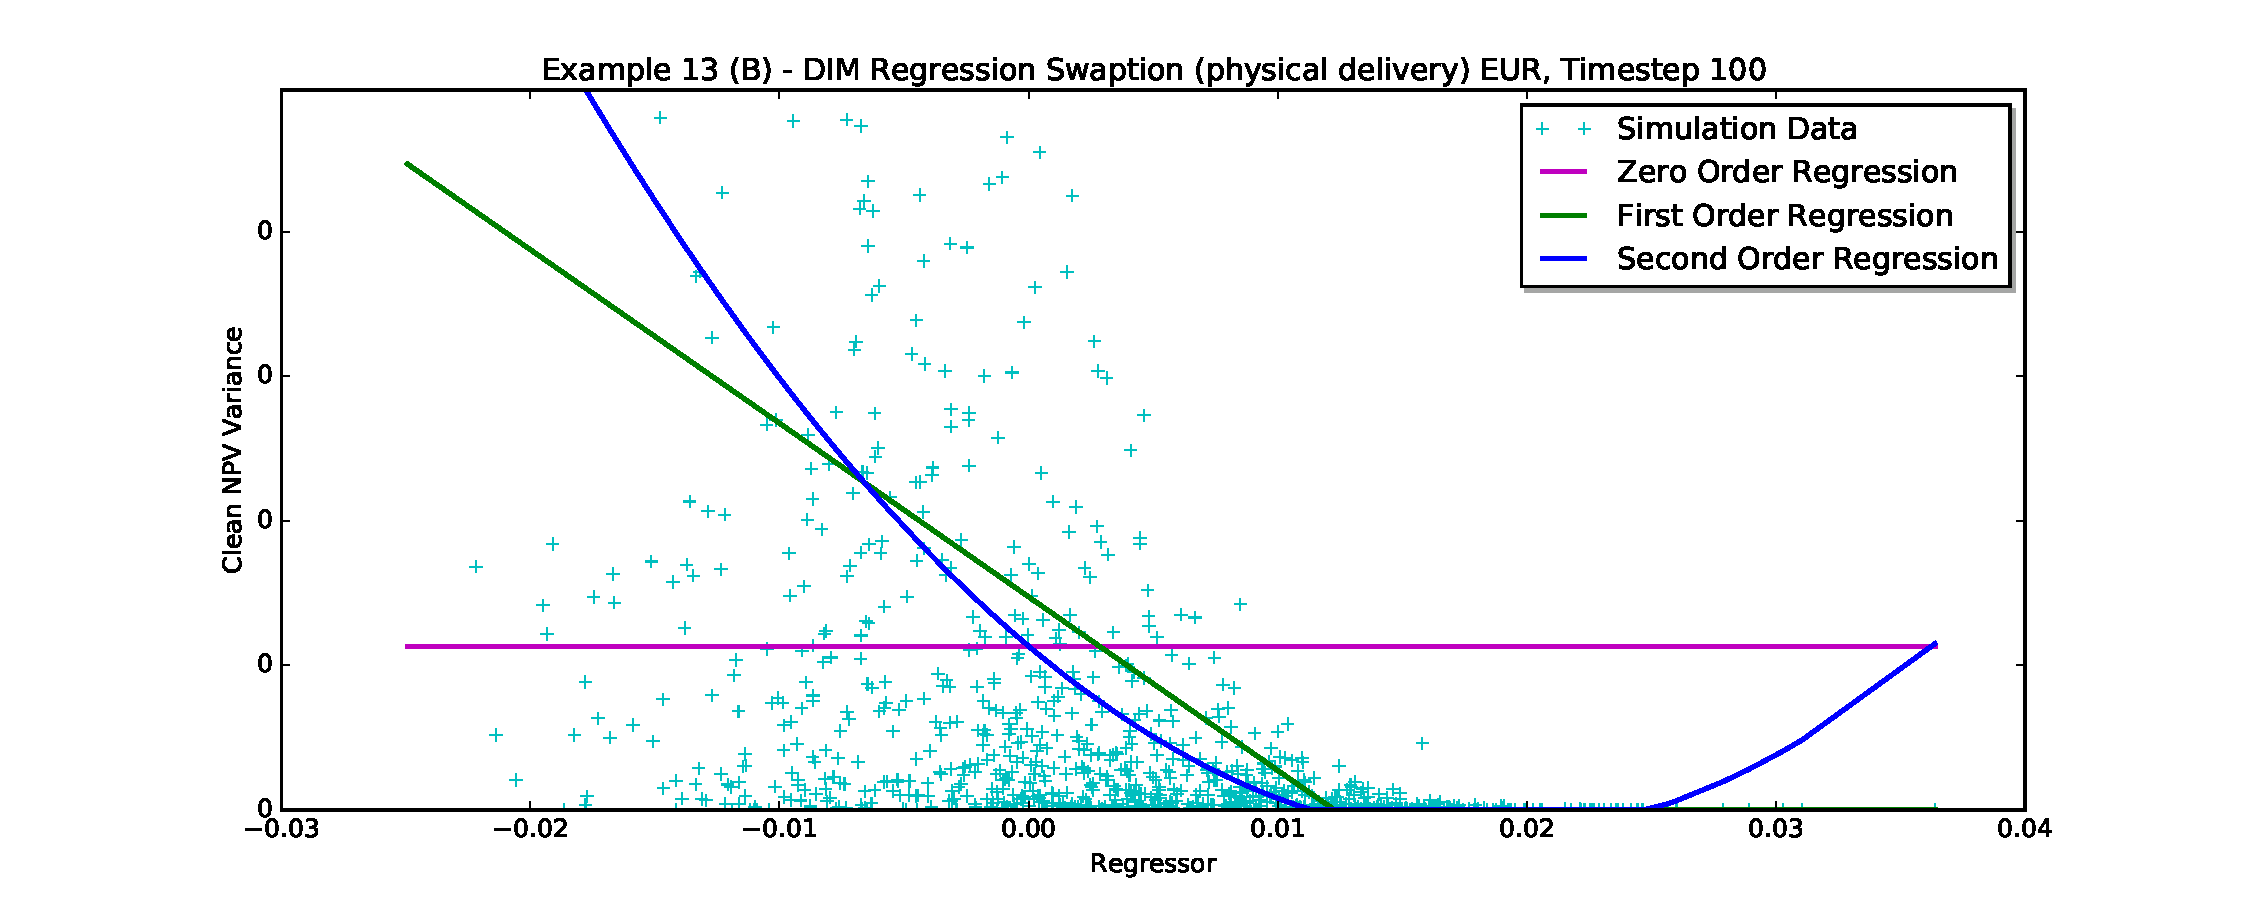
\includegraphics[scale=0.45]{mpl_dim_regression_B_swaption_eur_t100.pdf}
\end{center}
\caption{Regression snapshot at time step 100 (before expiry) for the EUR Swaption of Example 13 B.}
\label{fig_ex13b_regression}
\end{figure}

%--------------------------------------------------------
\subsection{Minimal Market Data Setup}
%--------------------------------------------------------

The example in folder {\tt Examples/Example\_14} demonstrates using a minimal market data setup in order to rerun the vanilla Swap exposure simulation shown in {\tt Examples/Example\_1}. The minimal market data uses single points per curve where possible.

%--------------------------------------------------------
\subsection{Sensitivity Analysis and Stress Testing}\label{ex:sensitivity_stress}
%--------------------------------------------------------

The example in folder {\tt Examples/Example\_15} demonstrates the calculation of sensitivities and stress scenarios. The
portfolio used in this example consists of

\begin{itemize}
\item a vanilla swap in EUR
\item a cross currency swap EUR-USD
\item a resettable cross currency swap EUR-USD
\item a FX forward EUR-USD
\item a FX call option
\item a FX put option
\item an European swaption
\item a cap in USD
\item a floor in USD
\item a cap in EUR
\item a floor in UER
\item a fixed rate bond
\end{itemize}

The sensitivity configuration in {\tt sensitivity.xml} aims at computing the following sensitivities

\begin{itemize}
\item discount curve sensitivities in EUR, USD; GBP, CHF, JPY, on pillars 6M, 1Y, 2Y, 3Y, 5Y, 7Y, 10Y, 15Y, 20Y (absolute shift of 0.0001)
\item forward curve sensitivities for EUR-EURIBOR 6M and 3M indices, EUR-EONIA, USD-LIBOR 3M and 6M, GBP-LIBOR 3M and
  6M, CHF-LIBOR-6M and JPY-LIBOR-6M indices (absolute shift of 0.0001)
\item yield curve shifts for a bond benchmark curve in EUR (absolute shift of 0.0001)
\item FX spot sensitivities for USD, GBP, CHF, JPY against EUR as the base currency (relative shift of 0.01)
\item FX vegas for USDEUR, GBPEUR, JPYEUR volatility surfaces (relative shift of 0.01)
\item swaption vegas for the EUR surface on expiries 1Y, 5Y, 7Y, 10Y and underlying terms 1Y, 5Y, 10Y (relative shift of 0.01)
\item caplet vegas for EUR and USD on an expiry grid 1Y, 2Y, 3Y, 5Y, 7Y, 10Y and strikes 0.01, 0.02, 0.03, 0.04,
  0.05. (absolute shift of 0.0001)
\end{itemize}

Furthermore, mixed second order derivatives (``cross gammas'') are computed for discount-discount, discount-forward and
forward-forward curves in EUR.

By definition the sensitivities are zero rate sensitivities and optionlet sensitivities, no par sensitivities are
provided. The sensitivity analysis produces three output files.

The first, {\tt scenario.csv}, contains the shift
direction ({\tt UP}, {\tt DOWN}, {\tt CROSS}), the base NPV, the scenario NPV and the difference of these two for each
trade and sensitivity key. For an overview over the possible scenario keys see \ref{sec:sensitivity}.

The second file, {\tt sensitivity.csv}, contains the shift size (in absolute terms always) and first (``Delta'') and second
(``Gamma'') order finite differences computed from the scenario results. Note that the Delta and Gamma results pure
differences, i.e. they are not divided by the shift size.

The third file, {\tt crossgamma.csv} contains second order mixed differences according to the specified cross gamma
filter, along with the shift sizes for the two factors involved. Again the reported result is not divided by the shift
sizes.

The stress scenario definition in {\tt stresstest.xml} defines two stress tests:

\begin{itemize}
\item {\tt parallel\_rates}: Rates are shifted in parallel by 0.01 (absolute). The EUR bond benchmark curve is shifted by
  increasing amounts 0.001, ..., 0.009 on the pillars 6M, ..., 20Y. FX Spots are shifted by 0.01 (relative), FX vols by
  0.1 (relative), swaption and cap floor vols by 0.0010 (absolute)
\item {\tt twist}: The EUR bond benchmark curve is shifted by amounts -0.0050, -0.0040, -0.0030, -0.0020, 0.0020,
  0.0040, 0.0060, 0.0080, 0.0100 on pillars 6M, 1Y, 2Y, 3Y, 5Y, 7Y, 10Y, 15Y, 20Y.
\end{itemize}

The corresponding output file {\tt stresstest.csv} contains the base NPV, the NPV under the scenario shifts and the
difference of the two for each trade and scenario label.

\todo[inline]{Update after CDS has been added to the example.}

%--------------------------------------------------------
\subsection{Equity Derivatives Exposure}\label{ex:equityderivatives}
%--------------------------------------------------------

The example in folder {\tt Examples/Example\_16} demonstrates the computation of NPV, exposures and XVA for a portfolio 
of OTC equity derivatives. The portfolio used in this example consists of:

\begin{itemize}
	\item an equity call option denominated in EUR (``Luft'')
	\item an equity put option denominated in EUR (``Luft'')
	\item an equity forward denominated in EUR (``Luft'')
	\item an equity call option denominated in USD (``SP5'')
	\item an equity put option denominated in USD (``SP5'')
	\item an equity forward denominated in USD (``SP5'')
\end{itemize}

The step-by-step procedure for running ORE is identical for equities as for other asset classes; the same market and 
portfolio data files are used to store the equity market data and trade details, respectively. For the exposure 
simulation, the calibration parameters for the equity risk factors can be set in the usual {\tt simulation.xml} file.

Looking at the MtM results in the output file {\tt npv.csv} we observe that put-call parity ($V_{Fwd} = V_{Call} - 
V_{Put}$) is observed as expected. Looking at Figure \ref{fig_eq_call} we observe that the Expected Exposure profile of 
the equity call option trade is relatively smooth over time, while for the equity forward trade the Expected Exposure 
tends to increase as we approach maturity. This behaviour is similar to what we observe in sections \ref{sec:fxfwd} 
and \ref{sec:fxoption}. 

\begin{figure}[h!]
	\begin{center}
		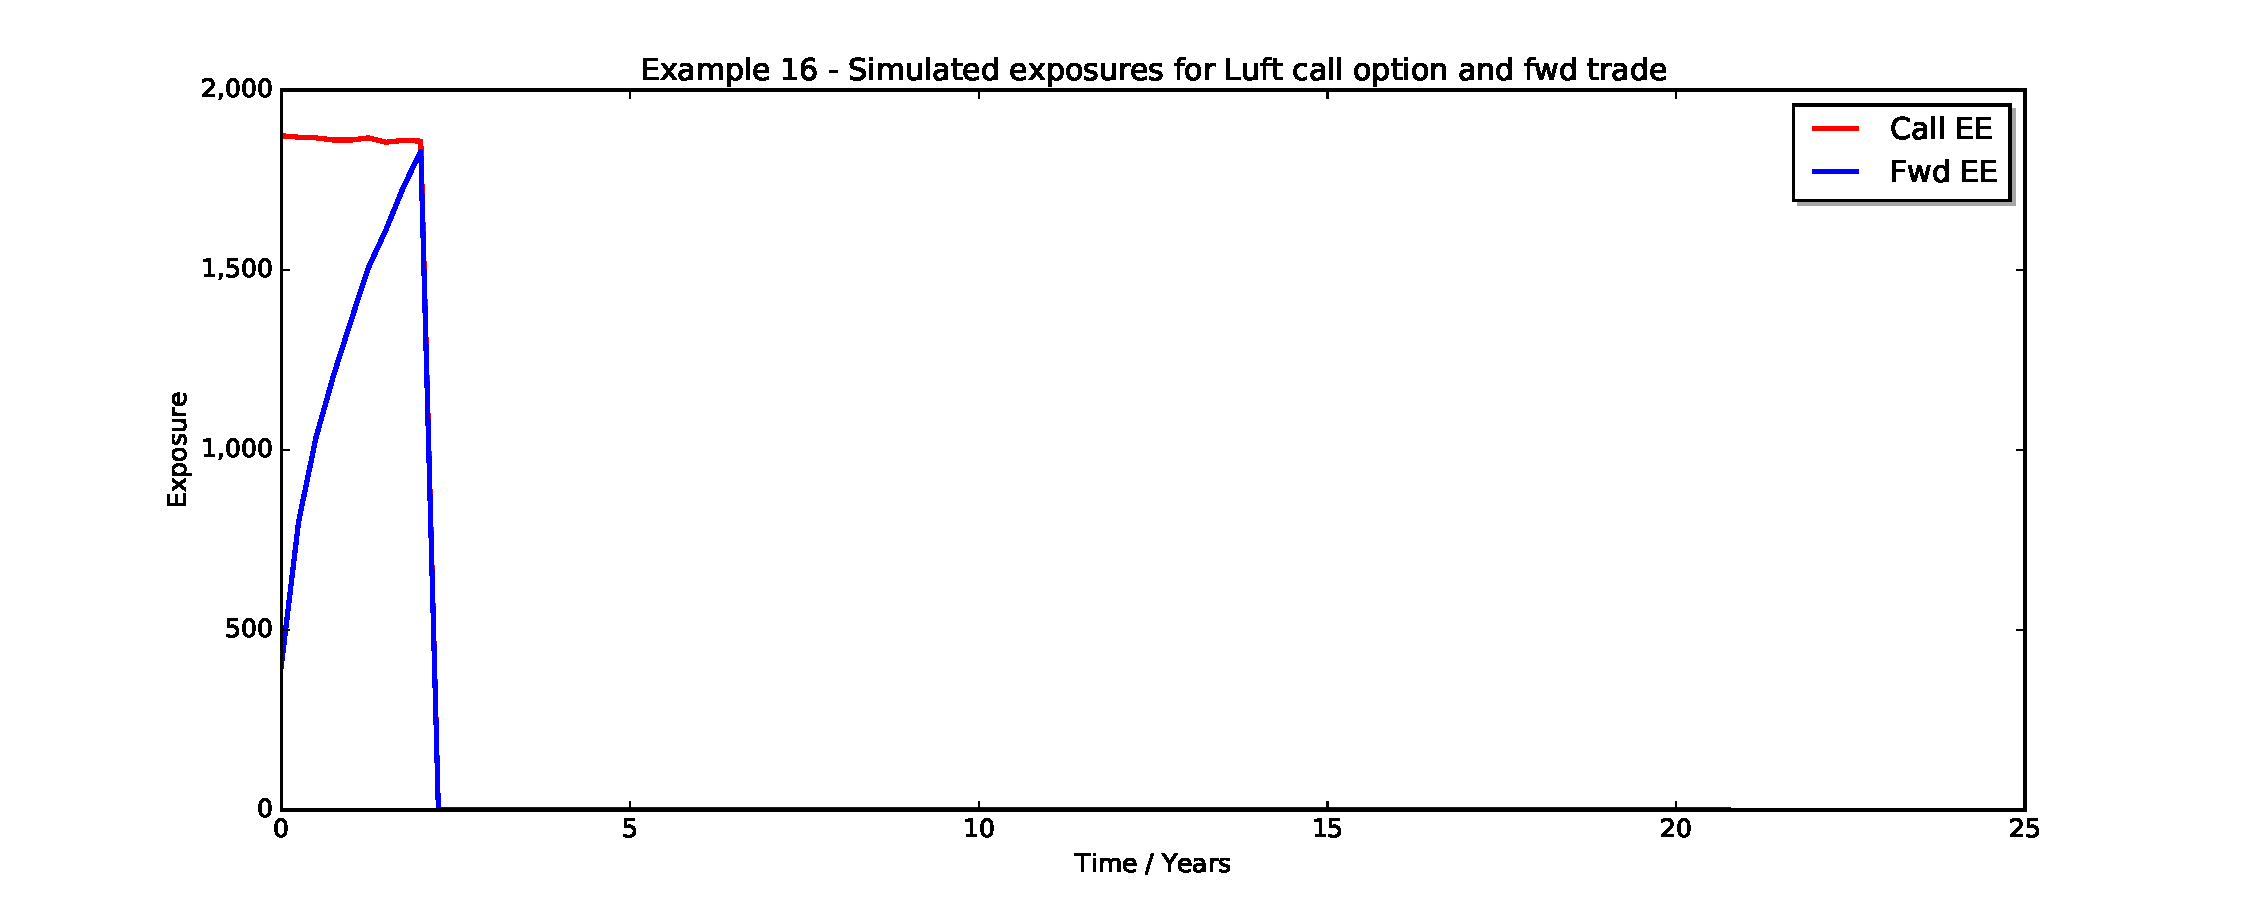
\includegraphics[scale=0.45]{mpl_eq_call.pdf}
	\end{center}
	\caption{Equity (``Luft'') call option and OTC forward exposure evolution, maturity in approximately 2.5 years. 
	Simulation with 
	10000 paths and quarterly time steps.}
	\label{fig_eq_call}
\end{figure}

%--------------------------------------------------------
\subsection{Inflation Swaps}
%--------------------------------------------------------

The example in folder {\tt Examples/Example\_17} computes the NPV of a CPI Swap and a Year on Year Swap. The terms of
the two deals are as follows, CPI Swap:

\begin{itemize}
\item Start 2016-07-18, Maturity 2021-07-18
\item GBP Libor 6M vs. $2\%$ x CPI-Factor (Act/Act), with
\item CPI-Factor = UKRPI fixing with an observation lag of 2M divided by the base CPI value 210, inflation fixing is not
  interpolated
\end{itemize}

Year on Year Swap:

\begin{itemize}
\item Start 2016-07-18, Maturity 2021-07-18
\item EUR Euribor 6M vs. Year on Year payoff (Act/Act) on EUHICPXT, inflation fixings are observed with a lag of 2M,
  include 2 fixing days, and are interpolated
\end{itemize}

After running the example, the results of the computation can be found in the output file {\tt npv.csv}.

\todo[inline]{Merge new inflation exposure example 24 into example 17}

%--------------------------------------------------------
\subsection{Bonds and Amortisation Structures}
%--------------------------------------------------------

The example in folder {\tt Examples/Example\_18} computes NPVs and cash flow projections for a vanilla bond portfolio
consisting of a range of bond products, in particular demonstrating amortisation features:
\begin{itemize}
\item fixed rate bond
\item floating rate bond linked to Euribor 6M
\item bond switching from fixed to floating
\item bond with 'fixed amount' amortisation
\item bond with percentage amortisation relative to the initial notional
\item bond with percentage amortisation relative to the previous notional
\item bond with fixed annuity amortisation
\item bond with floating annuity amortisation (this example needs QuantLib 1.10 or higher to work, in particular the amount() method in the Coupon class needs to be virtual)
\item bond with fixed amount amortisation followed by percentage amortisation relative to previous notional
\end{itemize}

After running the example, the results of the computation can be found in the output files {\tt npv.csv} and {\tt
  flows.csv}, respectively.

\medskip
Note that the amortisation features used here are linked to the LegData structure, hence not limited to the Bond instrument, see section \ref{ss:amortisationdata}.

%--------------------------------------------------------
\subsection{Swaption Pricing with Smile}% Example 19
%--------------------------------------------------------

This example in folder {\tt Examples/Example\_19} demonstrates European Swaption pricing with and without smile. Calling

\medskip
\centerline{\tt python run.py}

\medskip
will launch two ORE runs using config files {\tt ore\_flat.xml} and {\tt ore\_smile.xml}, respectively. The only difference in these is referencing alternative market configurations {\tt todaymarket\_flat.xml} and {\tt todaysmarket\_smile.xml} using an ATM Swaption volatility matrix and a Swaption cube, respectively. NPV results are written to {\tt npv\_flat.cvs} and {\tt npv\_smile.csv}.

%--------------------------------------------------------
\subsection{Credit Default Swap Pricing}% Example 20
%--------------------------------------------------------

This example in folder {\tt Examples/Example\_20} demonstrates Credit Default Swap pricing via ORE. Calling

\medskip
\centerline{\tt python run.py}

\medskip
will launch a single ORE run to process a single name CDS example and to generate NPV and cash flows in the usual result files. 

\medskip
CDS can be included in sensitivity analysis and stress testing. Exposure simulation for credit derivatives will follow in the next ORE release.

%--------------------------------------------------------
\subsection{CMS and CMS Cap/Floor Pricing}% Example 21
%--------------------------------------------------------

This example in folder {\tt Examples/Example\_21} demonstrates the pricing of CMS and CMS Cap/Floor using a portfolio consisting of a CMS Swap (CMS leg vs. fixed leg) and a CMS Cap. Calling

\medskip
\centerline{\tt python run.py}

\medskip
will launch a single ORE run to process the portfolio and generate NPV and cash flows in the usual result files. 

\medskip
CMS structures can be included in sensitivity analysis, stress testing and exposure simulation. 

%--------------------------------------------------------
\subsection{Option Sensitivity Analysis with Smile}% Example 22
%--------------------------------------------------------

The example in folder {\tt Examples/Example\_22} demonstrates the calculation of sensitivities for European swaptions and equity options where the volatility surface has a smile. 

\medskip
The portfolio used in this example consists of:
\begin{itemize}
	\item an equity call option denominated in USD (``SP5'')
	\item an equity put option denominated in USD (``SP5'')
	\item a receiver swaption in EUR
\end{itemize}

\medskip
ORE supports two methods of simulating equity volatility smile. The first method simulates the entire surface using specific moneyness levels configured in simulation.xml. The second method simulates only the ATM equity volatilities, the other strikes are shifted relative to this new ATM using the $t_{0}$ smile.  This example compares both methods using the same sensitivity configuration as in {\tt Examples/Example\_15}. For the first method {\tt simulation\_fullSurface.xml} is used and all output files are appended with ``\_fullSurface'', for the second method {\tt simulation\_atmOnly.xml} is used and all output files are appended with ``\_atmOnly''.

\todo[inline]{Update this section once example 22 has been reviewed}

%--------------------------------------------------------
\subsection{FRA and Average OIS Exposure}% Example 23
%--------------------------------------------------------

This example in folder {\tt Examples/Example\_23} demonstrates pricing, cash flow projection and exposure simulation for two additional products
\begin{itemize}
\item Forward Rate Agreements
\item Averaging Overnight Index Swaps
\end{itemize}
using a minimal portfolio of four trades, one FRA and three OIS. The essential results are in {\tt npv.csv}, {\tt flows.csv} and 
four {\tt exposure\_trade\_*.csv} files.

\clearpage
%========================================================
\section{Launchers and Visualisation}\label{sec:visualisation}
%========================================================

\subsection{Jupyter}\label{sec:jupyter}

ORE comes with an experimental Jupyter notebook for launching ORE batches and in particular for drilling into NPV cube
data.  The notebook is located in directory {\tt FrontEnd/Python/Visualization/npvcube}. To launch the notebook, change
to this directory and follow instructions in the {\tt Readme.txt}. In a nutshell, type\footnote{With Mac OS X, you may
  need to set the environment variable {\tt LANG} to {\tt en\_US.UTF-8} before running jupyter, as mentioned in the
  installation section \ref{sec:python}.}

\medskip
\centerline{\tt jupyter notebook}
\medskip

to start the ipyton console and open a browser window. From the list of files displayed in the browser then click

\medskip
\centerline{\tt ore\_jupyter\_dashboard.ipynb} 
\medskip

to open the ORE notebook. The notebook offers
\begin{itemize}
\item launching an ORE job
\item selecting an NPV cube file and netting sets or trades therein
\item plotting a 3d exposure probability density surface
\item viewing exposure probability density function at a selected future time
\item viewing expected exposure evolution through time  
\end{itemize}

The cube file loaded here by default when processing all cells of the notebook (without changing it or launching a ORE
batch) is taken from {\tt Example\_7} (FX Forwards and FX Options).

%\todo[inline]{Add Jupyter section}

\subsection{Calc}\label{sec:calc}

ORE comes with a simple LibreOffice Calc \cite{LO} sheet as an ORE launcher and basic result viewer. This is
demonstrated on the example in section \ref{sec:example1}. It is currently based on the stable LibreOffice version 5.0.6
and tested on OS X. \\

To launch Calc, open a terminal, change to directory {\tt Examples/Example\_1}, and run

\medskip
{\centerline{\tt ./launchCalc.sh} }
\medskip

%This will show the blank sheet in figure \ref{fig_14}.
%\begin{figure}[h]
%\begin{center}
%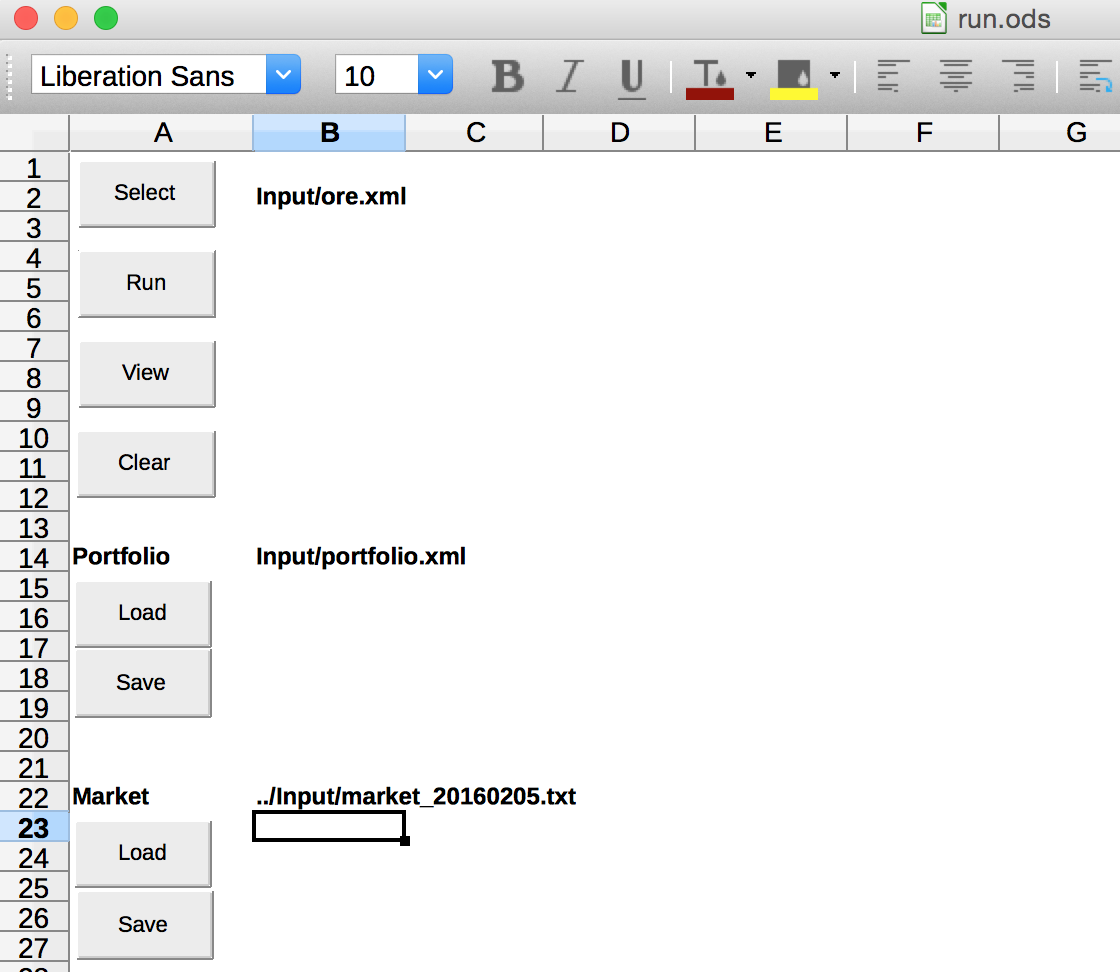
\includegraphics[scale=0.4]{demo_calc_1}
%\end{center}
%\caption{Calc sheet after launching.}
%\label{fig_14}
%\end{figure}
The user can choose a configuration (one of the {\tt ore*.xml} files in Example\_1's subfolder Input) by hitting the
'Select' button. Initially Input/ore.xml is pre-selected. The ORE process is then kicked off by hitting 'Run'. Once
completed, standard ORE reports (NPV, Cashflow, XVA) are loaded into several sheets. Moreover, exposure evolutions can
then be viewed by hitting 'View' which shows the result in figure \ref{fig_16}.  \\
\begin{figure}[h]
\begin{center}
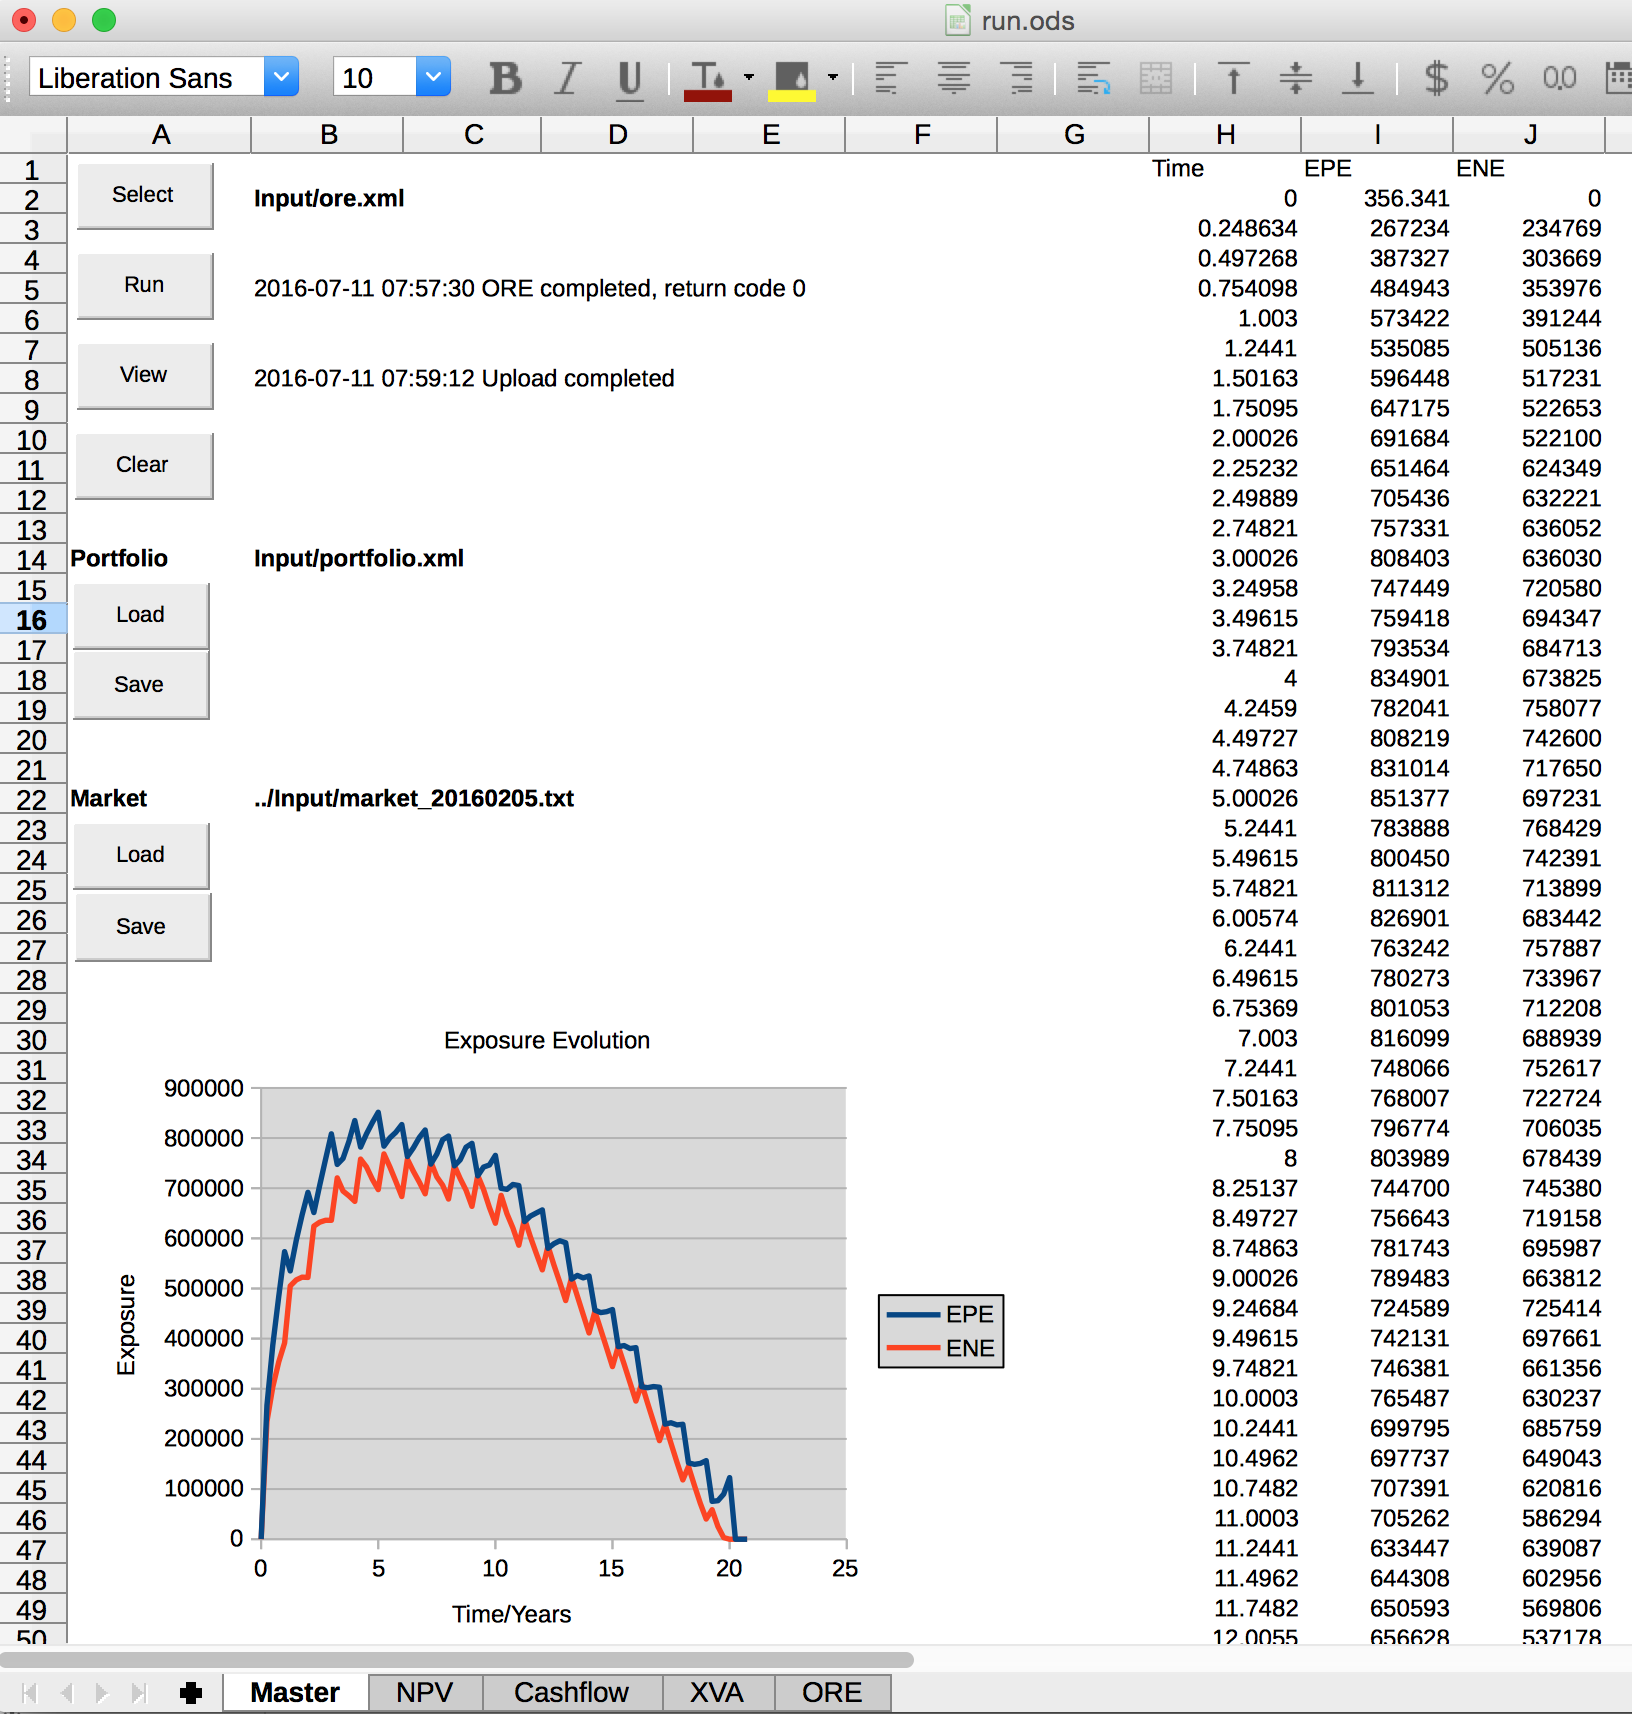
\includegraphics[scale=0.4]{demo_calc_2}
\end{center}
\caption{Calc sheet after hitting 'Run'.}
\label{fig_16}
\end{figure}

This demo uses simple Libre Office Basic macros which call Python scripts to execute ORE. The Libre Office Python uno
module (which comes with Libre Office) is used to communicate between Python and Calc to upload results into the sheets.

%\todo[inline]{Remove hard-coded file names from Python scripts}
%\todo[inline]{Calc example on Windows and Linux} 
%\todo[inline]{Harmonise layout with Excel launcher} 

\subsection{Excel}\label{sec:excel}

ORE also comes with a basic Excel sheet to demonstrate launching ORE and presenting results in Excel. This demo is more
self-contained than the Calc demo in the previous section, as it uses VBA only rather than calls to external Python
scripts. The Excel demo is available in Example\_1. Launch {\tt Example\_1.xlsm}. Then modify the paths on the first
sheet, and kick off the ORE process.

%========================================================
\section{Parametrisation}\label{sec:configuration}
%========================================================

ORE's batch version is kicked off with a single command line parameter 

\medskip
\centerline{\tt ore[.exe] ore.xml}
\medskip

which points to the 'master input file' referred to  as {\tt ore.xml} subsequently. 
This file is the starting point of the engine's configuration explained in the following sub section.

\subsection{Master Input File: {\tt ore.xml}}\label{sec:master_input}

The master input file contains general setup information (paths to configuration, trade data and market data), as well
as the selection and configuration of analytics. The file has an opening and closing root element {\tt <ORE>}, {\tt
  </ORE>} with three sections
\begin{itemize}
\item Setup
\item Markets
\item Analytics
\end{itemize}
which we will explain in the following.

\subsubsection{Setup}

This subset of data is easiest explained using an example, see listing \ref{lst:ore_setup}.
\begin{listing}[H]
%\hrule\medskip
\begin{minted}[fontsize=\footnotesize]{xml}
<Setup>
  <Parameter name="asofDate">2016-02-05</Parameter>
  <Parameter name="inputPath">Input</Parameter>
  <Parameter name="outputPath">Output</Parameter>
  <Parameter name="logFile">log.txt</Parameter>
  <Parameter name="logMask">255</Parameter>
  <Parameter name="marketDataFile">../../Input/market_20160205.txt</Parameter>
  <Parameter name="fixingDataFile">../../Input/fixings_20160205.txt</Parameter>
  <Parameter name="implyTodaysFixings">Y</Parameter>
  <Parameter name="curveConfigFile">../../Input/curveconfig.xml</Parameter>
  <Parameter name="conventionsFile">../../Input/conventions.xml</Parameter>
  <Parameter name="marketConfigFile">../../Input/todaysmarket.xml</Parameter>
  <Parameter name="pricingEnginesFile">../../Input/pricingengine.xml</Parameter>
  <Parameter name="portfolioFile">portfolio.xml</Parameter>
  <!-- None, Unregister, Defer or Disable -->
  <Parameter name="observationModel">Disable</Parameter>
</Setup>
\end{minted}
%\hrule
\caption{ORE setup example}
\label{lst:ore_setup}
\end{listing}

Parameter names are self explanatory: Input and output path are interpreted relative from the directory where the ORE
script is started, but can also be specified using absolute paths. All file names are then interpreted relative to the
'inputPath' and 'outputPath', respectively. The files starting with {\tt ../../Input/} then point to files in the global
Example input directory {\tt Example/Input/*}, whereas files such as {\tt portfolio.xml} are local inputs in {\tt 
Example/Example\_\#/Input/}. 

Parameter {\tt logMask} determines the verbosity of log file output. Log messages are 
internally labelled as Alert, Critical, Error, Warning, Notice, Debug, associated with logMask values 1, 2, 4, 8, ..., 64. 
The logMask allows filtering subsets of these categories and controlling the verbosity of log file output\footnote{by bitwise comparison of the the external logMask value with each message's log level}. LogMask 255 ensures maximum verbosity. \\

When ORE starts, it will initialise today's market, i.e. load market data and fixings, and build all term structures as
specified in {\tt todaysmarket.xml}.  Moreover, ORE will load the trades in {\tt portfolio.xml} and link them with
pricing engines as specified in {\tt pricingengine.xml}. When parameter {\tt implyTodaysFixings} is set to Y, today's
fixings would not be loaded but implied, relevant when pricing/bootstrapping off hypothetical market data as e.g. in
scenario analysis and stress testing.

\medskip The last parameter {\tt observationModel} can be used to control ORE performance during simulation. The choices
{\em Disable } and {\em Unregister } yield similarly improved performance relative to choice {\em None}. For users
familiar with the QuantLib design - the parameter controls to which extent {\em QuantLib observer notifications} are
used when market and fixing data is updated and the evaluation date is shifted:
\begin{itemize}
\item The 'Unregister' option limits the amount of notifications by unregistering floating rate coupons from indices;
\item Option 'Defer' disables all notifications during market data and fixing updates with
{\tt ObservableSettings::instance().disableUpdates(true)}
and kicks off updates afterwards when enabled again
\item The 'Disable' option goes one step further and disables all notifications during market data and fixing updates,
  and in particular when the evaluation date is changed along a path, with \\
  {\tt ObservableSettings::instance().disableUpdates(false)} \\
  Updates are not deferred here. Required term structure and instrument recalculations are triggered explicitly.
\end{itemize}
%\todo[inline]{Expand the technical description of observationModel}

\subsubsection{Markets}\label{sec:master_input_markets}

The {\tt Markets} section (see listing \ref{lst:ore_markets}) is used to choose market configurations for calibrating
the IR, FX and EQ simulation model components, pricing and simulation, respectively. These configurations have to be 
defined
in {\tt todaysmarket.xml} (see section \ref{sec:market}).

\begin{listing}[H]
%\hrule\medskip
\begin{minted}[fontsize=\footnotesize]{xml}
<Markets>
  <Parameter name="lgmcalibration">collateral_inccy</Parameter>
  <Parameter name="fxcalibration">collateral_eur</Parameter>
  <Parameter name="eqcalibration">collateral_inccy</Parameter>
  <Parameter name="pricing">collateral_eur</Parameter>
  <Parameter name="simulation">collateral_eur</Parameter>
</Markets>
\end{minted}
%\hrule
\caption{ORE markets}
\label{lst:ore_markets}
\end{listing}

For example, the calibration of the simulation model's interest rate components requires local OIS discounting whereas
the simulation phase requires cross currency adjusted discount curves to get FX product pricing right. So far, the
market configurations are used only to distinguish discount curve sets, but the market configuration concept in ORE
applies to all term structure types.

\subsubsection{Analytics}\label{sec:analytics}

The {\tt Analytics} section lists all permissible analytics using tags {\tt <Analytic type="..."> ... </Analytic>} where
type can be (so far) in
\begin{itemize}
\item npv
\item cashflow
\item curves
\item simulation
\item xva
\item sensitivity
\item stress
\end{itemize}

Each {\tt Analytic} section contains a list of key/value pairs to parameterise the analysis of the form {\tt <Parameter
  name="key">value</Parameter>}. Each analysis must have one key {\tt active} set to Y or N to activate/deactivate this
analysis.  The following listing \ref{lst:ore_analytics} shows the parametrisation of the first three basic analytics in
the list above.

\begin{listing}[H]
%\hrule\medskip
\begin{minted}[fontsize=\footnotesize]{xml}
<Analytics>    
  <Analytic type="npv">
    <Parameter name="active">Y</Parameter>
    <Parameter name="baseCurrency">EUR</Parameter>
    <Parameter name="outputFileName">npv.csv</Parameter>
  </Analytic>      
  <Analytic type="cashflow">
    <Parameter name="active">Y</Parameter>
    <Parameter name="outputFileName">flows.csv</Parameter>
  </Analytic>      
  <Analytic type="curves">
    <Parameter name="active">Y</Parameter>
    <Parameter name="configuration">default</Parameter>
    <Parameter name="grid">240,1M</Parameter>
    <Parameter name="outputFileName">curves.csv</Parameter>
  </Analytic>
  <Analytic type="...">
    <!-- ... -->
  </Analytic>      
</Analytics>      
\end{minted}
\caption{ORE analytics: npv, cashflow and curves}
\label{lst:ore_analytics}
\end{listing}

The cashflow analytic writes a report containing all future cashflows of the portfolio. Table \ref{cashflowreport} shows
a typical output for a vanilla swap.

\begin{table}[hbt]
\scriptsize
\begin{center}
  \begin{tabular}{l|l|l|l|r|l|r|r|l|r}
\hline
\#ID & Type & LegNo & PayDate & Amount & Currency & Coupon & Accrual & fixingDate & fixingValue \\
\hline
\hline
tr123 & Swap & 0 & 13/03/17 & -76212.5 & EUR & -0.00201 & 0.50556 & 08/09/16 & -0.00201 \\
tr123 & Swap & 0 & 12/09/17 & -90683.9212 & EUR & -0.002379 & 0.50833 & 09/03/17 & -0.002381 \\
\ldots
\end{tabular}
\caption{Cashflow Report}
\label{cashflowreport}
\end{center}
\end{table}

The amount column contains the projected amount including embedded caps and floors and convexity (if applicable), the
coupon column displays the corresponding rate estimation. The fixing value on the other hand is the plain fixing
projection as given by the forward value, i.e. without embedded caps and floors or convexity.

Note that the fixing value might deviate from the coupon value even for a vanilla coupon, if the QuantLib library was
compiled {\em without} the flag \verb+QL_USE_INDEXED_COUPON+ (which is the default case). In this case the coupon value
uses a par approximation for the forward rate assuming the index estimation period to be identical to the accrual
period, while the fixing value is the actual forward rate for the index estimation period, i.e. whenever the index estimation
period differs from the accrual period the values will be slightly different.

The curves analytic exports all yield curves that have been built according to the specification in {\tt
  todaysmarket.xml}. Key {\tt configuration} selects the curve set to be used (see explanation in the previous Markets
section).  Key {\tt grid} defines the time grid on which the yield curves are evaluated, in the example above a grid of
240 monthly time steps from today. The discount factors for all curves with configuration default will be exported on
this monthly grid into the csv file specified by key {\tt outputFileName}. The grid can also be specified explicitly by
a comma separated list of tenor points such as {\tt 1W, 1M, 2M, 3M, \dots}.

\medskip The purpose of the {\tt simulation} 'analytics' is to run a Monte Carlo simulation which evolves the market as
specified in the simulation config file. The primary result is an NPV cube file, i.e. valuations of all trades in the
portfolio file (see section Setup), for all future points in time on the simulation grid and for all paths. Apart from
the NPV cube, additional scenario data (such as simulated overnight rates etc) are stored in this process which are
needed for subsequent XVA analytics.

\begin{listing}[H]
%\hrule\medskip
\begin{minted}[fontsize=\footnotesize]{xml}
<Analytics>
  <Analytic type="simulation">
    <Parameter name="active">Y</Parameter>
    <Parameter name="simulationConfigFile">simulation.xml</Parameter>
    <Parameter name="pricingEnginesFile">../../Input/pricingengine.xml</Parameter>
    <Parameter name="baseCurrency">EUR</Parameter>
    <Parameter name="storeFlows">Y</Parameter>
    <Parameter name="cubeFile">cube_A.dat</Parameter>
    <Parameter name="additionalScenarioDataFileName">scenariodata.dat</Parameter>
    <Parameter name="scenariodump">scenariodump.csv</Parameter>
  </Analytic>
</Analytics>      
\end{minted}
\caption{ORE analytic: simulation}
\label{lst:ore_simulation}
\end{listing}

The pricing engines file specifies how trades are priced under future scenarios which can differ from pricing as of
today (specified in section Setup).  Key base currency determines into which currency all NPVs will be converted. Key
store scenarios (Y or N) determines whether the market scenarios are written to a file for later reuse. And finally, the
key `store flows' (Y or N) controls whether cumulative cash flows between simulation dates are stored in the (hyper-)
cube for post processing in the context of Dynamic Initial Margin and Variation Margin calculations. The additional
scenario data (written to the specified file here) is likewise required in the post processor step. These data comprise
simulated index fixing e.g. for collateral compounding and simulated FX rates for cash collateral conversion into base
currency. The scenario dump file, if specified here, causes ORE to write simulated market data to a human-readable csv
file.
 
\medskip The XVA analytic section offers CVA, DVA, FVA and COLVA calculations which can be selected/deselected here
individually. All XVA calculations depend on a previously generated NPV cube (see above) which is referenced here via
the {\tt cubeFile} parameter. This means one can re-run the XVA analytics without regenerating the cube each time. The
XVA reports depend in particular on the settings in the {\tt csaFile} which determines CSA details such as margining
frequency, collateral thresholds, minimum transfer amounts, margin period of risk. By splitting the processing into
pre-processing (cube generation) and post-processing (aggregation and XVA analysis) it is possible to vary these CSA
details and analyse their impact on XVAs quickly without re-generating the NPV cube.

\begin{listing}[H]
%\hrule\medskip
\begin{minted}[fontsize=\footnotesize]{xml}
<Analytics>
  <Analytic type="xva">
    <Parameter name="active">Y</Parameter>
    <Parameter name="csaFile">netting.xml</Parameter>
    <Parameter name="cubeFile">cube.dat</Parameter>
    <Parameter name="hyperCube">Y</Parameter>
    <Parameter name="scenarioFile">scenariodata.dat</Parameter>
    <Parameter name="baseCurrency">EUR</Parameter>
    <Parameter name="exposureProfiles">Y</Parameter>
    <Parameter name="quantile">0.95</Parameter>
    <Parameter name="calculationType">Symmetric</Parameter>      
    <Parameter name="allocationMethod">None</Parameter>    
    <Parameter name="marginalAllocationLimit">1.0</Parameter>
    <Parameter name="exerciseNextBreak">N</Parameter>
    <Parameter name="cva">Y</Parameter>
    <Parameter name="dva">N</Parameter>
    <Parameter name="dvaName">BANK</Parameter>
    <Parameter name="fva">N</Parameter>
    <Parameter name="fvaBorrowingCurve">BANK_EUR_BORROW</Parameter>
    <Parameter name="fvaLendingCurve">BANK_EUR_LEND</Parameter>
    <Parameter name="colva">Y</Parameter>
    <Parameter name="collateralSpread">0.0010</Parameter>
    <Parameter name="collateralFloor">Y</Parameter>
    <Parameter name="dim">Y</Parameter>
    <Parameter name="mva">Y</Parameter>
    <Parameter name="dimQuantile">0.99</Parameter>
    <Parameter name="dimHorizonCalendarDays">14</Parameter>
    <Parameter name="dimRegressionOrder">1</Parameter>
    <Parameter name="dimRegressors">EUR-EURIBOR-3M,USD-LIBOR-3M,USD</Parameter>
    <Parameter name="dimLocalRegressionEvaluations">100</Parameter>
    <Parameter name="dimLocalRegressionBandwidth">0.25</Parameter>
    <Parameter name="dimScaling">1.0</Parameter>
    <Parameter name="dimEvolutionFile">dim_evolution.txt</Parameter>
    <Parameter name="dimRegressionFiles">dim_regression.txt</Parameter>
    <Parameter name="dimOutputNettingSet">CPTY_A</Parameter>      
    <Parameter name="dimOutputGridPoints">0</Parameter>
    <Parameter name="rawCubeOutputFile">rawcube.csv</Parameter>
    <Parameter name="netCubeOutputFile">netcube.csv</Parameter>
    <Parameter name="fullInitialCollateralisation">true</Parameter>
  </Analytic>
</Analytics>
\end{minted}
\caption{ORE analytic: xva}
\label{lst:ore_xva}
\end{listing}

Parameters:
\begin{itemize}
\item {\tt csaFile:} Netting set definitions file covering CSA details such as margining frequency, thresholds, minimum
transfer amounts, margin period of risk
\item {\tt cubeFile:} NPV cube file previously generated and to be post-processed here
\item {\tt hyperCube:} If set to N, the cube file is expected to have depth 1 (storing NPV data only), if set to Y it is
expected to have depth $>$ 1 (e.g. storing NPVs and cumulative flows)
\item {\tt scenarioFile:} Scenario data previously generated and used in the post-processor (simulated index fixings and
FX rates)
\item {\tt baseCurrency:} Expression currency for all NPVs, value adjustments, exposures
\item {\tt exposureProfiles:} Flag to enable/disable exposure output
\item {\tt quantile} Confidence level for Potential Future Exposure (PFE) reporting
\item {\tt calculationType} Determines the settlement of margin calls: Symmetric - margin for both counterparties
settled after the margin period of risk; AsymmetricCVA - margin requested from the counterparty settles with delay,
margin requested from us settles immediately; AsymmetricDVA - vice versa). \todo[inline]{Move calculationType into the
{\tt csaFile}?}
\item {\tt allocationMethod:} XVA allocation method, choices are {\em None, Marginal, RelativeXVA}
\item {\tt marginalAllocationLimit:} The marginal allocation method a la Pykhtin/Rosen breaks down when the netting set
value vanishes while the exposure does not. This parameter acts as a cutoff for the marginal allocation when the
absolute netting set value falls below this limit and switches to equal distribution of the exposure in this case.
\item {\tt exerciseNextBreak:} Flag to terminate all trades at their next break date before aggregation and the
subsequent analytics
\item {\tt cva, dva, fva, colva, collateralFloor, dim, mva:} Flags to enable/disable these analytics. \todo[inline]{Add
collateral rates floor to the collateral model file (netting.xml)}
\item {\tt dvaName:} Credit name to look up the own default probability curve and recovery rate for DVA calculation
\item {\tt fvaBorrowingCurve:} Identifier of the borrowing yield curve
\item {\tt fvaLendingCurve:} Identifier of the lending yield curve
\item {\tt collateralSpread:} Deviation between collateral rate and overnight rate, expressed in absolute terms (one
basis point is 0.0001) assuming the day count convention of the collateral rate. \todo[inline]{Move collateralSpread to
the collateral model file (netting.xml)}
\item {\tt dimQuantile:} Quantile for Dynamic Initial Margin (DIM) calculation
\item {\tt dimHorizonCalendarDays:} Horizon for DIM calculation, 14 calendar days for 2 weeks, etc.
\item {\tt dimRegressionOrder:} Order of the regression polynomial (netting set clean NPV move over the simulation
period versus netting set NPV at period start)
\item {\tt dimRegressors:} Variables used as regressors in a single- or multi-dimensional regression; these variable
  names need to match entries in the {\tt simulation.xml}'s AggregationScenarioDataCurrencies and
  AggregationScenarioDataIndices sections (only these scenario data are passed on to the post processor); if the list is
  empty, the NPV will be used as a single regressor
\item {\tt dimLocalRegressionEvaluations:} Nadaraya-Watson local regression evaluated at the given number of points to
validate polynomial regression. Note that Nadaraya-Watson needs a large number of samples for meaningful
results. Evaluating the local regression at many points (samples) has a significant performance impact, hence the option
here to limit the number of evaluations.
\item {\tt dimLocalRegressionBandwidth:} Nadaraya-Watson local regression bandwidth in standard deviations of the
independent variable (NPV)
\item {\tt dimScaling:} Scaling factor applied to all DIM values used, e.g. to reconcile simulated DIM with actual IM at
$t_0$
\item {\tt dimEvolutionFile:} Output file name to store the evolution of zero order DIM and average of nth order DIM
through time
\item {\tt dimRegressionFiles:} Output file name(s) for a DIM regression snapshot, comma separated list
\item {\tt dimOutputNettingSet:} Netting set for the DIM regression snapshot
\item {\tt dimOutputGridPoints:} Grid point(s) (in time) for the DIM regression snapshot, comma separated list
\item {\tt rawCubeOutputFile:} File name for the trade NPV cube in human readable csv file format (per trade, date,
sample)
\item {\tt netCubeOutputFile:} File name for the aggregated NPV cube in human readable csv file format (per netting set,
date, sample) {\em after} taking collateral into account
\item {\tt fullInitialCollateralisation:} If set to {\tt true}, then for every netting set, the collateral balance at $t=0$ will be set to the NPV of the setting set. The resulting effect is that EPE, ENE and PFE are all zero at $t=0$. If set to {\tt false} (default value), then the collateral balance at $t=0$ will be set to zero.
\end{itemize}

The latter two cube file outputs are provided for interactive analysis and visualisation purposes, see section
\ref{sec:visualisation}.

\medskip The {\tt sensitivity} and {\tt stress} 'analytics' provide computation of bump and revalue (zero rate
resp. optionlet) sensitivities and NPV changes under user defined stress scenarios. Listing \ref{lst:ore_sensitivity}
shows a typical configuration for sensitvity calculation.

\begin{listing}[H]
%\hrule\medskip
\begin{minted}[fontsize=\footnotesize]{xml}
<Analytics>
 <Analytic type="sensitivity">
   <Parameter name="active">Y</Parameter>
   <Parameter name="marketConfigFile">simulation.xml</Parameter>
   <Parameter name="sensitivityConfigFile">sensitivity.xml</Parameter>
   <Parameter name="pricingEnginesFile">../../Input/pricingengine.xml</Parameter>
   <Parameter name="scenarioOutputFile">scenario.csv</Parameter>
   <Parameter name="sensitivityOutputFile">sensitivity.csv</Parameter>
   <Parameter name="crossGammaOutputFile">crossgamma.csv</Parameter>
   <Parameter name="outputSensitivityThreshold">0.000001</Parameter>
   <Parameter name="recalibrateModels">Y</Parameter>
 </Analytic>
</Analytics>
\end{minted}
\caption{ORE analytic: sensitivity}
\label{lst:ore_sensitivity}
\end{listing}
%   <Parameter name="parRateSensitivityOutputFile">parsensi.csv</Parameter>

The parameters have the following interpretation:

\begin{itemize}
\item {\tt marketConfigFile:} Configuration file defining the simulation market under which sensitivities are computed,
  see \ref{sec:simulation}. Only a subset of the specification is needed (the one given under {\tt Market}, see
  \ref{sec:sim_market} for a defailled description).
\item {\tt sensitivityConfigFile:} Configuration file  for the sensitivity calculation, see section \ref{sec:sensitivity}.
\item {\tt pricingEnginesFile:} Configuration file for the pricing engines to be used for sensitivity calculation.
\item {\tt scenarioOutputFile:} File containing the results of the sensitivity calculation in terms of the base scenario
  NPV, the scenario NPV and their difference.
\item {\tt sensitivityOutputFile:} File containing the results of the sensitivity calculation in terms of the base scenario
  NPV, the shift size and the resulting first and (pure) second order finite differences
\item {\tt crossGammaOutputFile:} File containing the results of the sensitivity calculation in terms of the base scenario
  NPV, two shift sizes and a (mixed) second order finite difference associated to a cross gamma calculation
%\item {\tt parRateSensitivityOutputFile:} File containing par sensitivities (only available in ORE+)
\item {\tt outputSensitivityThreshold:} Only finite differences with absolute value greater than this number are written
  to the output files.
\item {\tt recalibrateModels:} If set to Y, then recalibrate pricing models after each shift of relevant term structures; otherwise do not recalibrate
\end{itemize}

The stress analytics configuration is similar to the one of the sensitivity calculation. Listing \ref{lst:ore_stress}
shows an example.

\begin{listing}[H]
%\hrule\medskip
\begin{minted}[fontsize=\footnotesize]{xml}
<Analytics>
 <Analytic type="stress">
   <Parameter name="active">Y</Parameter>
   <Parameter name="marketConfigFile">simulation.xml</Parameter>
   <Parameter name="stressConfigFile">stresstest.xml</Parameter>
   <Parameter name="pricingEnginesFile">../../Input/pricingengine.xml</Parameter>
   <Parameter name="scenarioOutputFile">stresstest.csv</Parameter>
   <Parameter name="outputThreshold">0.000001</Parameter>
 </Analytic>
</Analytics>
\end{minted}
\caption{ORE analytic: stress}
\label{lst:ore_stress}
\end{listing}

The parameters have the same interpretation as for the sensitivity analytic. The configuration file for the stress
scenarios is described in more detail in section \ref{sec:stress}.

%--------------------------------------------------------
\subsection{Market: {\tt todaysmarket.xml}}\label{sec:market}
%--------------------------------------------------------

This configuration file determines the subset of the 'market' universe which is going to be built by ORE. It is the
user's responsibility to make sure that this subset is sufficient to cover the portfolio to be analysed. If it is not,
the application will complain at run time and exit.

\medskip We assume that the market configuration is provided in file {\tt todaysmarket.xml}, however, the file name can
be chosen by the user. The file name needs to be entered into the master configuration file {\tt ore.xml}, see section
\ref{sec:master_input}.

\medskip 
The file starts and ends with the opening and closing tags {\tt <TodaysMarket>} 
and {\tt </TodaysMarket>}. The file then contains configuration blocks for
\begin{itemize}
\item Discounting curves
\item Index curves (to project index fixings)
\item Yield curves (for other purposes, e.g. as benchmark curve for bond pricing)
\item Swap index curves (to project Swap rates)
\item FX spot rates
\item Inflation index curves (to project zero or yoy inflation fixings)
\item Equity curves (to project forward prices)
\item Default curves
\item Swaption volatility structures
\item Cap/Floor volatility structures
\item FX volatility structures
\item Inflation Cap/Floor price surfaces
\item Equity volatility structures
\item CDS volatility structures
\item Base correlation structures
\item Securities
\end{itemize}

There can be alternative versions of each block each labeled with a unique identifier (e.g. Discount curve block with ID
'default', discount curve block with ID 'ois', another one with ID 'xois', etc). The purpose of these IDs will be
explained at the end of this section. We now discuss each block's layout.

\subsubsection{Discounting Curves} 

We pick one discounting curve block as an example here (see {\tt Examples/Input/todaysmarket.xml}), the one with ID 'ois' 

\begin{listing}[H]
%\hrule\medskip
\begin{minted}[fontsize=\footnotesize]{xml}
  <DiscountingCurves Id="ois">
    <DiscountingCurve Currency="EUR">Yield/EUR/EUR1D</DiscountingCurve>
    <DiscountingCurve Currency="USD">Yield/USD/USD1D</DiscountingCurve>
    <DiscountingCurve Currency="GBP">Yield/GBP/GBP1D</DiscountingCurve>
    <DiscountingCurve Currency="CHF">Yield/CHF/CHF6M</DiscountingCurve>
    <DiscountingCurve Currency="JPY">Yield/JPY/JPY6M</DiscountingCurve>
    <!-- ... -->
  </DiscountingCurves>
\end{minted}
\caption{Discount curve block with ID 'ois'}
\label{lst:discountcurve_spec}
\end{listing}

This block instructs ORE to build five discount curves for the indicated currencies. The string within the tags,
e.g. Yield/EUR/EUR1D, uniquely identifies the curve to be built.  Curve Yield/EUR/EUR1D is defined in the curve
configuration file explained in section \ref{sec:curveconfig} below. In this case ORE is instructed to build an Eonia
Swap curve made of Overnight Deposit and Eonia Swap quotes. The right most token of the string Yield/EUR/EUR1D (EUR1D)
is user defined, the first two tokens Yield/EUR have to be used to point to a yield curve in currency EUR.
 
\subsubsection{Index Curves} 

See an excerpt of the index curve block with ID 'default' from the same example file:

\begin{listing}[H]
%\hrule\medskip
\begin{minted}[fontsize=\footnotesize]{xml}
<IndexForwardingCurves Id="default">
  <Index Name="EUR-EURIBOR-3M">Yield/EUR/EUR3M</Index>
  <Index Name="EUR-EURIBOR-6M">Yield/EUR/EUR6M</Index>
  <Index Name="EUR-EURIBOR-12M">Yield/EUR/EUR6M</Index>
  <Index Name="EUR-EONIA">Yield/EUR/EUR1D</Index>
  <Index Name="USD-LIBOR-3M">Yield/USD/USD3M</Index>
  <!-- ... -->
</IndexForwardingCurves>
\end{minted}
\caption{Index curve block with ID 'default'}
\label{lst:indexcurve_spec}
\end{listing}

This block of curve specifications instructs ORE to build another set of yield curves, unique strings
(e.g. Yield/EUR/EUR6M etc.) point to the {\tt curveconfig.xml} file where these curves are defined. Each curve is then
associated with an index name (of format Ccy-IndexName-Tenor, e.g. EUR-EURIBOR-6M) so that ORE will project the
respective index using the selected curve (e.g. Yield/EUR/EUR6M).

\subsubsection{Yield Curves}

See an excerpt of the yield curve block with ID 'default' from the same example file:

\begin{listing}[H]
%\hrule\medskip
\begin{minted}[fontsize=\footnotesize]{xml}
<YieldCurves id="default">
  <YieldCurve name="BANK_EUR_LEND">Yield/EUR/BANK_EUR_LEND</YieldCurve>
  <YieldCurve name="BANK_EUR_BORROW">Yield/EUR/BANK_EUR_BORROW</YieldCurve>
  <!-- ... -->
</YieldCurves>
\end{minted}
\caption{Yield curve block with ID 'default'}
\label{lst:yieldcurve_spec}
\end{listing}

This block of curve specifications instructs ORE to build another set of yield curves, unique strings
(e.g. Yield/EUR/EUR6M etc.) point to the {\tt curveconfig.xml} file where these curves are defined. Other than
discounting and index curves the yield curves in this block are not tied to a particular purpose. The curves defined in
this block typically include

\begin{itemize}
\item additional curves needed in the XVA post processor, e.g. for the FVA calculation
\item benchmark curves used for bond pricing
\end{itemize}

\subsubsection{Swap Index Curves}

The following is an excerpt of the swap index curve block with ID 'default' from the same example file:

\begin{listing}[H]
%\hrule\medskip
\begin{minted}[fontsize=\footnotesize]{xml}
<SwapIndexCurves Id="default">
  <SwapIndex Name="EUR-CMS-1Y">
    <Index>EUR-EURIBOR-6M</Index>
    <Discounting>EUR-EONIA</Discounting>
  </SwapIndex>
  <SwapIndex Name="EUR-CMS-30Y">
    <Index>EUR-EURIBOR-6M</Index>
    <Discounting>EUR-EONIA</Discounting>
  </SwapIndex>
  <!-- ... -->
</SwapIndexCurves>
\end{minted}
\caption{Swap index curve block with ID 'default'}
\label{lst:swapindexcurve_spec}
\end{listing}

These instructions do not build any additional curves. They only build the respective swap index objects and associate
them with the required index forwarding and discounting curves already built above. This enables a swap index to project
the fair rate of forward starting Swaps. Swap indices are also containers for conventions. Swaption volatility surfaces
require two swap indices each available in the market object, a long term and a short term swap index. The curve
configuration file below will show that in particular the required short term index has term 1Y, and the required long
term index has 30Y term. This is why we build these two indices at this point.

\subsubsection{FX Spot}

The following is an excerpt of the FX spot block with ID 'default' from the same example file:

\begin{listing}[H]
%\hrule\medskip
\begin{minted}[fontsize=\footnotesize]{xml}
<FxSpots Id="default">
  <FxSpot Pair="EURUSD">FX/EUR/USD</FxSpot>
  <FxSpot Pair="EURGBP">FX/EUR/GBP</FxSpot>
  <FxSpot Pair="EURCHF">FX/EUR/CHF</FxSpot>
  <FxSpot Pair="EURJPY">FX/EUR/JPY</FxSpot>
  <!-- ... -->
</FxSpots>
\end{minted}
\caption{FX spot block with ID 'default'}
\label{lst:fxspot_spec}
\end{listing}

This block instructs ORE to provide four FX quote objects in the market object, all quoted with target currency EUR so
that foreign currency amounts can be converted into EUR via multiplication with that rate.
 
\subsubsection{FX Volatilities}

The following is an excerpt of the FX Volatilities block with ID 'default' from the same example file:

\begin{listing}[H]
%\hrule\medskip
\begin{minted}[fontsize=\footnotesize]{xml}
<FxVolatilities Id="default">
  <FxVolatility Pair="EURUSD">FXVolatility/EUR/USD/EURUSD</FxVolatility>
  <FxVolatility Pair="EURGBP">FXVolatility/EUR/GBP/EURGBP</FxVolatility>
  <FxVolatility Pair="EURCHF">FXVolatility/EUR/CHF/EURCHF</FxVolatility>
  <FxVolatility Pair="EURJPY">FXVolatility/EUR/JPY/EURJPY</FxVolatility>
  <!-- ... -->
</FxVolatilities>
\end{minted}
\caption{FX volatility block with ID 'default'}
\label{lst:fxvol_spec}
\end{listing}

This instructs ORE to build four FX volatility structures for all FX pairs with target currency EUR, see curve
configuration file for the definition of the volatility structure.

\subsubsection{Swaption Volatilities}

The following is an excerpt of the Swaption Volatilities block with ID 'default' from the same example file:

\begin{listing}[H]
%\hrule\medskip
\begin{minted}[fontsize=\footnotesize]{xml}
<SwaptionVolatilities Id="default">
  <SwaptionVolatility Currency="EUR">SwaptionVolatility/EUR/EUR_SW_N</SwaptionVolatility>
  <SwaptionVolatility Currency="USD">SwaptionVolatility/USD/USD_SW_N</SwaptionVolatility>
  <SwaptionVolatility Currency="GBP">SwaptionVolatility/GBP/GBP_SW_N</SwaptionVolatility>
  <SwaptionVolatility Currency="CHF">SwaptionVolatility/CHF/CHF_SW_N</SwaptionVolatility>
  <SwaptionVolatility Currency="JPY">SwaptionVolatility/CHF/JPY_SW_N</SwaptionVolatility>
</SwaptionVolatilities>
\end{minted}
\caption{Swaption volatility block with ID 'default'}
\label{lst:swaptionvol_spec}
\end{listing}

This instructs ORE to build five Swaption volatility structures, see the curve configuration file for the definition of
the volatility structure. The latter token (e.g. EUR\_SW\_N) is user defined and will be found in the curve
configuration's CurveId tag.

\subsubsection{Cap/Floor Volatilities}

The following is an excerpt of the Cap/Floor Volatilities block with ID 'default' from the same example file:

\begin{listing}[H]
%\hrule\medskip
\begin{minted}[fontsize=\footnotesize]{xml}
<CapFloorVolatilities id="default">
  <CapFloorVolatility currency="EUR">CapFloorVolatility/EUR/EUR_CF_N</CapFloorVolatility>
  <CapFloorVolatility currency="USD">CapFloorVolatility/USD/USD_CF_N</CapFloorVolatility>
  <CapFloorVolatility currency="GBP">CapFloorVolatility/GBP/GBP_CF_N</CapFloorVolatility>
</CapFloorVolatilities>
\end{minted}
\caption{Cap/Floor volatility block with ID 'default'}
\label{lst:capfloorvol_spec}
\end{listing}

This instructs ORE to build three Cap/Floor volatility structures, see the curve configuration file for the definition
of the volatility structure. The latter token (e.g. EUR\_CF\_N) is user defined and will be found in the curve
configuration's CurveId tag.

\subsubsection{Default Curves}

The following is an excerpt of the Default Curves block with ID 'default' from the same example file:

\begin{listing}[H]
%\hrule\medskip
\begin{minted}[fontsize=\footnotesize]{xml}
<DefaultCurves Id="default">
  <DefaultCurve Name="BANK">Default/USD/BANK_SR_USD</DefaultCurve>
  <DefaultCurve Name="CPTY_A">Default/USD/CUST_A_SR_USD</DefaultCurve>
  <DefaultCurve Name="CPTY_B">Default/USD/CUST_A_SR_USD</DefaultCurve>
  <!-- ... -->
</DefaultCurves>
\end{minted}
\caption{Default curves block with ID 'default'}
\label{lst:defaultcurve_spec}
\end{listing}

This instructs ORE to build a set of default probability curves, again defined in the curve configuration file. Each
curve is then associated with a name (BANK, CUST\_A) for subsequent lookup.  As before, the last token
(e.g. BANK\_SR\_USD) is user defined and will be found in the curve configuration's CurveId tag.

\subsubsection{Securities}\label{sssec:securities}

The following is an excerpt of the Security block with ID 'default' from the same example file:

\begin{listing}[H]
	%\hrule\medskip
	\begin{minted}[fontsize=\footnotesize]{xml}
<Securities id="default">
  <Security name="SECURITY_1">Security/SECURITY_1</Security>
</Securities>
	\end{minted}
	\caption{Securities block with ID 'default'}
	\label{lst:secspread_spec}
\end{listing}

The pricing of bonds includes (among other components) a security specific spread and rate. 
This block links a security name to a spread and rate pair defined in the curve configuration file. This name may then be referenced 
as the security id in the bond trade definition.

\subsubsection{Equity Curves}
The following is an excerpt of the Equity curves block with ID 'default' from the same example file:

\begin{listing}[H]
%\hrule\medskip
\begin{minted}[fontsize=\footnotesize]{xml}
<EquityCurves id="default">
  <EquityCurve name="SP5">Equity/USD/SP5</EquityCurve>
  <EquityCurve name="Lufthansa">Equity/EUR/Lufthansa</EquityCurve>
</EquityCurves>
\end{minted}
\caption{Equity curves block with ID 'default'}
\label{lst:eqcurve_spec}
\end{listing}

This instructs ORE to build a set of equity curves, again defined in the curve configuration file. Each equity curve 
after construction will consist of a spot equity price, as well as a term structure of dividend yields, which can be 
used to determine forward prices. This object is then associated with a name (e.g. SP5) for subsequent lookup. 

\subsubsection{Equity Volatilities}

The following is an excerpt of the equity volatilities block with ID 'default' from the same example file:

\begin{listing}[H]
%\hrule\medskip
\begin{minted}[fontsize=\footnotesize]{xml}
<EquityVolatilities id="default">
  <EquityVolatility name="SP5">EquityVolatility/USD/SP5</EquityVolatility>
  <EquityVolatility name="Lufthansa">EquityVolatility/EUR/Lufthansa</EquityVolatility>
</EquityVolatilities>
\end{minted}
\caption{EQ volatility block with ID 'default'}
\label{lst:eqvol_spec}
\end{listing}

This instructs ORE to build two equity volatility structures for SP5 and Lufthansa, respectively. See the curve
configuration file for the definition of the equity volatility structure.


\subsubsection{Inflation Index Curves}

The following is an excerpt of the Zero Inflation Index Curves block with ID 'default' from the sample example file:

\begin{listing}[H]
%\hrule\medskip
\begin{minted}[fontsize=\footnotesize]{xml}
<ZeroInflationIndexCurves id="default">
    <ZeroInflationIndexCurve name="EUHICPXT">
        Inflation/EUHICPXT/EUHICPXT_ZC_Swaps
    </ZeroInflationIndexCurve>
    <ZeroInflationIndexCurve name="FRHICP">
        Inflation/FRHICP/FRHICP_ZC_Swaps
    </ZeroInflationIndexCurve>
    <ZeroInflationIndexCurve name="UKRPI">
        Inflation/UKRPI/UKRPI_ZC_Swaps
    </ZeroInflationIndexCurve>
    <ZeroInflationIndexCurve name="USCPI">
        Inflation/USCPI/USCPI_ZC_Swaps
    </ZeroInflationIndexCurve>
    ...
</ZeroInflationIndexCurves>
\end{minted}
\caption{Zero Inflation Index Curves block with ID 'default'}
\label{lst:zeroinflationindexcurve_spec}
\end{listing}

This instructs ORE to build a set of zero inflation index curves, which are defined in the curve configuration
file. Each curve is then associated with an index name (like e.g. EUHICPXT or UKRPI). The last token
(e.g. EUHICPXT\_ZC\_Swap) is user defined and will be found in the curve configuration's CurveId tag.

In a similar way, Year on Year index curves are specified:

\begin{listing}[H]
%\hrule\medskip
\begin{minted}[fontsize=\footnotesize]{xml}
  <YYInflationIndexCurves id="default">
      <YYInflationIndexCurve name="EUHICPXT">
          Inflation/EUHICPXT/EUHICPXT_YY_Swaps
      </YYInflationIndexCurve>
      ...
  </YYInflationIndexCurves>
\end{minted}
\caption{YoY Inflation Index Curves block with ID 'default'}
\label{lst:yoyinflationindexcurve_spec}
\end{listing}

Note that the index name is the same as in the corresponding zero index curve definition, but the token corresponding to
the CurveId tag is different. This is because the actual underlying index (and in particular its fixings) are shared
between the two index types, while different projection curves are used to forecast future index realisations.

\subsubsection{Inflation Cap/Floor Price Surfaces}

The following is an excerpt of the Inflation Cap/Floor Price Surfaces block with ID 'default' from the sample example
file:

\begin{listing}[H]
%\hrule\medskip
\begin{minted}[fontsize=\footnotesize]{xml}
<InflationCapFloorPriceSurfaces id="default">
    <InflationCapFloorPriceSurface name="EUHICPXT">
        InflationCapFloorPrice/EUHICPXT/EUHICPXT_ZC_CF
    </InflationCapFloorPriceSurface>
    <InflationCapFloorPriceSurface name="USCPI">
        InflationCapFloorPrice/USCPI/USCPI_ZC_CF
    </InflationCapFloorPriceSurface>
    <InflationCapFloorPriceSurface name="UKRPI">
        InflationCapFloorPrice/UKRPI/UKRPI_ZC_CF
    </InflationCapFloorPriceSurface>
</InflationCapFloorPriceSurfaces>
\end{minted}
\caption{Inflation Cap/Floor Price Surfaces block with ID 'default'}
\label{lst:yoyinflationindexcurve_spec}
\end{listing}

This instructs ORE to build a set of zero inflation cap floor price surfaces, which are defined in the curve
configuration file. Each surface is associated with an idnex name. The last token (e.g. EUHICPXT\_ZC\_CF) is user defined
and will be found in the curve configuration's CurveId tag.

Currently only zero coupon surfaces are supported, year on year surfaces are not supported.

\subsubsection{CDS Volatility Structures}

CDS volatility structures are configured as follows
\begin{listing}[H]
%\hrule\medskip
\begin{minted}[fontsize=\footnotesize]{xml}
  <CDSVolatilities id="default">
   <CDSVolatility name="CDSVOL_A">CDSVolatility/CDXIG</CDSVolatility>
   <CDSVolatility name="CDSVOL_B">CDSVolatility/CDXHY</CDSVolatility>
  </CDSVolatilities>
\end{minted}
\caption{CDS volatility structure block with ID 'default'}
\label{lst:cdsvol_spec}
\end{listing}

The composition of the CDS volatility structures is defined in the curve configuration.

\subsubsection{Base Correlation Structures}

Base correlation structures are configured as follows
\begin{listing}[H]
%\hrule\medskip
\begin{minted}[fontsize=\footnotesize]{xml}
  <BaseCorrelations id="default">
   <BaseCorrelation name="CDXIG">BaseCorrelation/CDXIG</BaseCorrelation>
  </BaseCorrelations>
\end{minted}
\caption{Base Correlations block with ID 'default'}
\label{lst:basecorr_spec}
\end{listing}

The composition of the base correlation structure is defined in the curve configuration.

\subsubsection{Market Configurations}

Finally, representatives of each type of block (Discount Curves, Index Curves, Volatility structures, etc, up to
Inflation Cap/Floor Price Surfaces) can be bundled into a market configuration. This is done by adding the following to
the {\tt todaysmarket.xml} file:

\begin{listing}[H]
%\hrule\medskip
\begin{minted}[fontsize=\footnotesize]{xml}
<Configuration Id="default">
  <DiscountingCurvesId>xois_eur</DiscountingCurvesId>
</Configuration>
<Configuration Id="collateral_inccy">
  <DiscountingCurvesId>ois</DiscountingCurvesId>
</Configuration>
<Configuration Id="collateral_eur">
  <DiscountingCurvesId>xois_eur</DiscountingCurvesId>
</Configuration>
<Configuration Id="libor">
  <DiscountingCurvesId>inccy_swap</DiscountingCurvesId>
</Configuration>
\end{minted}
\caption{Market configurations}
\label{lst:config_spec}
\end{listing}

When ORE constructs the market object, all market configurations will be build and labelled using the 'Configuration
Id'.  This allows configuring a market setup for different alternative purposes side by side in the same {\tt
  todaysmarket.xml} file. Typical use cases are
\begin{itemize}
\item different discount curves needed for model calibration and risk factor evolution, respectively
\item different discount curves needed for collateralised and uncollateralised derivatives pricing.
\end{itemize}
The former is actually used throughout the {\tt Examples} section. Each master input file {\tt ore.xml} has a Markets
section (see \ref{sec:master_input}) where four market configuration IDs have to be provided - the ones used for
'lgmcalibration', 'fxcalibration', 'pricing' and 'simulation' (i.e. risk factor evolution).

\medskip The configuration ID concept extends across all curve and volatility objects though currently used only to
distinguish discounting.
 
%--------------------------------------------------------
\subsection{Pricing Engines: {\tt pricingengine.xml}}
%--------------------------------------------------------

The pricing engine configuration file is provided to select pricing models and pricing engines by product type. The
following is an overview over the Example section's {\tt pricingengine.xml}. Further below we discuss the Bermudan Swaption engine parametrisation in more detail.

\begin{longlisting}
%\hrule\medskip
\begin{minted}[fontsize=\footnotesize]{xml}
<PricingEngines>
  <Product type="Swap">
    <Model>DiscountedCashflows</Model>
    <ModelParameters/>
    <Engine>DiscountingSwapEngine</Engine>
    <EngineParameters/>
  </Product>
  <Product type="CrossCurrencySwap">
    <Model>DiscountedCashflows</Model>
    <ModelParameters/>
    <Engine>DiscountingCrossCurrencySwapEngine</Engine>
    <EngineParameters/>
  </Product>
  <Product type="FxForward">
    <Model>DiscountedCashflows</Model>
    <ModelParameters/>
    <Engine>DiscountingFxForwardEngine</Engine>
    <EngineParameters/>
  </Product>
  <Product type="FxOption">
    <Model>GarmanKohlhagen</Model>
    <ModelParameters/>
    <Engine>AnalyticEuropeanEngine</Engine>
    <EngineParameters/>
  </Product>
  <Product type="EuropeanSwaption">
    <Model>BlackBachelier</Model> <!-- depends on input vol -->
    <ModelParameters/>
    <Engine>BlackBachelierSwaptionEngine</Engine>
    <EngineParameters/>
  </Product>
  <Product type="Bond">
    <Model>DiscountedCashflows</Model>
    <ModelParameters/>
    <Engine>DiscountingRiskyBondEngine</Engine>
    <EngineParameters>
      <Parameter name="TimestepPeriod">6M</Parameter>
    </EngineParameters>
  </Product>
  <Product type="BermudanSwaption">
    <Model>LGM</Model>
    <ModelParameters>
      <Parameter name="Calibration">Bootstrap</Parameter>
      <Parameter name="BermudanStrategy">CoterminalATM</Parameter>
      <Parameter name="Reversion">0.03</Parameter>
      <Parameter name="ReversionType">HullWhite</Parameter>
      <Parameter name="Volatility">0.01</Parameter>
      <Parameter name="VolatilityType">Hagan</Parameter>
      <Parameter name="ShiftHorizon">0.5</Parameter>
      <Parameter name="Tolerance">0.0001</Parameter>
    </ModelParameters>
    <Engine>Grid</Engine>
    <EngineParameters>
      <Parameter name="sy">3.0</Parameter>
      <Parameter name="ny">10</Parameter>
      <Parameter name="sx">3.0</Parameter>
      <Parameter name="nx">10</Parameter>
    </EngineParameters>
  </Product>
  <Product type="CapFloor">
    <Model>IborCapModel</Model>
    <ModelParameters/>
    <Engine>IborCapEngine</Engine>
    <EngineParameters/>
  </Product>
  <Product type="CapFlooredIborLeg">
    <Model>BlackOrBachelier</Model>
    <ModelParameters/>
    <Engine>BlackIborCouponPricer</Engine>
    <EngineParameters/>
  </Product>
  <Product type="EquityForward">
    <Model>DiscountedCashflows</Model>
    <ModelParameters/>
    <Engine>DiscountingEquityForwardEngine</Engine>
    <EngineParameters/>
  </Product>
  <Product type="EquityOption">
    <Model>BlackScholesMerton</Model>
    <ModelParameters/>
    <Engine>AnalyticEuropeanEngine</Engine>
    <EngineParameters/>
  </Product>
  <Product type="Bond">
    <Model>DiscountedCashflows</Model>
    <ModelParameters/>
    <Engine>DiscountingRiskyBondEngine</Engine>
    <EngineParameters>
      <Parameter name="TimestepPeriod">6M</Parameter>
    </EngineParameters>
  </Product>
  <Product type="CreditDefaultSwap">
    <Model>DiscountedCashflows</Model>
    <ModelParameters/>
    <Engine>MidPointCdsEngine</Engine>
    <EngineParameters/>
  </Product>
  <Product type="CMS">
    <Model>Hagan</Model><!-- or LinearTSR -->
    <ModelParameters/>
    <Engine>Analytic</Engine> <!-- or Numerical -->
    <EngineParameters>
      <!-- Alternative Yield Curve Models: ExactYield, ParallelShifts, NonParallelShifts -->
      <Parameter name="YieldCurveModel">Standard</Parameter> 
      <Parameter name="MeanReversion">0.0</Parameter>
    </EngineParameters>
  </Product>
</PricingEngines>
\end{minted}
\caption{Pricing engine configuration}
\label{lst:pricingengine_config}
\end{longlisting}

These settings will be taken into account when the engine factory is asked to build the respective pricing engines and required models, and to calibrate the required model.

\medskip
For example, in case of the Bermudan Swaption, the parameters are interpreted as follows:

\begin{itemize}
\item The only model currently supported for Bermudan Swaption pricing is the LGM selected here. 

\item The first block of model parameters then provides initial values for the model (Reversion, Volatility) and chooses
  the parametrisation of the LGM model with ReversionType and VolatilityType choices {\em HullWhite} and {\em
    Hagan}. Calibration and BermudanStrategy can be set to {\em None} in order to skip model calibration. Alternatively,
  Calibration is set to {\em Bootstrap} and BermudanStrategy to {\em CoterminalATM} in order to calibrate to
  instrument-specific co-terminal ATM Swaptions, i.e. chosen to match the instruments first expiry and final maturity.
  If {\em CoterminalDealStrike} is chosen, the co-terminal swaptions will match the fixed rate of the deal (if the deal
  has changing fixed rates, the first rate is matched). Finally if the ShiftHorizon parameter is given, its value times
  the remaining maturity time of the deal is chosen as the horizon shift parameter for the LGM model. If not given, this
  parameter defaults to $0.5$.

\item The second block of engine parameters specifies the Numerical Swaption engine parameters which determine the
  number of standard deviations covered in the probability density integrals (sy and sx), and the number of grid points
  used per standard deviation (ny and nx).
\end{itemize}

To see the configuration options for the alternative CMS engines (Hagan Numerical, LinearTSR), please refer to the 
commented parts in {\tt Examples/Input/pricingengine.xml}.

\medskip
This file is relevant in particular for structured products which are on the roadmap of future ORE releases. But it is also
intended to allow the selection of optimised pricing engines for vanilla products such as Interest Rate Swaps.
 
%--------------------------------------------------------
\subsection{Simulation: {\tt simulation.xml}}\label{sec:simulation}
%--------------------------------------------------------

This file determines the behaviour of the risk factor simulation (scenario generation) module.
It is structured in three blocks of data.

\begin{listing}[H]
%\hrule\medskip
\begin{minted}[fontsize=\footnotesize]{xml}
<Simulation>
  <Parameters> ... </Parameters>
  <CrossAssetModel> ... </CrossAssetModel>
  <Market> ... </Market>
</Simulation>
\end{minted}
\caption{Simulation configuration}
\label{lst:simulation_configuration}
\end{listing}

Each of the three blocks is sketched in the following.

\subsubsection{Parameters}\label{sec:sim_params}

Let us discuss this section using the following example

\begin{listing}[H]
%\hrule\medskip
\begin{minted}[fontsize=\footnotesize]{xml}
<Parameters>
  <Discretization>Exact</Discretization>
  <Grid>80,3M</Grid>
  <Calendar>EUR,USD,GBP,CHF</Calendar>
  <Sequence>SobolBrownianBridge</Sequence>
  <Seed>42</Seed>
  <Samples>1000</Samples>
</Parameters>
\end{minted}
\caption{Simulation configuration}
\label{lst:simulation_params_configuration}
\end{listing}

\begin{itemize}
\item {\tt Discretization:} Chooses between time discretization schemes for the risk factor evolution. {\em Exact} means
exploiting the analytcal tractability of the model to avoid any time discretization error. {\em Euler} uses a naive time
discretization scheme which has numerical error and requires small time steps for accurate results (useful for testing
purposes)
\item {\tt Grid:} Specifies the simulation time grid, here 80 quarterly steps.
\item {\tt Calendar:} Calendar or combination of calendars used to adjust the dates of the grid. Date adjustment is
required because the simulation must step over 'good' dates on which index fixings can be stored.
%\item {\tt Scenario: } Choose between {\em Simple } and {\em Complex } implementations, the latter optimized for
% more efficient memory usage. \todo[inline]{Remove Scenario choice}
\item {\tt Sequence:} Choose random sequence generator ({\em MersenneTwister, MersenneTwisterAntithetic, Sobol,
SobolBrownianBridge}).
\item {\tt Seed:} Random number generator seed
\item {\tt Samples:} Number of Monte Carlo paths to be produced
%\item {\tt Fixings: } Choose whether fixings should be simulated or not, and if so which fixing simulation method to
use ({\em Backward, Forward, BestOfForwardBackward, InterpolatedForwardBackward}), which number of forward horizon days
to use if one of the {\em Forward } related methods is chosen.
\end{itemize}

\subsubsection{Model}\label{sec:sim_model}

The {\tt CrossAssetModel} section determines the cross asset model's number of currencies covered, composition, and each
component's calibration. It is currently made of 
\begin{itemize}
\item a sequence of LGM models for each currency (say $n_c$ currencies), 
\item $n_c-1$ FX models for each exchange rate to the base currency, 
\item $n_e$ equity models,
\item $n_i$ inflation models, 
\item a specification of the correlation structure between all components.
\end{itemize}

\medskip The simulated currencies are specified as follows, with clearly identifying the domestic currency which is also
the target currency for all FX models listed subsequently. If the portfolio requires more currencies to be simulated,
this will lead to an exception at run time, so that it is the user's responsibility to make sure that the list of
currencies here is sufficient. The list can be larger than actually required by the portfolio. This will not lead to any
exceptions, but add to the run time of ORE.

\begin{listing}[H]
%\hrule\medskip
\begin{minted}[fontsize=\footnotesize]{xml}
<CrossAssetModel>
  <DomesticCcy>EUR</DomesticCcy>
  <Currencies>
    <Currency>EUR</Currency>
    <Currency>USD</Currency>
    <Currency>GBP</Currency>
    <Currency>CHF</Currency>
    <Currency>JPY</Currency>
  </Currencies>
  <BootstrapTolerance>0.0001</BootstrapTolerance>
  <!-- ... -->
</CrossAssetModel>
\end{minted}
\caption{Simulation model currencies configuration}
\label{lst:simulation_model_currencies_configuration}
\end{listing}
 
Bootstrap tolerance is a global parameter that applies to the calibration of all model components. If the calibration
error of any component exceeds this tolerance, this will trigger an exception at runtime, early in the ORE process.

\medskip

Each interest rate model is specified by a block as follows

\begin{listing}[H]
%\hrule\medskip
\begin{minted}[fontsize=\footnotesize]{xml}
<CrossAssetModel>	
  <!-- ... -->
  <InterestRateModels>
    <LGM ccy="default">
      <CalibrationType>Bootstrap</CalibrationType>
      <Volatility>
        <Calibrate>Y</Calibrate>
        <VolatilityType>Hagan</VolatilityType>
        <ParamType>Piecewise</ParamType>
        <TimeGrid>1.0,2.0,3.0,4.0,5.0,7.0,10.0</TimeGrid>
        <InitialValue>0.01,0.01,0.01,0.01,0.01,0.01,0.01,0.01<InitialValue>
      </Volatility>
      <Reversion>
        <Calibrate>N</Calibrate>
        <ReversionType>HullWhite</ReversionType>
        <ParamType>Constant</ParamType>
        <TimeGrid/>
        <InitialValue>0.03</InitialValue>
      </Reversion>
      <CalibrationSwaptions>
        <Expiries>1Y,2Y,4Y,6Y,8Y,10Y,12Y,14Y,16Y,18Y,19Y</Expiries>
        <Terms>19Y,18Y,16Y,14Y,12Y,10Y,8Y,6Y,4Y,2Y,1Y</Terms>
        <Strikes/>
      </CalibrationSwaptions>
      <ParameterTransformation>
        <ShiftHorizon>0.0</ShiftHorizon>
        <Scaling>1.0</Scaling>
      </ParameterTransformation>
    </LGM>
    <LGM ccy="EUR">
      <!-- ... -->
    </LGM>
    <LGM ccy="USD">
      <!-- ... -->
    </LGM>
  </InterestRateModels>	
  <!-- ... -->		
</CrossAssetModel>
\end{minted}
\caption{Simulation model IR configuration}
\label{lst:simulation_model_ir_configuration}
\end{listing}

We have LGM sections by currency, but starting with a section for currency 'default'. As the name implies, this is used
as default configuration for any currency in the currency list for which we do not provide an explicit
parametrisation. Within each LGM section, the interpretation of elements is as follows:

\begin{itemize}
\item {\tt CalibrationType: } Choose between {\em Bootstrap} and {\em BestFit}, where Bootstrap is chosen when we expect
to be able to achieve a perfect fit (as with calibration of piecewise volatility to a series of co-terminal Swaptions)
\item {\tt Volatility/Calibrate: } Flag to enable/disable calibration of this particular parameter
\item {\tt Volatility/VolatilityType: } Choose volatility parametrisation a la {\em HullWhite} or {\em Hagan}
\item {\tt Volatility/ParamType: } Choose between {\em Constant} and {\em Piecewise}
\item {\tt Volatility/TimeGrid: } Initial time grid for this parameter, can be left empty if ParamType is Constant
\item {\tt Volatility/InitialValue: } Vector of initial values, matching number of entries in time, or single value if
the time grid is empty
\item {\tt Reversion/Calibrate: } Flag to enable/disable calibration of this particular parameter
\item {\tt Reversion/VolatilityType: } Choose reversion parametrisation a la {\em HullWhite} or {\em Hagan}
\item {\tt Reversion/ParamType: } Choose between {\em Constant} and {\em Piecewise}
\item {\tt Reversion/TimeGrid: } Initial time grid for this parameter, can be left empty if ParamType is Constant
\item {\tt Reversion/InitialValue: } Vector of initial values, matching number of entries in time, or single value if
the time grid is empty
\item {\tt CalibrationSwaptions: } Choice of calibration instruments by expiry, underlying Swap term and strike
\item {\tt ParameterTransformation: } LGM model prices are invariant under scaling and shift transformations
\cite{Lichters} with advantages for numerical convergence of results in long term simulations. These transformations can
be chosen here. Default settings are shiftHorizon 0 (time in years) and scaling factor 1.
\end{itemize}

\medskip

Each FX model is specified by a block as follows

\begin{listing}[H]
%\hrule\medskip
\begin{minted}[fontsize=\footnotesize]{xml}
<CrossAssetModel>	
  <!-- ... -->
  <ForeignExchangeModels>
    <CrossCcyLGM foreignCcy="default">
      <DomesticCcy>EUR</DomesticCcy>
      <CalibrationType>Bootstrap</CalibrationType>
      <Sigma>
        <Calibrate>Y</Calibrate>
        <ParamType>Piecewise</ParamType>
        <TimeGrid>1.0,2.0,3.0,4.0,5.0,7.0,10.0</TimeGrid>
        <InitialValue>0.1,0.1,0.1,0.1,0.1,0.1,0.1,0.1</InitialValue>
      </Sigma>
      <CalibrationOptions>
        <Expiries>1Y,2Y,3Y,4Y,5Y,10Y</Expiries>
        <Strikes/>
      </CalibrationOptions>
    </CrossCcyLGM>
    <CrossCcyLGM foreignCcy="USD">
      <!-- ... -->
    </CrossCcyLGM>
    <CrossCcyLGM foreignCcy="GBP">
      <!-- ... -->
    </CrossCcyLGM>
    <!-- ... -->
  </ForeignExchangeModels>
  <!-- ... -->
<CrossAssetModel>	
\end{minted}
\caption{Simulation model FX configuration}
\label{lst:simulation_model_fx_configuration}
\end{listing}

CrossCcyLGM sections are defined by foreign currency, but we also support a default configuration as above for the IR
model parametrisations.  Within each CrossCcyLGM section, the interpretation of elements is as follows:

\begin{itemize}
\item {\tt DomesticCcy: } Domestic currency completing the FX pair
\item {\tt CalibrationType: } Choose between {\em Bootstrap} and {\em BestFit} as in the IR section
\item {\tt Sigma/Calibrate: } Flag to enable/disable calibration of this particular parameter
\item {\tt Sigma/ParamType: } Choose between {\em Constant} and {\em Piecewise}
\item {\tt Sigma/TimeGrid: } Initial time grid for this parameter, can be left empty if ParamType is Constant
\item {\tt Sigma/InitialValue: } Vector of initial values, matching number of entries in time, or single value if the
time grid is empty
\item {\tt CalibrationOptions: } Choice of calibration instruments by expiry and strike, strikes can be empty (implying
the default, ATMF options), or explicitly specified (in terms of FX rates as absolute strike values, in delta notation
such as $\pm 25D$, $ATMF$ for at the money)
\end{itemize}


\medskip

Each equity model is specified by a block as follows

\begin{listing}[H]
%\hrule\medskip
\begin{minted}[fontsize=\footnotesize]{xml}
<CrossAssetModel>	
  <!-- ... -->
  <EquityModels>
    <CrossAssetLGM name="default">
      <Currency>EUR</Currency>
      <CalibrationType>Bootstrap</CalibrationType>
      <Sigma>
        <Calibrate>Y</Calibrate>
        <ParamType>Piecewise</ParamType>
        <TimeGrid>1.0,2.0,3.0,4.0,5.0,7.0,10.0</TimeGrid>
        <InitialValue>0.1,0.1,0.1,0.1,0.1,0.1,0.1,0.1</InitialValue>
      </Sigma>
      <CalibrationOptions>
        <Expiries>1Y,2Y,3Y,4Y,5Y,10Y</Expiries>
        <Strikes/>
      </CalibrationOptions>
    </CrossAssetLGM>
    <CrossAssetLGM name="SP5">
      <!-- ... -->
    </CrossAssetLGM>
    <CrossAssetLGM name="Lufthansa">
      <!-- ... -->
    </CrossAssetLGM>
      <!-- ... -->
  </EquityModels>
  <!-- ... -->
<CrossAssetModel>	
\end{minted}
\caption{Simulation model equity configuration}
\label{lst:simulation_model_eq_configuration}
\end{listing}

CrossAssetLGM sections are defined by equity name, but we also support a default configuration as above for the IR and 
FX model parameterisations.  Within each CrossAssetLGM section, the interpretation of elements is as follows:

\begin{itemize}
	\item {\tt Currency: } Currency of denomination
	\item {\tt CalibrationType: } Choose between {\em Bootstrap} and {\em BestFit} as in the IR section
	\item {\tt Sigma/Calibrate: } Flag to enable/disable calibration of this particular parameter
	\item {\tt Sigma/ParamType: } Choose between {\em Constant} and {\em Piecewise}
	\item {\tt Sigma/TimeGrid: } Initial time grid for this parameter, can be left empty if ParamType is Constant
	\item {\tt Sigma/InitialValue: } Vector of initial values, matching number of entries in time, or single value if 
	the time grid is empty
	\item {\tt CalibrationOptions: } Choice of calibration instruments by expiry and strike, strikes can be empty 
	(implying the default, ATMF options), or explicitly specified (in terms of equity prices as absolute strike values)
\end{itemize}

\medskip
The inflation model components are specified by a block as follows

\begin{listing}[H]
%\hrule\medskip
\begin{minted}[fontsize=\footnotesize]{xml}
<CrossAssetModel>	
  ...
  <InflationIndexModels>
    <LGM index="EUHICP">
      <Currency>EUR</Currency>
      <CalibrationCapFloors>
        <CalibrationStrategy> ... </CalibrationStrategy> <!-- optional -->
        <CapFloor> ... </CapFloor>
        <Expiries> ... </Expiries>
        <Strikes> ... </Strikes> <!-- can be empty, this will yield calibration to ATM -->
      </CalibrationCapFloors>
      <!-- As in the LGM parameterisation for IR components -->
      <CalibrationType> ... </CalibrationType>
      <Volatility> ... </Volatility>
      <Reversion> ... </Reversion> 
    </LGM>
    <LGM index="USCPI">
      ...
    </LGM>
    ...
  </InflationIndexModels>
  ...
<CrossAssetModel>	
\end{minted}
\caption{Simulation model inflation component configuration}
\label{lst:simulation_model_inflation_configuration}
\end{listing}

The inflation model parameterisation inherits from the LGM parameterisation for interest rate components, in particular the CalibrationType, Volatility and Reversion elements.  The additional elements specify the model's calibration to a selection of either Caps or Floors.

\todo[inline]{Review the inflation model section when example 24 is complete}

\medskip
Finally, the instantaneous correlation structure is specified as follows.

\begin{listing}[H]
%\hrule\medskip
\begin{minted}[fontsize=\footnotesize]{xml}
<CrossAssetModel>	
  <!-- ... -->
  <InstantaneousCorrelations>
    <Correlation factor1="IR:EUR" factor2="IR:USD">0.3</Correlation>
    <Correlation factor1="IR:EUR" factor2="IR:GBP">0.3</Correlation>
    <Correlation factor1="IR:USD" factor2="IR:GBP">0.3</Correlation>
    <Correlation factor1="IR:EUR" factor2="FX:USDEUR">0</Correlation>
    <Correlation factor1="IR:EUR" factor2="FX:GBPEUR">0</Correlation>
    <Correlation factor1="IR:GBP" factor2="FX:USDEUR">0</Correlation>
    <Correlation factor1="IR:GBP" factor2="FX:GBPEUR">0</Correlation>
    <Correlation factor1="IR:USD" factor2="FX:USDEUR">0</Correlation>
    <Correlation factor1="IR:USD" factor2="FX:GBPEUR">0</Correlation>
    <Correlation factor1="FX:USDEUR" factor2="FX:GBPEUR">0</Correlation>
    <!-- ... --> 
  </InstantaneousCorrelations>
</CrossAssetModel>
\end{minted}
\caption{Simulation model correlation configuration}
\label{lst:simulation_model_correlation_configuration}
\end{listing}

Any risk factor pair not specified explicitly here will be assumed to have zero correlation.

\subsubsection{Market}\label{sec:sim_market}

The last part of the simulation configuration file covers the specification of the simulated market.  Note that the
simulation model will yield the evolution of risk factors such as short rates which need to be translated into entire
yield curves that can be 'understood' by the instruments which we want to price under scenarios.  

Moreover we need to specify how volatility structures evolve even if we do not explicitly simulate volatility. This 
translation happens based on the information in the {\em simulation market} object, which is configured in the section 
within the enclosing tags {\tt <Market>} and {\tt </Market>}, as shown in the following small example.

It should be noted that equity volatilities are taken to be a curve by default, to simulate an equity volatility surface with smile the xml node {\tt <Surface> } must be supplied.
There are two methods in ORE for equity volatility simulation: 
\begin{itemize}
\item Simulating ATM volatilities only (and shifting other strikes relative to this using the $T_{0}$ smile). In this case set {\tt <SimulateATMOnly>} to true.
\item Simulating the full volatility surface. The node {\tt <SimulateATMOnly>} should be omitted or set to false, and explicit moneyness levels for simulation should be provided.
\end{itemize}

Swaption volatilities are taken to be a surface by default, to simulate a swaption volatility cube with smile the xml node {\tt <Cube> } must be supplied.
There are two methods in ORE for swaption volatility cube simulation: 
\begin{itemize}
\item Simulating ATM volatilities only (and shifting other strikes relative to this using the $T_{0}$ smile). In this case set {\tt <SimulateATMOnly>} to true.
\item Simulating the full volatility cube. The node {\tt <SimulateATMOnly>} should be omitted or set to false, and explicit strike spreads for simulation should be provided.
\end{itemize}

FX volatilities are taken to be a curve by default, to simulate an FX volatility cube with smile the xml node {\tt <Surface> } must be supplied. The surface node contains the moneyness levels to be simulated.

For Yield Curves, Swaption Volatilities, CapFloor Volatilities, Default Curves, Base Correlations and Inflation Curves, a DayCounter may be specified for each riskfactor using the node {\tt <DayCounter name="EXAMPLE\_CURVE">}.  
If no day counter is specified for a given riskfactor then the default Actual365 is used. To specify a new default for a riskfactor type then use the daycounter node without any attribute,  {\tt <DayCounter>}. 

\begin{longlisting}
%\hrule\medskip
\begin{minted}[fontsize=\footnotesize]{xml}
<Market>
  <BaseCurrency>EUR</BaseCurrency>
  <Currencies>
    <Currency>EUR</Currency>
    <Currency>USD</Currency>
  </Currencies>
  <YieldCurves>
    <Configuration>
      <Tenors>3M,6M,1Y,2Y,3Y,4Y,5Y,7Y,10Y,12Y,15Y,20Y</Tenors>
      <Interpolation>LogLinear</Interpolation>
      <Extrapolation>Y</Extrapolation>
      <DayCounter>ACT/ACT</DayCounter> //Sets a new default for all yieldCurves 
    </Configuration>
  </YieldCurves>
  <Indices>
    <Index>EUR-EURIBOR-6M</Index>
    <Index>EUR-EURIBOR-3M</Index>
    <Index>EUR-EONIA</Index>
    <Index>USD-LIBOR-3M</Index>
  </Indices>
  <SwapIndices>
    <SwapIndex>
      <Name>EUR-CMS-1Y</Name>
      <ForwardingIndex>EUR-EURIBOR-6M</ForwardingIndex>
      <DiscountingIndex>EUR-EONIA</DiscountingIndex>
    </SwapIndex>
  </SwapIndices>
  <DefaultCurves> 
      <Names> 
        <Name>CPTY1</Name> 
        <Name>CPTY2</Name> 
      </Names> 
      <Tenors>6M,1Y,2Y</Tenors> 
      <SimulateSurvivalProbabilities>true</SimulateSurvivalProbabilities> 
      <DayCounter name="CPTY1">ACT/ACT</DayCounter> 
  </DefaultCurves> 
  <SwaptionVolatilities>
    <ReactionToTimeDecay>ForwardVariance</ReactionToTimeDecay>
    <Currencies>
      <Currency>EUR</Currency>
      <Currency>USD</Currency>
    </Currencies>
    <Expiries>6M,1Y,2Y,3Y,5Y,10Y,12Y,15Y,20Y</Expiries>
    <Terms>1Y,2Y,3Y,4Y,5Y,7Y,10Y,15Y,20Y,30Y</Terms>
    <Cube>
     <SimulateATMOnly>false</SimulateATMOnly>
     <StrikeSpreads>-0.02,-0.01,0.0,0.01,0.02</StrikeSpreads>
    </Cube>
    <!-- Sets a new daycounter for just the EUR swaptionVolatility surface -->
    <DayCounter ccy="EUR">ACT/ACT</DayCounter> 
  </SwaptionVolatilities> 
  <CapFloorVolatilities>
    <ReactionToTimeDecay>ConstantVariance</ReactionToTimeDecay>
    <Currencies>
      <Currency>EUR</Currency>
      <Currency>USD</Currency>
    </Currencies>
    <DayCounter ccy="EUR">ACT/ACT</DayCounter>
  </CapFloorVolatilities>
  <FxVolatilities>
    <ReactionToTimeDecay>ForwardVariance</ReactionToTimeDecay>
    <CurrencyPairs>
      <CurrencyPair>EURUSD</CurrencyPair>
    </CurrencyPairs>
    <Expiries>6M,1Y,2Y,3Y,4Y,5Y,7Y,10Y</Expiries>
    <Surface>
     <Moneyness>0.5,0.6,0.7,0.8,0.9</Moneyness>
    </Surface>
  </FxVolatilities>
  <EquityVolatilities>
      <Simulate>true</Simulate>
      <ReactionToTimeDecay>ForwardVariance</ReactionToTimeDecay>
      <!-- Alternative: ConstantVariance -->
      <Names>
        <Name>SP5</Name>
        <Name>Lufthansa</Name>
      </Names>
      <Expiries>6M,1Y,2Y,3Y,4Y,5Y,7Y,10Y</Expiries>
      <Surface>
        <SimulateATMOnly>false</SimulateATMOnly><!-- false -->
        <Moneyness>0.1,0.5,1.0,1.5,2.0,3.0</Moneyness><!-- omitted if SimulateATMOnly true -->
      </Surface>
  </EquityVolatilities>
  <ZeroInflationIndexCurves>
    <Names>
      <Name>EUHICP</Name>
      <Name>UKRPI</Name>
      <Name>USCPI</Name>
      ...
    </Names>
    <Tenors>6M,1Y,2Y,3Y,5Y,7Y,10Y,15Y,20Y</Tenors>
  </ZeroInflationIndexCurves>
  <YYInflationIndexCurves>
    <Names>
      <Name>EUHICPXT</Name>
      ...
    </Names>
    <Tenors>1Y,2Y,3Y,5Y,7Y,10Y,15Y,20Y</Tenors>
  </YYInflationIndexCurves>
  <DefaultCurves>
    <Names>
      <Name>ItraxxEuropeCrossoverS26V1</Name>
      ...
    </Names>
    <Tenors>1Y,2Y,3Y,5Y,10Y</Tenors>
    <SimulateSurvivalProbabilities>true</SimulateSurvivalProbabilities>
  </DefaultCurves>
  <BaseCorrelations/>
  <CDSVolatilities/>
  <AdditionalScenarioDataCurrencies>
    <Currency>EUR</Currency>
    <Currency>USD</Currency>
  </AdditionalScenarioDataCurrencies>
  <AdditionalScenarioDataIndices>
    <Index>EUR-EURIBOR-3M</Index>
    <Index>EUR-EONIA</Index>
    <Index>USD-LIBOR-3M</Index>
  </AdditionalScenarioDataIndices>
</Market>
\end{minted}
\caption{Simulation market configuration}
\label{lst:simulation_market_configuration}
\end{longlisting}

\todo[inline]{Comment on cap/floor surface structure and reaction to time decay}

%--------------------------------------------------------
\subsection{Sensitivity Analysis: {\tt sensitivity.xml}}\label{sec:sensitivity}
%--------------------------------------------------------

ORE currently supports sensitivity analysis with respect to
\begin{itemize}
\item Discount curves  (in the zero rate domain)
\item Index curves (in the zero rate domain)
\item Yield curves including e.g. equity forecast yield curves (in the zero rate domain)
\item FX Spots
\item FX volatilities
\item Swaption volatilities, ATM matrix or cube 
\item Cap/Floor volatility matrices (in the caplet/floorlet domain)
\item Default probability curves (in the ``zero rate'' domain, expressing survival probabilities $S(t)$ in term of zero rates $z(t)$ via $S(t)=\exp(-z(t)\times t)$ with Actual/365 day counter)
\item Equity spot prices
\item Equity volatilities, ATM or including strike dimension 
\item Zero inflation curves
\item Year-on-Year inflation curves
\item CDS volatilities
\item Base correlation curves
\end{itemize}

The {\tt sensitivity.xml} file specifies how sensitivities are computed for each market component. 
The general structure is shown in listing \ref{lst:sensitivity_config}, for a more comprehensive case see {\tt Examples/Example\_15}. A subset of the following parameters is used in each market component to specify the sensitivity analysis:

\begin{itemize}
\item {\tt ShiftType:} Both absolute or relative shifts can be used to compute a sensitivity, specified by the key words
  {\tt Absolute} resp. {\tt Relative}.
\item {\tt ShiftSize:} The size of the shift to apply.
\item {\tt ShiftTenors:} For curves, the tenor buckets to apply shifts to, given as a comma separated list of periods.
\item {\tt ShiftExpiries:} For volatility surfaces, the option expiry buckets to apply shifts to, given as a comma
  separated list of periods.
\item {\tt ShiftTerms:} For swaption volatility surfaces, the underlying terms to apply shifts to, given as a comma
  separated list of periods.
\item {\tt ShiftStrikes:} For cap/floor, FX option and equity option volatility surfaces, the strikes to apply shifts to, given as a comma separated
  list of absolute strikes
\item {\tt Index:} For cap / floor volatility surfaces, the index which together with the currency defines the surface.
  list of absolute strikes
\item {\tt CurveType:} In the context of Yield Curves used to identify an equity ``risk free'' rate forecasting curve; set to {\tt EquityForecast} in this case
\end{itemize}

The cross gamma filter section contains a list of pairs of sensitivity keys. For each possible pair of sensitivity keys
matching the given strings, a cross gamma sensitivity is computed. The given pair of keys can be (and usually are)
shorter than the actual sensitivity keys, in this case only the prefix of the actual key is matched. For example, the
pair {\tt DiscountCurve/EUR,DiscountCurve/EUR} matches all actual sensitivity pairs belonging to a cross sensitivity by
one pillar of the EUR discount curve and another (different) pillar of the same curve. We list the possible keys by
giving an example in each category:

\begin{itemize}
\item {\tt DiscountCurve/EUR/5/7Y}: 7y pillar of discounting curve in EUR, the pillar is at position 5 in the list of
  all pillars (counting starts with zero)
\item {\tt YieldCurve/BENCHMARK\_EUR/0/6M}: 6M pillar of yield curve ``BENCHMARK\_EUR'', the index of the 6M pillar is
  zero (i.e. it is the first pillar)
\item {\tt IndexCurve/EUR-EURIBOR-6M/2/2Y}: 2Y pillar of index forwarding curve for the Ibor index ``EUR-EURIBOR-6M'',
  the pillar index is 2 in this case
\item {\tt OptionletVolatility/EUR/18/5Y/0.04}: EUR caplet volatility surface, at 5Y option expiry and $4\%$ strike, the
  running index for this expiry - strike pair is 18; the index counts the points in the surface in lexical order
  w.r.t. the dimensions option expiry, strike
\item {\tt FXSpot/USDEUR/0/spot}: FX spot USD vs EUR (with EUR as base ccy), the index is always zero for FX spots, the
  pillar is labelled as ``spot'' always
\item {\tt SwaptionVolatility/EUR/11/10Y/10Y/ATM}: EUR Swaption volatility surface at 10Y option expiry and 10Y
  underlying term, ATM level, the running index for this expiry, term, strike triple has running index 11; the index
  counts the points in the surface in lexical order w.r.t. the dimensions option expiry, underlying term and strike
\end{itemize}

\begin{longlisting}
%\hrule\medskip
  \begin{minted}[fontsize=\scriptsize]{xml}
<SensitivityAnalysis>
  <DiscountCurves>
    <DiscountCurve ccy="EUR">
      <ShiftType>Absolute</ShiftType>
      <ShiftSize>0.0001</ShiftSize>
      <ShiftTenors>6M,1Y,2Y,3Y,5Y,7Y,10Y,15Y,20Y</ShiftTenors>
    </DiscountCurve>
    ...
  </DiscountCurves>
  ...
  <IndexCurves>
    <IndexCurve index="EUR-EURIBOR-6M">
      <ShiftType>Absolute</ShiftType>
      <ShiftSize>0.0001</ShiftSize>
      <ShiftTenors>6M,1Y,2Y,3Y,5Y,7Y,10Y,15Y,20Y</ShiftTenors>
    </IndexCurve>
  </IndexCurves>
  ...
  <YieldCurves>
    <YieldCurve name="BENCHMARK_EUR">
      <ShiftType>Absolute</ShiftType>
      <ShiftSize>0.0001</ShiftSize>
      <ShiftTenors>6M,1Y,2Y,3Y,5Y,7Y,10Y,15Y,20Y</ShiftTenors>
    </YieldCurve>
  </YieldCurves>
  ...
  <FxSpots>
    <FxSpot ccypair="USDEUR">
      <ShiftType>Relative</ShiftType>
      <ShiftSize>0.01</ShiftSize>
    </FxSpot>
  </FxSpots>
  ...
  <FxVolatilities>
    <FxVolatility ccypair="USDEUR">
      <ShiftType>Relative</ShiftType>
      <ShiftSize>0.01</ShiftSize>
      <ShiftExpiries>1Y,2Y,3Y,5Y</ShiftExpiries>
      <ShiftStrikes/>
    </FxVolatility>
  </FxVolatilities>
  ...
  <SwaptionVolatilities>
    <SwaptionVolatility ccy="EUR">
      <ShiftType>Relative</ShiftType>
      <ShiftSize>0.01</ShiftSize>
      <ShiftExpiries>1Y,5Y,7Y,10Y</ShiftExpiries>
      <ShiftTerms>1Y,5Y,10Y</ShiftTerms>
      <ShiftStrikes/>
    </SwaptionVolatility>
  </SwaptionVolatilities>
  ...
  <CapFloorVolatilities>
    <CapFloorVolatility ccy="EUR">
      <ShiftType>Absolute</ShiftType>
      <ShiftSize>0.0001</ShiftSize>
      <ShiftExpiries>1Y,2Y,3Y,5Y,7Y,10Y</ShiftExpiries>
      <ShiftStrikes>0.01,0.02,0.03,0.04,0.05</ShiftStrikes>
      <Index>EUR-EURIBOR-6M</Index>
    </CapFloorVolatility>
  </CapFloorVolatilities>
  ...
  <CrossGammaFilter>
    <Pair>DiscountCurve/EUR,DiscountCurve/EUR</Pair>
    <Pair>IndexCurve/EUR,IndexCurve/EUR</Pair>
    <Pair>DiscountCurve/EUR,IndexCurve/EUR</Pair>
  </CrossGammaFilter>
</SensitivityAnalysis>
\end{minted}
\caption{Sensitivity configuration}
\label{lst:sensitivity_config}
\end{longlisting}

%--------------------------------------------------------
\subsection{Stress Scenario Analysis: {\tt stressconfig.xml}}\label{sec:stress}
%--------------------------------------------------------

Stress tests can be applied in ORE to the same market segments and with same granularity as described in the sensitivity section \ref{sec:sensitivity}.

\medskip
This file {\tt stressconfig.xml} specifies how stress tests can be configured. The general structure is shown in listing
\ref{lst:stress_config}.

In this example, two stress scenarios ``parallel\_rates'' and ``twist'' are defined. Each scenario definition contains
the market components to be shifted in this scenario in a similar syntax that is also used for the sensitivity
configuration, see \ref{sec:sensitivity}. Components that should not be shifted, can just be omitted in the definition
of the scenario.

However, instead of specifying one shift size per market component, here a whole vector of shifts can be given, with
different shift sizes applied to each point of the curve (or surface / cube).

In case of the swaption volatility shifts, the single value given as {\tt Shift} (without the attributes {\tt expiry}
and {\tt term}) represents a default value that is used whenever no explicit value is given for a expiry / term pair.

\begin{longlisting}
%\hrule\medskip
  \begin{minted}[fontsize=\scriptsize]{xml}
<StressTesting>
  <StressTest id="parallel_rates">
    <DiscountCurves>
      <DiscountCurve ccy="EUR">
        <ShiftType>Absolute</ShiftType>
        <ShiftTenors>6M,1Y,2Y,3Y,5Y,7Y,10Y,15Y,20Y</ShiftTenors>
        <Shifts>0.01,0.01,0.01,0.01,0.01,0.01,0.01,0.01,0.01</Shifts>
      </DiscountCurve>
      ...
    </DiscountCurves>
    <IndexCurves>
      ...
    </IndexCurves>
    <YieldCurves>
      ...
    </YieldCurves>
    <FxSpots>
      <FxSpot ccypair="USDEUR">
        <ShiftType>Relative</ShiftType>
        <ShiftSize>0.01</ShiftSize>
      </FxSpot>
    </FxSpots>
    <FxVolatilities>
      ...
    </FxVolatilities>
    <SwaptionVolatilities>
      <SwaptionVolatility ccy="EUR">
        <ShiftType>Absolute</ShiftType>
        <ShiftExpiries>1Y,10Y</ShiftExpiries>
        <ShiftTerms>5Y</ShiftTerms>
        <Shifts>
          <Shift>0.0010</Shift>
          <Shift expiry="1Y" term="5Y">0.0010</Shift>
          <Shift expiry="1Y" term="5Y">0.0010</Shift>
          <Shift expiry="1Y" term="5Y">0.0010</Shift>
          <Shift expiry="10Y" term="5Y">0.0010</Shift>
          <Shift expiry="10Y" term="5Y">0.0010</Shift>
          <Shift expiry="10Y" term="5Y">0.0010</Shift>
        </Shifts>
      </SwaptionVolatility>
    </SwaptionVolatilities>
    <CapFloorVolatilities>
      <CapFloorVolatility ccy="EUR">
        <ShiftType>Absolute</ShiftType>
        <ShiftExpiries>6M,1Y,2Y,3Y,5Y,10Y</ShiftExpiries>
        <Shifts>0.001,0.001,0.001,0.001,0.001,0.001</Shifts>
      </CapFloorVolatility>
    </CapFloorVolatilities>
  </StressTest>
  <StressTest id="twist">
    ...
  </StressTest>
</StressTesting>
  \end{minted}
\caption{Stress configuration}
\label{lst:stress_config}
\end{longlisting}


%--------------------------------------------------------
\subsection{Curves: {\tt curveconfig.xml}}\label{sec:curveconfig}
%--------------------------------------------------------

\todo[inline]{Update and extend curve config section for release 3}

The configuration of various term structures required to price a portfolio is covered in a single configuration file
which we will label {\tt curveconfig.xml} in the following though the file name can be chosen by the user. This
configuration determines the composition of 
\begin{itemize}
\item Yield curves % done
\item Default curves % done
\item Inflation curves % done
\item Equity forward price curves % done
\item Swaption volatility structures % done
\item Cap/Floor volatility structures % done
\item FX Option volatility structures % done
\item CDS volatility structures
\item Inflation Cap/Floor price surfaces % done
\item Equity volatility structures % done
\item Security spreads and recovery rates % done
\item Base correlation curves
\end{itemize}

This file also contains other market objects such as FXSpots, Security Spreads and Security Rates which are necessary
for the construction of a market.
 
\subsubsection{Yield Curves}

The top level XML elements for each \lstinline!YieldCurve! node are shown in Listing \ref{lst:top_level_yc}.

\begin{listing}[H]
%\hrule\medskip
\begin{minted}[fontsize=\footnotesize]{xml}
<YieldCurve>
  <CurveId> </CurveId>
  <CurveDescription> </CurveDescription>
  <Currency> </Currency>
  <DiscountCurve> </DiscountCurve>
  <Segments> </Segments>
  <InterpolationVariable> </InterpolationVariable>
  <InterpolationMethod> </InterpolationMethod>
  <ZeroDayCounter> </ZeroDayCounter>
  <Tolerance> </Tolerance>
  <Extrapolation> </Extrapolation>
  <BootstrapConfig>
    ...
  </BootstrapConfig>
</YieldCurve>
\end{minted}
\caption{Top level yield curve node}
\label{lst:top_level_yc}
\end{listing}

The meaning of each of the top level elements in Listing \ref{lst:top_level_yc} is given below. If an element is labelled 
as 'Optional', then it may be excluded or included and left blank.
\begin{itemize}
\item CurveId: Unique identifier for the yield curve.
\item CurveDescription: A description of the yield curve. This field may be left blank.
\item Currency: The yield curve currency.
\item DiscountCurve: If the yield curve is being bootstrapped from market instruments, this gives the CurveId of the
yield curve used to discount cash flows during the bootstrap procedure. If this field is left blank or set equal to the
current CurveId, then this yield curve itself is used to discount cash flows during the bootstrap procedure.
\item Segments: This element contains child elements and is described in the following subsection.
\item InterpolationVariable [Optional]: The variable on which the interpolation is performed. The allowable values are
given in Table \ref{tab:allow_interp_variables}. If the element is omitted or left blank, then it defaults to
\emph{Discount}.
\item InterpolationMethod [Optional]: The interpolation method to use. The allowable values are given in Table
\ref{tab:allow_interp_methods}. If the element is omitted or left blank, then it defaults to \emph{LogLinear}.
\item ZeroDayCounter [Optional]: The day count basis used internally by the yield curve to calculate the time between
dates. In particular, if the curve is queried for a zero rate without specifying the day count basis, the zero rate that
is returned has this basis. If the element is omitted or left blank, then it defaults to \emph{A365}.

\item \lstinline!Tolerance! [Optional]: The tolerance used by the root finding procedure in the bootstrapping algorithm. If the
element is omitted or left blank, then it defaults to \num[scientific-notation=true]{1.0e-12}. It is preferable to use the 
\lstinline!Accuracy! node in the \lstinline!BootstrapConfig! node below for specifying this value. However, if this node is 
explicitly supplied, it takes precedence for backwards compatibility purposes.

\item Extrapolation [Optional]: Set to \emph{True} or \emph{False} to enable or disable extrapolation respectively. If
the element is omitted or left blank, then it defaults to \emph{True}.

\item \lstinline!BootstrapConfig! [Optional]: this node holds configuration details for the iterative bootstrap 
that are described in section \ref{sec:bootstrap_config}. If omitted, this node's default values described 
in section \ref{sec:bootstrap_config} are used.

\end{itemize}

\begin{table}[h]
\centering
  \begin{tabu} to 0.9\linewidth {| X[-1.5,l,m] | X[-5,l,m] |}
    \hline
    \bfseries{Variable} & \bfseries{Description} \\
    \hline
    Zero & The continuously compounded zero rate \\ \hline
    Discount & The discount factor \\ \hline
    Forward & The instantaneous forward rate \\ \hline
  \end{tabu}
  \caption{Allowable interpolation variables.}
  \label{tab:allow_interp_variables}
\end{table}

\begin{table}[h]
\centering
  \begin{tabu} to 0.9\linewidth {| X[-1.5,l,m] | X[-5,l,m] |}
    \hline
    \bfseries{Method} & \bfseries{Description} \\
    \hline
    Linear & Linear interpolation \\ \hline
    LogLinear & Linear interpolation on the natural log of the interpolation variable \\ \hline
    NaturalCubic & Monotonic Kruger cubic interpolation with second derivative at left and right \\ \hline
    FinancialCubic & Monotonic Kruger cubic interpolation with second derivative at left and 
                     first derivative at right \\ \hline
    ConvexMonotone & Convex Monotone Interpolation (Hagan, West) \\ \hline
    ExponentialSplines & Exponential Spline curve fitting, for Fitted Bond Curves only \\ \hline
    NelsonSiegel & Nelson-Siegel curve fitting, for Fitted Bond Curves only \\ \hline
    Svensson & Svensson curve fitting, for Fitted Bond Curves only \\ \hline
  \end{tabu}
  \caption{Allowable interpolation methods.}
  \label{tab:allow_interp_methods}
\end{table}
%- - - - - - - - - - - - - - - - - - - - - - - - - - - - - - - - - - - - - - - -
\subsubsection*{Segments Node} \label{ss:segments_node}
%- - - - - - - - - - - - - - - - - - - - - - - - - - - - - - - - - - - - - - - -
The \lstinline!Segments! node gives the zero rates, discount factors and instruments that comprise the yield curve. This
node consists of a number of child nodes where the node name depends on the segment being described. Each node has a
\lstinline!Type! that determines its structure. The following sections describe the type of child nodes that are
available. Note that for all segment types below, with the exception of \lstinline!DiscountRatio! and \lstinline!AverageOIS!, the 
\lstinline!Quote! elements within the \lstinline!Quotes! node may have an \lstinline!optional! attribute indicating whether or
not the quote is optional. Example:
%\hrule\medskip
\begin{minted}[fontsize=\footnotesize]{xml}
<Quotes>
  <Quote optional="true"></Quote>
</Quotes>
\end{minted}
%\hrule

\subsubsection*{Direct Segment}
When the node name is \lstinline!Direct!, the \lstinline!Type! node has the value \emph{Zero} or \emph{Discount} and the
node has the structure shown in Listing \ref{lst:direct_segment}. We refer to this segment here as a direct segment
because the discount factors, or equivalently the zero rates, are given explicitly and do not need to be
bootstrapped. The \lstinline!Quotes! node contains a list of \lstinline!Quote! elements. Each \lstinline!Quote! element
contains an ID pointing to a line in the {\tt market.txt} file, i.e.\ in this case, pointing to a particular zero rate
or discount factor. The \lstinline!Conventions! node contains the ID of a node in the {\tt conventions.xml} file
described in section \ref{sec:conventions}. The \lstinline!Conventions! node associates conventions with the quotes.

\begin{listing}[H]
%\hrule\medskip
\begin{minted}[fontsize=\footnotesize]{xml}
<Direct>
  <Type> </Type>
  <Quotes>
    <Quote> </Quote>
    <Quote> </Quote>
     <!--...-->
  </Quotes>
  <Conventions> </Conventions>
</Direct>
\end{minted}
\caption{Direct yield curve segment}
\label{lst:direct_segment}
\end{listing}


\subsubsection*{Simple Segment}
When the node name is \lstinline!Simple!, the \lstinline!Type! node has the value \emph{Deposit}, \emph{FRA},
\emph{Future}, \emph{OIS} or \emph{Swap} and the node has the structure shown in Listing \ref{lst:simple_segment}. This
segment holds quotes for a set of deposit, FRA, Future, OIS or swap instruments corresponding to the value in the
\lstinline!Type! node. These quotes will be used by the bootstrap algorithm to imply a discount factor, or equivalently
a zero rate, curve. The only difference between this segment and the direct segment is that there is a
\lstinline!ProjectionCurve! node. This node allows us to specify the CurveId of another curve to project floating rates
on the instruments underlying the quotes listed in the \lstinline!Quote! nodes during the bootstrap procedure. This is
an optional node. If it is left blank or omitted, then the projection curve is assumed to equal the curve being
bootstrapped i.e.\ the current CurveId.

\begin{listing}[H]
%\hrule\medskip
\begin{minted}[fontsize=\footnotesize]{xml}
<Simple>
  <Type> </Type>
  <Quotes>
    <Quote> </Quote>
    <Quote> </Quote>
    <!--...-->
  </Quotes>
  <Conventions> </Conventions>
  <ProjectionCurve> </ProjectionCurve>
</Simple>
\end{minted}
\caption{Simple yield curve segment}
\label{lst:simple_segment}
\end{listing}

\subsubsection*{Average OIS Segment}
When the node name is \lstinline!AverageOIS!, the \lstinline!Type! node has the value \emph{Average OIS} and the node
has the structure shown in Listing \ref{lst:average_ois_segment}. This segment is used to hold quotes for Average OIS
swap instruments. The \lstinline!Quotes! node has the structure shown in Listing \ref{lst:average_ois_quotes}. Each
quote for an Average OIS instrument (a typical example in a USD Overnight Index Swap) consists of two quotes, a vanilla
IRS quote and an OIS-LIBOR basis swap spread quote.  The IDs of these two quotes are stored in the
\lstinline!CompositeQuote! node. The \lstinline!RateQuote! node holds the ID of the vanilla IRS quote and the
\lstinline!SpreadQuote! node holds the ID of the OIS-LIBOR basis swap spread quote.

\begin{listing}[H]
%\hrule\medskip
\begin{minted}[fontsize=\footnotesize]{xml}
<AverageOIS>
  <Type> </Type>
  <Quotes>
    <CompositeQuote> </CompositeQuote>
    <CompositeQuote> </CompositeQuote>
    <!--...-->
  </Quotes>
  <Conventions> </Conventions>
  <ProjectionCurve> </ProjectionCurve>
</AverageOIS>
\end{minted}
\caption{Average OIS yield curve segment}
\label{lst:average_ois_segment}
\end{listing}

\begin{listing}[H]
%\hrule\medskip
\begin{minted}[fontsize=\footnotesize]{xml}
<Quotes>
  <CompositeQuote>
    <SpreadQuote> </SpreadQuote>
    <RateQuote> </RateQuote>
  </CompositeQuote>
  <!--...-->
</Quotes>
\end{minted}
\caption{Average OIS segment's quotes section}
\label{lst:average_ois_quotes}
\end{listing}

\subsubsection*{Tenor Basis Segment}
When the node name is \lstinline!TenorBasis!, the \lstinline!Type! node has the value \emph{Tenor Basis Swap} or
\emph{Tenor Basis Two Swaps} and the node has the structure shown in Listing \ref{lst:tenor_basis_segment}. This segment
is used to hold quotes for tenor basis swap instruments. The quotes may be for a conventional tenor basis swap where
Ibor of one tenor is swapped for Ibor of another tenor plus a spread. In this case, the \lstinline!Type! node has the
value \emph{Tenor Basis Swap}. The quotes may also be for the difference in fixed rates on two fair swaps where one swap
is against Ibor of one tenor and the other swap is against Ibor of another tenor. In this case, the \lstinline!Type!
node has the value \emph{Tenor Basis Two Swaps}. Again, the structure is similar to the simple segment in Listing
\ref{lst:simple_segment} except that there are two projection curve nodes. There is a \lstinline!ProjectionCurveShort!
node for the index with the shorter tenor. This node holds the CurveId of a curve for projecting the floating rates on
the short tenor index. Similarly, there is a \lstinline!ProjectionCurveLong! node for the index with the longer
tenor. This node holds the CurveId of a curve for projecting the floating rates on the long tenor index. These are
optional nodes. If they are left blank or omitted, then the projection curve is assumed to equal the curve being
bootstrapped i.e.\ the current CurveId. However, at least one of the nodes needs to be populated to allow the bootstrap
to proceed.

\begin{listing}[H]
%\hrule\medskip
\begin{minted}[fontsize=\footnotesize]{xml}
<TenorBasis>
  <Type> </Type>
  <Quotes>
    <Quote> </Quote>
    <Quote> </Quote>
    <!--...-->
  </Quotes>
  <Conventions> </Conventions>
  <ProjectionCurveLong> </ProjectionCurveLong>
  <ProjectionCurveShort> </ProjectionCurveShort>
</TenorBasis>
\end{minted}
\caption{Tenor basis yield curve segment}
\label{lst:tenor_basis_segment}
\end{listing}

\subsubsection*{Cross Currency Segment}
When the node name is \lstinline!CrossCurrency!, the \lstinline!Type! node has the value \emph{FX Forward} or
\emph{Cross Currency Basis Swap}. When the \lstinline!Type! node has the value \emph{FX Forward}, the node has the
structure shown in Listing \ref{lst:fx_forward_segment}. This segment is used to hold quotes for FX forward
instruments. The \lstinline!DiscountCurve! node holds the CurveId of a curve used to discount cash flows in the other
currency i.e.\ the currency in the currency pair that is not equal to the currency in Listing
\ref{lst:top_level_yc}. The \lstinline!SpotRate! node holds the ID of a spot FX quote for the currency pair that is
looked up in the {\tt market.txt} file.

\begin{listing}[H]
%\hrule\medskip
\begin{minted}[fontsize=\footnotesize]{xml}
<CrossCurrency>
  <Type> </Type>
  <Quotes>
    <Quote> </Quote>
    <Quote> </Quote>
          ...
  </Quotes>
  <Conventions> </Conventions>
  <DiscountCurve> </DiscountCurve>
  <SpotRate> </SpotRate>
</CrossCurrency>
\end{minted}
\caption{FX forward yield curve segment}
\label{lst:fx_forward_segment}
\end{listing}

When the \lstinline!Type! node has the value \emph{Cross Currency Basis Swap} then the node has the structure shown in
Listing \ref{lst:xccy_basis_segment}. This segment is used to hold quotes for cross currency basis swap instruments. The
\lstinline!DiscountCurve! node holds the CurveId of a curve used to discount cash flows in the other currency i.e.\ the
currency in the currency pair that is not equal to the currency in Listing \ref{lst:top_level_yc}. The
\lstinline!SpotRate! node holds the ID of a spot FX quote for the currency pair that is looked up in the {\tt
  market.txt} file. The \lstinline!ProjectionCurveDomestic! node holds the CurveId of a curve for projecting the
floating rates on the index in this currency i.e.\ the currency in the currency pair that is equal to the currency in
Listing \ref{lst:top_level_yc}. It is an optional node and if it is left blank or omitted, then the projection curve is
assumed to equal the curve being bootstrapped i.e.\ the current CurveId. Similarly, the
\lstinline!ProjectionCurveForeign! node holds the CurveId of a curve for projecting the floating rates on the index in
the other currency. If it is left blank or omitted, then it is assumed to equal the CurveId provided in the
\lstinline!DiscountCurve! node in this segment.

\begin{listing}[H]
%\hrule\medskip
\begin{minted}[fontsize=\footnotesize]{xml}
<CrossCurrency>
  <Type> </Type>
  <Quotes>
    <Quote> </Quote>
    <Quote> </Quote>
          ...
  </Quotes>
  <Conventions> </Conventions>
  <DiscountCurve> </DiscountCurve>
  <SpotRate> </SpotRate>
  <ProjectionCurveDomestic> </ProjectionCurveDomestic>
  <ProjectionCurveForeign> </ProjectionCurveForeign>
</CrossCurrency>
\end{minted}
\caption{Cross currency basis yield curve segment}
\label{lst:xccy_basis_segment}
\end{listing}

\subsubsection*{Zero Spread Segment}

When the node name is \lstinline!ZeroSpread!, the \lstinline!Type!
node has the only allowable value \emph{Zero Spread},  and the node has the structure shown in 
Listing \ref{lst:zero_spread_segment}. This segment is used to build yield
curves which are expressed as a spread over some reference yield curve.

\begin{listing}[H]
%\hrule\medskip
\begin{minted}[fontsize=\footnotesize]{xml}
    <ZeroSpread>
          <Type>Zero Spread</Type>
          <Quotes>
            <Quote>ZERO/YIELD_SPREAD/EUR/BANK_EUR_LEND/A365/2Y</Quote>
            <Quote>ZERO/YIELD_SPREAD/EUR/BANK_EUR_LEND/A365/5Y</Quote>
            <Quote>ZERO/YIELD_SPREAD/EUR/BANK_EUR_LEND/A365/10Y</Quote>
            <Quote>ZERO/YIELD_SPREAD/EUR/BANK_EUR_LEND/A365/20Y</Quote>
          </Quotes>
          <Conventions>EUR-ZERO-CONVENTIONS-TENOR-BASED</Conventions>
          <ReferenceCurve>EUR1D</ReferenceCurve>
    </ZeroSpread>
\end{minted}
\caption{Zero spread yield curve segment}
\label{lst:zero_spread_segment}
\end{listing}


\subsubsection*{Fitted Bond Segment}
\label{sec:fitted_bond_segment}

When the node name is \lstinline!FittedBond!, the \lstinline!Type! node has the only allowable value \emph{FittedBond},
and the node has the structure shown in Listing \ref{lst:fitted_bond_segment}. This segment is used to build yield
curves which are fitted to liquid bond prices. The segment has the following elements:

\begin{itemize}
\item Quotes: a list of bond price quotes, for each security in the list, reference data must be available
\item IborIndexCurves: for each Ibor index that is required by one of the bonds to which the curve is fitted, a mapping
  to an estimation curve for that index must be provided
\item ExtrapolateFlat: if true, the parametric curve is extrapolated flat in the instantaneous forward rate before the
  first and after the last maturity of the bonds in the calibration basket. This avoids unrealistic rates at the short
  end or for long maturities in the resulting curve.
\end{itemize}

The \lstinline!BootstrapConfig! has the following interpretation for a fitted bond curve:

\begin{itemize}
\item Accuracy [Optional, defaults to 1E-12]: the desired accuracy expressed as a weighted rmse in the implied quote,
  where 0.01 = 1 bp. Once this accuracy is reached in a calibration trial, the fit is accepted, no further calibration
  trials re run. In general, this parameter should be set to a higher than the default value for fitted bond curves.
\item GlobalAccuracy [Optional]: the acceptable accuracy. If the Accuracy is not reached in any calibration trial, but
  the GloablAccuracy is met, the best fit among the calibration trials is selected as a result of the calibration. If
  not given, the best calibration trial is compared to the Accuracy parameter instead.
\item DontThrow [Optional, defaults to false]: If true, the best calibration is always accepted as a result, i.e. no
  error is thrown even if the GlobalAccuracy is breached.
\item MaxAttempts [Optional, defaults to 5]: The maximum number of calibration trials. Each calibration trial is run with a random calibratio
  seed. Random calibration seeds are currently only supported for the NelsonSiegel interpolation method.
\end{itemize}

\begin{listing}[H]
%\hrule\medskip
\begin{minted}[fontsize=\footnotesize]{xml}
    <YieldCurve>
      ...
      <Segments>
        <FittedBond>
          <Type>FittedBond</Type>
          <Quotes>
            <Quote>BOND/PRICE/SECURITY_1</Quote>
            <Quote>BOND/PRICE/SECURITY_2</Quote>
            <Quote>BOND/PRICE/SECURITY_3</Quote>
            <Quote>BOND/PRICE/SECURITY_4</Quote>
            <Quote>BOND/PRICE/SECURITY_5</Quote>
          </Quotes>
          <!-- mapping of Ibor curves used in the bonds from which the curve is built -->
          <IborIndexCurves>
            <IborIndexCurve iborIndex="EUR-EURIBOR-6M">EUR-EURIBOR-6M</IborIndexCurve>
          </IborIndexCurves>
          <!-- flat extrapolation before first and after last bond maturity -->
          <ExtrapolateFlat>true</ExtrapolateFlat>
        </FittedBond>
      </Segments>
      <!-- NelsonSiegel, Svensson, ExponentialSplines -->
      <InterpolationMethod>NelsonSiegel</InterpolationMethod>
      <YieldCurveDayCounter>A365</YieldCurveDayCounter>
      <Extrapolation>true</Extrapolation>
      <BootstrapConfig>
        <!-- desired accuracy (in implied quote) -->
        <Accuracy>0.1</Accuracy>
        <!-- tolerable accuracy -->
        <GlobalAccuracy>0.5</GlobalAccuracy>
        <!-- do not throw even if tolerable accuracy is breached -->
        <DontThrow>false</DontThrow>
        <!-- max calibration trials to reach desired accuracy -->
        <MaxAttempts>20</MaxAttempts>
      </BootstrapConfig>
    </YieldCurve>
\end{minted}
\caption{Fitted bond yield curve segment}
\label{lst:fitted_bond_segment}
\end{listing}

\subsubsection*{Yield plus Default Segment}
\label{sec:yield_plus_default}

When the node name is \lstinline!YieldPlusDefault!, the \lstinline!Type! node has the only allowable value \emph{Yield
 Plus Default}, and the node has the structure shown in Listing \ref{lst:yield_plus_default_segment}. This segment is
used to build all-in discounting yield curves from a benchmark curve and (a weighted sum of) default curves. The
construction is in some sense inverse to the benchmark default curve construction, see \ref{ss:benchmark_default_curve}.

\begin{itemize}
\item ReferenceCurve: the benchmark yield curve serving as the basis of the resulting yield curve
\item DefaultCurves: a list of default curves whose weighted sum is added to the benchmark yield curve
\item Weights: a list of weights for the default curves, the number of weights must match the number of default curves
\end{itemize}

Notice that it is explicitly allowed to use default curves in different currencies than the benchmark yield curve. In
the construction, the hazard rate is reinterpreted as an instantaneous forward rate, and the sum of the curves is being
built in the instantaneous forward rate.

The definition takes into account the recovery rates associated to each default curve. The resulting discount factor is
computed as

\begin{equation}
P(0,t) = \prod_i  S_i(t)^{(1-R)w_i}
\end{equation}

where $S_i$ and $R_i$ are the survival probabilities and recovery rates of the source default curves, and $w_i$ are the
weights.

\begin{listing}[H]
%\hrule\medskip
\begin{minted}[fontsize=\footnotesize]{xml}
  <YieldCurve>
    <CurveId>BenchmarkPlusDefault</CurveId>
    <CurveDescription>USD Libor 3M + 0.5 x CDX.NA.HY + 0.5 x EUR.10BP</CurveDescription>
    <Currency>USD</Currency>
    <DiscountCurve/>
    <Segments>
      <YieldPlusDefault>
        <Type>Yield Plus Default</Type>
        <ReferenceCurve>USD3M</ReferenceCurve>
        <DefaultCurves>
          <DefaultCurve>Default/USD/CDX.NA.HY</DefaultCurve>
          <DefaultCurve>Default/EUR/EUR.10BP</DefaultCurve>
        </DefaultCurves>
        <Weights>
          <Weight>0.5</Weight>
          <Weight>0.5</Weight>
        </Weights>
      </YieldPlusDefault>
    </Segments>
  </YieldCurve>
</YieldCurves>
\end{minted}
\caption{Yield plus default curve segment}
\label{lst:yield_plus_default_segment}
\end{listing}

\subsubsection*{Weighted Average Segment}
\label{sec:yield_plus_default}

When the node name is \lstinline!WeightedAverage!, the \lstinline!Type! node has the only allowable value
\emph{WeightedAverage}, and the node has the structure shown in Listing \ref{lst:weighted_average_segment}. This segment
is used to build a curve with instantaneous forward rates that are the weighted sum of instantaneous forward rates of
reference curves. This way a projection curve for non-standard Ibor curves can be build, e.g. to project a Euribor2M
index using the curves for 1M and 3M.

\begin{itemize}
\item ReferenceCurve1: the first source curve
\item ReferenceCurve2: the second source curve
\item Weight1: the weight of the first curve
\item Weights: the weight of the second curve
\end{itemize}

If $P_1(0,t)$ and $P_2(0,t)$ denote the discount factors of the two reference curves, the discount factor $P(0,t)$ of
the resulting curve is defined as

\begin{equation}
P(0,t) = P_1(0,t)^{w_1}P_2(0,t)^{w_2}
\end{equation}

\begin{listing}[H]
%\hrule\medskip
\begin{minted}[fontsize=\footnotesize]{xml}
<YieldCurve>
  <CurveId>EUR2M</CurveId>
  <CurveDescription>Euribor2M forwarding curve, interpolated from 1M and 3M</CurveDescription>
  <Currency>EUR</Currency>
  <DiscountCurve>EUR1D</DiscountCurve>
  <Segments>
    <WeightedAverage>
      <Type>Weighted Average</Type>
      <ReferenceCurve1>EUR1M</ReferenceCurve1>
      <ReferenceCurve2>EUR3M</ReferenceCurve2>
      <Weight1>0.5</Weight1>
      <Weight2>0.5</Weight2>
    </WeightedAverage>
  </Segments>
</YieldCurve>
\end{minted}
\caption{Weighted Average yield curve segment}
\label{lst:weighted_average_segment}
\end{listing}


\subsubsection{Default Curves}

Listing \ref{lst:defaultcurve_configuration} shows the configuration of Default curves.

\begin{longlisting}
%\hrule\medskip
\begin{minted}[fontsize=\footnotesize]{xml}
<DefaultCurves>
  <DefaultCurve>
    <CurveId>BANK_SR_USD</CurveId>
    <CurveDescription>BANK SR CDS USD</CurveDescription>
    <Currency>USD</Currency> 
    <Type>SpreadCDS</Type>
    <DiscountCurve>Yield/USD/USD3M</DiscountCurve>
    <DayCounter>A365</DayCounter>
    <RecoveryRate>RECOVERY_RATE/RATE/BANK/SR/USD</RecoveryRate>
    <Quotes>
      <Quote>CDS/CREDIT_SPREAD/BANK/SR/USD/1Y</Quote>
      <Quote>CDS/CREDIT_SPREAD/BANK/SR/USD/2Y</Quote>
      <Quote>CDS/CREDIT_SPREAD/BANK/SR/USD/3Y</Quote>
      <Quote>CDS/CREDIT_SPREAD/BANK/SR/USD/4Y</Quote>
      <Quote>CDS/CREDIT_SPREAD/BANK/SR/USD/5Y</Quote>
      <Quote>CDS/CREDIT_SPREAD/BANK/SR/USD/7Y</Quote>
      <Quote>CDS/CREDIT_SPREAD/BANK/SR/USD/10Y</Quote>
    </Quotes>
    <Conventions>CDS-STANDARD-CONVENTIONS</Conventions>
  </DefaultCurve>
  <DefaultCurve>
  ...
  </DefaultCurve>
</DefaultCurves>
\end{minted}
\caption{Default curve configuration}
\label{lst:defaultcurve_configuration}
\end{longlisting}

\subsubsection{Swaption Volatility Structures}

Listing \ref{lst:swaptionvol_configuration} shows the configuration of Swaption volatility structures.

\begin{longlisting}
%\hrule\medskip
\begin{minted}[fontsize=\footnotesize]{xml}
<SwaptionVolatilities>    
  <SwaptionVolatility>
    <CurveId>EUR_SW_N</CurveId>
    <CurveDescription>EUR normal swaption volatilities</CurveDescription>
    <!-- ATM (Smile not yet supported) -->
    <Dimension>ATM</Dimension>
    <!-- Normal or Lognormal or ShiftedLognormal -->
    <VolatilityType>Normal</VolatilityType>
    <!-- Flat or Linear -->
    <Extrapolation>Flat</Extrapolation>
    <!-- Day counter for date to time conversion -->
    <DayCounter>Actual/365 (Fixed)</DayCounter>
    <!--Calendar and Business day convention for option tenor to date conversion -->
    <Calendar>TARGET</Calendar>
    <BusinessDayConvention>Following</BusinessDayConvention>
    <!-- ATM matrix specification -->
    <OptionTenors>1M,3M,6M,1Y,2Y,3Y,4Y,5Y,7Y,10Y,15Y,20Y,25Y,30Y</OptionTenors>
    <SwapTenors>1Y,2Y,3Y,4Y,5Y,7Y,10Y,15Y,20Y,25Y,30Y</SwapTenors>
    <ShortSwapIndexBase>EUR-CMS-1Y</ShortSwapIndexBase>
    <SwapIndexBase>EUR-CMS-30Y</SwapIndexBase>
    <!-- Smile specification (optional) -->
    <SmileOptionTenors>6M,1Y,10Y</SmileOptionTenors>
    <SmileSwapTenors>2Y,5Y</SmileSwapTenors>
    <SmileSpreads>-0.02,-0.01,0.01,0.02</SmileSpreads> <!-- i.e. strike spreads -->
  </SwaptionVolatility>
  <SwaptionVolatility>
    ...
  </SwaptionVolatility>
</SwaptionVolatilities>
\end{minted}
\caption{Swaption volatility configuration}
\label{lst:swaptionvol_configuration}
\end{longlisting}

\subsubsection{Cap/Floor Volatility Structures}

Listing \ref{lst:capfloorvol_configuration} shows the configuration of Cap/Floor volatility structures.

\begin{longlisting}
%\hrule\medskip
\begin{minted}[fontsize=\footnotesize]{xml}
  <CapFloorVolatilities>
    <CapFloorVolatility>
      <CurveId>EUR_CF_N</CurveId>
      <CurveDescription>EUR normal cap floor volatilities</CurveDescription>
      <!-- Normal, Lognormal or ShiftedLognormal -->
      <VolatilityType>Normal</VolatilityType>
      <!-- True or False -->
      <Extrapolation>TRUE</Extrapolation>
      <!-- Include ATM vol quotes also: True or False -->
      <IncludeAtm>FALSE</IncludeAtm>
      <!-- Day counter for date to time conversion -->
      <DayCounter>Actual/365 (Fixed)</DayCounter>
      <!--Calendar and Business day convention for cap/floor term to date conversion -->
      <Calendar>TARGET</Calendar>
      <BusinessDayConvention>Following</BusinessDayConvention>
      <Tenors>1Y,2Y,3Y,4Y,5Y,6Y,7Y,8Y,9Y,10Y,15Y,20Y</Tenors>
      <Strikes>-0.01,0.0,0.01,0.02,0.03,0.04,0.05,0.06,0.07,0.08,0.09,0.1</Strikes>
      <IborIndex>EUR-EURIBOR-6M</IborIndex>
      <DiscountCurve>Yield/EUR/EUR1D</DiscountCurve>
    </CapFloorVolatility>
    ...
  </CapFloorVolatilities>
\end{minted}
\caption{Cap/Floor volatility configuration}
\label{lst:capfloorvol_configuration}
\end{longlisting}

\subsubsection{FX Volatility Structures}

Listing \ref{lst:fxoptionvol_configuration} shows the configuration of FX volatility structures.

\begin{longlisting}
%\hrule\medskip
\begin{minted}[fontsize=\footnotesize]{xml}
<FXVolatilities>
  <FXVolatility>
    <CurveId>EURUSD</CurveId>
    <CurveDescription />
    <Dimension>ATM</Dimension>
    <Expiries>1M,3M,6M,1Y,2Y,3Y,10Y</Expiries>
  </FXVolatility>
  <FXVolatility>
    ...
  </FXVolatility>
</FXVolatilities>
\end{minted}
\caption{FX option volatility configuration}
\label{lst:fxoptionvol_configuration}
\end{longlisting}

\todo[inline]{Add FX option with smile to example 22 and update the FX vol config section.}

\subsubsection{Equity Curve Structures}

Listing \ref{lst:eqcurve_configuration} shows the configuration of equity forward price curves.

\begin{longlisting}
%\hrule\medskip
\begin{minted}[fontsize=\footnotesize]{xml}
<EquityCurves>
  <EquityCurve>
    <CurveId>SP5</CurveId>
    <CurveDescription>SP 500 equity price projection curve</CurveDescription>
    <Currency>USD</Currency>
    <ForecastingCurve>EUR1D</ForecastingCurve>
    <Type>DividendYield</Type> <!-- DividendYield, ForwardPrice -->
    <!-- Spot quote from the market data file -->
    <SpotQuote>EQUITY/PRICE/SP5/USD</SpotQuote> 
    <Quotes>
      <Quote>EQUITY_DIVIDEND/RATE/SP5/USD/3M</Quote>
      <Quote>EQUITY_DIVIDEND/RATE/SP5/USD/20160915</Quote>
      <Quote>EQUITY_DIVIDEND/RATE/SP5/USD/1Y</Quote>
      <Quote>EQUITY_DIVIDEND/RATE/SP5/USD/20170915</Quote>
    </Quotes>
    <DayCounter>A365</DayCounter>
  </EquityCurve>
  <EquityCurve>
    ...
  </EquityCurve> 
  </EquityCurves>
\end{minted}
\caption{Equity curve configuration}
\label{lst:eqcurve_configuration}
\end{longlisting}

The equity curves here consists of a spot equity price, as well as a set of either forward prices or else dividend 
yields. Upon construction, ORE stores internally an equity spot price quote, a forecasting curve and a dividend yield 
term structure, which are then used together for projection of forward prices.

\subsubsection{Equity Volatility Structures}

Listing \ref{lst:eqoptionvol_configuration} shows the configuration of equity volatility structures.

\begin{longlisting}
%\hrule\medskip
\begin{minted}[fontsize=\footnotesize]{xml}
<EquityVolatilities>
  <EquityVolatility>
    <CurveId>SP5</CurveId>
    <CurveDescription>Lognormal option implied vols for SP 500</CurveDescription>
    <Currency>USD</Currency>
    <Dimension>Smile</Dimension><!-- Alternative: ATM -->
    <Expiries>1M,5Y,10Y</Expiries>
    <!-- If Dimension is Smile: -->
    <Strikes>1932.8,2147.56,2254.939</Strikes>
  </EquityVolatility>
  <EquityVolatility>
    ...
  </EquityVolatility>
</EquityVolatilities>
\end{minted}
\caption{Equity option volatility configuration}
\label{lst:eqoptionvol_configuration}
\end{longlisting}

\subsubsection{Inflation Curves}

Listing \ref{lst:inflationcurve_configuration} shows the configuration of an inflation curve. The inflation curve specific
elements are the following:

\begin{longlisting}
%\hrule\medskip
\begin{minted}[fontsize=\footnotesize]{xml}
<InflationCurves>
   <InflationCurve>
       <CurveId>USCPI_ZC_Swaps</CurveId>
       <CurveDescription>Estimation Curve for USCPI</CurveDescription>
       <NominalTermStructure>Yield/USD/USD1D</NominalTermStructure>
       <Type>ZC</Type>
       <Quotes>
           <Quote>ZC_INFLATIONSWAP/RATE/USCPI/1Y</Quote>
           <Quote>ZC_INFLATIONSWAP/RATE/USCPI/2Y</Quote>
           ...
           <Quote>ZC_INFLATIONSWAP/RATE/USCPI/30Y</Quote>
           <Quote>ZC_INFLATIONSWAP/RATE/USCPI/40Y</Quote>
       </Quotes>
       <Conventions>USCPI_INFLATIONSWAP</Conventions>
       <Extrapolation>true</Extrapolation>
       <Calendar>US</Calendar>
       <DayCounter>A365</DayCounter>
       <Lag>3M</Lag>
       <Frequency>Monthly</Frequency>
       <BaseRate>0.01</BaseRate>
       <Tolerance>0.000000000001</Tolerance>
       <Seasonality>
           <BaseDate>20160101</BaseDate>
           <Frequency>Monthly</Frequency>
           <Factors>
               <Factor>SEASONALITY/RATE/MULT/USCPI/JAN</Factor>
               <Factor>SEASONALITY/RATE/MULT/USCPI/FEB</Factor>
               <Factor>SEASONALITY/RATE/MULT/USCPI/MAR</Factor>
               <Factor>SEASONALITY/RATE/MULT/USCPI/APR</Factor>
               <Factor>SEASONALITY/RATE/MULT/USCPI/MAY</Factor>
               <Factor>SEASONALITY/RATE/MULT/USCPI/JUN</Factor>
               <Factor>SEASONALITY/RATE/MULT/USCPI/JUL</Factor>
               <Factor>SEASONALITY/RATE/MULT/USCPI/AUG</Factor>
               <Factor>SEASONALITY/RATE/MULT/USCPI/SEP</Factor>
               <Factor>SEASONALITY/RATE/MULT/USCPI/OCT</Factor>
               <Factor>SEASONALITY/RATE/MULT/USCPI/NOV</Factor>
               <Factor>SEASONALITY/RATE/MULT/USCPI/DEC</Factor>
           </Factors>
       </Seasonality>
   </InflationCurve>
</InflationCurves>
\end{minted}
\caption{Inflation Curve Configuration}
\label{lst:inflationcurve_configuration}
\end{longlisting}

\begin{itemize}
\item {\tt NominalTermStructure}: The interest rate curve to be used to strip the inflation curve.
\item {\tt Type}: The type of the curve, {\tt ZC} for zero coupon, {\tt YY} for year on year.
\item {\tt Quotes}: The instruments' market quotes from which to bootstrap the curve.
\item {\tt Conventions}: The conventions applicable to the curve instruments.
\item {\tt Lag}: The observation lag used in the term structure.
\item {\tt Frequency}: The frequency of index fixings.
\item {\tt BaseRate}: The rate at $t=0$, this introduces an additional degree of freedom to get a smoother curve. If not
  given, it is defaulted to the first market rate.
\end{itemize}

The optional seasonality block defines a multiplicative seasonality and contains the following elements:

\begin{itemize}
\item {\tt BaseDate}: Defines the first inflation period to which to apply the seasonality correction, only day and
  month matters, the year is ignored.
\item {\tt Frequency:} Defines the frequency of the factors (usually identical to the index's fixing frequency).
\item {\tt Factors:} Multiplicative seasonality correction factors, must be part of the market data.
\end{itemize}

We note that if zero coupon swap market quotes are given, but the type is set to YY, the zero coupon swap quotes will be
converted to year on year swap quotes on the fly, using the plain forward rates, i.e. no convexity adjustment is
applied.

\subsubsection{Inflation Cap/Floor Price Surfaces}

Listing \ref{lst:inflationcapfloorpricesurface_configuration} shows the configuration of an zero coupon inflation cap
floor price surface.

\begin{longlisting}
%\hrule\medskip
\begin{minted}[fontsize=\footnotesize]{xml}
<InflationCapFloorPriceSurfaces>
  <InflationCapFloorPriceSurface>
      <CurveId>EUHICPXT_ZC_CF</CurveId>
      <CurveDescription>Price Surface ZC CapFloor EUHICPXT</CurveDescription>
      <Type>ZC</Type>
      <StartRate>0.10</StartRate>
      <ObservationLag>3M</ObservationLag>
      <Calendar>TARGET</Calendar>
      <BusinessDayConvention>MF</BusinessDayConvention>
      <DayCounter>A365</DayCounter>
      <Index>EUHICPXT</Index>
      <IndexCurve>Inflation/EUHICPXT/EUHICPXT_ZC_Swaps</IndexCurve>
      <IndexInterpolated>false</IndexInterpolated>
      <YieldTermStructure>Yield/EUR/EUR1D</YieldTermStructure>
      <CapStrikes>0.01,0.015,0.02,0.025,0.03</CapStrikes>
      <FloorStrikes>-0.02,-0.01,-0.005,0.00,0.01,0.015,0.02,0.025,0.03</FloorStrikes>
      <Maturities>1Y,2Y,3Y,4Y,5Y,6Y,7Y,8Y,9Y,10Y,12Y,15Y,20Y,30Y</Maturities>
  </InflationCapFloorPriceSurface>
</InflationCapFloorPriceSurfaces>
\end{minted}
\caption{Inflation zc cap floor price surface configuration}
\label{lst:inflationcapfloorpricesurface_configuration}
\end{longlisting}

\begin{itemize}
\item {\tt Type}: The type of the surface, {\tt ZC} for zero coupon, {\tt YY} for year on year. Only zero coupon
  surfaces are supported currently.
\item {\tt StartRate}: A fall back value used in case the inflation index does not have a term structure
  attached. Should not be relevant.
\item {\tt Observation Lag}: The observation lag applicable to the term structure.
\item {\tt Index}: The underlying zero inflation index.
\item {\tt IndexCurve}: The curve id of the index's projection curve used to determine the ATM levels for the surface.
\item {\tt IndexInterpolated}: Flag indicating whether the index should be interpolating.
\item {\tt YieldTermStructure}: The nominal term structure.
\item {\tt CapStrikes}: The strikes for which cap prices are quoted (may (and will usually) overlap with the floor
  strike region).
\item {\tt FloorStrikes}: The strikes for which floor prices are quoted (may (and will usually) overlap with the cap
  strike region).
\item {\tt Maturities:} The maturities for which cap and floor prices are quoted
\end{itemize}

\subsubsection{CDS Volatilities}

Listing \ref{lst:cdsvol_configuration} shows the configuration of an ATM CDS volatility structure.

\begin{longlisting}
%\hrule\medskip
\begin{minted}[fontsize=\footnotesize]{xml}
  <CDSVolatilities>
    <CDSVolatility>
      <CurveId>CDXIG</CurveId>
      <CurveDescription>Lognormal option implied vols for CDX IG</CurveDescription>
      <Expiries>1M,3M,6M</Expiries>
    </CDSVolatility>
  </CDSVolatilities>
\end{minted}
\caption{CDS Volatility Configuration}
\label{lst:cdsvol_configuration}
\end{longlisting}

\subsubsection{Base Correlations}

Listing \ref{lst:basecorr_configuration} shows the configuration of a Base Correlation curve.

\begin{longlisting}
%\hrule\medskip
\begin{minted}[fontsize=\footnotesize]{xml}
  <BaseCorrelations>
    <BaseCorrelation>
      <CurveId>CDXIG</CurveId>
      <CurveDescription>CDX IG Base Correlations</CurveDescription>
      <Terms>1D</Terms>
      <DetachmentPoints>0.03, 0.06, 0.10, 0.20, 1.0</DetachmentPoints>
      <SettlementDays>0</SettlementDays>
      <Calendar>US</Calendar>
      <BusinessDayConvention>F</BusinessDayConvention>
      <DayCounter>A365</DayCounter>
      <Extrapolate>Y</Extrapolate>
    </BaseCorrelation>
  </BaseCorrelations>
\end{minted}
\caption{Base Correlation Configuration}
\label{lst:basecorr_configuration}
\end{longlisting}

\subsubsection{FXSpots}

Listing \ref{lst:fxspot_configuration} shows the configuration of the fxSpots. It is assumed that each FXSpot CurveId is of
the form "Ccy1Ccy2".
\begin{longlisting}
%\hrule\medskip
\begin{minted}[fontsize=\footnotesize]{xml}
<FXSpots>
  <FXSpot>
    <CurveId>EURUSD</CurveId>
    <CurveDescription/>
  </FXSpot>
  <FXSpot>
    <CurveId>EURGBP</CurveId>
    <CurveDescription/>
  </FXSpot>
  <FXSpot>
    <CurveId>EURCHF</CurveId>
    <CurveDescription/>
  </FXSpot>
  <FXSpot>
    <CurveId>EURJPY</CurveId>
    <CurveDescription/>
  </FXSpot>
</FXSpots>
\end{minted}
\caption{FXSpot Configuration}
\label{lst:fxspot_configuration}
\end{longlisting}

\subsubsection{Securities}

Listing \ref{lst:security_configuration} shows the configuration of the Securities. Each Security name is associated with
a SpreadQuote and a RecoveryRateQuote.

\begin{longlisting}
%\hrule\medskip
\begin{minted}[fontsize=\footnotesize]{xml}
<Securities>
  <Security>
    <CurveId>SECURITY_1</CurveId>
    <CurveDescription>Security</CurveDescription>
    <SpreadQuote>BOND/YIELD_SPREAD/SECURITY_1</SpreadQuote>
    <RecoveryRateQuote>RECOVERY_RATE/RATE/SECURITY_1</RecoveryRateQuote>
  </Security>
</Securities>
\end{minted}
\caption{Security Configuration}
\label{lst:security_configuration}
\end{longlisting}

%--------------------------------------------------------
%\subsection{Conventions: {\tt conventions.xml}}
%\label{sec:conventions}
%--------------------------------------------------------
%--------------------------------------------------------
\subsection{Conventions: {\tt conventions.xml}}
\label{sec:conventions}
%--------------------------------------------------------

The conventions to associate with a set market quotes in the construction of termstructures are specified in another xml
file which we will refer to as {\tt conventions.xml} in the following though the file name can be chosen by the user.
Each separate set of conventions is stored in an XML node. The type of conventions that a node holds is determined by
the node name. Every node has an \lstinline!Id! node that gives a unique identifier for the convention set. The
following sections describe the type of conventions that can be created and the allowed values.

%- - - - - - - - - - - - - - - - - - - - - - - - - - - - - - - - - - - - - - - -
\subsubsection{Zero Conventions}
%- - - - - - - - - - - - - - - - - - - - - - - - - - - - - - - - - - - - - - - -
A node with name \emph{Zero} is used to store conventions for direct zero rate quotes. Direct zero rate quotes can be
given with an explicit maturity date or with a tenor and a set of conventions from which the maturity date is
deduced. The node for a zero rate quote with an explicit maturity date is shown in Listing
\ref{lst:zero_conventions_date}. The node for a tenor based zero rate is shown in Listing
\ref{lst:zero_conventions_tenor}.

\begin{listing}[H]
%\hrule\medskip
\begin{minted}[fontsize=\footnotesize]{xml}
<Zero>
  <Id> </Id>
  <TenorBased>False</TenorBased>
  <DayCounter> </DayCounter>
  <CompoundingFrequency> </CompoundingFrequency>
  <Compounding> </Compounding>
</Zero>
\end{minted}
\caption{Zero conventions}
\label{lst:zero_conventions_date}
\end{listing}

\begin{listing}[H]
%\hrule\medskip
\begin{minted}[fontsize=\footnotesize]{xml}
<Zero>
  <Id> </Id>
  <TenorBased>True</TenorBased>
  <DayCounter> </DayCounter>
  <CompoundingFrequency> </CompoundingFrequency>
  <Compounding> </Compounding>
  <TenorCalendar> </TenorCalendar>
  <SpotLag> </SpotLag>
  <SpotCalendar> </SpotCalendar>
  <RollConvention> </RollConvention>
  <EOM> </EOM>
</Zero>
\end{minted}
\caption{Zero conventions, tenor based}
\label{lst:zero_conventions_tenor}
\end{listing}

The meanings of the various elements in this node are as follows:
\begin{itemize}
\item TenorBased: True if the conventions are for a tenor based zero quote and False if they are
for a zero quote with an explicit maturity date.
\item DayCounter: The day count basis associated with the zero rate quote (for choices see section
\ref{sec:allowable_values})
\item CompoundingFrequency: The frequency of compounding (Choices are {\em Once, Annual, Semiannual, Quarterly,
Bimonthly, Monthly, Weekly, Daily}).
\item Compounding: The type of compounding for the zero rate (Choices are {\em Simple, Compounded, Continuous,
SimpleThenCompounded}).
\item TenorCalendar: The calendar used to advance from the spot date to the maturity date by the zero rate tenor (for
choices see section \ref{sec:allowable_values}).
\item SpotLag [Optional]: The number of business days to advance from the valuation date before applying the zero rate
tenor. If not provided, this defaults to 0.
\item SpotCalendar [Optional]: The calendar to use for business days when applying the \lstinline!SpotLag!. If not
provided, it defaults to a calendar with no holidays.
\item RollConvention [Optional]: The roll convention to use when applying the zero rate tenor. If not provided, it
defaults to Following (Choices are {\em Backward, Forward, Zero, ThirdWednesday, Twentieth, TwentiethIMM, CDS, ThirdThursday, ThirdFriday, MondayAfterThirdFriday, TuesdayAfterThirdFriday, LastWednesday}).
\item EOM [Optional]: Whether or not to use the end of month convention when applying the zero rate tenor. If not
provided, it defaults to false.
\end{itemize}

%- - - - - - - - - - - - - - - - - - - - - - - - - - - - - - - - - - - - - - - -
\subsubsection{Deposit Conventions}
%- - - - - - - - - - - - - - - - - - - - - - - - - - - - - - - - - - - - - - - -

A node with name \emph{Deposit} is used to store conventions for deposit or index fixing quotes. The conventions can be
index based, in which case all necessary conventions are deduced from a given index family. The structure of the index
based node is shown in Listing \ref{lst:deposit_conventions_index}. Alternatively, all the necessary conventions can be
given explicitly without reference to an index family. The structure of this node is shown in Listing
\ref{lst:deposit_conventions_explicit}.

\begin{listing}[H]
%\hrule\medskip
\begin{minted}[fontsize=\footnotesize]{xml}
<Deposit>
  <Id> </Id>
  <IndexBased>True</IndexBased>
  <Index> </Index>
</Deposit>
\end{minted}
\caption{Deposit conventions}
\label{lst:deposit_conventions_index}
\end{listing}

\begin{listing}[H]
%\hrule\medskip
\begin{minted}[fontsize=\footnotesize]{xml}
<Deposit>
  <Id> </Id>
  <IndexBased>False</IndexBased>
  <Calendar> </Calendar>
  <Convention> </Convention>
  <EOM> </EOM>
  <DayCounter> </DayCounter>
</Deposit>
\end{minted}
\caption{Deposit conventions}
\label{lst:deposit_conventions_explicit}
\end{listing}


The meanings of the various elements in this node are as follows:
\begin{itemize}
\item IndexBased: \emph{True} if the deposit conventions are index based and \emph{False} if the conventions are given
explicitly.
\item Index: The index family from which to imply the conventions for the deposit quote. For example, this could be
EUR-EURIBOR, USD-LIBOR etc.
\item Calendar: The business day calendar for the deposit quote.
\item Convention: The roll convention for the deposit quote.
\item EOM: \emph{True} if the end of month roll convention is to be used for the deposit quote and \emph{False} if not.
\item DayCounter: The day count basis associated with the deposit quote.
\end{itemize}

%- - - - - - - - - - - - - - - - - - - - - - - - - - - - - - - - - - - - - - - -
\subsubsection{Future Conventions}\label{ss:conventions_future}
%- - - - - - - - - - - - - - - - - - - - - - - - - - - - - - - - - - - - - - - -

A node with name \emph{Future} is used to store conventions for money market (MM) or overnight index (OI) interest rate
future quotes, for example futures on Euribor 3M or SOFR 3M underlyings. The structure of this node is shown in Listing
\ref{lst:future_conventions}. The fields have the following meaning:

\begin{itemize}
\item Id: The name of the convention.
\item Index: The underlying index of the futures, this is either a MM (i.e. Ibor) index like e.g. EUR-EURIBOR-3M or an
  overnight index like e.g. USD-SOFR.
\item DateGenerationRule [Optional]: This should be set to 'IMM' when the start and end dates of the future are
  following the IMM date logic or 'FirstDayOfMonth' when the start and end date are the first day of a month. If not
  given this field defaults to 'IMM'.
  \begin{itemize}
  \item For MM futures only 'IMM' is allowed and the expiry date is determined as the next 3rd Wednesday of the expiry
    month of a future.
  \item For an overnight index future 'IMM' means that the end date of the future is set to the 3rd Wednesday of the
    expiry month and the start date is set to the 3rd Wednesday of the expiry month minus the future tenor. The setting
    'IMM' applies to SOFR-3M futures for example. 'FirstDayOfMonth' on the other hand means that the end date of the
    future is set to the first day in the month following the future's expiry month and the start date is set to the
    first day of the month lying $n$ months before the end date's month where $n$ is the number of months of the
    future's underlying tenor. The setting 'FirstDayOfMonth' applies to SOFR-1M futures for example. This tenor is
    derived from the market quote, see \ref{ss:market_data_oi_index_future_prices}.
  \end{itemize}
\item OvernightIndexFutureNettingType [Optional]: Only relevant for OI futures. Can be 'Compounding' (which is also the
  default value if no value is given) or 'Averaging'. For example, SOFR 3M futures are compounding while SOFR 1M futures
  are averaging the daily overnight fixings over the calculation period of the future.
\end{itemize}

Listings \ref{lst:future_conventions_euribor_3m}, \ref{lst:future_conventions_sofr_3m},
\ref{lst:future_conventions_sofr_1m} show examples for Euribor-3M, SOFR-3M and SOFR-1M future conventions.

\begin{listing}[H]
%\hrule\medskip
\begin{minted}[fontsize=\footnotesize]{xml}
<Future>
  <Id> </Id>
  <Index> </Index>
  <DateGenerationRule> </DateGenerationRule>
  <OvernightIndexFutureNettingType> </OvernightIndexFutureNettingType>
</Future>
\end{minted}
\caption{Future conventions}
\label{lst:future_conventions}
\end{listing}

\begin{listing}[H]
%\hrule\medskip
\begin{minted}[fontsize=\footnotesize]{xml}
<Future>
  <Id>EURIBOR-3M-FUTURES</Id>
  <Index>EUR-EURIBOR-3M</Index>
</Future>
\end{minted}
\caption{Euribor 3M MM Future conventions}
\label{lst:future_conventions_euribor_3m}
\end{listing}

\begin{listing}[H]
%\hrule\medskip
\begin{minted}[fontsize=\footnotesize]{xml}
  <Future>
    <Id>USD-SOFR-3M-FUTURES</Id>
    <Index>USD-SOFR</Index>
    <DateGenerationRule>IMM</DateGenerationRule>
    <OvernightIndexFutureNettingType>Compounding</OvernightIndexFutureNettingType>
  </Future>
\end{minted}
\caption{USD SOFR 3M OI Future conventions}
\label{lst:future_conventions_sofr_3m}
\end{listing}

\begin{listing}[H]
%\hrule\medskip
\begin{minted}[fontsize=\footnotesize]{xml}
  <Future>
    <Id>USD-SOFR-1M-FUTURES</Id>
    <Index>USD-SOFR</Index>
    <DateGenerationRule>FirstDayOfMonth</DateGenerationRule>
    <OvernightIndexFutureNettingType>Averaging</OvernightIndexFutureNettingType>
  </Future>
\end{minted}
\caption{USD SOFR 1M OI Future conventions}
\label{lst:future_conventions_sofr_1m}
\end{listing}


%- - - - - - - - - - - - - - - - - - - - - - - - - - - - - - - - - - - - - - - -
\subsubsection{FRA Conventions}
%- - - - - - - - - - - - - - - - - - - - - - - - - - - - - - - - - - - - - - - -
A node with name \emph{FRA} is used to store conventions for FRA quotes. The structure of this node is shown in Listing 
\ref{lst:fra_conventions}. The only piece of information needed is the underlying index name and this is given in the 
\lstinline!Index! node. For example, this could be EUR-EURIBOR-6M, CHF-LIBOR-6M etc.

\begin{listing}[H]
%\hrule\medskip
\begin{minted}[fontsize=\footnotesize]{xml}
<FRA>
  <Id> </Id>
  <Index> </Index>
</FRA>
\end{minted}
\caption{FRA conventions}
\label{lst:fra_conventions}
\end{listing}

%- - - - - - - - - - - - - - - - - - - - - - - - - - - - - - - - - - - - - - - -
\subsubsection{OIS Conventions}
%- - - - - - - - - - - - - - - - - - - - - - - - - - - - - - - - - - - - - - - -

A node with name \emph{OIS} is used to store conventions for Overnight Indexed Swap (OIS) quotes. The structure of this
node is shown in Listing \ref{lst:ois_conventions}.

\begin{listing}[H]
%\hrule\medskip
\begin{minted}[fontsize=\footnotesize]{xml}
<OIS>
  <Id> </Id>
  <SpotLag> </SpotLag>
  <Index> </Index>
  <FixedDayCounter> </FixedDayCounter>
  <PaymentLag> </PaymentLag>
  <EOM> </EOM>
  <FixedFrequency> </FixedFrequency>
  <FixedConvention> </FixedConvention>
  <FixedPaymentConvention> </FixedPaymentConvention>
  <Rule> </Rule>
  <PaymentCalendar> </PaymentCalendar>
</OIS>
\end{minted}
\caption{OIS conventions}
\label{lst:ois_conventions}
\end{listing}

The meanings of the various elements in this node are as follows:
\begin{itemize}
\item SpotLag: The number of business days until the start of the OIS.
\item Index: The name of the overnight index. For example, this could be EUR-EONIA, USD-FedFunds etc.
\item FixedDayCounter: The day count basis on the fixed leg of the OIS.
\item PaymentLag [Optional]: The payment lag, as a number of business days, on both legs. If not provided, this defaults
to 0.
\item EOM [Optional]: \emph{True} if the end of month roll convention is to be used when generating the OIS schedule and
\emph{False} if not. If not provided, this defaults to \emph{False}.
\item FixedFrequency [Optional]: The frequency of payments on the fixed leg. If not provided, this defaults to
\emph{Annual}.
\item FixedConvention [Optional]: The roll convention for accruals on the fixed leg. If not provided, this defaults to
\emph{Following}.
\item FixedPaymentConvention [Optional]: The roll convention for payments on the fixed leg. If not provided, this
defaults to \emph{Following}.
\item Rule [Optional]: The rule used for generating the OIS dates schedule i.e.\ \emph{Backward} or \emph{Forward}. If
not provided, this defaults to \emph{Backward}.
\item PaymentCalendar [Optional]: The business day calendar used for determining coupon payment dates.
If not specified, this defaults to the fixing calendar defined on the overnight index.
\end{itemize}

%- - - - - - - - - - - - - - - - - - - - - - - - - - - - - - - - - - - - - - - -
\subsubsection{Swap Conventions}
%- - - - - - - - - - - - - - - - - - - - - - - - - - - - - - - - - - - - - - - -
A node with name \emph{Swap} is used to store conventions for vanilla interest rate swap (IRS) quotes. The structure of
this node is shown in Listing \ref{lst:swap_conventions}.

\begin{listing}[H]
%\hrule\medskip
\begin{minted}[fontsize=\footnotesize]{xml}
<Swap>
  <Id> </Id>
  <FixedCalendar> </FixedCalendar>
  <FixedFrequency> </FixedFrequency>
  <FixedConvention> </FixedConvention>
  <FixedDayCounter> </FixedDayCounter>
  <Index> </Index>
  <FloatFrequency> </FloatFrequency>
  <SubPeriodsCouponType> </SubPeriodsCouponType>
</Swap>
\end{minted}
\caption{Swap conventions}
\label{lst:swap_conventions}
\end{listing}

The meanings of the various elements in this node are as follows:
\begin{itemize}
\item FixedCalendar: The business day calendar on the fixed leg.
\item FixedFrequency: The frequency of payments on the fixed leg.
\item FixedConvention: The roll convention on the fixed leg.
\item FixedDayCounter: The day count basis on the fixed leg.
\item Index: The Ibor index on the floating leg.
\item FloatFrequency [Optional]: The frequency of payments on the floating leg, to be used if the frequency is different to the tenor of the index (e.g. CAD swaps for BA-3M have a 6M or 1Y payment frequency with a Compounding coupon)
\item SubPeriodsCouponType [Optional]: Defines how coupon rates should be calculated when the float frequency is different to that of the index. Possible values are "Compounding" and "Averaging".
\end{itemize}

%- - - - - - - - - - - - - - - - - - - - - - - - - - - - - - - - - - - - - - - -
\subsubsection{Average OIS Conventions}
%- - - - - - - - - - - - - - - - - - - - - - - - - - - - - - - - - - - - - - - -
A node with name \emph{AverageOIS} is used to store conventions for average OIS quotes. An average OIS is a swap where a
fixed rate is swapped against a daily averaged overnight index plus a spread. The structure of this node is shown in
Listing \ref{lst:average_ois_conventions}.

\begin{listing}[H]
%\hrule\medskip
\begin{minted}[fontsize=\footnotesize]{xml}
<AverageOIS>
  <Id> </Id>
  <SpotLag> </SpotLag>
  <FixedTenor> </FixedTenor>
  <FixedDayCounter> </FixedDayCounter>
  <FixedCalendar> </FixedCalendar>
  <FixedConvention> </FixedConvention>
  <FixedPaymentConvention> </FixedPaymentConvention>
  <Index> </Index>
  <OnTenor> </OnTenor>
  <RateCutoff> </RateCutoff>
</AverageOIS>
\end{minted}
\caption{Average OIS conventions}
\label{lst:average_ois_conventions}
\end{listing}


The meanings of the various elements in this node are as follows:
\begin{itemize}
\item SpotLag: Number of business days until the start of the average OIS.
\item FixedTenor: The frequency of payments on the fixed leg.
\item FixedDayCounter: The day count basis on the fixed leg.
\item FixedCalendar: The business day calendar on the fixed leg.
\item FixedFrequency: The frequency of payments on the fixed leg.
\item FixedConvention: The roll convention for accruals on the fixed leg.
\item FixedPaymentConvention: The roll convention for payments on the fixed leg.
\item Index: The name of the overnight index.
\item OnTenor: The frequency of payments on the overnight leg.
\item RateCutoff: The rate cut-off on the overnight leg. Generally, the overnight fixing is only observed up to a
certain number of days before the payment date and the last observed rate is applied for the remaining days in the
period. This rate cut-off gives the number of days e.g.\ 2 for Fed Funds average OIS.
\end{itemize}

%- - - - - - - - - - - - - - - - - - - - - - - - - - - - - - - - - - - - - - - -
\subsubsection{Tenor Basis Swap Conventions}
%- - - - - - - - - - - - - - - - - - - - - - - - - - - - - - - - - - - - - - - -
A node with name \emph{TenorBasisSwap} is used to store conventions for tenor basis swap quotes. The structure of this 
node is shown in Listing \ref{lst:tenor_basis_conventions}.

\begin{listing}[H]
%\hrule\medskip
\begin{minted}[fontsize=\footnotesize]{xml}
<TenorBasisSwap>
  <Id> </Id>
  <LongIndex> </LongIndex>
  <ShortIndex> </ShortIndex>
  <ShortPayTenor> </ShortPayTenor>
  <SpreadOnShort> </SpreadOnShort>
  <IncludeSpread> </IncludeSpread>
  <SubPeriodsCouponType> </SubPeriodsCouponType>
</TenorBasisSwap>
\end{minted}
\caption{Tenor basis swap conventions}
\label{lst:tenor_basis_conventions}
\end{listing}


The meanings of the various elements in this node are as follows:
\begin{itemize}
\item LongIndex: The name of the long tenor Ibor index.
\item ShortIndex: The name of the short tenor Ibor index.
\item ShortPayTenor [Optional]: The frequency of payments on the short tenor Ibor leg. This is usually the same as the
short tenor Ibor index's tenor. However, it can also be longer e.g.\ USD tenor basis swaps where the short tenor Ibor
index is compounded and paid on the same frequency as the long tenor Ibor index. If not provided, this defaults to the
short tenor Ibor index's tenor.
\item SpreadOnShort [Optional]: \emph{True} if the tenor basis swap quote has the spread on the short tenor Ibor index
leg and \emph{False} if not. If not provided, this defaults to \emph{True}.
\item IncludeSpread [Optional]: \emph{True} if the tenor basis swap spread is to be included when compounding is
performed on the short tenor Ibor index leg and \emph{False} if not. If not provided, this defaults to \emph{False}.
\item SubPeriodsCouponType [Optional]: This field can have the value \emph{Compounding} or \emph{Averaging} and it only
applies when the frequency of payments on the short tenor Ibor leg does not equal the short tenor Ibor index's tenor. If
\emph{Compounding} is specified, then the short tenor Ibor index is compounded and paid on the frequency specified in
the \lstinline!ShortPayTenor! node. If \emph{Averaging} is specified, then the short tenor Ibor index is averaged and
paid on the frequency specified in the \lstinline!ShortPayTenor! node. If not provided, this defaults to
\emph{Compounding}.
\end{itemize}

%- - - - - - - - - - - - - - - - - - - - - - - - - - - - - - - - - - - - - - - -
\subsubsection{Tenor Basis Two Swap Conventions}
%- - - - - - - - - - - - - - - - - - - - - - - - - - - - - - - - - - - - - - - -
A node with name \emph{TenorBasisTwoSwap} is used to store conventions for tenor basis swap quotes where the quote is
the spread between the fair fixed rate on two swaps against Ibor indices of different tenors. We call the swap against
the Ibor index of longer tenor the long swap and the remaining swap the short swap. The structure of the tenor basis two
swap conventions node is shown in Listing \ref{lst:tenor_basis_two_conventions}.

\begin{listing}[H]
%\hrule\medskip
\begin{minted}[fontsize=\footnotesize]{xml}
<TenorBasisTwoSwap>
  <Id> </Id>
  <Calendar> </Calendar>
  <LongFixedFrequency> </LongFixedFrequency>
  <LongFixedConvention> </LongFixedConvention>
  <LongFixedDayCounter> </LongFixedDayCounter>
  <LongIndex> </LongIndex>
  <ShortFixedFrequency> </ShortFixedFrequency>
  <ShortFixedConvention> </ShortFixedConvention>
  <ShortFixedDayCounter> </ShortFixedDayCounter>
  <ShortIndex> </ShortIndex>
  <LongMinusShort> </LongMinusShort>
</TenorBasisTwoSwap>
\end{minted}
\caption{Tenor basis two swap conventions}
\label{lst:tenor_basis_two_conventions}
\end{listing}

The meanings of the various elements in this node are as follows:
\begin{itemize}
\item Calendar: The business day calendar on both swaps.
\item LongFixedFrequency: The frequency of payments on the fixed leg of the long swap.
\item LongFixedConvention: The roll convention on the fixed leg of the long swap.
\item LongFixedDayCounter: The day count basis on the fixed leg of the long swap.
\item LongIndex: The Ibor index on the floating leg of the long swap.
\item ShortFixedFrequency: The frequency of payments on the fixed leg of the short swap.
\item ShortFixedConvention: The roll convention on the fixed leg of the short swap.
\item ShortFixedDayCounter: The day count basis on the fixed leg of the short swap.
\item ShortIndex: The Ibor index on the floating leg of the short swap.
\item LongMinusShort [Optional]: \emph{True} if the basis swap spread is to be interpreted as the fair rate on the long
swap minus the fair rate on the short swap and \emph{False} if the basis swap spread is to be interpreted as the fair
rate on the short swap minus the fair rate on the long swap. If not provided, it defaults to \emph{True}.
\end{itemize}

%- - - - - - - - - - - - - - - - - - - - - - - - - - - - - - - - - - - - - - - -
\subsubsection{FX Conventions}\label{sss:fx_convention}
%- - - - - - - - - - - - - - - - - - - - - - - - - - - - - - - - - - - - - - - -
A node with name \emph{FX} is used to store conventions for FX spot and forward quotes for a given currency pair. The
structure of this node is shown in Listing \ref{lst:fx_conventions}.

\begin{listing}[H]
%\hrule\medskip
\begin{minted}[fontsize=\footnotesize]{xml}
<FX>
  <Id> </Id>
  <SpotDays> </SpotDays>
  <SourceCurrency> </SourceCurrency>
  <TargetCurrency> </TargetCurrency>
  <PointsFactor> </PointsFactor>
  <AdvanceCalendar> </AdvanceCalendar>
  <SpotRelative> </SpotRelative>
  <AdditionalSettleCalendar> </AdditionalSettleCalendar>
</FX>
\end{minted}
\caption{FX conventions}
\label{lst:fx_conventions}
\end{listing}


The meanings of the various elements in this node are as follows:
\begin{itemize}
\item SpotDays: The number of business days to spot for the currency pair.
\item SourceCurrency: The source currency of the currency pair. The FX quote is assumed to give the number of units of
target currency per unit of source currency.
\item TargetCurrency: The target currency of the currency pair.
\item PointsFactor: The number by which a points quote for the currency pair should be divided before adding it to the
spot quote to obtain the forward rate.
\item AdvanceCalendar [Optional]: The business day calendar(s) used for advancing dates for both spot and forwards. If
not provided, it defaults to a calendar with no holidays.
\item SpotRelative [Optional]: \emph{True} if the forward tenor is to be interpreted as being relative to the spot date.
\emph{False} if the forward tenor is to be interpreted as being relative to the valuation date. If not provided, it
defaults to \emph{True}.
\item AdditionalSettleCalendar [Optional]: In some cases, when the spot date is calculated using the values in the
\lstinline!AdvanceCalendar! and \lstinline!SpotDays! nodes, it is checked against an additional settlement calendar(s)
and if it is not a good business day then it is moved forward until it is a good business day on both the additional
settlement calendar(s) and the AdvanceCalendar. This additional settlement calendar(s) can be specified here. If not
provided, it defaults to a calendar with no holidays.
\end{itemize}

%- - - - - - - - - - - - - - - - - - - - - - - - - - - - - - - - - - - - - - - -
\subsubsection{Cross Currency Basis Swap Conventions}
%- - - - - - - - - - - - - - - - - - - - - - - - - - - - - - - - - - - - - - - -
A node with name \emph{CrossCurrencyBasis} is used to store conventions for cross currency basis swap quotes. The
structure of this node is shown in Listing \ref{lst:xccy_basis_conventions}.

\begin{listing}[H]
%\hrule\medskip
\begin{minted}[fontsize=\footnotesize]{xml}
<CrossCurrencyBasis>
  <Id> </Id>
  <SettlementDays> </SettlementDays>
  <SettlementCalendar> </SettlementCalendar>
  <RollConvention> </RollConvention>
  <FlatIndex> </FlatIndex>
  <SpreadIndex> </SpreadIndex>
  <EOM> </EOM>
  <IsResettable> </IsResettable>
  <FlatIndexIsResettable> </FlatIndexIsResettable>>
</CrossCurrencyBasis>
\end{minted}
\caption{Cross currency basis swap conventions}
\label{lst:xccy_basis_conventions}
\end{listing}


The meanings of the various elements in this node are as follows:
\begin{itemize}
\item SettlementDays: The number of business days to the start of the cross currency basis swap.
\item SettlementCalendar: The business day calendar(s) for both legs and to arrive at the settlement date using the
SettlementDays above.
\item RollConvention: The roll convention for both legs.
\item FlatIndex: The name of the index on the leg that does not have the cross currency basis spread.
\item SpreadIndex: The name of the index on the leg that has the cross currency basis spread.
\item EOM [Optional]: \emph{True} if the end of month convention is to be used when generating the schedule on both legs, and \emph{False} if not. If not provided, it defaults to \emph{False}.
\item IsResettable [Optional]: \emph{True} if the swap is mark-to-market resetting, and \emph{False} otherwise. If not provided, it defaults to \emph{False}.
\item FlatIndexIsResettable [Optional]: \emph{True} if it is the notional on the leg paying the flat index that resets, and \emph{False} otherwise. If not provided, it defaults to \emph{True}.
\end{itemize}

\subsubsection{Inflation Swap Conventions}
A node with name \lstinline!InflationSwap! is used to store conventions for zero or year on year inflation swap quotes. The structure of this node is shown in Listing \ref{lst:inflation_conventions}

\begin{listing}[H]
%\hrule\medskip
\begin{minted}[fontsize=\footnotesize]{xml}
<InflationSwap>
  <Id>EUHICPXT_INFLATIONSWAP</Id>
  <FixCalendar>TARGET</FixCalendar>
  <FixConvention>MF</FixConvention>
  <DayCounter>30/360</DayCounter>
  <Index>EUHICPXT</Index>
  <Interpolated>false</Interpolated>
  <ObservationLag>3M</ObservationLag>
  <AdjustInflationObservationDates>false</AdjustInflationObservationDates>
  <InflationCalendar>TARGET</InflationCalendar>
  <InflationConvention>MF</InflationConvention>
</InflationSwap>
\end{minted}
\caption{Inflation swap conventions}
\label{lst:inflation_conventions}
\end{listing}

The meaning of the elements is as follows:

\begin{itemize}
\item \lstinline!FixCalendar!: The calendar for the fixed rate leg of the swap.
\item \lstinline!FixConvention!: The rolling convention for the fixed rate leg of the swap.
\item \lstinline!DayCounter!: The payoff or coupon day counter, applied to both legs.
\item \lstinline!Index!: The underlying inflation index.
\item \lstinline!Interpolated!: Flag indicating interpolation of the index in the swap's payoff calculation.
\item \lstinline!ObservationLag!: The index observation lag to be applied.
\item \lstinline!AdjustInflationObservationDates!: Flag indicating whether index observation dates should be adjusted or not.
\item \lstinline!InflationCalendar!: The calendar for the inflation leg of the swap.
\item \lstinline!InflationConvention!: The rolling convention for the inflation leg of the swap.

\item \lstinline!PublicationRoll!:
This is an optional node taking the values \lstinline!None!, \lstinline!OnPublicationDate! or \lstinline!AfterPublicationDate!. If omitted, the value \lstinline!None! is used. Currently, our only known use case for a value other than \lstinline!None! is for Australian zero coupon inflation indexed swaps (ZCIIS). Here, the index is published quarterly on the last Wednesday of the month following the end of the reference quarter. The start date and maturity date of the market quoted ZCIIS roll to the next quarterly date after the publication date of the index. For example, the AU CPI value for Q3 2020, i.e.\ 1 Jul 2020 to 30 Sep 2020 was released on 28 Oct 2020. On 27 Oct 2020, before the index publication date, the market 5Y ZCIIS would start on 15 Sep 2020 and end on 15 Sep 2025 and reference the Q2 inflation index value. On 29 Oct 2020, after the index publication date, the market 5Y ZCIIS would start on 15 Dec 2020 and end on 15 Dec 2025 and reference the Q3 inflation index value. On the release date, i.e. 28 Oct 2020, the market ZCIIS that is set up is determined by whether the \lstinline!PublicationRoll! value is \lstinline!OnPublicationDate! or \lstinline!AfterPublicationDate!. If it is set to \lstinline!OnPublicationDate!, the swap rolls on this date and hence the market 5Y ZCIIS would start on 15 Dec 2020 and end on 15 Dec 2025 and reference the Q3 inflation index value. If it is set to \lstinline!AfterPublicationDate!, the swap does not roll on the publication date and instead rolls on the next day, and hence the market 5Y ZCIIS would start on 15 Sep 2020 and end on 15 Sep 2025 and reference the Q2 inflation index value. The publication schedule for the index must be provided in the \lstinline!PublicationSchedule! node if \lstinline!PublicationRoll! is not \lstinline!None!. An example of the AU CPI conventions set up is given in Listing \ref{lst:aucpi_inflation_conventions}.

\item \lstinline!PublicationSchedule!:
This is an optional node and is not used if \lstinline!PublicationRoll! is \lstinline!None!. If \lstinline!PublicationRoll! is not \lstinline!None!, it must be provided and gives the publication dates for the inflation index. The node fields are the same fields that are described in the Section \ref{ss:schedule_data}, i.e.\ they are \lstinline!ScheduleData! elements. An example of the AU CPI conventions set up is given in Listing \ref{lst:aucpi_inflation_conventions}. The \lstinline!PublicationSchedule! must cover the dates on which you intend to perform valuations, i.e. the first publication schedule date must be less than the smallest valuation date that you intend to use and the last publication schedule date must be greater than the largest valuation date that you intend to use.

\end{itemize}

\begin{listing}[H]
\begin{minted}[fontsize=\footnotesize]{xml}
<InflationSwap>
  <Id>AUCPI_INFLATIONSWAP</Id>
  <FixCalendar>AUD</FixCalendar>
  <FixConvention>F</FixConvention>
  <DayCounter>30/360</DayCounter>
  <Index>AUCPI</Index>
  <Interpolated>false</Interpolated>
  <ObservationLag>3M</ObservationLag>
  <AdjustInflationObservationDates>false</AdjustInflationObservationDates>
  <InflationCalendar>AUD</InflationCalendar>
  <InflationConvention>F</InflationConvention>
  <PublicationRoll>AfterPublicationDate</PublicationRoll>
  <PublicationSchedule>
    <Rules>
      <StartDate>2001-01-24</StartDate>
      <EndDate>2030-01-30</EndDate>
      <Tenor>3M</Tenor>
      <Calendar>AUD</Calendar>
      <Convention>Preceding</Convention>
      <TermConvention>Unadjusted</TermConvention>
      <Rule>LastWednesday</Rule>
    </Rules>
  </PublicationSchedule>
</InflationSwap>
\end{minted}
\caption{AU CPI inflation swap conventions}
\label{lst:aucpi_inflation_conventions}
\end{listing}

%- - - - - - - - - - - - - - - - - - - - - - - - - - - - - - - - - - - - - - - -
\subsubsection{CMS Spread Option Conventions}
%- - - - - - - - - - - - - - - - - - - - - - - - - - - - - - - - - - - - - - - -

A node with name \emph{CmsSpreadOption} is used to store the conventions.

\begin{listing}[H]
%\hrule\medskip
\begin{minted}[fontsize=\footnotesize]{xml}
  <CmsSpreadOption>
    <Id>EUR-CMS-10Y-2Y-CONVENTION</Id>
    <ForwardStart>0M</ForwardStart>
    <SpotDays>2D</SpotDays>
    <SwapTenor>3M</SwapTenor>
    <FixingDays>2</FixingDays>
    <Calendar>TARGET</Calendar>
    <DayCounter>A360</DayCounter>
    <RollConvention>MF</RollConvention>
  </CmsSpreadOption>
\end{minted}
\caption{Inflation swap conventions}
\label{lst:cms_spread_option_conventions}
\end{listing}

The meaning of the elements is as follows:

\begin{itemize}
\item ForwardStart: The calendar for the fixed rate leg of the swap.
\item SpotDays: The number of business days to spot for the CMS Spread Index.
\item SwapTenor: The frequency of payments on the CMS Spread leg.
\item FixingDays: The number of fixing days.
\item Calendar: The calendar for the CMS Spread leg.
\item DayCounter: The day counter for the CMS Spread leg.
\item RollConvention: The rolling convention for the CMS Spread Leg.
\end{itemize}

%- - - - - - - - - - - - - - - - - - - - - - - - - - - - - - - - - - - - - - - -
\subsubsection{Ibor Index Conventions}
%- - - - - - - - - - - - - - - - - - - - - - - - - - - - - - - - - - - - - - - -

A node with name \emph{IborIndex} is used to store conventions for Ibor indices. This can be used to define new Ibor
indices without the need of adding them to the C++ code, or also to override the conventions of existing Ibor indices.

\begin{listing}[H]
%\hrule\medskip
\begin{minted}[fontsize=\footnotesize]{xml}
  <IborIndex>
    <Id>EUR-EURIBOR_ACT365-3M</Id>
    <FixingCalendar>TARGET</FixingCalendar>
    <DayCounter>A365F</DayCounter>
    <SettlementDays>2</SettlementDays>
    <BusinessDayConvention>MF</BusinessDayConvention>
    <EndOfMonth>true</EndOfMonth>
  </IborIndex>
\end{minted}
\caption{Ibor index convention}
\label{lst:ibor_index_conventions}
\end{listing}

The meaning of the elements is as follows:

\begin{itemize}
\item Id: The index name. This must be of the form ``CCY-NAME-TENOR'' with a currency ``CCY'', an index name ``NAME''
  and a string ``TENOR'' representing a period. The name should not be ``GENERIC'', since this is reserved.
\item FixingCalendar: The fixing calendar of the index.
\item DayCounter: The day count convention used by the index.
\item SettlementDays: The settlement days for the index. This must be a non-negative whole number.
\item BusinessDayConvention: The business day convention used by the index.
\item EndOfMonth: A flag indicating whether the index employs the end of month convention.
\end{itemize}

Notice that if another convention depends on an Ibor index convention (because it contains the Ibor index name defined
in the latter convention), the Ibor index convention must appear before the convention that depends on it in the
convention input file.

Also notice that customised indices can not be used in cap / floor volatility surface configurations.

%- - - - - - - - - - - - - - - - - - - - - - - - - - - - - - - - - - - - - - - -
\subsubsection{Overnight Index Conventions}
%- - - - - - - - - - - - - - - - - - - - - - - - - - - - - - - - - - - - - - - -

A node with name \emph{OvernightIndex} is used to store conventions for Overnight indices. This can be used to define
new Overnight indices without the need of adding them to the C++ code, or also to override the conventions of existing
Overnight indices.

\begin{listing}[H]
%\hrule\medskip
\begin{minted}[fontsize=\footnotesize]{xml}
  <OvernightIndex>
    <Id>EUR-ESTER</Id>
    <FixingCalendar>TARGET</FixingCalendar>
    <DayCounter>A360</DayCounter>
    <SettlementDays>0</SettlementDays>
  </OvernightIndex>
\end{minted}
\caption{Overnight index convention}
\label{lst:overnight_index_conventions}
\end{listing}

The meaning of the elements is as follows:

\begin{itemize}
\item Id: The index name. This must be of the form ``CCY-NAME'' with a currency ``CCY'' and an index name ``NAME''. The
  name should not be ``GENERIC'', since this is reserved.
\item FixingCalendar: The fixing calendar of the index.
\item DayCounter: The day count convention used by the index.
\item SettlementDays: The settlement days for the index. This must be a non-negative whole number.
\end{itemize}

Notice that if another convention depends on an Overnight index convention (because it contains the Overnight index name
defined in the latter convention), the Overnight index convention must appear before the convention that depends on it
in the convention input file.

Also notice that customised indices can not be used in cap / floor volatility surface configurations.

\subsubsection{Inflation Index Conventions}
A node with the name \lstinline!ZeroInflationIndex! is used to store data for the creation of a new inflation index. This avoids having to add the index definition to the C++ code and recompile. Note that the \lstinline!ZeroInflationIndex! node should be placed before its use in any other convention, e.g.\ in an \lstinline!InflationSwap! convention, to avoid an error due to the new index itself not being created. If the \lstinline!Id! node matches an existing inflation index, the newly created index will take precedence and its defintion will be used in the code for the given \lstinline!Id!.

\begin{listing}[H]
\begin{minted}[fontsize=\footnotesize]{xml}
<ZeroInflationIndex>
  <Id>...</Id>
  <RegionName>...</RegionName>
  <RegionCode>...</RegionCode>
  <Revised>...</Revised>
  <Frequency>...</Frequency>
  <AvailabilityLag>...</AvailabilityLag>
  <Currency>...</Currency>
</ZeroInflationIndex>
\end{minted}
\caption{\emph{ZeroInflationIndex} node}
\label{lst:zero_inflation_index_conventions}
\end{listing}

The meaning of each element is as follows:
\begin{itemize}
\item \lstinline!Id!: The new inflation index name.
\item \lstinline!RegionName!: The name of the region with which the inflation index is associated.
\item \lstinline!RegionCode!: A code for the region with which the inflation index is associated.
\item \lstinline!Revised!: A boolean flag indicating whether the index is a revised index or not. This is generally set to \lstinline!false! but is left as an option to align with the C++ \lstinline!InflationIndex! class definition.
\item \lstinline!Frequency!: A valid frequency indicating the publication frequency of the inflation index, generally \lstinline!Monthly!, \lstinline!Quarterly! or \lstinline!Annual!.
\item \lstinline!AvailabilityLag!: A valid period indicating the lag between the inflation index publication for a given period and the period itself. For example, if March's inflation index value is published in April, the \lstinline!AvailabilityLag! would be \lstinline!1M!.
\item \lstinline!Currency!: The ISO currency code of the currency associated with the inflation index, generally the currency of the region.
\end{itemize}

%- - - - - - - - - - - - - - - - - - - - - - - - - - - - - - - - - - - - - - - -
\subsubsection{Swap Index Conventions}
%- - - - - - - - - - - - - - - - - - - - - - - - - - - - - - - - - - - - - - - -

A node with name \emph{SwapIndex} is used to store conventions for Swap indices (also known as ``CMS'' indices).

\begin{listing}[H]
%\hrule\medskip
\begin{minted}[fontsize=\footnotesize]{xml}
  <SwapIndex>
    <Id>EUR-CMS-2Y</Id>
    <Conventions>EUR-EURIBOR-6M-SWAP</Conventions>
    <FixingCalendar>TARGET</FixingCalendar>
  </SwapIndex>
\end{minted}
\caption{Swap index convention}
\label{lst:swap_index_conventions}
\end{listing}

The meaning of the elements is as follows:

\begin{itemize}
\item Id: The index name. This must be of the form ``CCY-CMS-TENOR'' with a currency ``CCY'' and a string ``TENOR''
  representing a period. The index name can contain an optional tag ``CCY-CMS-TAG-TENOR'' which is an arbitrary label
  that allows to define more than one swap index per currency.
\item Conventions: A swap convention defining the index conventions.
\item FixingCalendar [Optional]: The fixing calendar for the swap index fixings publication. If not given, the fixed leg
  calendar from the swap conventions will be used as a fall back.
\end{itemize}

%- - - - - - - - - - - - - - - - - - - - - - - - - - - - - - - - - - - - - - - - 
\subsubsection{FX Option Conventions}\label{sss:fx_option_conv}
%- - - - - - - - - - - - - - - - - - - - - - - - - - - - - - - - - - - - - - - - 
A node with name \emph{FxOption} is used to store conventions for FX option quotes for a given currency pair. The 
structure of this node is shown in Listing \ref{lst:fx_option_conventions}. 
 
\begin{listing}[H] 
%\hrule\medskip 
\begin{minted}[fontsize=\footnotesize]{xml}
<FxOption>
  <Id>EUR-USD-FXOPTION</Id>
  <FXConventionID>EUR-USD-FX</FXConventionID>
  <AtmType>AtmDeltaNeutral</AtmType>
  <DeltaType>Spot</DeltaType>
  <SwitchTenor>2Y</SwitchTenor>
  <LongTermAtmType>AtmDeltaNeutral</LongTermAtmType>
  <LongTermDeltaType>Fwd</LongTermDeltaType>
  <RiskReversalInFavorOf>Call</RiskReversalInFavorOf>
  <ButterflyStyle>Broker</ButterflyStyle>
</FxOption>
\end{minted} 
\caption{FX option conventions} 
\label{lst:fx_option_conventions} 
\end{listing} 
 
 
The meanings of the various elements in this node are as follows: 
\begin{itemize}
\item FXConventionID: The FX convention for the currency pair (see \ref{sss:fx_convention}). Optional, if not given, the
  FX spot days default to $2$ and the advance calendar defaults to source ccy + target ccy default calendars.
\item AtmType: Convention of ATM option quote (Choices are {\em AtmNull, AtmSpot, AtmFwd, 
AtmDeltaNeutral, AtmVegaMax, AtmGammaMax, AtmPutCall50}). 
\item DeltaType: Convention of Delta option quote (Choices are {\em Spot, Fwd, PaSpot, 
    PaFwd}).
\item SwitchTenor [Optional]: If given, different ATM and Delta conventions will be used if the option tenor is greater
  or equal the switch tenor (``long term'' atm and delta type)
\item LongTermAtmType [Mandatory if and only if SwitchTenor is given]: ATM type to use for options with tenor > switch
  point, if SwitchTenor is given
\item LongTermDeltaType [Mandatory if and only if SwitchTenor is given]: Delta type to use for options with tenor >
  switch point, if SwitchTenor is given
\item RiskReversalInFavorOf [Optional]: Call (default), Put. Only relevant for BF, RR market data input.
\item ButterflyStyle [Optional]: Broker (default), Smile. Only relevant for BF, RR market data input.
\end{itemize} 

%- - - - - - - - - - - - - - - - - - - - - - - - - - - - - - - - - - - - - - - -
\subsubsection{Commodity Forward Conventions}
%- - - - - - - - - - - - - - - - - - - - - - - - - - - - - - - - - - - - - - - -
A node with name \lstinline!CommodityForward! is used to store conventions for commodity forward price quotes. The
structure of this node is shown in Listing \ref{lst:commodity_forward_conventions}.

\begin{listing}[H]
\begin{minted}[fontsize=\footnotesize]{xml}
<CommodityForward>
  <Id>...</Id>
  <SpotDays>...</SpotDays>
  <PointsFactor>...</PointsFactor>
  <AdvanceCalendar>...</AdvanceCalendar>
  <SpotRelative>...</SpotRelative>
  <BusinessDayConvention>...</BusinessDayConvention>
  <Outright>...</Outright>
</CommodityForward>
\end{minted}
\caption{Commodity forward conventions}
\label{lst:commodity_forward_conventions}
\end{listing}

The meanings of the various elements in this node are as follows:
\begin{itemize}
\item \lstinline!Id!: The identifier for the commodity forward convention. The identifier here should match the \lstinline!Name! that would be provided for the commodity in the trade XML as described in Table \ref{tab:commodity_data}.
\item \lstinline!SpotDays! [Optional]: The number of business days to spot for the commodity. Any non-negative integer is allowed here. If omitted, this takes a default value of 2.
\item \lstinline!PointsFactor! [Optional]: This is only used if \lstinline!Outright! is \lstinline!false!. Any positive real number is allowed here. When \lstinline!Outright! is \lstinline!false!, the commodity forward quotes are provided as points i.e. a number that should be added to the commodity spot to give the outright commodity forward rate. The \lstinline!PointsFactor! is the number by which the points quote should be divided before adding it to the spot quote to obtain the forward price. If omitted, this takes a default value of 1.
\item \lstinline!AdvanceCalendar! [Optional]: The business day calendar(s) used for advancing dates for both spot and forwards. The allowable values are given in Table \ref{tab:calendar}. If omitted, it defaults to \lstinline!NullCalendar! i.e. a calendar where all days are considered good business days.
\item \lstinline!SpotRelative! [Optional]: The allowable values are \lstinline!true! and \lstinline!false!. If \lstinline!true!, the forward tenor is interpreted as being relative to the spot date. If \lstinline!false!, the forward tenor is interpreted as being relative to the valuation date. If omitted, it defaults to \lstinline!True!.
\item \lstinline!BusinessDayConvention! [Optional]: The business day roll convention used to adjust dates when getting from the valuation date to the spot date and the forward maturity date. The allowable values are given in Table \ref{tab:allow_stand_data}. If omitted, it defaults to \lstinline!Following!.
\item \lstinline!Outright! [Optional]: The allowable values are \lstinline!true! and \lstinline!false!. If \lstinline!true!, the forward quotes are interpreted as outright forward prices. If \lstinline!false!, the forward quotes are interpreted as points i.e. as a number that must be added to the spot price to get the outright forward price. If omitted, it defaults to \lstinline!true!.
\end{itemize}

\subsubsection{Commodity Future Conventions}
\label{sec:commodity_future_conventions}
A node with name \lstinline!CommodityFuture! is used to store conventions for commodity future contracts and options on them. These conventions are used in commodity derivative trades and commodity curve construction to calculate contract expiry dates. The structure of this node is shown in Listing \ref{lst:commodity_future_conventions}.

\begin{listing}[h!]
\begin{minted}[fontsize=\footnotesize]{xml}
<CommodityFuture>
  <Id>...</Id>
  <AnchorDay>
    ...
  </AnchorDay>
  <ContractFrequency>...</ContractFrequency>
  <Calendar>...</Calendar>
  <ExpiryCalendar>...</ExpiryCalendar>
  <ExpiryMonthLag>...</ExpiryMonthLag>
  <OneContractMonth>...</OneContractMonth>
  <OffsetDays>...</OffsetDays>
  <BusinessDayConvention>...</BusinessDayConvention>
  <AdjustBeforeOffset>...</AdjustBeforeOffset>
  <IsAveraging>...</IsAveraging>
  <OptionExpiryOffset>...</OptionExpiryOffset>
  <ProhibitedExpiries>
    <Dates>
      <Date>...</Date>
        ...
    </Dates>
  </ProhibitedExpiries>
  <OptionExpiryMonthLag>...</OptionExpiryMonthLag>
  <OptionExpiryDay>...</OptionExpiryDay>
  <OptionBusinessDayConvention>...</OptionBusinessDayConvention>
  <FutureContinuationMappings>
    <ContinuationMapping>
      <From>...</From>
      <To>...</To>
    </ContinuationMapping>
    ...
  </FutureContinuationMappings>
  <OptionContinuationMappings>
    <ContinuationMapping>
      <From>...</From>
      <To>...</To>
    </ContinuationMapping>
    ...
  </OptionContinuationMappings>
  <AveragingData>
    ...
  </AveragingData>
  <HoursPerDay>...</HoursPerDay>
</CommodityFuture>
\end{minted}
\caption{Commodity future conventions}
\label{lst:commodity_future_conventions}
\end{listing}

The meanings of the various elements in this node are as follows:
\begin{itemize}
\item \lstinline!Id!: The identifier for the commodity future convention. The identifier here should match the \lstinline!Name! that would be provided for the commodity in the trade XML as described in Table \ref{tab:commodity_data}.
\item \lstinline!AnchorDay! [Optional]: This node is not applicable for daily future contracts and hence is optional. It is necessary for future contracts with a monthly cycle or greater. This node is used to give a date in the future contract month to use as a base date for calculating the expiry date. It can contain a \lstinline!DayOfMonth! node, a \lstinline!CalendarDaysBefore! node or an \lstinline!NthWeekday! node:
    \begin{itemize}
    \item The \lstinline!DayOfMonth! This node can contain any integer in the range $1,\ldots,31$ indicating the day of the month. A value of 31 will guarantee that the last day in the month is used a base date.
    \item The \lstinline!CalendarDaysBefore! This node can contain any non-negative integer. The contract expiry date is this number of calendar days before the first calendar day of the contract month.
    \item The \lstinline!NthWeekday! This node has the elements shown in Listing \ref{lst:nth_weekday_node}. This node is used to indicate a date in a given month in the form of the n-th named weekday of that month e.g. 3rd Wednesday. The allowable values for \lstinline!Nth! are ${1,2,3,4}$. The \lstinline!Weekday! node takes a weekday in the form of the first three characters of the weekday with the first character capitalised.
    \end{itemize}
\item \lstinline!ContractFrequency!: This node indicates the frequency of the commodity future contracts. The value here is usually \lstinline!Monthly! or \lstinline!Quarterly!.
\item \lstinline!Calendar!: The business day trading calendar(s) applicable for the commodity future contract.
\item \lstinline!ExpiryCalendar! [Optional]: The business day expiry calendar(s) applicable for the commodity future contract. This calendar is used when deriving expiry dates. If omitted, this defaults to the trading day calendar specified in the \lstinline!Calendar! node.
\item \lstinline!ExpiryMonthLag! [Optional]: The allowable values are any non-negative integer. This value indicates the number of months from the month containing the expiry date to the contract month. If 0, the commodity future contract expiry date is in the contract month. If the value of \lstinline!ExpiryMonthLag! is $n > 0$, the commodity future contract expires in the $n$-th month prior to the contract month. The value of \lstinline!ExpiryMonthLag! is generally 0, 1 or 2. For example, \lstinline!NYMEX:CL! has an \lstinline!ExpiryMonthLag! of 1 and \lstinline!ICE:B! has an \lstinline!ExpiryMonthLag! of 2. If omitted, it defaults to 0.
\item \lstinline!OneContractMonth! [Optional]: This node takes a calendar month in the form of the first three characters of the month with the first character capitalised. The month provided should be an arbitrary valid future contract month. It is used in cases where the \lstinline!ContractFrequency! is not \lstinline!Monthly! in order to determine the valid contract months. If omitted, it defaults to January.
\item \lstinline!OffsetDays! [Optional]: The number of business days that the expiry date is before the base date where the base date is implied by the \lstinline!AnchorDay! node above. Any non-negative integer is allowed here. If omitted, this takes a default value of zero.
\item \lstinline!BusinessDayConvention! [Optional]: The business day roll convention used to adjust the expiry date. The allowable values are given in Table \ref{tab:allow_stand_data}. If omitted, it defaults to \lstinline!Preceding!.
\item \lstinline!AdjustBeforeOffset! [Optional]: The allowable values are \lstinline!true! and \lstinline!false!. If \lstinline!true!, if the base date implied by the \lstinline!AnchorDay! node above is not a good business day according to the calendar provided in the \lstinline!Calendar! node, this date is adjusted before the offset specified in the \lstinline!OffsetDays! is applied. If \lstinline!false!, this adjustment does not happen. If omitted, it defaults to \lstinline!true!. 
\item \lstinline!IsAveraging! [Optional]: The allowable values are \lstinline!true! and \lstinline!false!. This node indicates if the future contract is based on the average commodity price of the contract period. If omitted, it defaults to \lstinline!false!.
\item \lstinline!OptionExpiryOffset! [Optional]: The number of business days that the option expiry date is before the future expiry date. Any non-negative integer is allowed here. If omitted, this takes a default value of zero and the expiry date of an option on the future contract is assumed to equal the expiry date of the future contract.
\item \lstinline!ProhibitedExpiries! [Optional]: This node can be used to specify explicit dates which are not allowed as future contract expiry dates or as option expiry dates. A useful example of this is the ICE Brent contract which has the following constraint on expiry dates: \emph{If the day on which trading is due to cease would be either: (i) the Business Day preceding Christmas Day, or (ii) the Business Day preceding New Year’s Day, then trading shall cease on the next preceding Business Day}.
\item \lstinline!OptionExpiryMonthLag! [Optional]: The allowable values are any non-negative integer. This value indicates the number of months from the month containing the option expiry date to the month containing the expiry date. If 0, the commodity future option contract expiry date is anchored in the same month as the commodity future contract expiry date. If the value of \lstinline!OptionExpiryMonthLag! is $n > 0$, the commodity option future contract expires in the $n$-th month prior to the commodity future contract expiry month. The value of \lstinline!OptionExpiryMonthLag! should be equal to \lstinline!ExpiryMonthLag! when \lstinline!OptionExpiryOffset! is used. The \lstinline!OptionExpiryMonthLag! is rarely used. An example is the Crude Palm Oil contract \lstinline!XKLS:FCPO! where the future contract expiry is in the delivery month and the option expiry is in the month that is 2 months prior to this. In this case, \lstinline!OptionExpiryMonthLag! is 2. If omitted, \lstinline!OptionExpiryMonthLag! defaults to 0.
\item \lstinline!OptionExpiryDay! [Optional]: This node can contain any integer in the range $1,\ldots,31$ indicating the day of the month on which an option expiry date is anchored. A value of 31 will guarantee that the last day in the month is used a base date. If omitted, this is not used. Setting this field takes precedence over \lstinline!OptionExpiryOffset!.
\item \lstinline!OptionBusinessDayConvention! [Optional]: The business day convention used to adjust the option expiry date to a good business day if \lstinline!OptionExpiryDay! is used.
\item \lstinline!FutureContinuationMappings! [Optional]: When building future curves, we may use market data that has a continuation expiry, i.e. \lstinline!c1!, \lstinline!c2!, etc. , as opposed to an explicit expiry date or tenor. In some cases, the continuation expiries coming from the market data provider may skip serial months and therefore we use the mapping here to map from the market data provider index to the relevant serial month.
\item \lstinline!OptionContinuationMappings! [Optional]: When building option volatility structures, we may use market data that has a continuation expiry, i.e. \lstinline!c1!, \lstinline!c2!, etc. , as opposed to an explicit expiry date or tenor. In some cases, the continuation expiries coming from the market data provider may skip serial months and therefore we use the mapping here to map from the market data provider index to the relevant serial month. For example, for the Crude Palm Oil contract \lstinline!XKLS:FCPO!, the option expiry months are serial up to the 9th month and then alternate months. So, we would add a mapping from 10 to 11, 11 to 13 and so on so that the correct option expiry is arrived at when reading the market data quotes and constructing the option volatility structure.
\item \lstinline!AveragingData! [Optional]: This node is needed for future contracts that are used in a piecewise commodity curve \lstinline!PriceSegment! and whose underlying is the average of other future prices or spot prices over a given period. An example is the ICE PMI power contract with contract specifications outlined \href{https://www.theice.com/products/6590369/PJM-Western-Hub-Real-Time-Peak-1-MW-Fixed-Price-Future}{here}. It is described in detail below.
\item \lstinline!HoursPerDay! [Optional]: For power derivatives, quantities are sometimes given as a quantity per hour. To deduce the quantity for the day which is multiplied by that day's future price, one needs to know the number of hours in the day associated with the future price. For example ICE PDQ is the daily PJM Western Hub Real Time Peak future contract. The price each day for this contract is the average of the locational marginal prices (LMPs) for all hours ending 08:00 to 23:00 Eastern Pacific Time. In other words, there are 16 hours in the day that feed in to the average yielding this settlement price. For this contract, \lstinline!HoursPerDay! would be \lstinline!16!. This field is only needed if a trade XML references this commodity contract, has \lstinline!CommodityQuantityFrequency! set to \lstinline!PerHour! and has no \lstinline!HoursPerDay! value set directly in the XML.
\end{itemize}

\begin{listing}[h!]
\begin{minted}[fontsize=\footnotesize]{xml}
<NthWeekday>
  <Nth>...</Nth>
  <Weekday>...</Weekday>
</NthWeekday>
\end{minted}
\caption{\textnormal{\lstinline!NthWeekday!} node outline}
\label{lst:nth_weekday_node}
\end{listing}

An example \lstinline!CommodityFuture! node for the NYMEX WTI future contract, specified \href{https://www.cmegroup.com/trading/energy/crude-oil/light-sweet-crude_contract_specifications.html}{here}, is provided in Listing \ref{lst:ex_wti_comm_future_convention}.

\begin{listing}[h!]
\begin{minted}[fontsize=\footnotesize]{xml}
<CommodityFuture>
  <Id>NYMEX:CL</Id>
  <AnchorDay>
    <DayOfMonth>25</DayOfMonth>
  </AnchorDay>
  <ContractFrequency>Monthly</ContractFrequency>
  <Calendar>US-NYSE</Calendar>
  <ExpiryMonthLag>1</ExpiryMonthLag>
  <OffsetDays>3</OffsetDays>
  <BusinessDayConvention>Preceding</BusinessDayConvention>
  <IsAveraging>false</IsAveraging>
</CommodityFuture>
\end{minted}
\caption{NYMEX WTI \textnormal{\lstinline!CommodityFuture!} node}
\label{lst:ex_wti_comm_future_convention}
\end{listing}

The \lstinline!AveragingData! node referenced above has the structure shown in Listing \ref{lst:ave_data_comm_future_convention}. The meaning of each of the fields is as follows:

\begin{itemize}
\item \lstinline!CommodityName!: The name of the commodity being averaged.
\item \lstinline!Conventions!: The identifier for the conventions associated with the commodity being averaged.
\item \lstinline!Period!: This indicates the averaging period relative to the future expiry date. The allowable values are:
    \begin{itemize}
    \item \lstinline!PreviousMonth!: The calendar month prior to the month in which the (top level) future contract's expiry date falls is used as the averaging period.
    \item \lstinline!ExpiryToExpiry!: Given a (top level) future contract's expiry date, the averaging period is from and excluding the previous expiry date to and including the expiry date.
    \end{itemize}
\item \lstinline!PricingCalendar!: The pricing calendar(s) used to determine the pricing dates in the averaging period.
\item \lstinline!UseBusinessDays! [Optional]: A boolean flag that defaults to \lstinline!true! if omitted. When set to \lstinline!true!, the pricing dates in the averaging period are the set of \lstinline!PricingCalendar! good business days. When set to \lstinline!false!, the pricing dates in the averaging period are the complement of the set of \lstinline!PricingCalendar! good business days. This may be useful in certain situations. For example, the contract ICE PW2 with specifications \href{https://www.theice.com/products/71090520/PJM-Western-Hub-Real-Time-Peak-2x16-Fixed-Price-Future}{here} averages the PJM Western Hub locational marginal prices over each day in the averaging period that is a Saturday, Sunday or NERC holiday. So, in this case, \lstinline!UseBusinessDays! would be \lstinline!false! and \lstinline!PricingCalendar! would be \lstinline!US-NERC!.
\item \lstinline!DeliveryRollDays! [Optional]: This node allows any non-negative integer value. When averaging a commodity future contract price over the averaging period, the averaging period may include an underlying future contract expiry date. This node's value indicates when we should begin using the next future contract's price in the averaging. If the value is zero, we should include the future contract prices up to and including the contract expiry. If the value is one, we should include the contract prices up to and including the day that is one business day before the contract expiry and then switch to using the next future contract's price thereafter. Similarly for other non-negative integer values. If this node is omitted, it is set to zero.
\item \lstinline!FutureMonthOffset! [Optional]: This node allows any non-negative integer value. If this node is omitted, it is set to zero. This node indicates which future contract is being referenced on each \textit{Pricing Date} in the averaging period by acting as an offset from the next available expiry date. If \lstinline!FutureMonthOffset! is zero, the settlement price of the next available monthly contract that has not expired with respect to the \textit{Pricing Date} is used as the price on that \textit{Pricing Date}. If \lstinline!FutureMonthOffset! is one, the settlement price of the second available monthly contract that has not expired with respect to the \textit{Pricing Date} is used as the price on that \textit{Pricing Date}. Similarly for other positive values of \lstinline!FutureMonthOffset!.
\item \lstinline!DailyExpiryOffset! [Optional]: This node allows any non-negative integer value. It should only be used where the \lstinline!CommodityName! being averaged has a daily contract frequency. If this node is omitted, it is set to zero. This node indicates which future contract is being referenced on each \textit{Pricing Date} in the averaging period by acting as a business day offset, using the \lstinline!CommodityName!'s expiry calendar, from the \textit{Pricing Date}. It is useful in the base metals market where the future contract being averaged on each \textit{Pricing Date} is the cash contract on that \textit{Pricing Date} i.e.\ the contract with expiry date two business days after the \textit{Pricing Date}.
\end{itemize}

\begin{listing}[h!]
\begin{minted}[fontsize=\footnotesize]{xml}
<AveragingData>
  <CommodityName>...</CommodityName>
  <Conventions>...</Conventions>
  <Period>...</Period>
  <PricingCalendar>...</PricingCalendar>
  <UseBusinessDays>...</UseBusinessDays>
  <DeliveryRollDays>...</DeliveryRollDays>
  <FutureMonthOffset>...</FutureMonthOffset>
  <DailyExpiryOffset>...</DailyExpiryOffset>
</AveragingData>
\end{minted}
\caption{\lstinline!AveragingData! node structure}
\label{lst:ave_data_comm_future_convention}
\end{listing}

\subsubsection{Credit Default Swap Conventions}
\label{sss:cds_conventions}
A node with name \lstinline!CDS! is used to store conventions for credit default swaps. The structure of this node is shown in Listing \ref{lst:cds_conventions}.

\begin{listing}[H]
\begin{minted}[fontsize=\footnotesize]{xml}
<CDS>
  <Id>...</Id>
  <SettlementDays>...</SettlementDays>
  <Calendar>...</Calendar>
  <Frequency>...</Frequency>
  <PaymentConvention>...</PaymentConvention>
  <Rule>...</Rule>
  <DayCounter>...</DayCounter>
  <SettlesAccrual>...</SettlesAccrual>
  <PaysAtDefaultTime>...</PaysAtDefaultTime>
</CDS>
\end{minted}
\caption{CDS conventions}
\label{lst:cds_conventions}
\end{listing}

The meanings of the various elements in this node are as follows:
\begin{itemize}

\item \lstinline!Id!:
The identifier for the CDS convention.

\item \lstinline!SettlementDays!:
The number of days after the CDS trade date when protection starts i.e.\ the \textit{Protection effective date} or \textit{step-in date}. Any non-negative integer is allowed here. For standard CDS after, this is generally set to 1.

\item \lstinline!Calendar!:
The calendar associated with the CDS. For non-JPY currencies, this is generally \lstinline!WeekendsOnly! to agree with the ISDA standard. For JPY CDS, the ISDA standard calendar is \lstinline!TYO! documented at \url{https://www.cdsmodel.com/cdsmodel}. This could be set up as an additional calendar or \lstinline!JPN! could be used as a proxy. Allowable calendar values are given in Table \ref{tab:calendar}.

\item \lstinline!Frequency!:
The frequency of fee leg payments for the CDS. The ISDA standard is \lstinline!Quarterly! but any valid frequency is allowed.

\item \lstinline!PaymentConvention!:
The business day convention for payments on the CDS. The ISDA standard is \lstinline!Following! but any valid business day convention from Table \ref{tab:allow_stand_data} is allowed.

\item \lstinline!Rule!:
The date generation rule for the fee leg on the CDS. The ISDA standard is \lstinline!CDS2015! but any valid date generation rule is allowed.

\item \lstinline!DayCounter!:
The day counter for fee leg payments on the CDS. The ISDA standard is \lstinline!A360! but any valid day counter from Table \ref{tab:daycount} is allowed.

\item \lstinline!SettlesAccrual!:
A boolean value indicating if an accrued fee is due on the occurrence of a credit event. Allowable boolean values are given in the Table \ref{tab:boolean_allowable}. In general, this is set \lstinline!true!.

\item \lstinline!PaysAtDefaultTime!:
A boolean value indicating if the accrued fee, on the occurrence of a credit event, is payable at the credit event date or the end of the fee period. A value of \lstinline!true! indicates that the accrued is payable at the credit event date and a value of \lstinline!false! indicates that it is payable at the end of the fee period. In general, this is set \lstinline!true!.

\end{itemize}



%========================================================
%\section{Trade Data}\label{sec:portfolio_data}
%========================================================
%========================================================
\section{Trade Data}\label{sec:portfolio_data}
%========================================================

The trades that make up the portfolio are specified in an XML file where the portfolio data is specified in a hierarchy
of nodes and sub-nodes.  The nodes containing individual trade data are referred to as elements or XML elements. These
are generally the lowest level nodes.

\vspace{1em}

The top level portfolio node is delimited by an opening {\tt <Portfolio>} and a closing {\tt </Portfolio>} tag. Within
the portfolio node, each trade is defined by a starting {\tt <Trade id="[Tradeid]">} and a closing {\tt </Trade>} tag.
Further, the trade type is set by the TradeType XML element. Each trade has an Envelope node that includes the same XML
elements for all trade types (Id, Type, Counterparty, Rating, NettingSetId) plus the Additional fields node, and after
that, a node containing trade specific data.

\vspace{1em}
An example of a {\tt portfolio.xml} file with one Swap trade including the full envelope node is shown in Listing \ref{lst:portfolio}.

\begin{listing}[H]
%\hrule\medskip
\begin{minted}[fontsize=\footnotesize]{xml}
<Portfolio>
  <Trade id="Swap#1">
    <TradeType> Swap </TradeType>
    <Envelope>
      <CounterParty> Counterparty#1 </CounterParty>
      <NettingSetId> NettingSet#2 </NettingSetId>
      <PortfolioIds>
          <PortoliodId> PF#1 </PortfolioId>
          <PortoliodId> PF#2 </PortfolioId>
      </PortfolioIds>
      <AdditionalFields>
        <Sector> SectorA </Sector>
        <Book> BookB </Book>
        <Rating> A1 </Rating>
      </AdditionalFields>
    </Envelope>
    <SwapData>
        ...
        [Trade specific data for a Swap]
        ...
    </SwapData>
  </Trade>
</Portfolio>
\end{minted}
\caption{Portfolio}
\label{lst:portfolio}
\end{listing}

A description of all portfolio data, i.e. of each node and XML element in the portfolio file, with examples and
allowable values follows below. There are two XML elements directly under the top level {\tt Portfolio} node:

\begin{itemize}
\item {\tt Trade id}: The first element of each trade is the {\tt Trade id} and it is used to identify trades within a
  portfolio. Trade ids should be unique within a portfolio.  The {\tt
    Trade id} element is entered as an attribute to the XML element {\tt <Trade>}, such as {\tt <Trade id="ExampleTrade">}
  in the beginning closed by {\tt </Trade>} at the end of the trade data.

Allowable values:  Any alphanumeric string. The underscore (\_) sign may be used as well. 


\item {\tt TradeType}: %The Trade type is set with the {\tt TradeType} element, as well as with the {\tt Type} element in  the envelope. The two Trade type entries should be identical. 
ORE currently supports 11 trade types.

%Allowable values:  \emph{Swap, CapFloor, Swaption, FxForward, FxOption, Bond, CreditDefaultSwap}
Allowable values: \emph{ForwardRateAgreement, Swap, CapFloor, Swaption, FxForward, FxSwap, FxOption,
EquityForward, EquityOption, CreditDefaultSwap, Bond}

\end{itemize}

%- - - - - - - - - - - - - - - - - - - - - - - - - - - - - - - - - - - - - - - -
\subsection{Envelope}\label{ss:envelope}
%- - - - - - - - - - - - - - - - - - - - - - - - - - - - - - - - - - - - - - - -
The envelope node contains basic identifying details of a trade ({\tt
  Id}, {\tt Type}, {\tt Counterparty}, {\tt NettingSetId}), a 
{\tt PortfolioIds} node containing a list of portfolio assignments, 
plus an {\tt AdditionalFields} node where custom
elements can be added for informational purposes such as {\tt Book} or
{\tt Sector}. Beside the custom elements within the {\tt
  AdditionalFields} node, the envelope contains the same elements for
all Trade types.  The {\tt Id}, {\tt Type}, {\tt Counterparty} and
{\tt NettingSetId} elements must have non-blank entries for ORE to
run. 
%, whereas ORE will run without a {\tt Rating} element but fail to produce a CVA. \\
The meanings and allowable values of the various elements in the \lstinline!Envelope!  node follow below.

\begin{itemize}
\item {\tt Id}: The {\tt Id} element in the envelope is used to identify trades within a portfolio. It should be set to
  identical values as the {\tt Trade id=" "} element.

  Allowable values: Any alphanumeric string. The underscore (\_) sign may be used as well.

%\item {\tt Type}: The Trade Type is in addition to being set in the {\tt ClassName} element, also set by the {\tt Type}
%  element in the envelope. Both elements should have the same entry.
%
%Allowable values: \emph{ForwardRateAgreement, Swap, CapFloor, Swaption, FxForward, FxSwap, FxOption,
%EquityForward, EquityOption, CreditDefaultSwap, Bond}

\item {\tt Counterparty}: Specifies the name of the counterparty of the trade.  It is used to show exposure analytics by
  counterparty.

Allowable values: Any alphanumeric string. Underscores (\_) and blank spaces may be used as well. 

%\item {\tt Rating} [Optional]: The {\tt Rating} element specifies the default curve that will be used in the CVA
% calculations.  No CVA will be calculated if omitted or left blank.

%Allowable values: An alphanumeric string that matches default curve names in the market configuration file.  

\item {\tt NettingSetId} [Optional]: The {\tt NettingSetId} element specifies the identifier for a netting set. If a
  \lstinline!NettingSetId! is specified, the trade is eligible for close-out netting under the terms of an associated
  ISDA agreement. The specified {\tt NettingSetId} must be defined within the netting set definitions file
  (see section \ref{sec:nettingsetinput}). If left blank or omitted the trade will not belong to any netting set, and thus not be
  eligible for netting.

Allowable values: Any alphanumeric string. Underscores (\_) and blank spaces may be used as well. 

% -- specified netting --Negative transaction values offset exposures from positive transaction values within specified
% netting groups. Total netting
% group %-- exposures and exposures from transactions not belonging to a netting group are then combined without offsetting.

\item \lstinline!PortfolioIds! [Optional]: The PortfolioIds node
  allows the assignment of a given trade to several portfolios, each
  enclosed in its own pair of tags {\tt <PortfolioId>} and {\tt
    </PortfolioId>} . Note that ORE does not assume a hierarchical 
 organisation of such portfolios. If present, the portfolio IDs will be used in the
  generation of some ORE reports such as the VaR report which provides
  breakdown by any portfolio id that occurs in the trades' envelopes.

Allowable values for each PortfolioId: Any string.

\item \lstinline!AdditionalFields! [Optional]: The AdditionalFields node allows the insertion of additional trade
  information using custom XML elements.  For example, elements such as Sector, Desk or Folder can be used. The elements
  within the \lstinline!AdditionalFields! node are used for
  informational purposes only, and do not affect any analytics in ORE.

Allowable values: Any custom element.

\end{itemize}

%- - - - - - - - - - - - - - - - - - - - - - - - - - - - - - - - - - - - - - - -
\subsection{Trade Specific Data}
%- - - - - - - - - - - - - - - - - - - - - - - - - - - - - - - - - - - - - - - -

After the envelope node, trade-specific data for each trade type supported by
ORE is included. 
Each trade type has its own trade data container which is defined by an XML node containing a trade-specific
configuration of individual XML tags - called elements - and trade components. The trade components are defined by XML
sub-nodes that can be used within multiple trade data containers, i.e.  by multiple trade types.

\vspace{1em}

Details of  trade-specific data for all trade types follow below.

\subsubsection{Swap}

The \lstinline!SwapData! node is the trade data container for the Swap trade type. A Swap must have at least one leg,
and can have an unlimited number of legs. Each leg is represented by a \lstinline!LegData! trade component sub-node,
described in section \ref{ss:leg_data}. An example structure of a two-legged \lstinline!SwapData!
node is shown in Listing \ref{lst:swap_data}.

\begin{listing}[H]
%\hrule\medskip
\begin{minted}[fontsize=\footnotesize]{xml}
<SwapData>
  <LegData>
    ...
  </LegData>
  <LegData>
    ...
  </LegData>
</SwapData>
\end{minted}
\caption{Swap data}
\label{lst:swap_data}
\end{listing}

\subsubsection{Cap/Floor}

The \lstinline!CapFloorData! node is the trade data container for trade type CapFloors.  It's a cap, floor or collar
(i.e. a portfolio of a long cap and a short floor for a long position in the collar) on a series of Ibor rates. The
\lstinline!CapFloorData! node contains a \lstinline!LongShort! sub-node which indicates whether the cap (floor, collar)
is long or short, and a \lstinline!LegData!  sub-node where the LegType element must be set to \emph{Floating}, plus
elements for the Cap and Floor rates. An example structure with Cap rates is shown in in Listing
\ref{lst:capfloor_data}. A \lstinline!CapFloorData! node must have either \lstinline!Caps! or \lstinline!Floors!
elements, or both.

\begin{listing}[H]
%\hrule\medskip
\begin{minted}[fontsize=\footnotesize]{xml}
  <CapFloorData>
  <LongShort>Long</LongShort>
  <LegData>
    <Payer>false</Payer>
    <LegType>Floating</LegType>
     ...
  </LegData>
  <Caps>
    <Rate>0.05</Rate>
  </Caps>
</CapFloorData>
\end{minted}
\caption{Cap/Floor data}
\label{lst:capfloor_data}
\end{listing}

The meanings and allowable values of the elements in the \lstinline!CapFloorData!  node follow below.

\begin{itemize}

\item LongShort: This node defines the position in the cap (floor, collar) and can take values \lstinline!Long! or
  \lstinline!Short!

\item LegData: This is a trade component sub-node outlined in section \ref{ss:leg_data}. Exactly
  one \lstinline!LegData! node is allowed and the LegType element must be set to \emph{floating}.

\item Caps: This node has child elements of type \lstinline!Rate!
  capping the floating leg. The first rate value corresponds to the
  first coupon, the second rate value corresponds to the second
  coupon, etc. If the number of coupons exceeds the number of rate
  values, the rate will be kept flat at the value of last entered rate
  for the remaining coupons. For a fixed cap rate over all coupons,
  one single rate value is sufficient. The number of entered rate
  values cannot exceed the number of coupons. 

  Allowable values for each \lstinline!Rate! element: Any real number. The rate is expressed in decimal form, eg 0.05 is
  a rate of 5\%

\item Floors: This node has child elements of type
  \lstinline!Rate! flooring the floating leg.  The first rate value
  corresponds to the first coupon, the second rate value corresponds
  to the second coupon, etc. If the number of coupons exceeds the
  number of rate values, the rate will be kept flat at the value of
  last entered rate for the remaining coupons. For a fixed floor rate
  over all coupons, one single rate value is sufficient. The number of
  entered rate values cannot exceed the number of coupons.

  Allowable values for each \lstinline!Rate! element: Any real number. The rate is expressed in decimal form, eg 0.05 is
  a rate of 5\%

\end{itemize}

\subsubsection{Swaption}

The \lstinline!SwaptionData!  node is the trade data container for the Swaption trade type. The \lstinline!SwaptionData!
node has one and exactly one \lstinline!OptionData! trade component sub-node, and at least one \lstinline!LegData! trade
component sub-node.  These trade components are outlined in section \ref{ss:option_data} and section
\ref{ss:leg_data}.\\

Supported swaption exercise styles are European and Bermudan. European swaptions can have unlimited number of legs, with
each leg represented by a \lstinline!LegData! sub-node. Bermudan swaptions must have two legs, i.e. two
\lstinline!LegData! sub-nodes. See Table \ref{tab:bermudan_requirements} for further details on requirements for
Bermudan swaptions. Cross currency swaptions are not supported for either exercise style, i.e. the Currency element must
have the same value for all \lstinline!LegData! sub-nodes of a swaption.\\

The structure of an example \lstinline!SwaptionData!  node of a two-legged European swaption is shown in Listing
\ref{lst:swaption_data}.

\begin{listing}[H]
%\hrule\medskip
\begin{minted}[fontsize=\footnotesize]{xml}
<SwaptionData>
    <OptionData>
        <Style>European</Style>
        ...
    </OptionData>
    <LegData>
        <Currency>GBP</Currency>
        ...
    </LegData>
    <LegData>
        <Currency>GBP</Currency>
        ...
    </LegData>
</SwaptionData>
\end{minted}
\caption{Swaption data}
\label{lst:swaption_data}
\end{listing}

\begin{table}[H]
\centering
\begin{tabu} to 0.9\linewidth {| X[-1.5,l,m] | X[-5,l,m] |}
    \hline
        & \bfseries{A Bermudan Swaption requires:} \\  \hline
    \lstinline!OptionData! & One \lstinline!OptionData! sub-node  \\  \hline
   \lstinline!Style! &  \emph{Bermudan}\\ \hline
    \lstinline!ExerciseDates! & At least two \lstinline!ExerciseDate! child elements.\\ \hline
    \lstinline!LegData! &  Two \lstinline!LegData! sub-nodes \\ \hline
    \lstinline!LegType! & \emph{Fixed} on one node and \emph{Floating} on the other.\\ \hline    
    \lstinline!Currency! & The same currency for both nodes.\\ \hline 
    \lstinline!Notionals! & No accretion or amortisation, just a constant notional. Exactly one \lstinline!Notional! child element for each node.\\ \hline
    \lstinline!Rates! & A constant rate. The fixed rate node should have exactly one \lstinline!Rate! child element.\\ \hline
    \lstinline!Spreads! &  A constant spread. The floating rate node should have exactly one \lstinline!Spread! child element.\\ \hline
%    \bfseries{ScheduleData} &   \\ \hline   
%    \lstinline!IsRuleBased! & Must be \emph{true} for both nodes. TBC: Fixed by Henning?\\ \hline      
  \end{tabu}
  \caption{Requirements for Bermudan Swaptions}
  \label{tab:bermudan_requirements}
\end{table}

\subsubsection{FX Forward}

The \lstinline!FXForwardData!  node is the trade data container for the FX Forward trade type.  The structure -
including example values - of the \lstinline!FXForwardData!  node is shown in Listing \ref{lst:fxforward_data}. It
contains no sub-nodes.

\begin{listing}[H]
%\hrule\medskip
\begin{minted}[fontsize=\footnotesize]{xml}
        <FxForwardData>
            <ValueDate>2023-04-09</ValueDate>
            <BoughtCurrency>EUR</BoughtCurrency>
            <BoughtAmount>1000000</BoughtAmount>
            <SoldCurrency>USD</SoldCurrency>
            <SoldAmount>1500000</SoldAmount>
        </FxForwardData>
\end{minted}
\caption{FX Forward data}
\label{lst:fxforward_data}
\end{listing}

The meanings and allowable values of the various elements in the \lstinline!FXForwardData!  node follow below.  All elements are required.

\begin{itemize}
\item ValueDate: The value date of the FX Forward. \\ Allowable values:  See \lstinline!Date! in Table \ref{tab:allow_stand_data}.
\item BoughtCurrency: The currency to be bought on value date.  \\ Allowable values:  See \lstinline!Currency! in Table \ref{tab:allow_stand_data}.
\item BoughtAmount: The amount to be sold on value date.  \\ Allowable values:  Any positive real number.
\item SoldCurrency: The currency to be sold on value date.  \\ Allowable values:  See \lstinline!Currency! in Table \ref{tab:allow_stand_data}.
\item SoldAmount: The amount to be sold on value date.  \\ Allowable values:  Any positive real number.

\end{itemize}


\subsubsection{FX Option}

The \lstinline!FXOptionData!  node is the trade data container for the FX Option trade type.  Vanilla FX options are
supported, the exercise style must be \emph{European}. The strike rate of an FX option is: SoldAmount / BoughtAmount. The
\lstinline!FXOptionData!  node includes one and only one \lstinline!OptionData! trade component sub-node plus elements
specific to the FX Option. The structure of an example \lstinline!FXOptionData! node for a FX Option is shown in Listing
\ref{lst:fxoption_data}.

\begin{listing}[H]
%\hrule\medskip
\begin{minted}[fontsize=\footnotesize]{xml}
        <FxOptionData>
            <OptionData>
             ...
            </OptionData>
            <BoughtCurrency>EUR</BoughtCurrency>
            <BoughtAmount>1000000</BoughtAmount>
            <SoldCurrency>USD</SoldCurrency>
            <SoldAmount>1350000</SoldAmount>
        </FxOptionData>
\end{minted}
\caption{FX Option data}
\label{lst:fxoption_data}
\end{listing}

The meanings and allowable values of the elements in the \lstinline!FXOptionData!  node follow below.

\begin{itemize}
\item OptionData: This is a trade component sub-node outlined in section \ref{ss:option_data}. Note that the
  FX option type allows for \emph{European} option style only.

\item BoughtCurrency: The bought currency of the FX option.  

Allowable values:  See Currency in Table \ref{tab:allow_stand_data}.

\item BoughtAmount: The amount in the BoughtCurrency.  

Allowable values:  Any positive real number.

\item SoldCurrency: The sold currency of the FX option.  

Allowable values:  See Currency in Table \ref{tab:allow_stand_data}.

\item SoldAmount: The amount in the SoldCurrency.  

Allowable values:  Any positive real number.

\end{itemize}

\subsubsection{Equity Option}

The \lstinline!EquityOptionData!  node is the trade data container for the equity option trade type.  Vanilla equity 
options are supported, the exercise style must be \emph{European}. The \lstinline!EquityOptionData!  node includes one and 
only one \lstinline!OptionData! trade component sub-node plus elements specific to the equity option. The structure of 
an example \lstinline!EquityOptionData! node for an equity option is shown in Listing
\ref{lst:eqoption_data}.

\begin{listing}[H]
%\hrule\medskip
\begin{minted}[fontsize=\footnotesize]{xml}
<EquityOptionData>
    <OptionData>
      ...
    </OptionData>
    <Name>SP5</Name>
    <Currency>USD</Currency>
    <Strike>2147.56</Strike>
    <Quantity>17000</Quantity>
</EquityOptionData>
\end{minted}
\caption{Equity Option data}
\label{lst:eqoption_data}
\end{listing}

The meanings and allowable values of the elements in the \lstinline!EquityOptionData!  node follow below.

\begin{itemize}
	\item OptionData: This is a trade component sub-node outlined in section \ref{ss:option_data} Option Data. Note 
	that the FX option type allows for \emph{European} option style only.	
	\item Name: The name of the underlying equity. \\
	Allowable values:  Any string (provided it is the ID of an equity in the market configuration).
	\item Currency: The bought currency of the equity option. \\
	Allowable values:  See Currency in Table \ref{tab:allow_stand_data}.	
	\item Strike: The option strike price.\\
	Allowable values:  Any positive real number.	
	\item Quantity: The number of units of the underlying covered by the transaction. \\
	Allowable values:  Any positive real number.
\end{itemize}

\subsubsection{Equity Forward}

The \lstinline!EquityForwardData!  node is the trade data container for the equity forward trade type.  Vanilla equity 
forwards are supported. The structure of an example \lstinline!EquityForwardData! node for an equity option is shown in 
Listing \ref{lst:eqfwd_data}.

\begin{listing}[H]
%\hrule\medskip
\begin{minted}[fontsize=\footnotesize]{xml}
<EquityForwardData>
  <LongShort>Long</LongShort>
  <Maturity>2018-06-30</Maturity>
  <Name>SP5</Name>
  <Currency>USD</Currency>
  <Strike>2147.56</Strike>
  <Quantity>17000</Quantity>
</EquityForwardData>
\end{minted}
\caption{Equity Forward data}
\label{lst:eqfwd_data}
\end{listing}

The meanings and allowable values of the elements in the \lstinline!EquityForwardData!  node follow below.

\begin{itemize}
	\item LongShort: Defines whether the trade is long or short the underlying equity. \\
	Allowable values: Long, Short.
	\item Maturity: The maturity date of the forward contract. \\
	Allowable values: Any date string.
	\item Name: The name of the underlying equity. \\
	Allowable values:  Any string (provided it is the ID of an equity in the market configuration).
	\item Currency: The bought currency of the equity option. \\
	Allowable values:  See Currency in Table \ref{tab:allow_stand_data}.	
	\item Strike: The option strike price. \\
	Allowable values:  Any positive real number.	
	\item Quantity: The number of units of the underlying covered by the transaction. \\
	Allowable values:  Any positive real number.
\end{itemize}

\subsubsection{Variance Swap}

The \lstinline!VarianceSwapData!  node is the trade data container for the variance swap trade type. Only vanilla variance swaps are supported, and only pricing. The structure of an example \lstinline!VarianceSwapData! node for an equity option is shown in Listing \ref{lst:varswap_data}. It should be noted that a variance swap starting today or before today requires fixings to be provided for all business days (according to the calendar provided) from the day before the start date up to the most recent business day.

\begin{listing}[H]
	%\hrule\medskip
	\begin{minted}[fontsize=\footnotesize]{xml}
<VarianceSwapData>
  <Name>SP5</Name>
  <Currency>USD</Currency>
  <StartDate>2016-01-29</StartDate>
  <EndDate>2016-07-29</EndDate>
  <Calendar>US</Calendar>
  <Strike>0.2</Strike>
  <Notional>50000</Notional>
  <LongShort>Long<LongShort>
</VarianceSwapData>
	\end{minted}
	\caption{Variance Swap data}
	\label{lst:varswap_data}
\end{listing}

The meanings and allowable values of the elements in the \lstinline!VarianceSwapData!  node below.

\begin{itemize}
	\item Name: The name of the underlying equity. \\
	Allowable values:  Any string (provided it is the ID of an equity in the market configuration).
	\item Currency: The bought currency of the variance swap. \\
	Allowable values:  See \lstinline!Currency! in Table \ref{tab:allow_stand_data}.	
	\item StartDate: The variance swap start date. \\
	Allowable values:  See \lstinline!Date! in Table \ref{tab:allow_stand_data}.	
	\item EndDate: The variance swap end date. \\
	Allowable values:  See \lstinline!Date! in Table \ref{tab:allow_stand_data}.	
	\item Calendar: The calendar according to which variance is accrued. \\
	Allowable values: See Table \ref{tab:calendar}.
	\item Strike: The volatility strike of the variance swap quoted absolutely (i.e. not as a percent). If the swap was struck in terms of variance, the square root of that variance should be used here.\\
	Allowable values:  Any positive real number.
	\item Notional: The vega notional of the variance swap. This is the notional in terms of volatility units (like the strike). If the swap was struck in terms of a variance notional, the corresponding vega notional is given by $N_{vol} = N_{var} * 2 * 100 * K_{vol}$ (where $K_{vol}$ is in absolute terms).\\
	Allowable values:  Any positive real number.
	\item LongShort: Defines whether the trade is long in the equity variance. For the avoidance of doubt, a long variance swap has positive value if the realised variance exceeds the variance strike. \\
	Allowable values: Long, Short.
\end{itemize}

\subsubsection{CPI Swap}

A CPI swap is set up as a swap, with one leg of type {\tt CPI}. Listing \ref{lst:cpiswap} shows an example. The
CPI leg contains an additional {\tt CPILegData} block. See \ref{ss:cpilegdata} for details on the CPI leg specification.

\begin{listing}[H]
%\hrule\medskip
\begin{minted}[fontsize=\footnotesize]{xml}
    <SwapData>
      <LegData>
        <LegType>Floating</LegType>
        <Payer>true</Payer>
        ...
      </LegData>
      <LegData>
        <LegType>CPI</LegType>
        <Payer>false</Payer>
        ...
        <CPILegData>
        ...
        </CPILegData>
      </LegData>
    </SwapData>
\end{minted}
\caption{CPI Swap Data}
\label{lst:cpiswap}
\end{listing}

\subsubsection{Year on Year Inflation Swap}

A Year on Year inflation swap is set up as a swap, with one leg of type {\tt YY}. Listing \ref{lst:yyswap} shows an
example. The YY leg contains an additional {\tt YYLegData} block. See \ref{ss:yylegdata} for details on the YY leg
specification.

\begin{listing}[H]
%\hrule\medskip
\begin{minted}[fontsize=\footnotesize]{xml}
    <SwapData>
      <LegData>
        <LegType>Floating</LegType>
        <Payer>true</Payer>
        ...
      </LegData>
      <LegData>
        <LegType>YY</LegType>
        <Payer>false</Payer>
        ...
        <YYLegData>
        ...
        </YYLegData>
      </LegData>
    </SwapData>
\end{minted}
\caption{Year on Year Swap Data}
\label{lst:yyswap}
\end{listing}

\subsubsection{Bond}

A vanilla Bond is set up using a {\tt BondData} block as shown in listing \ref{lst:bonddata}. The bond specific elements
are

\begin{itemize}
\item IssuerId: A unique identifier for the issuer of the bond
\item CreditCurveId: The entity defining the default curve used for pricing, via the default curves block in {\tt
    todaysmarket.xml}
% \item LGD (optional): If given, this LGD is used for pricing, overriding the default LGD of the default curve
\item SecurityId: A unique identifier for the security, this defines the security specific spread to be used for
  pricing.
\item ReferenceCurveId: The benchmark curve to be used for pricing, this must match a name of a curve in the yield
  curves block in {\tt todaysmarket.xml}.
\item SettlementDays: The settlement delay applicable to the security.
\item Calendar: The calendar associated to the settlement lag.
\item IssueDate: The issue date of the security.
\end{itemize}

A LegData block then defines the cashflow structure of the bond, this can be of type fixed, floating etc.

\begin{listing}[H]
%\hrule\medskip
\begin{minted}[fontsize=\footnotesize]{xml}
    <BondData>
        <IssuerId>CPTY_C</IssuerId>
        <CreditCurveId>CPTY_C</CreditCurveId>
        <SecurityId>SECURITY_1</SecurityId>
        <ReferenceCurveId>EUR-EURIBOR-6M</ReferenceCurveId>
        <SettlementDays>2</SettlementDays>
        <Calendar>TARGET</Calendar>
        <IssueDate>20160203</IssueDate>
        <LegData>
            <LegType>Fixed</LegType>
            <Payer>false</Payer>
            ...
        </LegData>
    </BondData>
\end{minted}
\caption{Bond Data}
\label{lst:bonddata}
\end{listing}

The bond pricing requires a recovery rate that can be specified in ORE per SecurityId, see sections \ref{sec:curveconfig} and \ref{md:sec_rec_rates}. 

\subsubsection{Credit Default Swap}

A credit default swap is set up using a {\tt CreditDefaultSwapData} block as shown in listing \ref{lst:cdsdata}. The CDS specific elements
are

\begin{itemize}
\item IssuerId: A unique identifier for the issuer of the bond
\item CreditCurveId: The entity defining the default curve used for pricing, via the default curves block in {\tt
    todaysmarket.xml}
\item SettleAtAccrual: Whether or not the accrued coupon is due in the event of a default.
\item PaysAtDefaultTime: If set to true, any payments triggered by a default event are due at default time. If set to false, they are due at the end of the accrual period.
\item ProtectionStart: The first date where a default event will trigger the contract.
\item UpfrontDate: Settlement date for the upfront payment.
\item UpfrontFee: The upfront payment, expressed as a rate, to be multiplied by notional amount.
\end{itemize}

A LegData block then defines the cashflow structure of the credit default swap, this must be be of type fixed.

\begin{listing}[H]
%\hrule\medskip
\begin{minted}[fontsize=\footnotesize]{xml}
    <CreditDefaultSwapData>
      <IssuerId>CPTY_A</IssuerId>
      <CreditCurveId>BANK</CreditCurveId>
      <Qualifier>SECURITY_1</Qualifier>
      <SettlesAccrual>Y</SettlesAccrual>
      <PaysAtDefaultTime>Y</PaysAtDefaultTime>
      <ProtectionStart>20160206</ProtectionStart>
      <UpfrontDate>20160208</UpfrontDate>
      <UpfrontFee>0.0</UpfrontFee>
      <LegData>
            <LegType>Fixed</LegType>
            <Payer>false</Payer>
            ...
        </LegData>
    </CreditDefaultSwapData>
\end{minted}
\caption{CreditDefaultSwap Data}
\label{lst:cdsdata}
\end{listing}

\subsubsection{Forward Rate Agreement}

A forward rate agreement is set up using a {\tt ForwardRateAgreementData} block as shown in listing \ref{lst:ForwardRateAgreementdata}. The forward rate agreement specific elements
are

\begin{itemize}
\item StartDate: A FRA expires/settles on the startDate. \\
Allowable values:  See \lstinline!Date! in Table \ref{tab:allow_stand_data}.
\item CreditCurveId: The entity defining the default curve used for pricing, via the default curves block in {\tt todaysmarket.xml}.
\item EndDate: EndDate is the date when the forward loan or deposit ends. It follows that (EndDate - StartDate) is the tenor/term of the underlying loan or deposit.
\item Currency: The currency of the FRA notional. \\
Allowable values:  See Currency in Table \ref{tab:allow_stand_data}.	
\item Index: The name of the interest rate index the FRA is benchmarked against.
\item LongShort: Specifies whether the option position is long  or
  short.
\item Strike: The agreed forward interest rate.
\item Notional: No accretion or amortisation, just a constant notional.
\end{itemize}

A LegData block then defines the cashflow structure of the bond, this can be of type fixed, floating etc.

\begin{listing}[H]
%\hrule\medskip
\begin{minted}[fontsize=\footnotesize]{xml}
    <ForwardRateAgreementData>
        <StartDate>20161028</StartDate>
        <EndDate>20351028</EndDate>
        <Currency>EUR</Currency>
        <Index>EUR-EURIBOR-6M</Index>
        <LongShort>Long</LongShort>
        <Strike>0.00001</Strike>
        <Notional>1000000000</Notional>
    </ForwardRateAgreementData>
\end{minted}
\caption{Forward Rate Agreement Data}
\label{lst:ForwardRateAgreementdata}
\end{listing}

%- - - - - - - - - - - - - - - - - - - - - - - - - - - - - - - - - - - - - - - -
\subsection{Trade Components}
%- - - - - - - - - - - - - - - - - - - - - - - - - - - - - - - - - - - - - - - -

Trade components are XML sub-nodes used within the trade data containers to define sets of trade data that more than one
trade type can have in common, such as a leg or a schedule. A trade data container can include multiple trade components
such as a swap with multiple legs, and a trade component can itself contain further trade components in a nested way.

\vspace{1em}

An example of a \lstinline!SwapData! trade data container, including two \lstinline!LegData! trade components which in
turn include further trade components such as \lstinline!FixedLegData!, \lstinline!ScheduleData! and
\lstinline!FloatingLegData! is shown in Listing \ref{lst:trade_component}.

\begin{listing}[H]
%\hrule\medskip
\begin{minted}[fontsize=\footnotesize]{xml}
        <SwapData>
            <LegData>
                <Payer>true</Payer>
                <LegType>Fixed</LegType>
                <Currency>EUR</Currency>
                <PaymentConvention>Following</PaymentConvention>
                <DayCounter>30/360</DayCounter>
                <Notionals>
                    <Notional>1000000</Notional>
                </Notionals>
                <ScheduleData>
                ...
                </ScheduleData>
                <FixedLegData>
                    <Rates>
                        <Rate>0.035</Rate>
                    </Rates>
                </FixedLegData>
            </LegData>
            <LegData>
                ...
                <ScheduleData>
                    ...
                </ScheduleData>
                <FloatingLegData>
                    ...
                </FloatingLegData>
            </LegData>
        </SwapData>
\end{minted}
\caption{Trade Components Example}
\label{lst:trade_component}
\end{listing}

Descriptions of all trade components supported in ORE follow below.

\subsubsection{Option Data}
\label{ss:option_data} 
This trade component node is used within the \lstinline!SwaptionData! and \lstinline!FXOptionData! trade data
containers. It contains the \lstinline!ExerciseDates! sub-node which includes \lstinline!ExerciseDate! child
elements. An example structure of the \lstinline!OptionData! trade component node is shown in Listing
\ref{lst:option_data}.

\begin{listing}[H]
%\hrule\medskip
\begin{minted}[fontsize=\footnotesize]{xml}
            <OptionData>
                <LongShort>Long</LongShort>
                <OptionType>Call</OptionType>
                <Style>Bermudan</Style>
                <Settlement>Cash</Settlement> 
                <PayOffAtExpiry>true</PayOffAtExpiry>
                <ExerciseDates>
                    <ExerciseDate>2016-04-20</ExerciseDate>
                    <ExerciseDate>2017-04-20</ExerciseDate>
                </ExerciseDates>
            </OptionData>
\end{minted}
\caption{Option data}
\label{lst:option_data}
\end{listing}

The meanings and allowable values of the elements in the \lstinline!OptionData! node follow below.

\begin{itemize}
\item LongShort: Specifies whether the option position is long  or
  short.  

Allowable values: \emph{Long, LONG, long, L} or \emph{Short, SHORT,
  short, S}

\item OptionType: Specifies whether it is a call or a put option. 

Allowable values: \emph{Call} or \emph{Put} 

\item Style: The exercise style of the option. 

  Allowable values: \emph{European} or \emph{American} or \emph{Bermudan}. Note that trade type Swaption can have style
  \emph{European} or \emph{Bermudan}, but not \emph{American}. The FX Option trade type can have style \emph{European}
  or \emph{American}, but not \emph{Bermudan}.

\item Settlement: Derlivery type. 

Allowable values: \emph{Cash} or \emph{Physical} 

\item PayOffAtExpiry [Optional]: Relevant for options with early
  exercise, i.e. the exercise occurs before expiry; \emph{true}
  indicates payoff at expiry, whereas \emph{false}  indicates payoff
  at exercise. Defaults to \emph{false}  if left blank or omitted. 

Allowable values: \emph{true}, \emph{false}
%TBC: Do not see payoffatexpiry used in either fxoption or swaption build() functions, to be logged as a bug.       

\item ExerciseDates: This node contains child elements of type
  \lstinline!ExerciseDate!.  Options of style \emph{European} or
  \emph{American} require a single exercise date expressed by one
  single \lstinline!ExerciseDate! child element.  \emph{Bermudan}
  style options must have two or more \lstinline!ExerciseDate! child
  elements.

\end{itemize}



\subsubsection{Leg Data and Notionals}
\label{ss:leg_data}

The \lstinline!LegData! trade component node is used within the
\lstinline!CapFloorData!,  \lstinline!SwapData! and
\lstinline!SwaptionData! trade data containers. It contains a
\lstinline!ScheduleData! trade component sub-node, and depending on
the value of the \lstinline!LegType! element, one out of the following
sub-nodes:  \lstinline!FixedLegData!, \lstinline!FloatingLegData!. The
\lstinline!LegData! node also includes a \lstinline!Notionals!
sub-node  with \lstinline!Notional! child elements described below. An
example structure of a \lstinline!LegData! node of \lstinline!LegType!
floating is shown in Listing \ref{lst:leg_data}.

\begin{listing}[H]
%\hrule\medskip
\begin{minted}[fontsize=\footnotesize]{xml}
            <LegData>
                <Payer>false</Payer>
                <LegType>Floating</LegType>
                <Currency>EUR</Currency>
                <PaymentConvention>Following</PaymentConvention>
                <DayCounter>30/360</DayCounter>
                <Notionals>
                    <Notional>1000000</Notional>
                </Notionals>
                <ScheduleData>
                    ...
                </ScheduleData>
                <FloatingLegData>
                    ...
                </FloatingLegData>
            </LegData>
\end{minted}
\caption{Leg data}
\label{lst:leg_data}
\end{listing}

The meanings and allowable values of the elements in the \lstinline!LegData! node follow below.

\begin{itemize}
\item LegType:  Determines which of the available sub-nodes must be
  used. 

Allowable values:  \emph{Fixed, Floating, Cashflow, YY, CPI}

\item Payer:  The flows of the leg are paid to the counterparty if
  \emph{true}, and received if \emph{false}.  

Allowable values:  \emph{true, false} 

\item Currency: The currency of the leg. 

Allowable values:  See \lstinline!Currency! in Table \ref{tab:allow_stand_data}.

\item PaymentConvention: The payment convention of the leg coupons. 

Allowable values: See \lstinline!Roll Convention! in Table \ref{tab:allow_stand_data}.

\item DayCounter: The day count convention of the leg coupons. 

Allowable values: See \lstinline!DayCount Convention! in Table \ref{tab:daycount}.

\item Notionals: This node contains child elements of type
  \lstinline!Notional!. If the notional is fixed over the life of the
  leg only one notional value should be entered. If the notional is
  amortising or accreting, this is represented by entering multiple
  notional values, each represented by a \lstinline!Notional! child
  element. The first notional value corresponds to the first coupon,
  the second notional value corresponds to the second coupon, etc. If
  the number of coupons exceeds the number of notional values, the
  notional will be kept flat at the value of last entered notional for
  the remaining coupons.  The number of entered notional values cannot
  exceed the number of coupons.

Allowable values: Each child element can take any positive real number.

\vspace{1em}

An example of a \lstinline!Notionals! element for an amortising leg with four coupons is shown in Listing \ref{lst:notionals}.
\begin{listing}[H]
%\hrule\medskip
\begin{minted}[fontsize=\footnotesize]{xml}
                <Notionals>
                    <Notional>65000000</Notional>
                    <Notional>65000000</Notional>
                    <Notional>55000000</Notional>
                    <Notional>45000000</Notional>
                </Notionals>
\end{minted}
\caption{Notional list}
\label{lst:notionals}
\end{listing}

Another allowable specification of the notional schedule is shown in Listing \ref{lst:notionals_dates}. 
\begin{listing}[H]
%\hrule\medskip
\begin{minted}[fontsize=\footnotesize]{xml}
                <Notionals>
                    <Notional>65000000</Notional>
                    <Notional startDate='2016-01-02'>65000000</Notional>
                    <Notional startDate='2017-01-02'>55000000</Notional>
                    <Notional startDate='2021-01-02'>45000000</Notional>
                </Notionals>
\end{minted}
\caption{Notional list with dates}
\label{lst:notionals_dates}
\end{listing}
The first notional must not have a start date, it will be associated
with the schedule's start, The subsequent notionals can have a start
date specified from which date onwards the new notional is applied. This allows
specifying notionals only for dates where the notional changes. 

\vspace{1em} 

In case of exchange of currencies an initial exchange, a final exchange
and an amortising exchange can be specified using an \lstinline!Exchanges! child element with \break
\lstinline!NotionalInitialExchange!, \lstinline!NotionalFinalExchange! and \break
\lstinline!NotionalAmortizingExchange! as subelements, see Listing
\ref{lst:notional_exchange}.

\begin{listing}[H]
%\hrule\medskip
\begin{minted}[fontsize=\footnotesize]{xml}
                <Notionals>
                    <Notional>65000000</Notional>
                    <Exchanges>
                      <NotionalInitialExchange>true</NotionalInitialExchange>
                      <NotionalFinalExchange>true</NotionalFinalExchange>
                      <NotionalAmortizingExchange>true</NotionalAmortizingExchange>
                    </Exchanges>
                </Notionals>
\end{minted}
\caption{Notional list with exchange}
\label{lst:notional_exchange}
\end{listing}

FX Resets can be specified using an \lstinline!FXReset! child element with subelements \break
\lstinline!ForeignCurrency! (currencyCode), \lstinline!ForeignAmount! (double), \lstinline!FXIndex! and \break
\lstinline!FixingDays! (integer) subelements, see Listing
\ref{lst:notional_fxreset} for an example

 \begin{listing}[H]
%\hrule\medskip
\begin{minted}[fontsize=\footnotesize]{xml}
                <Currency>USD</Currency>
                <Notionals>
                    <Notional>65000000</Notional> <!-- in USD -->
                    <FXReset>
                      <ForeignCurrency> EUR </ForeignCurrency>
                      <ForeignAmount> 60000000 </ForeignAmount>
                      <FXIndex> FX-SOURCE-USD-EUR </FXIndex>
                      <FixingDays> 2 </FixingDays>
                    </FXReset>
                </Notionals>
\end{minted}
\caption{Notional list with exchange}
\label{lst:notional_fxreset}
\end{listing}


\item ScheduleData: This is a trade component sub-node outlined in section \ref{ss:schedule_data} Schedule Data and
Dates.
\item FixedLegData: This trade component sub-node is required if \lstinline!LegType! is set to \emph{fixed} It is
outlined in section \ref{ss:fixedleg_data}.
\item FloatingLegData: This trade component sub-node is required if \lstinline!LegType! is set to \emph{floating} It is
outlined in section \ref{ss:floatingleg_data} Floating Leg Data and Spreads.
\item CPILegData: This trade component sub-node is required if \lstinline!LegType! is set to \emph{CPI}. It is
  outlined in section \ref{ss:cpilegdata}.
\item YYLegData: This trade component sub-node is required if \lstinline!LegType! is set to \emph{YY}. It is
  outlined in section \ref{ss:yylegdata}.
\end{itemize}

\subsubsection{Schedule Data and Dates}\label{ss:schedule_data}

The \lstinline!ScheduleData! trade component node is used within the \lstinline!LegData! trade component. When
\lstinline!IsRulesBased! is set to \emph{false}, the \lstinline!ScheduleData! node includes a \lstinline!Dates! sub-node
where the schedule is determined directly by \lstinline!Date! child elements. The schedule can also be generated from a
set of rules based on the entries of the StartDate, EndDate, Tenor, Calendar, Convention, TermConvention, and Rule
elements.  Example structures of \lstinline!ScheduleData! nodes based on rules respectively dates are shown in Listing
\ref{lst:schedule_data_true} and Listing \ref{lst:schedule_data_false}, respectively.

\begin{listing}[H]
%\hrule\medskip
\begin{minted}[fontsize=\footnotesize]{xml}
              <ScheduleData>
                    <Rules>
                        <StartDate>2013-02-01</StartDate>
                        <EndDate>2030-02-01</EndDate>
                        <Tenor>1Y</Tenor>
                        <Calendar>UK</Calendar>
                        <Convention>MF</Convention>
                        <TermConvention>MF</TermConvention>
                        <Rule>Forward</Rule>
                    </Rules>
              </ScheduleData>
\end{minted}
\caption{Schedule data, rules based}
\label{lst:schedule_data_true}
\end{listing}

\begin{listing}[H]
%\hrule\medskip
\begin{minted}[fontsize=\footnotesize]{xml}
               <ScheduleData>
                    <Dates>
                        <Date>2012-01-06</Date>
                        <Date>2012-04-10</Date>
                        <Date>2012-07-06</Date>
                        <Date>2012-10-08</Date>
                        <Date>2013-01-07</Date>
                        <Date>2013-04-08</Date>
                    </Dates>
                </ScheduleData>
\end{minted}
\caption{Schedule data, date based}
\label{lst:schedule_data_false}
\end{listing}

The ScheduleData section can contain any number and combination of
{\tt <Dates>} and {\tt <Rules>} sections. The resulting schedule will
then be an ordered concatenation of individual schedules.
 
\medskip
The meanings and allowable values of the elements in the \lstinline!ScheduleData! node follow below.

\begin{itemize}
  % \item IsRulesBased: Determines whether the schedule is set by specifying dates directly, or by specifying rules that
  %   generate the schedule. If \emph{true}, the following entries are required: StartDate, EndDate, Tenor, Calendar,
  %   Convention, TermConvention, and Rule.  If false the Dates sub-node is required. \\ Allowable values: \emph{true,
  %   false}
\item StartDate:  The schedule start date.  

Allowable values:  See \lstinline!Date! in Table \ref{tab:allow_stand_data}.

\item EndDate: The schedule end date.  

Allowable values:  See \lstinline!Date! in Table \ref{tab:allow_stand_data}.

\item Tenor: The tenor used to generate schedule dates. 

Allowable values: A string where the last character must be D or W or
M or Y.  The characters before that must be a positive integer. \\D
$=$ Day, W $=$ Week, M $=$ Month, Y $=$ Year

\item Calendar: The calendar used to generate schedule  dates. 

Allowable values: See Table \ref{tab:calendar} Calendar.

\item Convention: Determines the adjustment of the schedule dates with
  regards to the selected calendar. 

Allowable values: See \lstinline!Roll Convention! in Table
\ref{tab:allow_stand_data}.

\item TermConvention: Determines the adjustment of the final schedule
  date with regards to the selected calendar. 

Allowable values: See \lstinline!Roll Convention! in Table \ref{tab:allow_stand_data}.

\item Rules: Rules for the generation of the schedule using given
  start and end dates, tenor, calendar and business day conventions. 

Allowable values and descriptions: See Table \ref{tab:rule} Rule.

\item Dates: This is a sub-node and contains child elements of type
  \lstinline!Date!. In this case the schedule dates are determined
  directly by the \lstinline!Date! child elements.  At least two
  \lstinline!Date! child elements must be provided.     

  Allowable values: Each \lstinline!Date!  child element can take the allowable values listed in \lstinline!Date! in
  Table \ref{tab:allow_stand_data}.

\end{itemize}



\begin{table}[H]
\centering
\begin{tabular}{|l|p{6cm}|}
\hline
\multicolumn{2}{|l|}{\lstinline!Rule!}                    \\ \hline
\textbf{Allowable Values}                   & \textbf{Effect}                       \\ \hline
\emph{Backward}   &   Backward from termination date to effective date.   \\ \hline
\emph{Forward}   &   Forward from effective date to termination date.  \\ \hline
\emph{Zero}   &   No intermediate dates between effective date and termination date.  \\ \hline
\emph{ThirdWednesday}   &   All dates but effective date and
                          termination date are taken to be on the
                          third Wednesday of their month (with forward calculation.) \\ \hline
\emph{Twentieth}   &   All dates but the effective date are taken to be the twentieth of their month (used for CDS schedules in emerging markets.)  The termination date is also modified. \\ \hline
\emph{TwentiethIMM}   &   All dates but the effective date are  taken to be the twentieth of an IMM month (used for CDS schedules.)  The termination date is also modified. \\ \hline
\emph{OldCDS}   &   Same as TwentiethIMM with unrestricted date ends and log/short stub coupon period (old CDS convention).\\ \hline
CDS   &   Credit derivatives standard rule since 'Big Bang' changes in 2009.\\ \hline
\end{tabular}
  \caption{Allowable Values for Rule}
  \label{tab:rule}
\end{table}

\subsubsection{Fixed Leg Data and Rates}
\label{ss:fixedleg_data}

The \lstinline!FixedLegData! trade component node is used within the \lstinline!LegData! trade component when the
\lstinline!LegType! element is set to \emph{Fixed}. The \lstinline!FixedLegData! node only includes the
\lstinline!Rates! sub-node which contains the rates of the fixed leg as child elements of type \lstinline!Rate!.

An example of a \lstinline!FixedLegData! node for a fixed leg with constant notional is shown in Listing \ref{lst:fixedleg_data}.
\begin{listing}[H]
%\hrule\medskip
\begin{minted}[fontsize=\footnotesize]{xml}
              <FixedLegData>
                    <Rates>
                        <Rate>0.05</Rate>
                    </Rates>
              </FixedLegData>
\end{minted}
\caption{Fixed leg data}
\label{lst:fixedleg_data}
\end{listing}

The meanings and allowable values of the elements in the \lstinline!FixedLegData! node follow below.

\begin{itemize}

\item Rates: This node contains child elements of type
  \lstinline!Rate!. If the rate is constant over the life of the fixed
  leg, only one rate value should be entered. If two or more coupons
  have different rates, multiple rate values are required, each
  represented by a \lstinline!Rate! child element. The first rate
  value corresponds to the first coupon, the second rate value
  corresponds to the second coupon, etc. If the number of coupons
  exceeds the number of rate values, the rate will be kept flat at the
  value of last entered rate for the remaining coupons.  The number of
  entered rate values cannot exceed the number of coupons. 

  Allowable values: Each child element can take any  real number. The rate is
  expressed in decimal form, e.g. 0.05 is a rate of 5\%.

As in the case of notionals, the rate schedule can be specified with
dates as shown in Listing \ref{lst:fixedleg_data_dates}.
\begin{listing}[H]
%\hrule\medskip
\begin{minted}[fontsize=\footnotesize]{xml}
              <FixedLegData>
                    <Rates>
                        <Rate>0.05</Rate>
                        <Rate startDate='2016-02-04'>0.05</Rate>
                        <Rate startDate='2019-02-05'>0.05</Rate>
                    </Rates>
              </FixedLegData>
\end{minted}
\caption{Fixed leg data with 'dated' rates}
\label{lst:fixedleg_data_dates}
\end{listing}

\end{itemize}

\subsubsection{Floating Leg Data, Spreads, Gearings, Caps and Floors}
\label{ss:floatingleg_data}

The \lstinline!FloatingLegData! trade component node is used within the \lstinline!LegData! trade component when the
\lstinline!LegType! element is set to \emph{Floating}. It is also used directly within the \lstinline!CapFloor! trade
data container.  The \lstinline!FloatingLegData! node includes elements specific to a floating leg as well as the
\lstinline!Spreads! sub-node which contains the spreads of the floating leg as child elements of type
\lstinline!Spread!.

An example of a \lstinline!FloatingLegData! node is shown in Listing \ref{lst:floatingleg_data}.
\begin{listing}[H]
%\hrule\medskip
\begin{minted}[fontsize=\footnotesize]{xml}
                <FloatingLegData>
                    <Index>USD-LIBOR-3M</Index>
                    <IsInArrears>false</IsInArrears>
                    <FixingDays>2</FixingDays>
                    <Spreads>
                        <Spread>0.005</Spread>
                    </Spreads>
                    <Gearings>
                        <Gearing>2.0</Gearing>
                    </Gearings>
                    <Caps>
                        <Cap>0.05</Cap>
                    </Caps>
                    <Floors>
                        <Floor>0.01</Floor>
                    </Floors>
                </FloatingLegData>
                <NakedOption>N</NakedOption>
\end{minted}
\caption{Floating leg data}
\label{lst:floatingleg_data}
\end{listing}

The meanings and allowable values of the elements in the \lstinline!FloatingLegData! node follow below.

\begin{itemize}
\item Index:  The combination of currency, index and term that
  identifies the relevant fixings and yield curve of the floating leg.  

  Allowable values: An alphanumeric string of the form CCY-INDEX-TERM, matching available Ibor indices in the {\tt
    simulation.xml} file. CCY, INDEX and TERM must be separated by dashes (-). TERM must be an integer followed by D, W,
  M or Y. See Table \ref{tab:indices}.

\item IsInArrears:  \emph{true} indicates that  fixing is in arrears,
  i.e. the fixing gap is calculated in relation to the current period
  end date.\\ \emph{false} indicates that  fixing is in advance,
  i.e. the fixing gap is calculated in relation to the previous period
  end date.  

Allowable values:  \emph{true, false}

\item FixingDays: This is the fixing gap, i.e. the number of days
  before the period end date an index fixing is taken.   

Allowable values:  Positive integers.  

\item Spreads: This node contains child elements of type
  \lstinline!Spread!. If the spread is constant over the life of the
  floating leg, only one spread value should be entered. If two or more
  coupons have different spreads, multiple spread values are required,
  each represented by a \lstinline!Spread! child element. The first
  spread value corresponds to the first coupon, the second spread
  value corresponds to the second coupon, etc. If the number of
  coupons exceeds the number of spread values, the spread will be kept
  flat at the value of last entered spread for the remaining coupons.
  The number of entered spread values cannot exceed the number of
  coupons. 

  Allowable values: Each child element can take any real number. The spread is expressed in decimal form, e.g. 0.005 is
  a spread of 0.5\% or 50 bp.

For the {\tt <Spreads>} section, the same applies as for notionals and
rates - a list of changing spreads can be specified without or with individual starte dates as shown
in Listing \ref{lst:spreads_dates}.
\begin{listing}[H]
%\hrule\medskip
\begin{minted}[fontsize=\footnotesize]{xml}
                    <Spreads>
                        <Spread>0.005</Spread>
                        <Spread startDate='2017-03-05'>0.007</Spread>
                        <Spread startDate='2019-03-05'>0.009</Spread>
                    </Spreads>
\end{minted}
\caption{'Dated' spreads}
\label{lst:spreads_dates}
\end{listing}

\item Gearings: This node contains child elements of type \lstinline!Gearing! indicating that the coupon rate is
  multiplied by the given factors. The mode of specification is analogous to spreads, see above.

\item Caps: This node contains child elements of type \lstinline!Cap! indicating that the coupon rate is capped at the
  given rate (after applying gearing and spread, if any). The mode of specification is analogous to spreads, see above.

\item Floors: This node contains child elements of type \lstinline!Floor! indicating that the coupon rate is floored at
  the given rate (after applying gearing and spread, if any). The mode of specification is analogous to spreads, see
  above.

\item NakedOption: Optional node (defaults to N), if Y the leg represents only the embedded floor, cap or collar. 
By convention these embedded options are considered long if the leg is a receiver leg, otherwise short. 

\end{itemize}

\subsubsection{Leg Data with Amortisation Structures}
\label{ss:amortisationdata}

Amortisation structures can (optionally) be added to a leg as
indicated in the following listing \ref{lst:amortisations}, within a
block of information enclosed by {\tt <Amortizations>} and {\tt
  </Amortizations>} tags.

\begin{listing}[H]
%\hrule\medskip
\begin{minted}[fontsize=\footnotesize]{xml}
      <LegData>
        <LegType> ... </LegType>
        <Payer> ... </Payer>
        <Currency> ... </Currency>
        <Notionals>
          <Notional>10000000</Notional>
        </Notionals>
        <Amortizations>
          <AmortizationData>
            <Type>FixedAmount</Type>
            <Value>1000000</Value>
            <StartDate>20170203</StartDate>
            <Frequency>1Y</Frequency>
            <Underflow>false</Underflow>
          </AmortizationData>
          <AmortizationData>
            ...
          </AmortizationData>
        </Amortizations>
        ...
      </LegData>
\end{minted}
\caption{Amortisation data}
\label{lst:amortisations}
\end{listing}

The user can specify a sequence of {\tt AmortizationData} items in
order to switch from one kind of amortisation to another etc.  
Within each {\tt AmortisationData} block the meaning of elements is

\begin{itemize}
\item Type: Amortisation type with allowable values {\em FixedAmount,
  RelativeToInitialNotional, RelativeToPreviousNotional, Annuity.}
\item Value: Interpreted depending on {\tt Type}, see below.
\item StartDate: Amortisation starts on first schedule date on or
  beyond StartDate.
\item Frequency, entered as a period: Frequency of amortisations.
\item Underflow:  Allow amortisation below zero notional if {\tt true},
  otherwise amortisation stops at zero notional.
\end{itemize}

The amortisation data block's {\tt Value} element  is interpreted
depending on the chosen {\tt Type}:
\begin{itemize}
\item FixedAmount: The value is interpreted as a notional amount to be
  subtracted from the current notional on each amortisation date.
\item RelativeToInitialNotional: The value is interpreted as a
  fraction of the {\bf initial} notional to be subtraced from the current
  notional on each amortisation date.
\item RelativeToPreviousNotional: The value is interpreted as a
  fraction of the {\bf previous} notional to be subtraced from the current
  notional on each amortisation date.
\item Annuity: The value is interpreted as annuity amount (redemption
  plus coupon).
\end{itemize}

Annuity type amortisation is supported for fixed rate legs as well as
floating (ibor) legs. 

Note:
\begin{itemize}
\item Floating annuities require at least one previous vanilla coupon
  in order to work out the first amortisation amount. 
\item Floating legs with annuity amortisation currently do not allow
  switching the amortisation type, i.e. only a  single block of {\tt
    AmortizationData}.
\end{itemize}

\subsubsection{CMS Leg Data}
\label{ss:cmslegdata}

Listing \ref{lst:cmslegdata} shows an example for a leg of type CMS. 

\begin{listing}[H]
%\hrule\medskip
\begin{minted}[fontsize=\footnotesize]{xml}
      <LegData>
        <LegType>CMS</LegType>
        <Payer>false</Payer>
        <Currency>GBP</Currency>
        <Notionals>
          <Notional>10000000</Notional>
        </Notionals>
        <DayCounter>ACT/ACT</DayCounter>
        <PaymentConvention>Following</PaymentConvention>
        <ScheduleData>
          ...
        </ScheduleData>
        <CMSLegData>
          <Index>EUR-CMS-10Y</Index>
          <Spreads>
            <Spread>0.0010</Spread>
          </Spreads>
          <Gearings>
            <Gearing>2.0</Gearing>
          </Gearings>
          <Caps>
            <Cap>0.05</Cap>
          </Caps>
          <Floors>
            <Floor>0.01</Floor>
          </Floors>
        </CMSLegData>
        <NakedOption>N</NakedOption>
      </LegData>
\end{minted}
\caption{CMS leg data}
\label{lst:cmslegdata}
\end{listing}
 
The CMSLegData block contains the following elements:

\begin{itemize}
\item Index: The underlying CMS index.
\item Spreads: The spreads applied to index fixings. As usual, this can be a single value, a vector of values or a dated vector of
  values.
\item IsInArrears:  \emph{true} indicates that  fixing is in arrears,
  i.e. the fixing gap is calculated in relation to the current period
  end date.\\ \emph{false} indicates that  fixing is in advance,
  i.e. the fixing gap is calculated in relation to the previous period
  end date.  
\item FixingDays: This is the fixing gap, i.e. the number of days
  before the period end date an index fixing is taken.   
\item Gearings: This node contains child elements of type \lstinline!Gearing! indicating that the coupon rate is
  multiplied by the given factors. The mode of specification is analogous to spreads, see above.
\item Caps: This node contains child elements of type \lstinline!Cap! indicating that the coupon rate is capped at the
  given rate (after applying gearing and spread, if any). The mode of specification is analogous to spreads, see above.
\item Floors: This node contains child elements of type \lstinline!Floor! indicating that the coupon rate is floored at
  the given rate (after applying gearing and spread, if any). The mode of specification is analogous to spreads, see
  above.
\item NakedOption: Optional node (defaults to N), if Y the leg represents only the embedded floor, cap or collar. 
By convention these embedded options are considered long if the leg is a receiver leg, otherwise short. 
\end{itemize}

\subsubsection{CPI Leg Data}
\label{ss:cpilegdata}

Listing \ref{lst:cpilegdata} shows an example for a leg of type CPI. The CPILegData block contains the following
elements:

\begin{itemize}
\item Index: The underlying zero inflation index.
\item Rates: The fixed rate(s) of the leg. As usual, this can be a single value, a vector of values or a dated vector of
  values.
\item BaseCPI: The base CPI used to determine the lifting factor for the fixed coupons.
\item ObservationLag: The observation lag to be applied.
\item Interpolated: A flag indicating whether interpolation should be applied to inflation fixings.
\end{itemize}

\begin{listing}[H]
%\hrule\medskip
\begin{minted}[fontsize=\footnotesize]{xml}
      <LegData>
        <LegType>CPI</LegType>
        <Payer>false</Payer>
        <Currency>GBP</Currency>
        <Notionals>
          <Notional>10000000</Notional>
        </Notionals>
        <DayCounter>ACT/ACT</DayCounter>
        <PaymentConvention>Following</PaymentConvention>
        <ScheduleData>
          <Rules>
            <StartDate>2016-07-18</StartDate>
            <EndDate>2021-07-18</EndDate>
            <Tenor>1Y</Tenor>
            <Calendar>UK</Calendar>
            <Convention>ModifiedFollowing</Convention>
            <TermConvention>ModifiedFollowing</TermConvention>
            <Rule>Forward</Rule>
            <EndOfMonth/>
            <FirstDate/>
            <LastDate/>
          </Rules>
        </ScheduleData>
        <CPILegData>
          <Index>UKRPI</Index>
          <Rates>
            <Rate>0.02</Rate>
          </Rates>
          <BaseCPI>210</BaseCPI>
          <ObservationLag>2M</ObservationLag>
          <Interpolated>false</Interpolated>
        </CPILegData>
      </LegData>
\end{minted}
\caption{CPI leg data}
\label{lst:cpilegdata}
\end{listing}

\subsubsection{YY Leg Data}
\label{ss:yylegdata}

Listing \ref{lst:yylegdata} shows an example for a leg of type YY. The YYLegData block contains the following
elements:

\begin{itemize}
\item Index: The underlying zero inflation index.
\item FixingDays: The number of fixing days.
\item ObservationLag: The observation lag to be applied.
\item Interpolated: A flag indicating whether interpolation should be applied to inflation fixings.
\end{itemize}

\begin{listing}[H]
%\hrule\medskip
\begin{minted}[fontsize=\footnotesize]{xml}
      <LegData>
        <LegType>YY</LegType>
        <Payer>false</Payer>
        <Currency>EUR</Currency>
        <Notionals>
          <Notional>10000000</Notional>
        </Notionals>
        <DayCounter>ACT/ACT</DayCounter>
        <PaymentConvention>Following</PaymentConvention>
        <ScheduleData>
          <Rules>
            <StartDate>2016-07-18</StartDate>
            <EndDate>2021-07-18</EndDate>
            <Tenor>1Y</Tenor>
            <Calendar>UK</Calendar>
            <Convention>ModifiedFollowing</Convention>
            <TermConvention>ModifiedFollowing</TermConvention>
            <Rule>Forward</Rule>
            <EndOfMonth/>
            <FirstDate/>
            <LastDate/>
          </Rules>
        </ScheduleData>
        <YYLegData>
          <Index>EUHICPXT</Index>
          <FixingDays>2</FixingDays>
          <ObservationLag>2M</ObservationLag>
          <Interpolated>true</Interpolated>
        </YYLegData>
      </LegData>
\end{minted}
\caption{YY leg data}
\label{lst:yylegdata}
\end{listing}


%- - - - - - - - - - - - - - - - - - - - - - - - - - - - - - - - - - - - - - - -
\subsection{Allowable Values for Standard Trade Data}
\label{sec:allowable_values}
%- - - - - - - - - - - - - - - - - - - - - - - - - - - - - - - - - - - - - - - -

\begin{table}[H]
\centering
  \begin{tabu} to 0.9\linewidth {| X[-1.5,l,m] | X[-5,l,m] |}
    \hline
    \bfseries{Trade Data} & \bfseries{Allowable Values} \\
    \hline
    \lstinline!Date! & \begin{tabular}[l]{@{}l@{}} The following date formats are supported: \\  \emph{yyyymmdd} \\ \emph{yyyy-mm-dd} \\ \emph{yyyy/mm/dd} \\ \emph{yyyy.mm.dd} \\ \emph{dd-mm-yy} \\  \emph{dd/mm/yy} \\  \emph{dd.mm.yy} \\  \emph{dd-mm-yyyy} \\  \emph{dd/mm/yyyy} \\  \emph{dd.mm.yyyy} \\ and \\ Dates as  serial numbers, comparable to Microsoft Excel \\dates, with a minimum of 367 for Jan 1, 1901,\\ and a maximum of 109574 for Dec 31, 2199.  \end{tabular}  \\ \hline
    \lstinline!Currency! & \emph{ATS, AUD, BEF, BRL, CAD, CHF, CNY,
      CZK, DEM, DKK, EUR, ESP, FIM, FRF, GBP, GRD, HKD, HUF, IEP, ITL,
      INR, ISK, JPY, KRW, LUF, NLG, NOK, NZD, PLN, PTE, RON, SEK, SGD,
      THB, TRY, TWD, USD, ZAR, ARS, CLP, COP, IDR, ILS, KWD, PEN, MXN,
    SAR, RUB, TND, MYR, UAH, KZT, QAR, MXV, CLF, EGP, BHD, OMR, VND,
    AED, PHP, NGN, MAD},  Note: Currency codes must also match available currencies in the {\tt simulation.xml} file.  \\ \hline
    %\lstinline!DayCount!  \lstinline!Convention! & \begin{tabular}[l]{@{}l@{}}\indent Actual 360 can be expressed by:\\ \emph{A360, Actual/360, ACT/360}\\ \indent Actual 365 Fixed can be expressed by: \\ \emph{A365, A365F, Actual/365, Actual/365 (fixed)} \\ \indent Thirty 360 (US) can be expressed by: \\ \emph{T360, 30/360, 30/360 (Bond Basis), ACT/nACT} \\ \indent Thirty 360 (European) can be expressed by: \\ \emph{30E/360, 30E/360 (Eurobond Basis)}\\ \indent Thirty 360 (Italian) is expressed by: \\ \emph{30/360 (Italian)}  \\ \indent Actual Actual (ISDA) can be expressed by: \\ \emph{ActActISDA, ActualActual (ISDA), ACT/ACT, ACT} \\ \indent Actual Actual (ISMA) can be expressed by: \\ \emph{ActActISMA, ActualActual (ISMA)} \\ \indent Actual Actual (AFB) can be expressed by:\\ \emph{ActActAFB, Actual/Actual (AFB)} \end{tabular}  \\ \hline
    \lstinline!Roll Convention! & \begin{tabular}[l]{@{}l@{}} 
\emph{F,  Following, FOLLOWING}\\ 
\emph{MF, ModifiedFollowing, Modified Following, MODIFIEDF}\\ 
\emph{P, Preceding, PRECEDING}\\ 
\emph{MP, ModifiedPreceding, Modified Preceding, MODIFIEDP}\\ 
\emph{U, Unadjusted, INDIFF }\end{tabular}  \\ \hline
  \end{tabu}
  \caption{Allowable values for standard trade data.}
  \label{tab:allow_stand_data}
\end{table}

\begin{table}[H]
  \centering
  \begin{tabu} to 0.9\linewidth {| X[-1.5,l,m] | X[-5,l,m] |}
    \hline
%    \multicolumn{2}{|l|} {\lstinline{Calendar} } \\ \hline
    \multicolumn{2}{|l|} {\tt Calendar}  \\ \hline
    \bfseries{Allowable Values} & \bfseries{Resulting Calendar} \\
    \hline
    \emph{TARGET, TGT, EUR} & Target Calendar  \\ \hline
    \emph{CA,TRB, CAD} & Canada Calendar \\ \hline
    \emph{TKB, JP, JPY} & Japan Calendar \\ \hline
    \emph{ZUB, CHF} & Switzerland Calendar \\ \hline
    \emph{GB, LNB, UK} & UK Calendar \\ \hline
    \emph{London stock exchange} & London Stock Exchange Calendar \\ \hline
    \emph{US, NYB, USD} & US Calendar \\ \hline
    \emph{US-SET} & US Settlement Calendar \\ \hline
    \emph{US-GOV} & US Government Bond Calendar \\ \hline    
    \emph{US-NYSE, New York stock exchange} & US NYSE Calendar \\ \hline
    \emph{US with Libor impact} & US Calendar for Libor fixings \\ \hline
    \emph{US-NERC} & US NERC Calendar \\ \hline  
    \emph{AU, AUD} & Australia Calendar \\ \hline
    \emph{SA, ZAR} & South Africa Calendar \\ \hline
    \emph{SS, SEK} & Sweden Calendar \\ \hline
    \emph{ARS} & Argentina Calendar \\ \hline
    \emph{BRL} & Brazil Calendar \\ \hline
    \emph{CNY} & China Calendar \\ \hline
    \emph{CZK} & Czech Republic Calendar \\ \hline
    \emph{DEN, DKK} & Denmark Calendar \\ \hline
    \emph{FIN} & Finland Calendar \\ \hline
    \emph{HKD} & HongKong Calendar \\ \hline
    \emph{ISK} & Iceland Calendar \\ \hline
    \emph{INR} & India Calendar \\ \hline
    \emph{IDR} & Indonesia Calendar \\ \hline
    \emph{MXN} & Mexico Calendar \\ \hline
    \emph{NZD} & New Zealand Calendar\\ \hline
    \emph{NOK} & Norway Calendar \\ \hline
    \emph{PLN} & Poland Calendar \\ \hline
    \emph{RUB} & Russia Calendar \\ \hline
    \emph{SAR} & Saudi Arabia \\ \hline
    \emph{SGD} & Singapore Calendar \\ \hline
    \emph{KRW} & South Korea Calendar \\ \hline
    \emph{TWD} & Taiwan Calendar \\ \hline
    \emph{TRY} & Turkey Calendar \\ \hline
    \emph{UAH} & Ukraine Calendar \\ \hline
    \emph{WeekendsOnly} & Weekends Only Calendar \\ \hline
    % \emph{US+TARGET, NYB\_TGT, TGT\_NYB} & US and Target Calendar \\ \hline  
    % \emph{NYB\_LNB, LNB\_NYB} & US and UK Calendar \\ \hline    
    % \emph{LNB\_ZUB, ZUB\_LNB} & Switzerland and UK Calendar \\ \hline   
    % \emph{TGT\_ZUB, ZUB\_TGT} & Switzerland and Target Calendar \\ \hline
    % \emph{NYB\_SYB} & US and Australia Calendar \\ \hline 
    % \emph{TGT\_BDP, BDP\_TGT} & Hungary and Target Calendar \\ \hline         
    % \emph{LNB\_NYB\_TGT} & UK, US and Target Calendar \\ \hline
    % \emph{TKB\_TGT\_LNB} & Japan, Target and UK Calendar \\ \hline         
    % \emph{LNB\_NYB\_ZUB} & UK, US and Switzerland Calendar \\ \hline
    % \emph{LNB\_NYB\_TRB} & UK, US and Canada Calendar \\ \hline 
    % \emph{LNB\_NYB\_TKB} & UK, US and Japan Calendar \\ \hline   
    % \emph{NullCalendar} & Null Calendar, i.e. all days are business days \\ \hline                 
  \end{tabu}
  \caption{Allowable Values for Calendar. Combinations of up to four
    calendars can be provided using comma separated calendar names.}
  \label{tab:calendar}
\end{table}

\begin{table}[H]
\centering
  \begin{tabu} to 0.9\linewidth {| X[-1.5,l,m] | X[-5,l,m] |}
    \hline
    %\multicolumn{2}{|l|}{\lstinline{DayCount Convention} }                             \\ \hline
    \multicolumn{2}{|l|}{\tt DayCount Convention}                          \\ \hline
    \bfseries{Allowable Values} & \bfseries{Resulting DayCount Convention} \\
    \hline
    \emph{A360, Actual/360, ACT/360}& Actual 360  \\ \hline
    \emph{A365, A365F, Actual/365, Actual/365 (fixed)} & Actual 365 Fixed \\ \hline
    \emph{T360, 30/360, 30/360 (Bond Basis), ACT/nACT} & Thirty 360 (US) \\ \hline
    \emph{30E/360, 30E/360 (Eurobond Basis)} & Thirty 360 (European) \\ \hline
    \emph{30/360 (Italian)} & Thirty 360 (Italian) \\ \hline
    \emph{ActActISDA, ActualActual (ISDA), ACT/ACT, ACT} & Actual Actual (ISDA) \\ \hline
    \emph{ActActISMA, ActualActual (ISMA)} & Actual Actual (ISMA) \\ \hline
    \emph{ActActAFB, Actual/Actual (AFB)} & Actual Actual (AFB) \\ \hline           
  \end{tabu}
  \caption{Allowable Values for DayCount Convention}
  \label{tab:daycount}
\end{table}

\begin{table}[H]
\centering
\begin{tabular}{|l|l|}
\hline
%\multicolumn{2}{|l|}{\lstinline!Index!}   \\ \hline
\multicolumn{2}{|l|}{\tt Index}   \\ \hline
\multicolumn{2}{|l|}{On form CCY-INDEX-TENOR, and matching available  }   \\ 
\multicolumn{2}{|l|}{ indices in the {\tt simulation.xml} file. }   \\ \hline
\textbf{Index Component} & \textbf{Allowable Values}                                                                                                                                                                                                                                                           \\ \hline
CCY-INDEX                &
                           \textit{\begin{tabular}[c]{@{}l@{}}
EUR-EONIA\\ EUR-EURIBOR\\ EUR-LIBOR\\ 
USD-FedFunds\\ USD-LIBOR\\ 
GBP-SONIA\\ GBP-LIBOR\\ 
JPY-LIBOR\\ JPY-TIBOR \\
CHF-LIBOR\\ 
AUD-LIBOR\\ AUD-BBSW\\ 
CAD-CDOR\\ CAD-BA\\ 
SEK-STIBOR\\ SEK-LIBOR\\ 
DKK-LIBOR\\ DKK-CIBOR \\
SGD-SIBOR\\ SGD-SOR \\
HKD-HIBOR \\
NOK-NIBOR \\
HUF-BUBOR \\
IDR-IDRFIX \\
INR-MIFOR \\
MXN-TIIE \\
PLN-WIBOR \\
SKK-BRIBOR \\
NZD-BKBM \\
\end{tabular}} \\ \hline
TENOR                    & An integer followed by \emph{D, W, M or Y}                                                                                                                                                                                                                                                 \\ \hline
\end{tabular}
  \caption{Allowable values for Index.}
  \label{tab:indices}
\end{table}


%========================================================
%\section{Netting Set Definitions}\label{sec:nettingsetinput}
%========================================================
%========================================================
\section{Netting Set Definitions}\label{sec:nettingsetinput}
%========================================================

The netting set definitions file - {\tt NettingSetDefinitions.xml} - 
contains a list of
definitions for various ISDA netting agreements. The file is written
in XML format. 

\vspace{1em}

Each netting set is defined within its own \lstinline!NettingSet!
node. All of these \lstinline!NettingSet! nodes are contained as
children of a \lstinline!NettingSetDefinitions! node.

\vspace{1em}

There are two distinct cases to consider:

\begin{itemize}
\item An ISDA agreement which does not contain a \emph{Credit Support
    Annex} (CSA)
\item An ISDA agreement which does contain a CSA
\end{itemize}
%- - - - - - - - - - - - - - - - - - - - - - - - - - - - - - - - - - - - - - - -
\subsection{Uncollateralised Netting Set}
%- - - - - - - - - - - - - - - - - - - - - - - - - - - - - - - - - - - - - - - -
If an ISDA agreement does not contain a Credit Support Annex the
portfolio exposures are not eligible for collateralisation. In such a
case the netting set can be defined within the following XML template:

\begin{listing}[H]
%\hrule\medskip
\begin{minted}[fontsize=\footnotesize]{xml}
    <NettingSet>
        <NettingSetId> </NettingSetId>
        <Counterparty> </Counterparty>
        <ActiveCSAFlag> </ActiveCSAFlag>
        <CSADetails></CSADetails>
    </NettingSet>
\end{minted}
\caption{Uncollateralised netting set definition}
\label{lst:nettingSetUncollat}
\end{listing}

The meanings of the various elements are as follows:
\begin{itemize}
\item NettingSetId: The unique identifier for the ISDA netting set.
\item Counterparty: The identifier for the counterparty to the ISDA agreement.
\item ActiveCSAFlag: Boolean indicating whether the netting set is
  covered by a Credit Support Annex. For uncollateralised netting sets
  this flag should be \emph{False}.
\item CSADetails: Node containing as children details of the governing
  Credit Support Annex. For uncollateralised netting sets there is no
  need to store any information within this node.
\end{itemize}
%- - - - - - - - - - - - - - - - - - - - - - - - - - - - - - - - - - - - - - - -
\subsection{Collateralised Netting Set}
%- - - - - - - - - - - - - - - - - - - - - - - - - - - - - - - - - - - - - - - -
If an ISDA agreement contains a Credit Support Annex the
portfolio exposures are eligible for collateralisation. In such a
case the netting set can be defined within the following XML template:

\begin{listing}[H]
%\hrule\medskip
\begin{minted}[fontsize=\footnotesize]{xml}
    <NettingSet>
        <NettingSetId> </NettingSetId>
        <Counterparty> </Counterparty>
        <ActiveCSAFlag> </ActiveCSAFlag>
        <CSADetails>
            <Bilateral> </Bilateral>
            <CSACurrency> </CSACurrency>
            <Index> </Index>
            <ThresholdPay> </ThresholdPay>
            <ThresholdReceive> </ThresholdReceive>
            <MinimumTransferAmountPay> </MinimumTransferAmountPay>
            <MinimumTransferAmountReceive> </MinimumTransferAmountReceive>
            <IndependentAmount>
                <IndependentAmountHeld> </IndependentAmountHeld>
                <IndependentAmountType> </IndependentAmountType>
            </IndependentAmount>
            <MarginingFrequency>
                <CallFrequency> </CallFrequency>
                <PostFrequency> </PostFrequency>
            </MarginingFrequency>
            <MarginPeriodOfRisk> </MarginPeriodOfRisk>
            <CollateralCompoundingSpreadReceive> 
            </CollateralCompoundingSpreadReceive>
            <CollateralCompoundingSpreadPay> </CollateralCompoundingSpreadPay>
            <EligibleCollaterals>
                <Currencies>
                    <Currency>USD</Currency>
                    <Currency>EUR</Currency>
                    <Currency>CHF</Currency>
                    <Currency>GBP</Currency>
                    <Currency>JPY</Currency>
                    <Currency>AUD</Currency>
                </Currencies>
            </EligibleCollaterals>
        </CSADetails>
    </NettingSet>
\end{minted}
\caption{Collateralised netting set definition}
\label{lst:nettingSetCollat}
\end{listing}

The first few nodes are shared with the template for uncollateralised
netting sets:
\begin{itemize}
\item NettingSetId: The unique identifier for the ISDA netting set.
\item Counterparty: The identifier for the counterparty to the ISDA agreement.
\item ActiveCSAFlag: Boolean indicating whether the netting set is
  covered by a Credit Support Annex. For collateralised netting sets
  this flag should be \emph{True}.
\item CSADetails: Node containing as children details of the governing
  Credit Support Annex. 
\end{itemize}

\subsubsection*{CSADetails}

The \lstinline!CSADetails! node contains details of the Credit Support
Annex which are relevant for the purposes of exposure calculation. The
meanings of the various elements are as follows:

\paragraph{Bilateral} There are three possible values here:
\begin{itemize}
\item Bilateral: Both parties to the CSA are legally entitled to
  request collateral to cover their counterparty credit risk exposure
  on the underlying portfolio
\item CallOnly: Only we are entitled to hold collateral; the
  counterparty has no such entitlement
\item PostOnly: Only the counterparty is entitled to hold collateral;
  we have no such entitlement
\end{itemize}

\paragraph{CSACurrency} A three-letter ISO code specifying the master
currency of the CSA. All monetary values specified within the CSA are
assumed to be denominated in this currency.

\paragraph{Index} The index is used to derive the fixing which is used
for compounding cash collateral in the master currency of the CSA.

\paragraph{ThresholdPay} A threshold amount above which the
counterparty is entitled to request collateral to cover excess
exposure.

\paragraph{ThresholdReceive} A threshold amount above which we are
entitled to request collateral from the counterparty to cover excess
exposure.

\paragraph{MinimumTransferAmountPay} Any margin calls issued by the
counterparty must exceed this minimum transfer amount. If the
collateral shortfall is less than this amount, the counterparty is not
entitled to request margin.

\paragraph{MinimumTransferAmountReceive} Any margin calls issued by us
to the counterparty must exceed this minimum transfer amount. If the
collateral shortfall is less than this amount, we are  not
entitled to request margin.

\paragraph{IndependentAmount} This element contains two child nodes:
\begin{itemize}
\item IndependentAmountHeld: The netted sum of all independent amounts
  covered by this ISDA agreement/CSA. A negative number implies that
  the counterparty holds the independent amount.
\item IndependentAmountType: The nature of the independent amount as
  defined within the Credit Support Annex. The only supported value
  here is \emph{FIXED}. 
\end{itemize}
This covers only the case where only one party has to post an
independent amount. In a future release this will be extended to the
situation prescribed by the Basel/IOSCO regulation (initial margin to
be posted by both parties without netting).

\paragraph{MarginingFrequency} This element contains two child nodes:
\begin{itemize}
\item CallFrequency: The frequency with which we are entitled to
  request additional margin from the counterparty (e.g. \emph{1D},
  \emph{2W}, \emph{1M}).
\item PostFrequency: The frequency with which the counterparty is entitled to
  request additional margin from us (e.g. \emph{1D},
  \emph{2W}, \emph{1M}).
\end{itemize}

\paragraph{MarginPeriodOfRisk} The length of time assumed necessary
for closing out the portfolio position after a default event  (e.g. \emph{1D},
  \emph{2W}, \emph{1M}).

\paragraph{CollateralCompoundingSpreadReceive} The spread over the O/N
interest accrual rate taken by the clearing house, when holding
collateral.

\paragraph{CollateralCompoundingSpreadPay} The spread over the O/N
interest accrual rate taken by the clearing house, when collateral is
held by the counterparty.

\paragraph{EligibleCollaterals} For now the only supported type of
collateral is cash. If the CSA specifies a set of currencies which
are eligible as collateral, these can be listed using
\lstinline!Currency! nodes.



%========================================================
%\section{Market Data}\label{sec:market_data}
%========================================================
%========================================================
\section{Market Data}\label{sec:market_data}
%========================================================
In this section we discuss the market data, which enters into the calibration of OREs risk factor evolution models. 
Market data in the {\tt market.txt} file is given in three columns; Date, Quote and Quote value.

\begin{itemize}
\item {\bf Date}: The as of date of the market quote value.

Allowable values:  See \lstinline!Date! in Table \ref{tab:allow_stand_data}.

\item {\bf Quote}: A generic description that contains Instrument Type
  and Quote Type, followed by instrument specific descriptions (see 
  \ref{ss:zero_rate} ff.). The base of a quote consists of
  InstType/QuoteType followed by instrument specific information
  separated by slashes "/".

  Allowable values for Instrument Types and Quote Types are given in Table \ref{tab:allow_market_data}.

\item {\bf Quote Value}: The market quote value in decimal form for
  the given quote on the given as of date. Quote values are assumed to
  be mid-market.

Allowable values: Any real number.
\end{itemize}

\begin{table}[H]
\centering
  \begin{tabu} to 0.9\linewidth {| X[-1.5,l,m] | X[-5,l,m] |}
    \hline
    \bfseries{Market Data Parameter} & \bfseries{Allowable Values} \\
    \hline
 Instrument Type & \emph{ZERO, DISCOUNT, MM, MM\_FUTURE, FRA, IMM\_FRA,
  IR\_SWAP,  BASIS\_SWAP, CC\_BASIS\_SWAP, CDS, CDS\_INDEX, FX\_SPOT, FX\_FWD,
  SWAPTION, CAPFLOOR, FX\_OPTION, HAZARD\_RATE, RECOVERY\_RATE,
  ZC\_INFLATIONSWAP, YY\_INFLATIONSWAP, ZC\_INFLATIONCAPFLOOR,
  SEASONALITY, EQUITY\_SPOT, EQUITY\_FWD, EQUITY\_DIVIDEND, 
  EQUITY\_OPTION, BOND, INDEX\_CDS\_OPTION, CPR} \\
\hline
  Quote Type & \emph{BASIS\_SPREAD, CREDIT\_SPREAD, YIELD\_SPREAD, HAZARD\_RATE,
  RATE, RATIO, PRICE, RATE\_LNVOL, RATE\_NVOL, RATE\_SLNVOL,
  BASE\_CORRELATION, SHIFT} \\
\hline
  \end{tabu}
  \caption{Allowable values for Instrument and Quote type market data.}
  \label{tab:allow_market_data}
\end{table}

An excerpt from a typical {\tt market.txt} file is shown in Listing \ref{lst:market_txt}.

\begin{listing}[H]
%\hrule\medskip
\begin{minted}[fontsize=\footnotesize]{xml}
2011-01-31 MM/RATE/EUR/0D/1D 0.013750
2011-01-31 MM/RATE/EUR/1D/1D 0.010500
2011-01-31 MM/RATE/EUR/2D/1D 0.010500
2011-01-31 MM/RATE/EUR/2D/1W 0.009500
2011-01-31 MM/RATE/EUR/2D/1M 0.008700
2011-01-31 MM/RATE/EUR/2D/2M 0.009100
2011-01-31 MM/RATE/EUR/2D/3M 0.010200
2011-01-31 MM/RATE/EUR/2D/4M 0.011000

2011-01-31 FRA/RATE/EUR/3M/3M 0.013080
2011-01-31 FRA/RATE/EUR/4M/3M 0.013890
2011-01-31 FRA/RATE/EUR/5M/3M 0.014630
2011-01-31 FRA/RATE/EUR/6M/3M 0.015230

2011-01-31 IR_SWAP/RATE/EUR/2D/3M/1Y 0.014400
2011-01-31 IR_SWAP/RATE/EUR/2D/3M/1Y3M 0.015400
2011-01-31 IR_SWAP/RATE/EUR/2D/3M/1Y6M 0.016500
2011-01-31 IR_SWAP/RATE/EUR/2D/3M/2Y 0.018675
2011-01-31 IR_SWAP/RATE/EUR/2D/3M/3Y 0.022030
2011-01-31 IR_SWAP/RATE/EUR/2D/3M/4Y 0.024670
2011-01-31 IR_SWAP/RATE/EUR/2D/3M/5Y 0.026870
2011-01-31 IR_SWAP/RATE/EUR/2D/3M/6Y 0.028700
2011-01-31 IR_SWAP/RATE/EUR/2D/3M/7Y 0.030125
2011-01-31 IR_SWAP/RATE/EUR/2D/3M/8Y 0.031340
2011-01-31 IR_SWAP/RATE/EUR/2D/3M/9Y 0.032450
\end{minted}
\caption{Excerpt of a market data file}
\label{lst:market_txt}
\end{listing}


%- - - - - - - - - - - - - - - - - - - - - - - - - - - - - - - - - - - - - - - -
\subsection{Zero Rate}\label{ss:zero_rate}
%- - - - - - - - - - - - - - - - - - - - - - - - - - - - - - - - - - - - - - - -

The instrument specific information to be captured for quotes representing Zero Rates is shown in Table
\ref{tab:zero_quote}.

\begin{table}[H]
\centering
  \begin{tabular}{|p{3.3cm}|p{5cm}|p{7cm}|}
    \hline
    {\bf Property} & {\bf Allowable values} & {\bf Description} \\ \hline
    Instrument Type & \emph{ZERO} & \\ \hline
    Quote Type & \emph{RATE, YIELD\_SPREAD} & \\ \hline
    Currency & See \lstinline!Currency! in Table \ref{tab:allow_stand_data} & Currency of the Zero rate\\ \hline
    CurveId& A CCY concatenated with a Tenor. Should match CurveIds in the {\tt yield-curves.xml} file & Unique identifier for the yield curve associated with the zero quote\\ \hline
    DayCounter & See \lstinline!DayCount Convention! in Table \ref{tab:daycount} & The day count basis associated with the zero quote \\ \hline
    Tenor or ZeroDate & Tenor: An integer followed by D, W, M or Y, ZeroDate: See \lstinline!Date! in Table \ref{tab:allow_stand_data} & Either a Tenor for tenor based zero quotes, or an explicit maturity date (ZeroDate)\\ \hline
  \end{tabular}
  \caption{Zero Rate}
  \label{tab:zero_quote}
\end{table}



\medskip
Examples with a Tenor and with a ZeroDate:
\begin{itemize}
\item {ZERO/RATE/USD/USD6M/A365F/6M}
\item {ZERO/RATE/USD/USD6M/A365F/12-05-2018}
\end{itemize}


%- - - - - - - - - - - - - - - - - - - - - - - - - - - - - - - - - - - - - - - -
\subsection{Discount Factor}\label{ss:discount_rate}
%- - - - - - - - - - - - - - - - - - - - - - - - - - - - - - - - - - - - - - - -

The instrument specific information to be captured for quotes representing Discount Factors is shown in Table
\ref{tab:discount_quote}.

\begin{table}[H]
\centering
\begin{tabular}{|p{3.3cm}|p{5cm}|p{7cm}|}
  \hline
  {\bf Property} & {\bf Allowable values} & {\bf Description} \\ \hline
  Instrument Type & \emph{DISCOUNT} & \\ \hline
  Quote Type & \emph{RATE} & \\ \hline
  Currency & See \lstinline!Currency! in Table \ref{tab:allow_stand_data} & Currency of the Discount rate\\ \hline
  CurveId& A CCY concatenated with a Tenor. Should match CurveIds in the {\tt yield-curves.xml} file & Unique identifier for the yield curve associated with the discount quote\\ \hline
  Term or DiscountDate & Term: An integer followed by D, W, M or Y, DiscountDate: See \lstinline!Date! in Table \ref{tab:allow_stand_data} & Either a Term is used to determine the maturity date, or an explicit maturity date (Discount Date) is given.\\ \hline
\end{tabular}
  \caption{Discount Rate}
  \label{tab:discount_quote}
\end{table}

If a Term is given in the last element of the quote, it is converted to a maturity date using a weekend only calendar.

\medskip
Examples with a Term and with a DiscountDate:
\begin{itemize}
\item {DISCOUNT/RATE/EUR/EUR3M/3Y}
\item {DISCOUNT/RATE/EUR/EUR3M/A365F/12-05-2018}
\end{itemize}

%- - - - - - - - - - - - - - - - - - - - - - - - - - - - - - - - - - - - - - - -
\subsection{FX Spot Rate}
%- - - - - - - - - - - - - - - - - - - - - - - - - - - - - - - - - - - - - - - -
\label{ss:fx_spot_rate}

\begin{table}[H]
\centering
  \begin{tabular}{|p{3cm}|p{3.5cm}|p{7cm}|}
  \hline
    {\bf Property} & {\bf Allowable values} & {\bf Description}\\ \hline
    Instrument Type & \emph{FX} & \\ \hline
    Quote Type & \emph{RATE} & \\ \hline
    Unit currency & See \lstinline!Currency! in Table \ref{tab:allow_stand_data} & Unit/Source currency\\ \hline
    Target currency & See \lstinline!Currency! in Table \ref{tab:allow_stand_data} & Target currency\\ \hline
  \end{tabular}
  \caption{FX Spot Rate}
  \label{tab:fxspot_quote}
\end{table}

Example:
\begin{itemize}
\item {FX/RATE/EUR/USD}
\end{itemize}

%- - - - - - - - - - - - - - - - - - - - - - - - - - - - - - - - - - - - - - - -
\subsection{FX Forward Rate}
%- - - - - - - - - - - - - - - - - - - - - - - - - - - - - - - - - - - - - - - -
\label{ss:fx_forward_rate}

An FX Forward quote is expected in ``forward points'' quotation
$$
\mbox{Forward Points} = \frac{\mbox{FX Forward} - \mbox{FX
    Spot}}{\mbox{Conversion Factor}}
$$ 
with conversion factor set to 1.
\begin{table}[H]
\centering
  \begin{tabular}{|p{3.5cm}|p{3.5cm}|p{6.5cm}|}
  \hline
    {\bf Property} & {\bf Allowable values} & {\bf Description}\\ \hline
    Instrument Type & \emph{FX\_FWD} & \\ \hline
    Quote Type & \emph{RATE} & \\ \hline
    Unit currency & See \lstinline!Currency! in Table \ref{tab:allow_stand_data} & Unit/Source currency\\ \hline
    Target currency & See \lstinline!Currency! in Table   \ref{tab:allow_stand_data} & Target currency\\  \hline
    Term & An integer followed by D, W, M or Y. & Period from today to  maturity\\ \hline
%    Conversion factor & Real number & 1.0 by default (if not  specified) \\ \hline
  \end{tabular}
  \caption{FX Forward Rate}
  \label{tab:fxfwd_quote}
\end{table}

Example:
\begin{itemize}
\item {FX\_FWD/RATE/EUR/USD/1M}
\end{itemize}

%- - - - - - - - - - - - - - - - - - - - - - - - - - - - - - - - - - - - - - - -
\subsection{Deposit Rate}
%- - - - - - - - - - - - - - - - - - - - - - - - - - - - - - - - - - - - - - - -

\begin{table}[H]
\centering
  \begin{tabular}{|p{3cm}|p{3.5cm}|p{7cm}|}
  \hline
    {\bf Property} & {\bf Allowable values} & {\bf Description} \\ \hline
    Instrument Type & \emph{MM} & \\ \hline
    Quote Type & \emph{RATE} & \\ \hline
    Currency & See \lstinline!Currency! in Table \ref{tab:allow_stand_data} & Currency of the Deposit rate\\ \hline
    IndexName & Optional, any string & Generally used to differentiate money market rates referencing different interest rate indices with the same tenor\\ \hline
    Forward start & An integer followed by D, W, M or Y.  & Period from today to start \\ \hline
    Term & An integer followed by D, W, M or Y. & Period from start to maturity\\ \hline
  \end{tabular}
  \caption{Deposit Rate}
  \label{tab:deposit_quote}
\end{table}


Deposits are usually quoted as ON (Overnight), TN (Tomorrow Next), SN
(Spot Next), SW (Spot Week), 3W (3 Weeks), 6M (6 Months), etc. \\

Forward start for ON is today (i.e. forward start = 0D), for TN tomorrow (forward start = 1D), for SN two days from
today (forward start = 2D). For longer term Deposits, forward start is derived from conventions, see 
\ref{sec:conventions}, and is between 0D and 2D, i.e. "spot days" are between 0 and 2.

\medskip
Example:
\begin{itemize}
\item {MM/RATE/EUR/2D/3M}
\end{itemize}

%- - - - - - - - - - - - - - - - - - - - - - - - - - - - - - - - - - - - - - - -
\subsection{FRA Rate}
%- - - - - - - - - - - - - - - - - - - - - - - - - - - - - - - - - - - - - - - -

\begin{table}[H]
\centering
  \begin{tabular}{|p{3.5cm}|p{3.5cm}|p{6.5cm}|}
  \hline
    {\bf Property} & {\bf Allowable values} & {\bf Description} \\ \hline
    Instrument Type & \emph{FRA} & \\ \hline
    Quote Type & \emph{RATE} & \\ \hline
    Currency & See \lstinline!Currency! in Table \ref{tab:allow_stand_data} & Currency of the FRA rate\\ \hline
    Forward start & An integer followed by D, W, M or Y  & Period from today to start  \\ \hline
    Term & An integer followed by D, W, M or Y & Period from start to maturity\\ \hline
  \end{tabular}
  \caption{FRA Rate}
  \label{tab:fra_quote}
\end{table}
FRAs are typically quoted as e.g. 6x9 which means forward start 6M from today, maturity 9M from today, with appropriate
adjustment of dates. 

\medskip 
IMM FRA quotes are represented as follows.

\begin{table}[H]
\centering
  \begin{tabular}{|p{3.5cm}|p{3.5cm}|p{6.5cm}|}
  \hline
    {\bf Property} & {\bf Allowable values} & {\bf Description} \\ \hline
    Instrument Type & \emph{IMM\_FRA} & \\ \hline
    Quote Type & \emph{RATE} & \\ \hline
    Currency & See \lstinline!Currency! in Table \ref{tab:allow_stand_data} & Currency of the FRA rate\\ \hline
    Start & An integer & Number of IMM dates from today to start  \\ \hline
    End & An integer & Number of IMM dates from today to maturity\\ \hline
  \end{tabular}
  \caption{IMM FRA Rate}
  \label{tab:imm_fra_quote}
\end{table}

\medskip
Example:
\begin{itemize}
\item {FRA/RATE/EUR/9M/3M}
\item {IMM\_FRA/RATE/EUR/2/3}
\end{itemize}



%- - - - - - - - - - - - - - - - - - - - - - - - - - - - - - - - - - - - - - - -
\subsection{Money Market Futures Price}
%- - - - - - - - - - - - - - - - - - - - - - - - - - - - - - - - - - - - - - - -

\begin{table}[H]
\centering
  \begin{tabular}{|p{3cm}|p{4.5cm}|p{7cm}|}
  \hline
    {\bf Property} & {\bf Allowable values} & {\bf Description} \\ \hline
    Instrument Type & \emph{MM\_FUTURE} & \\ \hline
    Quote Type & \emph{PRICE} & \\ \hline
    Currency & See \lstinline!Currency! in Table \ref{tab:allow_stand_data}& Currency of the MM Future price\\ \hline
    Expiry & Alphanumeric string of the form YYYY-MM & Expiry month and year\\ \hline
    Contract & String & Contract name\\ \hline
    Term & An integer followed by D, W, M or Y & Underlying Term\\ \hline
  \end{tabular}
  \caption{Money Market Futures Price}
  \label{tab:mmfp_quote}
\end{table}

Expiry month is quoted here as YYYY-MM. The exact expiry date follows from a date rule defined in the future
conventions, see \ref{ss:conventions_future}.

\medskip
Example:
\begin{itemize}
\item {MM\_FUTURE/PRICE/EUR/2018-06/LIF3ME/3M}
\end{itemize}

%- - - - - - - - - - - - - - - - - - - - - - - - - - - - - - - - - - - - - - - -
\subsection{Overnight Index Futures Price}\label{ss:market_data_oi_index_future_prices}
%- - - - - - - - - - - - - - - - - - - - - - - - - - - - - - - - - - - - - - - -

\begin{table}[H]
\centering
  \begin{tabular}{|p{3cm}|p{4.5cm}|p{7cm}|}
  \hline
    {\bf Property} & {\bf Allowable values} & {\bf Description} \\ \hline
    Instrument Type & \emph{OI\_FUTURE} & \\ \hline
    Quote Type & \emph{PRICE} & \\ \hline
    Currency & See \lstinline!Currency! in Table \ref{tab:allow_stand_data}& Currency of the Overnight Index Future price\\ \hline
    Expiry & Alphanumeric string of the form YYYY-MM & Expiry month and year\\ \hline
    Contract & String & Contract name\\ \hline
    Term & An integer followed by M or Y & Underlying Term in months or years \\ \hline
  \end{tabular}
  \caption{Overnight Index Futures Price}
  \label{tab:oifp_quote}
\end{table}

Expiry month is quoted here as YYYY-MM. The exact expiry date follows from a date rule defined in the future
conventions, see \ref{ss:conventions_future}.

\medskip
Example: Three Months SOFR Futures (DEC 2019):
\begin{itemize}
\item {OI\_FUTURE/PRICE/USD/2019-12/CME:SR3Z2019/3M}
\end{itemize}

%%- - - - - - - - - - - - - - - - - - - - - - - - - - - - - - - - - - - - - - - -
%\subsection{Equity Futures Price}
%%- - - - - - - - - - - - - - - - - - - - - - - - - - - - - - - - - - - - - - - -
%
%\begin{table}[H]
%\centering
%\begin{tabular}{|p{3cm}|p{4.5cm}|p{7cm}|}
%\hline
%{\bf Property} & {\bf Allowable values} & {\bf Description} \\ \hline
%Instrument Type & \emph{EQUITY\_FUTURE} & \\ \hline
%Quote Type & \emph{PRICE} & \\ \hline
%Name & String & Name of the underlying equity \\ \hline
%Expiry & Alphanumeric string on the form MMMYY & Expiry month\\ \hline
%Currency & See \lstinline!Currency! in Table \ref{tab:allow_stand_data}& Currency of the Equity Future price\\ \hline
%Contract & String & Contract name\\
%\hline
%\end{tabular}
%  \caption{Equity Futures Price}
%  \label{tab:equityfp_quote}
%\end{table}
%
%Expiry month is typically quoted as JUN08, SEP09, DEC10, etc. The exact expiry date follows from a date rule such as
% 3rd Wednesday of the specified month, adjusted to the following business day. The date rule is not quoted directly,
% but defined in the futures contract.
%
%\medskip
%Example:
%\begin{itemize}
%\item {EQUITY\_FUTURE/PRICE/GE/JUN17/USD/LIF3ME}
%\end{itemize}

%%- - - - - - - - - - - - - - - - - - - - - - - - - - - - - - - - - - - - - - - -
%\subsection{Equity Price}
%%- - - - - - - - - - - - - - - - - - - - - - - - - - - - - - - - - - - - - - - -
%
%\begin{table}[H]
%\centering
%\begin{tabular}{|p{3cm}|p{4.5cm}|p{7cm}|}
%\hline
%{\bf Property} & {\bf Allowable values} & {\bf Description} \\ \hline
%Instrument Type & \emph{EQUITY} & \\ \hline
%Quote Type & \emph{PRICE} & \\ \hline
%Name & String & Name of the equity \\ \hline
%Currency & See \lstinline!Currency! in Table \ref{tab:allow_stand_data}& Currency of the Equity price\\ \hline
%\end{tabular}
%  \caption{Equity  Price}
%  \label{tab:equity_quote}
%\end{table}
%
%
%\medskip
%Example:
%\begin{itemize}
%\item {EQUITY/PRICE/GE/USD}
%\end{itemize}

%%- - - - - - - - - - - - - - - - - - - - - - - - - - - - - - - - - - - - - - - -
%\subsection{Equity Forward Price}
%%- - - - - - - - - - - - - - - - - - - - - - - - - - - - - - - - - - - - - - - -
%
%\begin{table}[H]
%\centering
%\begin{tabular}{|p{3cm}|p{4.5cm}|p{7cm}|}
%\hline
%{\bf Property} & {\bf Allowable values} & {\bf Description} \\ \hline
%Instrument Type & \emph{EQUITY\_FORWARD} & \\ \hline
%Quote Type & \emph{PRICE} & \\ \hline
%Name & String & Name of the equity \\ \hline
%Currency & See \lstinline!Currency! in Table \ref{tab:allow_stand_data}& Currency of the Equity price\\ \hline
%Term or ExpiryDate & Term: An integer followed by D, W, M or Y, ExpiryDate: See \lstinline!Date! in Table \ref{tab:allow_stand_data} & Either a Term is used to determine the maturity date, or an explicit maturity date (Expiry Date) is given.\\
%\hline
%\end{tabular}
%  \caption{Equity Forward Price}
%  \label{tab:equityf_quote}
%\end{table}
%
%If a Term is given in the last element of the quote, it is converted to a maturity date using a weekend only calendar.
%
%\medskip
%Example:
%\begin{itemize}
%\item {EQUITY\_FORWARD/PRICE/GE/USD/05-01-2019}
%\end{itemize}
%
%%- - - - - - - - - - - - - - - - - - - - - - - - - - - - - - - - - - - - - - - -
%\subsection{Equity Dividend Rate}
%%- - - - - - - - - - - - - - - - - - - - - - - - - - - - - - - - - - - - - - - -
%
%\begin{table}[H]
%\centering
%\begin{tabular}{|p{3cm}|p{5cm}|p{7cm}|}
%\hline
%{\bf Property} & {\bf Allowable values} & {\bf Description} \\ \hline
%Name & String & Name of the equity & \\ \hline
%Instrument Type & \emph{EQUITY\_DIVIDEND} & \\ \hline
%Quote Type & \emph{RATE} \\ \hline
%Currency & See \lstinline!Currency! in Table \ref{tab:allow_stand_data}& Currency of the Equity price\\ \hline
%Term & An integer followed by D, W, M or Y & The frequency of dividend payments\\ \hline
%DayCounter & See \lstinline!DayCount Convention! in Table \ref{tab:daycount} & The day count basis used to determine dividend period length  \\ \hline
%\end{tabular}
%  \caption{Equity Forward Price}
%  \label{tab:equityf_quote}
%\end{table}
%
%
%\medskip
%Example:
%\begin{itemize}
%\item {EQUITY\_DIVIDEND/RATE/GE/USD/3M/A360}
%\end{itemize}

%- - - - - - - - - - - - - - - - - - - - - - - - - - - - - - - - - - - - - - - -
%\subsection{Equity Option Price}
%- - - - - - - - - - - - - - - - - - - - - - - - - - - - - - - - - - - - - - - -

%\begin{table}[H]
%\centering
%\begin{tabular}{|p{3cm}|p{4.5cm}|p{7cm}|}
%\hline
%{\bf Property} & {\bf Allowable values} & {\bf Description} \\ \hline
%Instrument Type & \emph{EQUITY\_OPTION} & \\ \hline
%Quote Type & \emph{PRICE} & \\ \hline
%Name & String & Name of the equity \\
%Currency & See \lstinline!Currency! in Table \ref{tab:allow_stand_data}& Currency of the Equity price\\
%Term or ExpiryDate & Term: An integer followed by D, W, M or Y, ExpiryDate: See \lstinline!Date! in Table \ref{tab:allow_stand_data} & Either a Term is used to determine the maturity date, or an explicit maturity date (Expiry Date) is given.\\
%Strike & A real number & The equity option strike price  \\ \hline
%\end{tabular}
%  \caption{Equity Forward Price}
%  \label{tab:equityf_quote}
%\end{table}

%If a Term is given in the last element of the quote, it is converted to a maturity date using a weekend only calendar.


%\medskip
%Example:
%\begin{itemize}
%\item {EQUITY\_OPTION/PRICE/GE/USD/10Y/300}
%\end{itemize}

%- - - - - - - - - - - - - - - - - - - - - - - - - - - - - - - - - - - - - - - -
\subsection{Swap Rate}
%- - - - - - - - - - - - - - - - - - - - - - - - - - - - - - - - - - - - - - - -

\begin{table}[H]
\centering
  \begin{tabular}{|p{3cm}|p{3.5cm}|p{7cm}|}
    \hline
    {\bf Property} & {\bf Allowable values} & {\bf Description} \\ \hline
    Instrument Type & \emph{IR\_SWAP} & \\ \hline
    Quote Type & \emph{RATE} & \\ \hline
    Currency & See \lstinline!Currency! in Table \ref{tab:allow_stand_data} & Currency of the Swap rate\\ \hline
    IndexName & Optional, any string & Generally used to differentiate swaps referencing different interest rate indices with the same tenor\\ \hline
    Forward start & An integer followed by D, W, M or Y & Generic period from today to start\\ \hline
    Tenor & An integer followed by D, W, M or Y & Underlying index period \\ \hline
    Term & An integer followed by D, W, M or Y & Swap length from start to maturity\\ \hline
  \end{tabular}
  \caption{Swap Rate}
  \label{tab:swaprate_quote}
\end{table}


Forward start is usually not quoted, but needs to be derived from conventions.

\medskip
Example:
\begin{itemize}
\item {IR\_SWAP/RATE/EUR/2D/6M/10Y}
\end{itemize}

% %- - - - - - - - - - - - - - - - - - - - - - - - - - - - - - - - - - - - - - - -
% \subsection{BMA Swap Ratio}
% %- - - - - - - - - - - - - - - - - - - - - - - - - - - - - - - - - - - - - - - -

% The BMA index is a reference index for US municipal tax-exempt bonds (floaters). BMA is fixed weekly. A BMA Swap
% exchanges quarterly BMA index-linked payments (the coupon rate is the average of weekly BMA index fixings) for
% quarterly payments of a fraction of USD Libor. The BMA Swap quote is the fraction of Libor and for a given Swap term.

% \begin{table}[H]
% \centering
% \begin{supertabular}{|p{3cm}|p{3.5cm}|p{7cm}|}
% \hline
% {\bf Property} & {\bf Allowable values} & {\bf Description} \\ \hline
% Instrument Type & \emph{BMA} & \\ \hline
% Quote Type & \emph{RATIO} & \\ \hline
% Currency & See \lstinline!Currency! in Table \ref{tab:allow_stand_data}& Currency underlying the BMA Swap ratio \\ \hline
% Forward start & An integer followed by D, W, M or Y  & Generic period from today to start\\ \hline
% Term & An integer followed by D, W, M or Y  & Swap length from start to maturity\\ \hline
% \end{supertabular}
%   \caption{BMA Swap Ratio}
%   \label{tab:bmasratio_quote}
% \end{table}
% Forward start is usually not quoted, but needs to be derived from conventions.

% \medskip
% Example:
% \begin{itemize}
% \item {BMA/RATIO/USD/2D/10Y}
% \end{itemize}

%- - - - - - - - - - - - - - - - - - - - - - - - - - - - - - - - - - - - - - - -
\subsection{Basis Swap Spread}
%- - - - - - - - - - - - - - - - - - - - - - - - - - - - - - - - - - - - - - - -

\begin{table}[H]
\centering
  \begin{tabular}{|p{3.4cm}|p{3.8cm}|p{6.3cm}|}
    \hline
    {\bf Property} & {\bf Allowable values} & {\bf Description} \\ \hline
    Instrument Type & \emph{BASIS\_SWAP} & \\ \hline
    Quote Type & \emph{BASIS\_SPREAD} & \\ \hline
    Flat tenor & An integer followed by D, W, M or Y & Zero spread leg's index tenor\\ \hline
    Tenor & An integer followed by D, W, M or Y & Non-zero spread leg's index tenor\\ \hline
    Currency & See \lstinline!Currency! in Table~\ref{tab:allow_stand_data}& Currency of the basis swap spread\\ \hline
    Optional Identifier & String & Basis swap name\\ \hline
    Term & An integer followed by D, W, M or Y & Swap length from start to maturity\\ \hline
  \end{tabular}
  \caption{Basis Swap Spread}
  \label{tab:basisspread_quote}
\end{table}


\medskip
Examples:
\begin{itemize}
\item {BASIS\_SWAP/BASIS\_SPREAD/6M/3M/CHF/10Y}
\item {BASIS\_SWAP/BASIS\_SPREAD/3M/1D/USD/2Y}
\item {BASIS\_SWAP/BASIS\_SPREAD/3M/1D/USD/LIBOR\_PRIME/2Y}
\item {BASIS\_SWAP/BASIS\_SPREAD/3M/1D/USD/LIBOR\_FEDFUNDS/2Y}
\end{itemize}

%- - - - - - - - - - - - - - - - - - - - - - - - - - - - - - - - - - - - - - - -
\subsection{Cross Currency Basis Swap Spread}
%- - - - - - - - - - - - - - - - - - - - - - - - - - - - - - - - - - - - - - - -

\begin{table}[H]
\centering
  \begin{tabular}{|p{3cm}|p{3.5cm}|p{7cm}|}
    \hline
    {\bf Property} & {\bf Allowable values} & {\bf Description} \\ \hline
    Instrument Type & \emph{CC\_BASIS\_SWAP} & \\ \hline
    Quote Type & \emph{BASIS\_SPREAD} & \\ \hline
    Flat currency & See \lstinline!Currency! in Table \ref{tab:allow_stand_data} & Currency for zero spread leg\\  \hline
    Flat tenor & An integer followed by D, W, M or Y & Zero spread leg's index tenor\\ \hline
    Currency & See \lstinline!Currency! in Table \ref{tab:allow_stand_data}& Currency for non-zero spread leg\\ \hline
    Tenor & An integer followed by D, W, M or Y & Non-zero spread leg's index tenor\\ \hline
    Term & An integer followed by D, W, M or Y & Swap length from start to maturity\\ \hline
  \end{tabular}
  \caption{Cross Currency Basis Swap Spread}
  \label{tab:ccbasisspread_quote}
\end{table}


\medskip
Example:
\begin{itemize}
\item {CC\_BASIS\_SWAP/BASIS\_SPREAD/USD/3M/JPY/6M/10Y}
\end{itemize}

\subsection{CDS Spread}
\label{md:cds_spread_quote}

\begin{table}[H]
\centering
  \begin{tabular}{|p{3cm}|p{3.5cm}|p{7cm}|}
    \hline
    {\bf Property} & {\bf Allowable values} & {\bf Description} \\ \hline
    Instrument Type & \lstinline!CDS! & \\ \hline
    Quote Type & \lstinline!CREDIT_SPREAD! or \lstinline!CONV_CREDIT_SPREAD! & \\ \hline
    Entity & String & The CDS reference entity name \\ \hline
    Tier & String & The CDS tier \\ \hline
    DocClause & String & Optional, the CDS doc clause \\ \hline
    Currency & See \lstinline!Currency! in Table \ref{tab:allow_stand_data} & The CDS currency\\ \hline
    Term & A valid tenor string & The CDS tenor\\ \hline
    RunningSpread & A number & The CDS running coupon in bps e.g.\ 100 for 0.01\\ \hline
  \end{tabular}
  \caption{CDS spread quote}
  \label{tab:cdsspread_quote}
\end{table}

There are two possible quote types to allow for the presence of two CDS spread types in the market data. In particular, there is typically a conventional CDS spread and a par CDS spread quoted in the market. The quote type distinction here would allow the conventional spreads to be stored with quote type set to \lstinline!CONV_CREDIT_SPREAD! and the par spreads to be stored with quote type set to \lstinline!CREDIT_SPREAD!. As noted in the table above, the CDS documentation clause and CDS running spread is optional. The following list shows valid CDS spread quote examples.
\begin{itemize}
\item \lstinline!CDS/CREDIT_SPREAD/JPM/SNRFOR/USD/5Y!
\item \lstinline!CDS/CREDIT_SPREAD/JPM/SNRFOR/USD/5Y/100!
\item \lstinline!CDS/CREDIT_SPREAD/JPM/SNRFOR/USD/XR14/5Y!
\item \lstinline!CDS/CREDIT_SPREAD/JPM/SNRFOR/USD/XR14/5Y/100!
\item \lstinline!CDS/CREDIT_SPREAD/RBS/SUBLT2/EUR/MR14/10Y!
\item \lstinline!CDS/CREDIT_SPREAD/RBS/SUBLT2/EUR/MR14/10Y/500!
\item \lstinline!CDS/CREDIT_SPREAD/RBS/SUBLT2/EUR/1Y!
\item \lstinline!CDS/CREDIT_SPREAD/RBS/SUBLT2/EUR/1Y/500!
\end{itemize}

\subsection{CDS Upfront Price}
\label{md:cds_price_quote}

\begin{table}[H]
\centering
  \begin{tabular}{|p{3cm}|p{3.5cm}|p{7cm}|}
    \hline
    {\bf Property} & {\bf Allowable values} & {\bf Description} \\ \hline
    Instrument Type & \lstinline!CDS! & \\ \hline
    Quote Type & \lstinline!PRICE! & \\ \hline
    Entity & String & The CDS reference entity name \\ \hline
    Tier & String & The CDS tier \\ \hline
    Currency & See \lstinline!Currency! in Table \ref{tab:allow_stand_data} & The CDS currency\\ \hline
    DocClause & String & Optional, the CDS doc clause \\ \hline
    Term & A valid tenor string & The CDS tenor\\ \hline
    RunningSpread & A number & The CDS running coupon in bps e.g.\ 100 for 0.01\\ \hline
  \end{tabular}
  \caption{CDS upfront price quote}
  \label{tab:cds_price_quote}
\end{table}

As noted in the table above, the CDS documentation clause and CDS running spread is optional. Note that if the running spread is omitted from the CDS upfront price quote string, it should be included in any default curve configuration that uses those quotes. In other words, to bootstrap a default curve from CDS price quotes, the contractual running spread needs to be provided in either the quote string or in the default curve configuration. If both are provided, the running spread in the quote string takes precedence. The following list shows valid CDS upfront price quote examples.
\begin{itemize}
\item \lstinline!CDS/PRICE/JPM/SNRFOR/USD/5Y!
\item \lstinline!CDS/PRICE/JPM/SNRFOR/USD/5Y/100!
\item \lstinline!CDS/PRICE/JPM/SNRFOR/USD/XR14/5Y!
\item \lstinline!CDS/PRICE/JPM/SNRFOR/USD/XR14/5Y/100!
\item \lstinline!CDS/PRICE/RBS/SUBLT2/EUR/MR14/10Y!
\item \lstinline!CDS/PRICE/RBS/SUBLT2/EUR/MR14/10Y/500!
\item \lstinline!CDS/PRICE/RBS/SUBLT2/EUR/1Y!
\item \lstinline!CDS/PRICE/RBS/SUBLT2/EUR/1Y/500!
\end{itemize}

\subsection{CDS Recovery Rate}
\label{md:cds_recovery_rate_quote}

\begin{table}[H]
\centering
  \begin{tabular}{|p{3cm}|p{3.5cm}|p{7cm}|}
    \hline
    {\bf Property} & {\bf Allowable values} & {\bf Description} \\ \hline
    Instrument Type & \lstinline!RECOVERY_RATE! & \\ \hline
    Quote Type & \lstinline!RATE! & \\ \hline
    Entity & String & The CDS reference entity name \\ \hline
    Tier & String & The CDS tier \\ \hline
    Currency & See \lstinline!Currency! in Table \ref{tab:allow_stand_data} & The CDS currency\\ \hline
    DocClause & String & Optional, the CDS doc clause \\ \hline
  \end{tabular}
  \caption{CDS Recovery Rate}
  \label{tab:cdsrecovery_quote}
\end{table}

As noted in the table above, the CDS documentation clause is optional. The following list shows valid recovery rate quote examples.
\begin{itemize}
\item \lstinline!RECOVERY_RATE/RATE/JPM/SNRFOR/USD!
\item \lstinline!RECOVERY_RATE/RATE/JPM/SNRFOR/USD/XR14!
\item \lstinline!RECOVERY_RATE/RATE/RBS/SUBLT2/EUR/MR14!
\item \lstinline!RECOVERY_RATE/RATE/RBS/SUBLT2/EUR!
\end{itemize}

\subsection{CDS Option Implied Volatility}
\label{md:cds_option_iv}

A CDS option implied volatility quote can take any one of the following four forms:

\begin{enumerate}
\item \lstinline!INDEX_CDS_OPTION/RATE_LNVOL/[NAME]/[EXPIRY]!
\item \lstinline!INDEX_CDS_OPTION/RATE_LNVOL/[NAME]/[EXPIRY]/[STRIKE]!
\item \lstinline!INDEX_CDS_OPTION/RATE_LNVOL/[NAME]/[TERM]/[EXPIRY]!
\item \lstinline!INDEX_CDS_OPTION/RATE_LNVOL/[NAME]/[TERM]/[EXPIRY]/[STRIKE]!
\end{enumerate}

The terms in the quote string have the following interpretations:
\begin{itemize}
\item The \lstinline![NAME]! is the name of the CDS reference entity or index CDS.
\item The \lstinline![EXPIRY]! is the expiry of the CDS option and may be a tenor or an explicit date.
\item The \lstinline![TERM]! is optional and gives the term of the underlying CDS or index CDS. This should be a tenor e.g.\ 3Y, 5Y, etc.
\item The \lstinline![STRIKE]! is optional and gives the strike of the CDS or index CDS option.
\end{itemize}


%- - - - - - - - - - - - - - - - - - - - - - - - - - - - - - - - - - - - - - - -
\subsection{Security Recovery Rate}\label{md:sec_rec_rates}
%- - - - - - - - - - - - - - - - - - - - - - - - - - - - - - - - - - - - - - - -

Bond recovery rates can also be specified per security. This requires only one key, the security ID, no need to specify a seniority or currency as for CDS:

\begin{table}[H]
\centering
  \begin{tabular}{|p{3cm}|p{3.5cm}|p{7cm}|}
    \hline
    {\bf Property} & {\bf Allowable values} & {\bf Description} \\ \hline
    Instrument Type & \emph{RECOVERY\_RATE} & \\ \hline
    Quote Type & \emph{RATE} & \\ \hline
    ID & String &  Security ID \\ \hline
  \end{tabular}
  \caption{Security Recovery Rate}
  \label{tab:secrecrate_quote}
\end{table}

Example:
\begin{itemize}
\item {RECOVERY\_RATE/RATE/SECURITY\_1}
\end{itemize}

% %- - - - - - - - - - - - - - - - - - - - - - - - - - - - - - - - - - - - - - - -
% \subsection{Asset Swap Spread}
% %- - - - - - - - - - - - - - - - - - - - - - - - - - - - - - - - - - - - - - - -

% Credit spread information expressed on an asset swap basis for a given issuer/seniority and term rather than for a
% specific asset.

% \begin{table}[H]
% \centering
% \begin{tabular}{|p{3cm}|p{3.5cm}|p{7cm}|}
% \hline
% {\bf Property} & {\bf Allowable values} & {\bf Description} \\ \hline
% Instrument Type & \emph{ASW} & \\ \hline
% Quote Type & \emph{CREDIT\_SPREAD} & \\ \hline
% Issuer & String &  Issuer name \\ \hline
% Seniority & String &  Seniority status \\ \hline
% Currency & See \lstinline!Currency! in Table \ref{tab:allow_stand_data} & Asset Swap Spread currency\\ \hline
% Term & An integer followed by D, W, M or Y & Generic period from start to maturity\\ \hline
% \end{tabular}
%   \caption{Asset Swap Spread}
%   \label{tab:aswapspread_quote}
% \end{table}

% Example:
% \begin{itemize}
% \item {ASW/CREDIT\_SPREAD/GE/SeniorUnsec/EUR/10Y}
% \end{itemize}


%%- - - - - - - - - - - - - - - - - - - - - - - - - - - - - - - - - - - - - - - -
%\subsection{Zero Spread}
%%- - - - - - - - - - - - - - - - - - - - - - - - - - - - - - - - - - - - - - - -
%
%
%\begin{table}[H]
%\centering
%\begin{tabular}{|p{3cm}|p{3.5cm}|p{7cm}|}
%\hline
%{\bf Property} & {\bf Allowable values} & {\bf Description} \\ \hline
%Instrument Type & \emph{ZERO} & \\ \hline
%Quote Type & \emph{CREDIT\_SPREAD} & \\ \hline
%Issuer & String &  Issuer name \\ \hline
%Seniority & String &  Seniority status \\ \hline
%Currency & See \lstinline!Currency! in Table \ref{tab:allow_stand_data} & Asset Swap Spread currency\\ \hline
%Term & An integer followed by D, W, M or Y & Generic period from start to maturity\\ \hline
%\end{tabular}
%  \caption{Zero Spread}
%  \label{tab:zspread_quote}
%\end{table}
%
%The effect of Zero spread $s$ is increasing the zero rates of a given reference curve, i.e. modifying the discount
% factor $P(t)$ at time $t$ by factor $\exp(-s\cdot t)$. We assume Actual365Fixed day count for date/time conversion.
%
%
%\medskip
%Example:
%\begin{itemize}
%\item {ZERO/CREDIT\_SPREAD/GE/SeniorUnsec/EUR/5Y}
%\end{itemize}
%
%%- - - - - - - - - - - - - - - - - - - - - - - - - - - - - - - - - - - - - - - -
%\subsection{Par/Swap Spread}
%%- - - - - - - - - - - - - - - - - - - - - - - - - - - - - - - - - - - - - - - -
%
%
%\begin{table}[H]
%\centering
%\begin{supertabular}{|p{3cm}|p{3.5cm}|p{7cm}|}
%\hline
%{\bf Property} & {\bf Allowable values} & {\bf Description} \\ \hline
%Instrument Type & \emph{IR\_SWAP} & \\ \hline
%Quote Type & \emph{CREDIT\_SPREAD} & \\ \hline
%Issuer & String &  Issuer name \\ \hline
%Seniority & String &  Seniority status \\ \hline
%Currency & See \lstinline!Currency! in Table \ref{tab:allow_stand_data} & Par/Swap Spread currency\\ \hline
%Term & An integer followed by D, W, M or Y & Generic period from start to maturity\\ \hline
%\end{supertabular}
%  \caption{Par/Swap Spread}
%  \label{tab:parspread_quote}
%\end{table}
%
%The effect of a Par/Swap spread $s$ is increasing the input Swap rates of a given reference curve by $s$ and then
% bootstrapping a modified discount curve $P(t)$.
%
%
%\medskip
%Example:
%\begin{itemize}
%\item {IR\_SWAP/CREDIT\_SPREAD/Issuer/SeniorUnsec/10Y}
%\end{itemize}

%- - - - - - - - - - - - - - - - - - - - - - - - - - - - - - - - - - - - - - - -
\subsection{Hazard Rate (Instantaneous Probability of Default)}\label{ss:prob_default_quote}
%- - - - - - - - - - - - - - - - - - - - - - - - - - - - - - - - - - - - - - - -

This allows to directly pass hazard rates as instantaneous probabilities of default.

\begin{table}[H]
\centering
\begin{tabular}{|p{3cm}|p{3.5cm}|p{7cm}|}
  \hline
  {\bf Property} & {\bf Allowable values} & {\bf Description} \\
  \hline
 Instrument Type & \emph{HAZARD\_RATE} & \\ \hline
    Quote Type & \emph{RATE} & \\ \hline
    Issuer & String &  Issuer name \\ \hline
    Seniority & String &  Seniority status \\ \hline
    Currency & See \lstinline!Currency! in Table \ref{tab:allow_stand_data} & Hazard rate currency\\ \hline
    Term & An integer followed by D, W, M or Y & Generic period from start to maturity\\ \hline
\end{tabular}
  \caption{Hazard Rate}
  \label{tab:pd_quote}
\end{table}

Example:
\begin{itemize}
\item {HAZARD\_RATE/RATE/CPTY\_A/SR/USD/30Y}
\item{HAZARD\_RATE/RATE/CPTY\_C/SR/EUR/0Y}
\end{itemize}

%- - - - - - - - - - - - - - - - - - - - - - - - - - - - - - - - - - - - - - - -
\subsection{FX Option Implied Volatility}
%- - - - - - - - - - - - - - - - - - - - - - - - - - - - - - - - - - - - - - - -

\begin{table}[H]
\centering
\begin{tabular}{|p{3cm}|p{3.5cm}|p{7cm}|}
\hline
{\bf Property} & {\bf Allowable values} & {\bf Description} \\
\hline
  Instrument Type & \emph{FX\_OPTION} & \\ \hline
  Quote Type & \emph{RATE\_LNVOL} & \\ \hline
  Unit currency & See \lstinline!Currency! in Table \ref{tab:allow_stand_data}& Unit/Source currency\\ \hline
  Target currency & See \lstinline!Currency! in Table \ref{tab:allow_stand_data} & Target currency\\ \hline
  Expiry & An integer followed by D, W, M or Y & Period from today to expiry \\ \hline
  Strike & \emph{ATM, RR, BF} & ATM (Straddle), RR (Risk Reversal), BF (Butterfly) \\
%strike & {\tt Real} & strike forward exchange rate \\
\hline
\end{tabular}
  \caption{FX Option Implied Volatility}
  \label{tab:fximplvol_quote}
\end{table}

Volatilities are quoted in terms of strategies - at-the-money straddle, risk reversal and butterfly.

\medskip
Example:
\begin{itemize}
\item {FX\_OPTION/RATE\_LNVOL/EUR/USD/3M/ATM}
\end{itemize}

%- - - - - - - - - - - - - - - - - - - - - - - - - - - - - - - - - - - - - - - -
\subsection{Cap Floor Implied Volatility}\label{ss:capfloor_impl_vol_quote}
%- - - - - - - - - - - - - - - - - - - - - - - - - - - - - - - - - - - - - - - -

\begin{table}[H]
\centering
  \begin{tabular}{|p{3cm}|p{3.5cm}|p{7cm}|}
    \hline
    {\bf Property} & {\bf Allowable values} & {\bf Description} \\ \hline
    Instrument Type & \emph{CAPFLOOR} & \\ \hline
    Quote Type & \lstinline!RATE_LNVOL!, \lstinline!RATE_NVOL!, \lstinline!RATE_SLNVOL! & Lognormal quoted volatility, normal quoted volatility, shifted lognormal quoted volatility. \\ \hline
    Currency & See \lstinline!Currency! in Table \ref{tab:allow_stand_data}&  Currency of the cap floor volatility. \\ \hline
    Term & A valid tenor string & Period from start to cap or floor maturity. \\ \hline
    IndexTenor & A valid tenor string & Underlying index tenor e.g.\ \lstinline!3M! for \lstinline!EUR-EURIBOR-3M!. \\ \hline
    ATM & \lstinline!1! or \lstinline!0! & True, i.e.\ \lstinline!1!, for an ATM quote and false, i.e.\ \lstinline!0!, for an absolute strike quote. \\ \hline
    Relative & \lstinline!1! or \lstinline!0! & Should be set to \lstinline!1! for an ATM quote and to \lstinline!0! for an absolute strike quote. \\ \hline
    Strike & Real number & Strike of cap or floor. Should be set to \lstinline!0! for an ATM quote. \\ \hline
  \end{tabular}
  \caption{Cap floor implied volatility quote}
  \label{tab:capfloor_implvol_quote}
\end{table}

If a cap floor shift quote needs to be provided, i.e. in the case of a shifted lognormal surface, the quote is of the form \lstinline!CAPFLOOR/SHIFT/Currency/IndexTenor! where the meaning of \lstinline!Currency! and \lstinline!IndexTenor! are given in Table \ref{tab:capfloor_implvol_quote}.

We have the following examples of cap floor implied volatility quotes:
\begin{itemize}
\item \lstinline!CAPFLOOR/RATE_LNVOL/EUR/10Y/6M/1/1/0!: 10Y ATM cap floor implied lognormal volatility quote where the index tenor is 6M.
\item \lstinline!CAPFLOOR/RATE_LNVOL/EUR/10Y/6M/0/0/0.035!: 10Y 3.5\% strike cap floor implied lognormal volatility quote where the index tenor is 6M.
\end{itemize}

%- - - - - - - - - - - - - - - - - - - - - - - - - - - - - - - - - - - - - - - -
\subsection{Swaption Implied Volatility}
%- - - - - - - - - - - - - - - - - - - - - - - - - - - - - - - - - - - - - - - -

\begin{table}[H]
\centering
  \begin{tabular}{|p{3cm}|p{3.5cm}|p{7cm}|}
    \hline
    {\bf Property} & {\bf Allowable values} & {\bf Description} \\ \hline
    Instrument Type & \emph{SWAPTION} & \\ \hline
    Quote Type & \emph{RATE\_LNVOL, RATE\_NVOL, RATE\_SLNVOL} & Lognormal quoted volatility, Normal quoted volatility, shifted lognormal quoted volatility\\ \hline
    Currency & See \lstinline!Currency! in Table \ref{tab:allow_stand_data}&  Currency of the Swaption volatility\\ \hline
    Expiry & An integer followed by D, W, M or Y & Period from start to expiry \\ \hline
    Term & An integer followed by D, W, M or Y & Underlying Swap term \\ \hline
    Dimension & \emph{Smile, ATM}  & Whether volatility quote is a Smile or ATM \\ \hline
    Strike & Real number & Strike rate - (not required for ATM), as deviation from the ATM strike\\ \hline
  \end{tabular}
  \caption{Swaption Implied Volatility}
  \label{tab:swaptimplvol_quote}
\end{table}


\medskip Note: The volatility quote is expected to be an absolute volatility, and not the deviation from the
at-the-money volatility (the latter is e.g. the quotation convention used by BGC partners).

\medskip
Examples:
\begin{itemize}
\item { SWAPTION/RATE\_LNVOL/EUR/5Y/10Y/ATM} (absolute ATM vol quote)
\item { SWAPTION/RATE\_LNVOL/EUR/5Y/10Y/Smile/0.0050} (absolute vol quote for ATM strike plus 50bp)
\end{itemize}

%- - - - - - - - - - - - - - - - - - - - - - - - - - - - - - - - - - - - - - - -
\subsection{Equity Spot Price}
%- - - - - - - - - - - - - - - - - - - - - - - - - - - - - - - - - - - - - - - -

\begin{table}[H]
    \centering
    \begin{tabular}{|p{3cm}|p{3.5cm}|p{7cm}|}
        \hline
        {\bf Property} & {\bf Allowable values} & {\bf Description} \\ \hline
        Instrument Type & \emph{EQUITY\_SPOT} & \\ \hline
        Quote Type & \emph{PRICE} & \\ \hline
        Name & String & Identifying name of the equity \\ \hline
        Currency & See \lstinline!Currency! in Table \ref{tab:allow_stand_data}&  Currency of the equity \\ \hline
    \end{tabular}
    \caption{Equity Spot Price}
    \label{tab:eqspot_quote}
\end{table}

%- - - - - - - - - - - - - - - - - - - - - - - - - - - - - - - - - - - - - - - -
\subsection{Equity Forward Price}
%- - - - - - - - - - - - - - - - - - - - - - - - - - - - - - - - - - - - - - - -

\begin{table}[H]
    \centering
    \begin{tabular}{|p{3cm}|p{3.5cm}|p{7cm}|}
        \hline
        {\bf Property} & {\bf Allowable values} & {\bf Description} \\ \hline
        Instrument Type & \emph{EQUITY\_FWD} & \\ \hline
        Quote Type & \emph{PRICE} & \\ \hline
        Name & String & Identifying name of the equity \\ \hline
        Currency & See \lstinline!Currency! in Table \ref{tab:allow_stand_data}&  Currency of the equity \\ \hline
        Maturity & Date string, or integer followed by D, W, M or Y & Maturity of the forward quote \\ \hline
    \end{tabular}
    \caption{Equity Forward Price}
    \label{tab:eqfwd_quote}
\end{table}

\medskip
Examples:
\begin{itemize}
    \item {EQUITY\_FWD/PRICE/SP5/USD/2016-06-16}
    \item {EQUITY\_FWD/PRICE/SP5/USD/2Y}
\end{itemize}

%- - - - - - - - - - - - - - - - - - - - - - - - - - - - - - - - - - - - - - - -
\subsection{Equity Dividend Yield}
%- - - - - - - - - - - - - - - - - - - - - - - - - - - - - - - - - - - - - - - -

\begin{table}[H]
    \centering
    \begin{tabular}{|p{3cm}|p{3.5cm}|p{7cm}|}
        \hline
        {\bf Property} & {\bf Allowable values} & {\bf Description} \\ \hline
        Instrument Type & \emph{EQUITY\_DIVIDEND} & \\ \hline
        Quote Type & \emph{RATE} & \\ \hline
        Name & String & Identifying name of the equity \\ \hline
        Currency & See \lstinline!Currency! in Table \ref{tab:allow_stand_data}&  Currency of the equity \\ \hline
        Maturity & Date string, or integer followed by D, W, M or Y & Maturity of the forward quote \\ \hline
    \end{tabular}
    \caption{Equity Dividend Yield Rate}
    \label{tab:eqdiv_quote}
\end{table}

\medskip
Examples:
\begin{itemize}
    \item {EQUITY\_DIVIDEND/RATE/SP5/USD/2016-06-16}
    \item {EQUITY\_DIVIDEND/RATE/SP5/USD/2Y}
\end{itemize}

%- - - - - - - - - - - - - - - - - - - - - - - - - - - - - - - - - - - - - - - -
\subsection{Equity Option Implied Volatility}
\label{md:equity_option_iv}
%- - - - - - - - - - - - - - - - - - - - - - - - - - - - - - - - - - - - - - - -

\begin{table}[H]
	\centering
	\begin{tabular}{|p{3cm}|p{5.5cm}|p{5cm}|}
		\hline
		{\bf Property} & {\bf Allowable values} & {\bf Description} \\ \hline
        Instrument Type & \emph{EQUITY\_OPTION} & \\ \hline
        Quote Type & \emph{RATE\_LNVOL} & \\ \hline
        Name & String & Identifying name of the equity \\ \hline
        Currency & See \lstinline!Currency! in Table \ref{tab:allow_stand_data}&  Currency of the equity \\ \hline
        Expiry & Date string, or integer followed by D, W, M or Y & Maturity of the forward quote \\ \hline
        Strike & {\tt ATM/AtmSpot} (= {\tt ATM}), {\tt ATM/AtmFwd} (={\tt ATMF}), {\tt MNY/[Spot|Fwd]/1.2} where $1.2$
                 is the moneyness level, or a {\tt Real} for an absolute strike & strike \\ \hline
        CallPut & {\tt C} for Call, {\tt P} for Put & Optional Call/Put flag (defaults to Call) \\ \hline
	\end{tabular}
	\caption{Equity Option Implied Volatility}
	\label{tab:eqimplvol_quote}
\end{table}

Volatilities are quoted as a function of strike price - either at-the-money spot or forward, a moneyness level or else a
specified real number, corresponding to the absolute strike value. Only log-normal implied volatilities ({\tt
  RATE\_LNVOL}) are supported.

If $K$ is the absolute strike, $S$ the spot, $F$ the forward and $m$ the moneyness level, we have $K=Sm$ if spot
moneyness and $K=Fm$ if forward moneyness is specified.

\medskip
Example:
\begin{itemize}
	\item {EQUITY\_OPTION/RATE\_LNVOL/SP5/USD/6M/ATMF}
	\item {EQUITY\_OPTION/RATE\_LNVOL/SP5/USD/2018-06-30/ATMF}
	\item {EQUITY\_OPTION/RATE\_LNVOL/SP5/USD/6M/MNY/Fwd/1.2}
\end{itemize}

%- - - - - - - - - - - - - - - - - - - - - - - - - - - - - - - - - - - - - - - -
\subsection{Equity Option Premium}
\label{md:equity_option_premium}
%- - - - - - - - - - - - - - - - - - - - - - - - - - - - - - - - - - - - - - - -

\begin{table}[H]
	\centering
	\begin{tabular}{|p{3cm}|p{5.5cm}|p{5cm}|}
      \hline
      {\bf Property} & {\bf Allowable values} & {\bf Description} \\ \hline
      Instrument Type & \emph{EQUITY\_OPTION} & \\ \hline
      Quote Type & \emph{PRICE} & \\ \hline
      Name & String & Identifying name of the equity \\ \hline
      Currency & See \lstinline!Currency! in Table \ref{tab:allow_stand_data}&  Currency of the equity \\ \hline
      Expiry & Date string, or integer followed by D, W, M or Y & Maturity of the forward quote \\ \hline
      Strike & {\tt ATM/AtmSpot} (= {\tt ATM}), {\tt ATM/AtmFwd} (={\tt ATMF}) or a {\tt Real} for an absolute strike & strike \\ \hline
      CallPut & {\tt C} for Call, {\tt P} for Put & Optional Call/Put flag (defaults to Call) \\ \hline
	\end{tabular}
	\caption{Equity Option Premium}
	\label{tab:eqpremvol_quote}
\end{table}

Premiums are quoted as a function of strike price - either at-the-money spot or forward or else a specified real number,
corresponding to the absolute strike value.

\medskip
Example:
\begin{itemize}
	\item {EQUITY\_OPTION/PRICE/SP5/USD/6M/ATMF}
	\item {EQUITY\_OPTION/PRICE/SP5/USD/2018-06-30/2000}
	\item {EQUITY\_OPTION/PRICE/SP5/USD/2018-06-30/2000/C}
\end{itemize}

%- - - - - - - - - - - - - - - - - - - - - - - - - - - - - - - - - - - - - - - -
\subsection{Zero Coupon Inflation Swap Rate}
%- - - - - - - - - - - - - - - - - - - - - - - - - - - - - - - - - - - - - - - -

\begin{table}[H]
    \centering
    \begin{tabular}{|p{3cm}|p{3.5cm}|p{7cm}|}
      \hline
      {\bf Property} & {\bf Allowable values} & {\bf Description} \\ \hline
      Instrument Type & \emph{ZC\_INFLATIONSWAP} & \\ \hline
      Quote Type & \emph{RATE} & \\ \hline
      Index & String & Identifying name of the inflation index \\ \hline
      Maturity & integer followed by D, W, M or Y & Maturity of the swap quote \\ \hline
    \end{tabular}
    \caption{Zero Coupon Inflation Swap Rate}
    \label{tab:zcinflationswap_quote}
\end{table}

\medskip
Examples:
\begin{itemize}
\item {ZC\_INFLATIONSWAP/RATE/EUHICPXT/1Y}
\item {ZC\_INFLATIONSWAP/RATE/EUHICPXT/2Y}
\end{itemize}

Examples for inflation index names include EUHICP, EUHICPXT, FRHICP, FRCPI, UKRPI, USCPI, ZACPI, BEHICP, AUCPI.

%- - - - - - - - - - - - - - - - - - - - - - - - - - - - - - - - - - - - - - - -
\subsection{Year on Year Inflation Swap Rate}
%- - - - - - - - - - - - - - - - - - - - - - - - - - - - - - - - - - - - - - - -

\begin{table}[H]
    \centering
    \begin{tabular}{|p{3cm}|p{3.5cm}|p{7cm}|}
      \hline
      {\bf Property} & {\bf Allowable values} & {\bf Description} \\ \hline
      Instrument Type & \emph{YY\_INFLATIONSWAP} & \\ \hline
      Quote Type & \emph{RATE} & \\ \hline
      Index & String & Identifying name of the inflation index \\ \hline
      Maturity & integer followed by D, W, M or Y & Maturity of the swap quote \\ \hline
    \end{tabular}
    \caption{Year on Year Inflation Swap Rate}
    \label{tab:yyinflationswap_quote}
\end{table}

\medskip
Examples:
\begin{itemize}
\item {YY\_INFLATIONSWAP/RATE/EUHICPXT/1Y}
\item {YY\_INFLATIONSWAP/RATE/EUHICPXT/2Y}
\end{itemize}

Examples for inflation index names include EUHICP, EUHICPXT, FRHICP, FRCPI, UKRPI, USCPI, ZACPI, BEHICP.

%- - - - - - - - - - - - - - - - - - - - - - - - - - - - - - - - - - - - - - - -
\subsection{Zero Coupon Inflation Cap Floor Price}
%- - - - - - - - - - - - - - - - - - - - - - - - - - - - - - - - - - - - - - - -

\begin{table}[H]
    \centering
    \begin{tabular}{|p{3cm}|p{3.5cm}|p{7cm}|}
      \hline
      {\bf Property} & {\bf Allowable values} & {\bf Description} \\ \hline
      Instrument Type & \emph{ZC\_INFLATIONCAPFLOOR} & \\ \hline
      Quote Type & \emph{PRICE} & \\ \hline
      Index & String & Identifying name of the inflation index \\ \hline
      Maturity & integer followed by D, W, M or Y & Maturity of the swap quote \\ \hline
      Cap/Floor & C or F & Cap or Floor tag \\ \hline
      Strike & Real number & Strike \\ \hline
    \end{tabular}
    \caption{Zero Coupon Inflation Cap Floor Price}
    \label{tab:zcinflationcapfloorprice_quote}
\end{table}

\medskip
Examples:
\begin{itemize}
\item {ZC\_INFLATIONCAPFLOOR/PRICE/EUHICPXT/1Y/F/-0.02}
\item {ZC\_INFLATIONCAPFLOOR/PRICE/EUHICPXT/2Y/C/0.01}
\end{itemize}

Examples for inflation index names include EUHICP, EUHICPXT, FRHICP, FRCPI, UKRPI, USCPI, ZACPI, BEHICP.

%- - - - - - - - - - - - - - - - - - - - - - - - - - - - - - - - - - - - - - - -
\subsection{Inflation Seasonality Correction Factors}
%- - - - - - - - - - - - - - - - - - - - - - - - - - - - - - - - - - - - - - - -

\begin{table}[H]
    \centering
    \begin{tabular}{|p{3cm}|p{3.5cm}|p{7cm}|}
      \hline
      {\bf Property} & {\bf Allowable values} & {\bf Description} \\ \hline
      Instrument Type & \emph{SEASONALITY} & \\ \hline
      Quote Type & \emph{RATE} & \\ \hline
      Type & MULT & Type of the correction factor \\ \hline
      Index & String & Identifying name of the inflation index \\ \hline
      Month & JAN, ..., DEC & Month of the correction factor \\ \hline
    \end{tabular}
    \caption{Inflation Seasonality Correction Factors}
    \label{tab:inflationseasonality_quote}
\end{table}

\medskip
Examples:
\begin{itemize}
\item SEASONALITY/RATE/MULT/EUHICPXT/JAN
\item SEASONALITY/RATE/MULT/EUHICPXT/FEB
\item SEASONALITY/RATE/MULT/EUHICPXT/NOV
\end{itemize}

Examples for inflation index names include EUHICP, EUHICPXT, FRHICP, FRCPI, UKRPI, USCPI, ZACPI, BEHICP.

%- - - - - - - - - - - - - - - - - - - - - - - - - - - - - - - - - - - - - - - -
\subsection{Bond Yield Spreads}
%- - - - - - - - - - - - - - - - - - - - - - - - - - - - - - - - - - - - - - - -

\begin{table}[H]
\centering
  \begin{tabular}{|p{3cm}|p{3.5cm}|p{7cm}|}
  \hline
  {\bf Property} & {\bf Allowable values} & {\bf Description} \\ \hline
    Instrument Type & \emph{BOND} & \\ \hline
    Quote Type & \emph{YIELD\_SPREAD} & \\ \hline
    Name & String & Identifying name of the bond \\ \hline
  \end{tabular}
  \caption{Bond Yield Spreads}
  \label{tab:bondyieldspread_quote}
\end{table}

This quote provides the spread for a specified bond over the benchmark rate.

\medskip
Examples:
\begin{itemize}
	\item BOND/YIELD\_SPREAD/SECURITY\_1
\end{itemize}

%- - - - - - - - - - - - - - - - - - - - - - - - - - - - - - - - - - - - - - - -
\subsection{Correlations}
%- - - - - - - - - - - - - - - - - - - - - - - - - - - - - - - - - - - - - - - -

\begin{table}[H]
\centering
  \begin{tabular}{|p{3cm}|p{3.5cm}|p{7cm}|}
  \hline
  {\bf Property} & {\bf Allowable values} & {\bf Description} \\ \hline
    Instrument Type & \emph{Correlation} & \\ \hline
    Quote Type & \emph{RATE or PRICE} & \\ \hline
    Index1 & String & Identifying name of the first index \\ \hline
    Index2 & String & Identifying name of the second index \\ \hline
  \end{tabular}
  \caption{Correlation quotes}
  \label{tab:correlation_quote}
\end{table}

This quote either provides the correlation between two indices, in which case Quote Type is RATE,
or a premium that can be used to bootstrap the correlations, in which case Quote Type is Price.
Currently only CMS Spread correlations are supported, in this case the Price quote is the price of a CMS Spread Cap.

\medskip
Examples:
\begin{itemize}
	\item CORRELATION/RATE/INDEX1/INDEX2/1Y/ATM
\end{itemize}
%- - - - - - - - - - - - - - - - - - - - - - - - - - - - - - - - - - - - - - - -
\subsection{Conditional Prepayment Rates}
%- - - - - - - - - - - - - - - - - - - - - - - - - - - - - - - - - - - - - - - -

\begin{table}[H]
\centering
  \begin{tabular}{|p{3cm}|p{3.5cm}|p{7cm}|}
  \hline
  {\bf Property} & {\bf Allowable values} & {\bf Description} \\ \hline
    Instrument Type & \emph{CPR} & \\ \hline
    Quote Type & \emph{RATE} & \\ \hline
    Name & String & Identifying name of the bond \\ \hline
  \end{tabular}
  \caption{Conditional Prepayment Rates}
  \label{tab:cpr_quote}
\end{table}

This quote provides the spread for a specified bond over the benchmark rate.

\medskip
Examples:
\begin{itemize}
	\item CPR/RATE/SECURITY\_1
\end{itemize}

% %- - - - - - - - - - - - - - - - - - - - - - - - - - - - - - - - - - - - - - - -
% \subsection{Year-on-Year Inflation Cap/Floor Volatility} \label{ss:yoy_inflation_vol}
% %- - - - - - - - - - - - - - - - - - - - - - - - - - - - - - - - - - - - - - - -

% \begin{table}[H]
% \centering
% \begin{tabular}{|p{3cm}|p{5cm}|p{7cm}|}
% \hline
% {\bf Property} & {\bf Allowable values} & {\bf Description} \\ \hline
% Instrument Type & \emph{YY\_INFLATION\_CAP} & \\ \hline
% Quote Type & \emph{PRICE} & \\ \hline
% Currency & See \lstinline!Currency! in Table \ref{tab:allow_stand_data}&  Currency of the Inflation Cap/Floor volatility\\ \hline
% Region & A string that matches inflation Region codes in the {\tt config-scenario.xml} file & Region code for the inflation index\\  \hline
% Expiry & An integer followed by D, W, M or Y & Period from today to expiry \\ \hline
% Strike & Real number & Absolute Strike rate\\
% \hline
% \end{tabular}
%   \caption{Year-on-Year Inflation Cap/Floor Volatility}
%   \label{tab:yoyinflvol_quote}
% \end{table}

% Examples:
% \begin{itemize}
% \item YY\_INFLATION\_CAP/PRICE/GBP/UK/5Y/0.0450
% \item YY\_INFLATION\_FLOOR/PRICE/GBP/UK/5Y/0.0450
% \end{itemize}

% %- - - - - - - - - - - - - - - - - - - - - - - - - - - - - - - - - - - - - - - -
% \subsection{Zero Coupon Inflation Cap/Floor Volatility} \label{ss:zc_inflation_vol}
% %- - - - - - - - - - - - - - - - - - - - - - - - - - - - - - - - - - - - - - - -

% TODO


%========================================================
%\section{Fixing History}
%========================================================
%========================================================
\section{Fixing History}\label{sec:fixings}
%========================================================
Historical fixings data in the {\tt fixings.txt} file is given in three columns; Index Name, Fixing Date and Index
value. Columns are separated by semicolons ";" or blanks. Fixings are used in cases where the current coupon of a trade
has been fixed in the past, or other path dependent features.

\begin{itemize}

\item Fixing Date: The date of the fixing.  

Allowable values:  See \lstinline!Date! in Table \ref{tab:allow_stand_data}.

\item Index Name: The name of the Index. 

  Allowable values are given in Table \ref{tab:IR_indices}. %Tables \ref{tab:non-IR_indices} and.

\item Index Value: The index value for the given fixing
  date. 

  Allowable values: Any real number (not expressed as a percentage or basis points).
\end{itemize}

An excerpt of a fixings file is shown in Listing \ref{lst:fixings_file}. Note that alternative index name formats are
used (Table \ref{tab:IR_indices}).

\begin{listing}[H]
%\hrule\medskip
\begin{minted}[fontsize=\footnotesize]{xml}
20150202 EUR-EONIA -0.00024
20150202 EUR-EURIBOR-1M 0.00003
20150202 EUR-EURIBOR-1W -0.00022
20150202 EUR-EURIBOR-2W -0.00017
20150202 EUR-EURIBOR-3M 0.00055
20150202 EUR-EURIBOR-3M 0.00055
20150202 EUR-EURIBOR-6M 0.00134
20150202 EUR-EURIBOR-6M 0.00271
20150202 GBP-LIBOR-12M 0.009565
20150202 GBP-LIBOR-1M 0.0050381
20150202 GBP-LIBOR-1W 0.0047938
20150202 GBP-LIBOR-3M 0.0056338
20150202 GBP-LIBOR-6M 0.006825
20150202 JPY-LIBOR-12M 0.0026471
20150202 JPY-LIBOR-1M 0.0007143
20150202 JPY-LIBOR-1W 0.0004357
20150202 JPY-LIBOR-3M 0.0010429
20150202 JPY-LIBOR-6M 0.0014357
20150202 USD-LIBOR-12M 0.006194
20150202 USD-LIBOR-1M 0.001695
20150202 USD-LIBOR-1W 0.00136
20150202 USD-CMS-10Y 0.01500
20150202 EUR-CMS-20Y 0.01700
20150202 FX-ECB-EUR-USD 1.0919
20150801 FRHICP 100.36
\end{minted}
\caption{Excerpt of a fixings file}
\label{lst:fixings_file}  
\end{listing}

% \begin{table}[H]
% \centering
% \begin{tabu} to 0.9\linewidth {| X[-1.5,l,m] | X[-5,l,m] |} \hline
%   \bfseries{Index Type} & \bfseries{Allowable Values} \\
%   \hline Inflation & \begin{tabular}[l]{@{}l@{}} \\ \emph{UK RPI} \\ \emph{UK YYR\_RPI} \\ \emph{UK YY\_RPI} \\
%     \emph{EU HICP} \\ \emph{EU YY\_HICP} \\ \emph{EU YYR\_HICP} \\ \emph{EU HICPXT} \\ \emph{EU YY\_HICPXT} \\
%     \emph{EU YYR\_HICPXT} \\ \emph{FR HICPXT} \\ \emph{FR YY\_HICPXT} \\ \emph{FR YYR\_HICPXT} \\ \emph{US CPI} \\
%     \emph{US YY\_CPI} \\ \emph{US YYR\_CPI} \end{tabular} \\ \hline Commodity & \begin{tabular}[l]{@{}l@{}} \\
%     \emph{CMCI3M} \\ \emph{CMCI6M} \\ \emph{CMCI1Y} \\ \emph{CMCI2Y} \\ \emph{CMCI3Y} \end{tabular} \\ \hline
%   \end{tabu}
%   \caption{Allowable values for non-IR indices.}
%   \label{tab:non-IR_indices}
% \end{table}

\begin{table}[H]
\centering
\begin{tabular}{|l|l|}
\hline
\multicolumn{2}{|l|}{\textbf{IR Index of form CCY-INDEX-TENOR:}} \\
\hline
\textbf{Index Component} & \textbf{Allowable Values} \\
\hline
CCY-INDEX                & \textit{\begin{tabular}[c]{@{}l@{}}EUR-EONIA\\ EUR-EURIBOR\\ EUR-LIBOR\\ USD-FedFunds\\ USD-Prime\\
USD-LIBOR\\ GBP-SONIA\\ GBP-LIBOR\\ JPY-TONAR\\ JPY-LIBOR\\ CHF-LIBOR\\ CHF-TOIS\\ AUD-LIBOR\\ AUD-BBSW\\ CAD-CDOR\\ 
CAD-BA\\ CAD-LIBOR\\ SEK-STIBOR\\ SEK-LIBOR\\ DKK-LIBOR\\ DKK-CIBOR\\ SGD-SIBOR\\ HKD-HIBOR \\CZK-PRIBOR\\ HUF-BUBOR\\ 
IDR-IDRFIX\\ INR-MIFOR\\ JPY-TIBOR\\ KRW-KORIBOR\\ MXN-TIIE\\ MYR-KLIBOR\\ NOK-NIBOR\\ NZD-BKBM\\ PLN-WIBOR\\ 
SEK-STIBOR\\ SGD-SOR\\ SKK-BRIBOR\\ TWD-TAIBOR\\ ZAR-JIBAR\\ DEM-LIBOR \end{tabular}} \\ \hline
TENOR                    & An integer followed by \emph{D, W, M or Y} \\
\hline
% \multicolumn{2}{|l|}{\textbf{IR Index on alternative IndexTenor form:}}                                                                                                                                                                                                                                        \\ \hline
% \textbf{Index Component} & \textbf{Allowable Values}                                                                                                                                                                                                                                                           \\ \hline
% Index                    & \textit{\begin{tabular}[c]{@{}l@{}}Eonia\\ Euribor\\ EURLibor\\ FedFunds\\ USDLibor\\ Sonia\\ GBPLibor\\ TONAR\\ JPYLibor\\ CHFLibor\\ AUDLibor\\ AUD-BBSW \\ CDOR\\ SEK-STIBOR\\ SEKLibor\\ DKKLibor\\ SGD-SIBOR\\ HKD-HIBOR\end{tabular}}                                                     \\ \hline
% Tenor                    & \emph{ON, TN, SN} or an integer followed by \emph{D, W, M or Y}.                                                                                                                                                                                       \\ \hline
\end{tabular}
  \caption{Allowable values for IR indices.}
  \label{tab:IR_indices}
\end{table}

If the interest rate index is for an overnight rate (e.g. EONIA), then the third token (i.e. the tenor) is not needed.

\begin{table}[H]
\centering
\begin{tabular}{|l|l|}
\hline
\multicolumn{2}{|l|}{\textbf{IR Swap Index of form CCY-CMS-TENOR or CCY-CMS-TAG-TENOR:}} \\
\hline
\textbf{Index Component} & \textbf{Allowable Values} \\
\hline
CCY               & Any supported currency code \\ 
\hline
CMS				  & Must be ``CMS'' (to denote a swap index) \\
\hline
TAG				  & An optional tag that allows to define several CMS indices per currency \\
\hline
TENOR             & An integer followed by \emph{D, W, M or Y} \\
\hline
\end{tabular}
\caption{Allowable values for IR swap indices.}
\label{tab:swap_indices}
\end{table}

\begin{table}[H]
\centering
\begin{tabular}{|l|l|}
\hline
\multicolumn{2}{|l|}{\textbf{FX fixings of form FX-SOURCE-FOR-DOM:}} \\ 
\hline
\textbf{Index Component} & \textbf{Allowable Values} \\ 
\hline
FX               & Must be ``FX'' (to denote an FX fixing) \\ 
\hline
SOURCE		     & Any string \\
\hline
FOR             & Any supported currency code \\
\hline
DOM             & Any supported currency code \\
\hline
\end{tabular}
\caption{Allowable values for FX fixings.}
\label{tab:fx_indices}
\end{table}

\begin{table}[H]
\centering
\begin{tabular}{|l|l|}
\hline
\multicolumn{2}{|l|}{\textbf{Zero Inflation Indices of form NAME:}} \\
\hline
\textbf{Index Component} & \textbf{Allowable Values} \\
\hline
NAME           & \textit{\begin{tabular}[c]{@{}l@{}}CACPI\\ DKCPI\\ EUHICP\\ EUHICPXT\\ FRHICP\\ SECPI\\ UKRPI\\ 
		USCPI\\ ZACPI \end{tabular}} \\ 
\hline
\end{tabular}
\caption{Allowable values for zero inflation indices.}
\label{tab:infl_indices}
\end{table}

% \begin{table}[H]
% \centering
%   \begin{tabu} to 0.9\linewidth {| X[-5,l,m] | X[-5,l,m] |}
%     \hline
%     \bfseries{Example IR indices on CCY-INDEX-TENOR form} & \bfseries{Corresponding indices on IndexTenor form} \\
%     \hline
%     EUR-EONIA-1D & EoniaON \\ \hline
%     EUR-EURIBOR-3M & Euribor3M \\ \hline
%     JPY-TONAR-1D & TONARON \\ \hline    
%     HKD-HIBOR-6M & HKD-HIBOR6M \\ \hline    
%   \end{tabu}
%   \caption{Example IR indices.}
%   \label{tab:example_IR_indices}
% \end{table}


\begin{appendix}

%========================================================
\section{Methodology Summary}
%========================================================

\subsection{Risk Factor Evolution Model}\label{sec:app_rfe}

ORE applies the cross asset model described in detail in \cite{Lichters} to evolve  the market through time. So far the
evolution model in ORE is limited to IR and FX risk factors for any number of currencies, extensions to further risk
factor classes (Inflation, Credit, Equity, Commodity) will follow. \\

The Cross Asset Model is based on the Linear Gauss Markov model (LGM) for interest rates, lognormal FX and equity 
processes and the Dodgson-Kainth model for inflation. We identify a single {\em domestic} currency; its LGM process, 
which is labelled $z_0$; and a set of $n$ foreign currencies with associated LGM processes that are labelled $z_i$, 
$i=1,\dots,n$. 

We denote the equity spot price processes with state variables $s_j$ and the index of the denominating 
currency for the equity process as $\phi(j)$. The dividend yield corresponding to each equity process $s_j$ is denoted 
by $q_j$.

Following \cite{Lichters}, 13.27 - 13.29 we write the inflation processes 
in the domestic LGM measure with state variables $z_{I,k}$ and $y_{I,k}$ for $k=1,\ldots,K$.  If we consider $n$ 
foreign exchange rates for converting foreign currency amounts into the single domestic currency by multiplication, 
$x_i$, $i=1,\dots,n$, then the cross asset model is given by the system of SDEs
\begin{eqnarray*}
dz_0 &=& \alpha_0\,dW_0^z \\
dz_i &=& \gamma_i\,dt + \alpha_i\,dW_i^z,  \qquad i>0 \\
\frac{d x_i}{x_i} &=& \mu_i\, dt + \sigma_i\,dW_i^x, \qquad i > 0 \\
\frac{d s_j}{s_j} &=& \mu_j^S\, dt + \sigma_j^S\,dW_j^S \\
dz_{I,k} &=& \alpha_{I,k}(t)dW_k^I \\
dy_{I,k} &=& \alpha_{I,k}(t)H_{I,k}(t)dW_k^I \\ \\
\gamma_i &=&
-\alpha_i^2\,H_i -\rho_{ii}^{zx}\,\sigma_i\,\alpha_i + \rho_{i0}^{zz}\,\alpha_i\,\alpha_0\,H_0\\
\mu_i &=& r_0 - r_i + \rho_{0i}^{zx}\,\alpha_0\,H_0\,\sigma_i\\
\mu_j^S &=& (r_{\phi(j)}(t) - q_j(t) + \rho_{0j}^{zs} \alpha_0 H_0 \sigma_j^S - \epsilon_{\phi(j)}
\rho_{j \phi(j)}^{sx}\sigma_j^S \sigma_{\phi(j)}) \\
r_i &=& f_i(0,t) + z_i(t)\,H'_i(t) + \zeta_i(t)\,H_i(t)\,H'_i(t),
\quad \zeta_i(t) = \int_0^t \alpha_i^2(s)\,ds  \\ \\
dW^\alpha_a\,dW^\beta_b &=& \rho^{\alpha\beta}_{ij}\,dt, \qquad \alpha, \beta \in \{z, x, I\}, \qquad a, b \text{
                              suitable indices }
%\zeta_i(t) &=& \int_0^t \alpha_i^2(s)\,ds,
%\qquad H_i(t) = \int_0^t e^{-\beta_i(s)} \,ds \\
%\beta_i(t) &=& \int_0^t \lambda_i(s)\,ds,
%\qquad \alpha_i(t) = \sigma_i^{HW}(t)\,e^{\beta(t)} \\
\end{eqnarray*}
where we have dropped time dependencies for readability, $f_i(0,t)$ is the instantaneous forward curve in currency $i$, 
and $\epsilon_i$ is an indicator such that $\epsilon_i = 1 - \delta_{0i}$, where $\delta$ is the Kronecker delta.

\medskip Parameters $H_i(t)$ and $\alpha_i(t)$ (or alternatively $\zeta_i(t)$) are LGM model parameters which determine,
together with the stochastic factor $z_i(t)$, the evolution of numeraire and zero bond prices in the LGM model:
\begin{align}
N(t) &= \frac{1}{P(0,t)}\exp\left\{H_t\, z_t + \frac{1}{2}H^2_t\,\zeta_t \right\}
\label{lgm1f_numeraire} \\
P(t,T,z_t)
&= \frac{P(0,T)}{P(0,t)}\:\exp\left\{ -(H_T-H_t)\,z_t - \frac{1}{2} \left(H^2_T-H^2_t\right)\,\zeta_t\right\}.
\label{lgm1f_zerobond}
\end{align}

Note that the LGM model is closely related to the Hull-White model in T-forward measure \cite{Lichters}.

\medskip The parameters $H_{I,k}(t)$ and $\alpha_{I,k}(t)$ determine together with the factors $z_{I,k}(t), y_{I,k}(t)$
the evolution of the spot Index $I(t)$ and the forward index $\hat{I}(t,T) = P_I(t,T) / P_n(t,T)$ defined as the ratio
of the inflation linked zero bond and the nominal zero bond,

\begin{eqnarray*}
  \hat{I}(t,T) &=& \frac{\hat{I}(0,T)}{\hat{I}(0,t)} e^{(H_{I,k}(T)-H_{I,k}(t))z_{I,k}(t)+\tilde{V}(t,T)} \\
  I(t) &=& I(0) \hat{I}(0,t)e^{H_{I,k}(t)z_{I,k}(t)-y_{I,k}(t)-V(0,t)}
\end{eqnarray*}

with, in case of domestic currency inflation,

\begin{eqnarray*}
  V(t,T) &=& \frac{1}{2} \int_t^T (H_{I,k}(T)-H_{I,k}(s))^2 \alpha_{I,k}^2(s) ds \\
         & & - \rho^{zI}_{0,k} H_0(T) \int_t^T (H_{I,k}(t)-H_{I,k}(s))\alpha_0(s)\alpha_{I,k}(s)ds \\
  \tilde{V}(t,T) &=& V(t,T) - V(0,T) -V(0,t) \\
         &=& -\frac{1}{2}(H_{I,k}^2(T)-H_{I,k}^2(t))\zeta_{I,k}(t,0) \\
         & & +(H_{I,k}(T)-H_{I,k}(t)) \zeta_{I,k}(t,1) \\
         & & +(H_0(T)H_{I,k}(T) - H_0(t)H_{I,k}(t))\zeta_{0I}(t,0) \\
         & & -(H_0(T)-H_0(t))\zeta_{0I}(t,1) \\
  V(0,t) &=& \frac{1}{2}H_{I,k}^2(t)\zeta_{I,k}(t,0)-H_{I,k}(t)\zeta_{I,k}(t,1)+\frac{1}{2}\zeta_{I,k}(t,2) \\
         & & -H_0(t)H_{I,k}(t)\zeta_{0I}(t,0)+H_0(t)\zeta_{0I}(t,1) \\
  \zeta_{I,k}(t,k) &=& \int_0^t H_{I,k}^k(s)\alpha_{I,k}^2(s) ds \\
  \zeta_{0I}(t,k) &=& \rho^{zI}_{0,k}\int_0^t H_{I,k}^k(t) \alpha_0(s) \alpha_{I,k}(s) ds
\end{eqnarray*}

and for foreign currency inflation in currency $i>0$, with

\begin{eqnarray*}
  \tilde{V}(t,T) &=& V(t,T) -V(0,T) + V(0,T)
\end{eqnarray*}

and

\begin{eqnarray*}
  V(t,T) &=& \frac{1}{2}\int_t^T (H_{I,k}(T)-H_{I,k}(s))^2 \alpha_{I,k}(s) ds \\
  & & -\rho^{zI}_{0,k} \int_t^T H_0(s)\alpha_0(s)(H_{I,k}(T)-H_{I,k}(s)\alpha_{I,k}(s)) ds \\
  & & -\rho^{zI}_{i,k} \int_t^T (H_i(T)-H_i(s))\alpha_i(s)(H_{I,k}(T)-H_{I,k}(s))\alpha_{I,k}(s) ds \\
  & & +\rho^{xI}_{i,k} \int_t^T \sigma_i(s)(H_{I,k}(T)-H_{I,k}(s))\alpha_{I,k}(s) ds
\end{eqnarray*}

\subsection{Analytical Moments of the Risk Factor Evolution Model}\label{sec:app_analytical_moments}

We follow \cite{Lichters}, chapter 16. The expectation of the interest rate process $z_i$ conditional on $\mathcal{F}_{t_0}$ at $t_0+\Delta t$ is

\begin{eqnarray*}
  \mathbb{E}_{t_0}[z_i(t_0+\Delta t)] &=& z_i(t_0) + \mathbb{E}_{t_0}[\Delta z_i],
  \qquad\mbox{with}\quad \Delta z_i = z_i(t_0+\Delta t) - z_i(t_0) \\
  &=& z_i(t_0) -\int_{t_0}^{t_0+\Delta t} H^z_i\,(\alpha^z_i)^2\,du + \rho^{zz}_{0i} \int_{t_0}^{t_0+\Delta t}
  H^z_0\,\alpha^z_0\,\alpha^z_i\,du \\
  & & - \epsilon_i  \rho^{zx}_{ii}\int_{t_0}^{t_0+\Delta t} \sigma_i^x\,\alpha^z_i\,du
\end{eqnarray*}

where $\epsilon_i$ is zero for $i=0$ (domestic currency) and one otherwise.

\bigskip

The expectation of the FX process $x_i$ conditional on $\mathcal{F}_{t_0}$ at $t_0+\Delta t$ is

\begin{eqnarray*}
  \mathbb{E}_{t_0}[\ln x_i(t_0+\Delta t)] &=& \ln x_i(t_0) +  \mathbb{E}_{t_0}[\Delta \ln x_i],
  \qquad\mbox{with}\quad \Delta \ln x_i = \ln x_i(t_0+\Delta t) - \ln x_i(t_0) \\
  &=& \ln x_i(t_0) + \left(H^z_0(t)-H^z_0(s)\right) z_0(s) -\left(H^z_i(t)-H^z_i(s)\right)z_i(s)\\
  &&+ \ln \left( \frac{P^n_0(0,s)}{P^n_0(0,t)} \frac{P^n_i(0,t)}{P^n_i(0,s)}\right) \\
  && - \frac12 \int_s^t (\sigma^x_i)^2\,du \\
  &&+\frac12 \left((H^z_0(t))^2 \zeta^z_0(t) -  (H^z_0(s))^2 \zeta^z_0(s)- \int_s^t (H^z_0)^2
  (\alpha^z_0)^2\,du\right)\\
  &&-\frac12 \left((H^z_i(t))^2 \zeta^z_i(t) -  (H^z_i(s))^2 \zeta^z_i(s)-\int_s^t (H^z_i)^2 (\alpha^z_i)^2\,du
  \right)\\
  && + \rho^{zx}_{0i} \int_s^t H^z_0\, \alpha^z_0\, \sigma^x_i\,du \\
  &&  - \int_s^t \left(H^z_i(t)-H^z_i\right)\gamma_i \,du, \qquad\mbox{with}\quad s = t_0, \quad t = t_0+\Delta t
\end{eqnarray*}

with

\begin{eqnarray*}
  \gamma_i = -H^z_i\,(\alpha^z_i)^2  + H^z_0\,\alpha^z_0\,\alpha^z_i\,\rho^{zz}_{0i} - \sigma_i^x\,\alpha^z_i\,
  \rho^{zx}_{ii}
\end{eqnarray*}

The expectation of the Inflation processes $z_{I,k}, y_{I,k}$ conditional on $\mathcal{F}_{t_0}$ at any time $t>t_0$ is
equal to $z_{I,k}(t_0)$ resp. $y_{I,k}(t_0)$ since both processes are drift free.

\bigskip

The expectation of the equity processes $s_j$ conditional on $\mathcal{F}_{t_0}$ at $t_0+\Delta t$ is
\begin{eqnarray*}
\mathbb{E}_{t_0}[\ln s_j(t_0+\Delta t)] &=& \ln s_j(t_0) +  \mathbb{E}_{t_0}[\Delta \ln s_j],
\qquad\mbox{with}\quad \Delta \ln s_j = \ln s_j(t_0+\Delta t) - \ln s_j(t_0) \\
&=& \ln s_j(t_0) +  \ln \left[\frac{P_{\phi(j)}(0,s)}{P_{\phi(j)}(0,t)} \right] - \int_s^t 
q_j(u) 
du - \frac{1}{2} \int_s^t \sigma_{j}^{S}(u) \sigma_{j}^{S}(u) du\\
&&
+\rho_{0j}^{zs} \int_s^t \alpha_0(u) H_0(u) \sigma_j^S(u) du
- \epsilon_{\phi(j)} \rho_{j \phi(j)}^{sx} \int_s^t \sigma_j^S (u)\sigma_{\phi(j)}(u) du\\
&&+\frac{1}{2} \left( H_{\phi(j)}^2(t) \zeta_{\phi(j)}(t) - H_{\phi(j)}^2(s) \zeta_{\phi(j)}(s)
- \int_s^t H_{\phi(j)}^2(u) \alpha_{\phi(j)}^2(u) du \right)\\
&&  + (H_{\phi(j)}(t) - H_{\phi(j)}(s)) z_{\phi(j)}(s) 
+\epsilon_{\phi(j)} \int_s^t \gamma_{\phi(j)} (u) (H_{\phi(j)}(t) - H_{\phi(j)}(u)) du\\
\end{eqnarray*}

The IR-IR covariance over the interval $[s,t] := [t_0, t_0+\Delta t]$ (conditional on $\mathcal{F}_{t_0}$) is

\begin{eqnarray*}
      \mathrm{Cov} [\Delta z_a, \Delta \ln x_b] &=& \rho^{zz}_{0a}\int_s^t \left(H^z_0(t)-H^z_0\right)
  \alpha^z_0\,\alpha^z_a\,du \nonumber\\
      &&- \rho^{zz}_{ab}\int_s^t \alpha^z_a \left(H^z_b(t)-H^z_b\right) \alpha^z_b \,du \nonumber\\
      &&+\rho^{zx}_{ab}\int_s^t \alpha^z_a \, \sigma^x_b \,du.
\end{eqnarray*}

The IR-FX covariance over the interval $[s,t] := [t_0, t_0+\Delta t]$ (conditional on $\mathcal{F}_{t_0}$) is

\begin{eqnarray*}
      \mathrm{Cov} [\Delta z_a, \Delta \ln x_b] &=& \rho^{zz}_{0a}\int_s^t \left(H^z_0(t)-H^z_0\right)
  \alpha^z_0\,\alpha^z_a\,du \nonumber\\
      &&- \rho^{zz}_{ab}\int_s^t \alpha^z_a \left(H^z_b(t)-H^z_b\right) \alpha^z_b \,du \nonumber\\
      &&+\rho^{zx}_{ab}\int_s^t \alpha^z_a \, \sigma^x_b \,du.
\end{eqnarray*}

The FX-FX covariance over the interval $[s,t] := [t_0, t_0+\Delta t]$ (conditional on $\mathcal{F}_{t_0}$) is

\begin{eqnarray*}
      \mathrm{Cov}[\Delta \ln x_a, \Delta \ln x_b] &=&
      \int_s^t \left(H^z_0(t)-H^z_0\right)^2 (\alpha_0^z)^2\,du \nonumber\\
      && -\rho^{zz}_{0a} \int_s^t \left(H^z_a(t)-H^z_a\right) \alpha_a^z\left(H^z_0(t)-H^z_0\right) \alpha_0^z\,du
  \nonumber\\
      &&- \rho^{zz}_{0b}\int_s^t \left(H^z_0(t)-H^z_0\right)\alpha_0^z \left(H^z_b(t)-H^z_b\right)\alpha_b^z\,du
  \nonumber\\
      &&+ \rho^{zx}_{0b}\int_s^t \left(H^z_0(t)-H^z_0\right)\alpha_0^z \sigma^x_b\,du \nonumber\\
      &&+ \rho^{zx}_{0a}\int_s^t \left(H^z_0(t)-H^z_0\right)\alpha_0^z\,\sigma^x_a\,du \nonumber\\
      &&- \rho^{zx}_{ab}\int_s^t \left(H^z_a(t)-H^z_a\right)\alpha_a^z \sigma^x_b,du\nonumber\\
      &&- \rho^{zx}_{ba}\int_s^t \left(H^z_b(t)-H^z_b\right)\alpha_b^z\,\sigma^x_a\, du \nonumber\\
      &&+ \rho^{zz}_{ab}\int_s^t \left(H^z_a(t)-H^z_a\right)\alpha_a^z \left(H^z_b(t)-H^z_b\right)\alpha_b^z\,du
  \nonumber\\
      &&+ \rho^{xx}_{ab}\int_s^t\sigma^x_a\,\sigma^x_b \,du
\end{eqnarray*}

The IR-INF covariance over the interval $[s,t] := [t_0, t_0+\Delta t]$ (conditional on $\mathcal{F}_{t_0}$) is

\begin{eqnarray*}
  \mathrm{Cov}[ \Delta z_a, \Delta z_{I,b} ] & = & \rho_{ab}^{zI} \int_s^t \alpha_a(s) \alpha_{I,b}(s) ds \\
  \mathrm{Cov}[ \Delta z_a, \Delta y_{I,b} ] & = & \rho_{ab}^{zI} \int_s^t \alpha_a(s) H_{I,b}(s) \alpha_{I,b}(s) ds
\end{eqnarray*}

The FX-INF covariance over the interval $[s,t] := [t_0, t_0+\Delta t]$ (conditional on $\mathcal{F}_{t_0}$) is

\begin{eqnarray*}
  \mathrm{Cov}[ \Delta x_a, \Delta z_{I,b} ] & = & \rho_{0b}^{zI} \int_s^t \alpha_0(s) (H_0(t)-H_0(s)) \alpha_{I,b}(s) ds \\
                                             & & -\rho_{ab}^{zI} \int_s^t \alpha_a(s)(H_a(t)-H_a(s))\alpha_{I,b}(s) ds \\
                                             & & +\rho_{ab}^{xI}\int_s^t \sigma_a(s) \alpha_{I,b}(s) ds \\
  \mathrm{Cov}[ \Delta x_a, \Delta y_{I,b} ] & = & \rho_{0b}^{zI} \int_s^t \alpha_0(s) (H_0(t)-H_0(s)) H_{I,b}(s)\alpha_{I,b}(s) ds \\
                                             & & -\rho_{ab}^{zI} \int_s^t \alpha_a(s)(H_a(t)-H_a(s))H_{I,b}(s)\alpha_{I,b}(s) ds \\
                                             & & +\rho_{ab}^{xI}\int_s^t \sigma_a(s) H_{I,b}(s)\alpha_{I,b}(s) ds
\end{eqnarray*}

The INF-INF covariance over the interval $[s,t] := [t_0, t_0+\Delta t]$ (conditional on $\mathcal{F}_{t_0}$) is

\begin{eqnarray*}
  \mathrm{Cov}[ \Delta z_{I,a}, \Delta z_{I,b} ] & = & \rho_{ab}^{II} \int_s^t \alpha_{I,a}(s) \alpha_{I,b}(s) ds \\
  \mathrm{Cov}[ \Delta z_{I,a}, \Delta y_{I,b} ] & = & \rho_{ab}^{II} \int_s^t \alpha_{I,a}(s) H_{I,b}(s)
                                                       \alpha_{I,b}(s) ds \\
  \mathrm{Cov}[ \Delta y_{I,a}, \Delta y_{I,b} ] & = & \rho_{ab}^{II} \int_s^t H_{I,a}(s) \alpha_{I,a}(s) H_{I,b}(s) \alpha_{I,b}(s) ds
\end{eqnarray*}

The equity/equity covariance over the interval $[s,t] := [t_0, t_0+\Delta t]$ (conditional on $\mathcal{F}_{t_0}$) is
\begin{eqnarray*}
	Cov \left[\Delta ln[s_i], \Delta ln[s_j] \right] &=&
	\rho_{\phi(i) \phi(j)}^{zz}\int_s^t (H_{\phi(i)} (t) - H_{\phi(i)} (u)) (H_{\phi(j)} (t)\\
	&& - H_{\phi(j)} (u)) \alpha_{\phi(i)}(u) \alpha_{\phi(j)}(u) du\\
	&&+ \rho_{\phi(i) j}^{zs} \int_s^t (H_{\phi(i)} (t) - H_{\phi(i)} (u)) \alpha_{\phi(i)}(u) \sigma_j^S(u) du\\
	&&+ \rho_{\phi(j) i}^{zs} \int_s^t (H_{\phi(j)} (t) - H_{\phi(j)} (u)) \alpha_{\phi(j)}(u) \sigma_i^S(u) du\\
	&&+ \rho_{ij}^{ss} \int_s^t \sigma_i^S(u) \sigma_j^S(u) du\\
\end{eqnarray*}

The equity/FX covariance over the interval $[s,t] := [t_0, t_0+\Delta t]$ (conditional on $\mathcal{F}_{t_0}$) is
\begin{eqnarray*}
	Cov \left[\Delta ln[s_i], \Delta ln[x_j] \right] &=&
	\rho_{\phi(i)0}^{zz} \int_s^t (H_{\phi(i)} (t) - H_{\phi(i)} (u)) (H_0 (t) - H_0 (u)) \alpha_{\phi(i)}(u) 
	\alpha_0(u) 
	du\\
	&& - \rho_{\phi(i)j}^{zz} \int_s^t (H_{\phi(i)} (t) - H_{\phi(i)} (u)) (H_j (t) - H_j (u)) \alpha_{\phi(i)} 
	(u)\alpha_j(u) du\\
	&& + \rho_{\phi(i)j}^{zx} \int_s^t (H_{\phi(i)} (t) - H_{\phi(i)} (u)) \alpha_{\phi(i)} (u) \sigma_j(u) du\\
	&&+ \rho_{i0}^{sz} \int_s^t (H_0 (t) - H_0 (u)) \alpha_0 (u) \sigma_i^S(u) du\\
	&&- \rho_{ij}^{sz} \int_s^t (H_j (t) - H_j (u)) \alpha_j (u) \sigma_i^S(u) du\\
	&&+ \rho_{ij}^{sx} \int_s^t \sigma_i^S(u) \sigma_j(u) du\\
\end{eqnarray*}

The equity/IR covariance over the interval $[s,t] := [t_0, t_0+\Delta t]$ (conditional on $\mathcal{F}_{t_0}$) is
\begin{eqnarray*}
	Cov \left[\Delta ln[s_i], \Delta z_j \right] &=&
	\rho_{\phi(i)j}^{zz} \int_s^t (H_{\phi(i)} (t) - H_{\phi(i)} (u)) \alpha_{\phi(i)} (u) \alpha_j (u) du\\
	&&+ \rho_{ij}^{sz} \int_s^t \sigma_i^S (u) \alpha_j (u) du\\
\end{eqnarray*}

The equity/inflation covariances over the interval $[s,t] := [t_0, t_0+\Delta t]$ (conditional on $\mathcal{F}_{t_0}$) are as follows:
\begin{eqnarray*}
	Cov \left[\Delta ln[s_i], \Delta z_{I,j} \right] &=&
	\rho_{\phi(i)j}^{zI} \int_s^t (H_{\phi(i)} (t) - H_{\phi(i)} (u)) \alpha_{\phi(i)} (u) \alpha_{I,j} (u) du\\
	&&+ \rho_{ij}^{sI} \int_s^t \sigma_i^S (u) \alpha_{I,j} (u) du\\	
	Cov \left[\Delta ln[s_i], \Delta y_{I,j} \right] &=&
	\rho_{\phi(i)j}^{zI} \int_s^t (H_{\phi(i)} (t) - H_{\phi(i)} (u)) \alpha_{\phi(i)} (u) H_{I,j} (u) \alpha_{I,j} (u) du\\
	&&+ \rho_{ij}^{sI} \int_s^t \sigma_i^S (u) H_{I,j} (u) \alpha_{I,j} (u) du\\
\end{eqnarray*}



\subsection{Exposures}\label{sec:app_exposure}

In ORE we use the following exposure definitions
\begin{align}
\EE(t) = \EPE(t) &= \E^N\left[ \frac{(NPV(t)-C(t))^+}{N(t)} \right] \label{EE}\\
\ENE(t) &= \E^N\left[ \frac{(-NPV(t)+C(t))^+}{N(t)} \right] \label{ENE}
\end{align}
where $\NPV(t)$ stands for the netting set NPV and $C(t)$ is the collateral balance\footnote{$C(t)>0$ means that we have
  {\em received} collateral from the counterparty} at time $t$. Note that these exposures are expectations of values
discounted with numeraire $N$ (in ORE the Linear Gauss Markov model's numeraire) to today, and expectations are taken in
the measure associated with numeraire $N$. These are the exposures which enter into unilateral CVA and DVA calculation,
respectively, see next section. Note that we sometimes label the expected exposure (\ref{EE}) EPE, not to be confused
with the Basel III Expected Positive Exposure below.

\medskip
Basel III defines a number of exposures each of which is a 'derivative' of Basel's Expected Exposure:
\begin{align}
\intertext{Expected Exposure}
EE_B(t) &= \E[\max(NPV(t) - C(t), 0)] \label{basel_ee}\\
\intertext{Expected Positive Exposure}
EPE_B(T) &= \frac{1}{T} \sum_{t<T} EE_B(t)\cdot \Delta t  \label{basel_epe} \\
\intertext{Effective Expected Exposure, recursively defined as running maximum}
EEE_B(t) &= \max(EEE_B(t-\Delta t), EE_B(t)) \label{basel_eee}\\
\intertext{Effective Expected Positive Exposure}
EEPE_B(T) &= \frac{1}{T} \sum_{t<T} EEE_B(t)\cdot \Delta t \label{basel_eepe}
\end{align}
The last definition, Effective EPE, is used in Basel documents since Basel II for Exposure At Default and capital
calculation. Following \cite{bcbs128,bcbs189} the time averages in the EPE and EEPE calculations are taken over {\em the
  first year} of the exposure evolution (or until maturity if all positions of the netting set mature before one year).

\medskip
To compute $EE_B(t)$ consistently in a risk-neutral setting, we compound (\ref{EE}) with the deterministic discount factor $P(t)$ up to horizon $t$:
$$
EE_B(t) = \frac{1}{P(t)} \:\EE(t)
$$

Finally, we define another common exposure measure, the {\em Potential Future Exposure} (PFE), as a (typically high)
quantile $\alpha$ of the NPV distribution through time, similar to Value at Risk but at the upper end of the NPV
distribution:

\begin{align}
  \PFE_\alpha(t) = \left(\inf\left\{ x | F_t(x) \geq \alpha\right\}\right)^+ \label{PFE}
\end{align}

where $F_t$ is the cumulative NPV distribution function at time $t$. Note that we also take the positive part to ensure
that PFE is a positive measure even if the quantile yields a negative value which is possible in extreme cases.
 
\subsection{CVA and DVA}\label{sec:app_cvadva}

Using the expected exposures in \ref{sec:app_exposure} unilateral discretised CVA and DVA are given by \cite{Lichters}
\begin{align}
\CVA &= \sum_{i} \PD(t_{i-1},t_i)\times\LGD\times \EPE(t_i) \label{CVA}\\
\DVA &= \sum_{i} \PD_{Bank}(t_{i-1},t_i)\times\LGD_{Bank}\times \ENE(t_i) \label{DVA}
\end{align}
where
\begin{align*}
\EPE(t) & \mbox{ expected exposure (\ref{EE})}\\
\ENE(t) & \mbox{ expected negative exposure (\ref{ENE})}\\
PD(t_i,t_j) & \mbox{ counterparty probability of default in } [t_i;t_j]\\
PD_{Bank}(t_i,t_j) & \mbox{ our probability of default in } [t_i;t_j]\\
LGD & \mbox{ counterparty loss given default}\\
LGD_{Bank} & \mbox{ our loss given default}\\
\end{align*}

Note that the choice $t_i$ in the arguments of $\EPE(t_i)$ and $\ENE(t_i)$ means we are choosing the {\em advanced}
rather than the {\em postponed} discretization of the CVA/DVA integral \cite{BrigoMercurio}. This choice can be easily
changed in the ORE source code or made configurable. \\

Moreover, formulas (\ref{CVA}, \ref{DVA}) assume independence of credit and other market risk factors, so that $\PD$ and
$\LGD$ factors are outside the expectations. With the extension of ORE to credit asset classes and in particular for
wrong-way-risk analysis, CVA/DVA formulas will be generalised.

\subsection{FVA}\label{sec:fva}

%Any exposure (uncollateralised or residual after taking collateral into account) gives rise to funding cost or benefits
%depending on the sign of the residual position. This can be expressed as a Funding Value Adjustment (FVA). A simple
%definition of FVA can be given in a very similar fashion as the sum of unilateral CVA and DVA which we defined by
%(\ref{CVA},\ref{DVA}), namely as an expectation of exposures times funding spreads:
%\begin{align}
%  \FVA &= \underbrace{\sum_{i=1}^n f_b(t_{i-1},t_i)\,\delta_i \, \E^N\left[S_C(t_{i-1})\, S_B(t_{i-1})\, (\NPV(t_i))^+\,
%         D(t_i)\right]}_{\mbox{Funding Benefit Adjustment (FBA)}}\nonumber\\
%       & {} - \underbrace{\sum_{i=1}^n f_l(t_{i-1},t_i)\,\delta_i \, \E^N\left[S_C(t_{i-1})\, S_B(t_{i-1})\, (-\NPV(t_i))^+\, D(t_i)\right]}_{\mbox{Funding Cost Adjustment (FCA)}}\label{eq_simple_fva}
%\end{align}
%where
%\begin{align*}
%D(t_i) & \mbox{ stochastic discount factor, $1/N(t_i)$ in LGM}\\
%\NPV(t_i) & \mbox{ portfolio value after potential collateralization}\\
%S_C(t_j) & \mbox{ survival probability of the counterparty}\\
%S_B(t_j) & \mbox{ survival probability of the bank}\\
%f_b(t_j) & \mbox{ borrowing spread for the bank relative to the collateral compounding rate}\\
%f_l(t_j) & \mbox{ lending spread for the bank relative to the collateral compounding rate}
%\end{align*}
%For details see e.g. Chapter 14 in Gregory \cite{Gregory12} and the discussion in \cite{Lichters}.

Any exposure (uncollateralised or residual after taking collateral into account) gives rise to funding cost or benefits
depending on the sign of the residual position. This can be expressed as a Funding Value Adjustment (FVA). A simple
definition of FVA can be given in a very similar fashion as the sum of unilateral CVA and DVA which we defined by
(\ref{CVA},\ref{DVA}), namely as an expectation of exposures times funding spreads:
\begin{align}
  \FVA &= \underbrace{\sum_{i=1}^n f_l(t_{i-1},t_i)\,\delta_i \, \E^N\left\{S_C(t_{i-1})\, S_B(t_{i-1})\, [-\NPV(t_i)+C(t_i)]^+\,
         D(t_i)\right\}}_{\mbox{Funding Benefit Adjustment (FBA)}}\nonumber\\
       & {} - \underbrace{\sum_{i=1}^n f_b(t_{i-1},t_i)\,\delta_i \, \E^N\left\{S_C(t_{i-1})\, S_B(t_{i-1})\, [\NPV(t_i)-C(t_i)]^+\, D(t_i)\right\}}_{\mbox{Funding Cost Adjustment (FCA)}}\label{eq_simple_fva}
%  \FVA &= - \underbrace{\sum_{i=1}^n f_b(t_{i-1},t_i)\,\delta_i \, \E^N\left[S_C(t_{i-1})\, S_B(t_{i-1})\, (\NPV(t_i))^+\,
 %        D(t_i)\right]}_{\mbox{Funding Cost Adjustment (FCA)}}\nonumber\\
 %      & {} \underbrace{\sum_{i=1}^n f_l(t_{i-1},t_i)\,\delta_i \, \E^N\left[S_C(t_{i-1})\, S_B(t_{i-1})\, (-\NPV(t_i))^+\, D(t_i)\right]}_{\mbox{Funding Benefit Adjustment (FBA)}}\label{eq_simple_fva}
\end{align}
where
\begin{align*}
D(t_i) & \mbox{ stochastic discount factor, $1/N(t_i)$ in LGM}\\
\NPV(t_i) & \mbox{ portfolio value at time } t_i\\
C(t_i) & \mbox{Collateral account balance at time } t_i \\ 
S_C(t_j) & \mbox{ survival probability of the counterparty}\\
S_B(t_j) & \mbox{ survival probability of the bank}\\
f_b(t_j) & \mbox{ borrowing spread for the bank relative to OIS flat}\\
f_l(t_j) & \mbox{ lending spread for the bank relative to OIS flat}
\end{align*}
For details see e.g. Chapter 14 in Gregory \cite{Gregory12} and the discussion in \cite{Lichters}.

\medskip
The reasoning leading to the expression above is as follows. Consider, for example, a single partially collateralised derivative (no collateral at all or CSA with a significant threshold) between us (the Bank) and counterparty 1 (trade 1). 

We assume that we enter into an offsetting trade with (hypothetical) counterparty 2 which is perfectly collateralised (trade 2). We label the NPV of trade 1 and 2 $\NPV_{1,2}$ respectively (from our perspective, excluding CVA). Then $\NPV_2=-\NPV_1$. The respective collateral amounts due to trade 1 and 2 are $C_1$ and $C_2$ from our perspective. Because of the perfect collateralisation of trade 2 we assume $C_2=\NPV_2$. The imperfect collateralisation of trade 1 means $C_1 \ne \NPV_1$. The net collateral balance from our perspective is then $C=C_1+C_2$ which can be written $C=C_1+C_2 = C_1 + \NPV_2 = -\NPV_1 + C_1$.

\begin{itemize}
\item If $C>0$ we receive net collateral and pay the overnight rate on this notional amount. On the other hand we can invest the received collateral and earn our lending rate, so that we have a benefit proportional to the lending spread $f_l$ (lending rate minus overnight rate). It is a benefit assuming $f_l >0$. $C>0$ means $-\NPV_1 + C_1 > 0$ so that we can cover this case with ``lending notional'' $[-\NPV_1 + C_1]^+$.
\item If $C<0$ we post collateral amount $-C$ and receive the overnight rate on this amount. Amount $-C$ needs to be funded in the market, and we pay our borrowing rate on it. This leads to a funding cost proportional to the borrowing spread $f_b$ (borrowing rate minus overnight). $C<0$ means $\NPV_1 - C_1 > 0$, so that we can cover this case with ``borrowing notional'' $[\NPV_1 - C_1]^+$. If the borrowing spread is positive, this term proportional to $f_b \times [\NPV_1 - C_1]^+$ is indeed a cost and therefore needs to be subtracted from the benefit above.
\end{itemize}
   
Formula \eqref{eq_simple_fva} evaluates these funding cost components on the basis of the original trade's or portfolio's $\NPV$. Perfectly collateralised portfolios hence do not contribute to FVA because under the hedging fiction, they are hedged with a perfectly collateralised opposite portfolio, so any collateral payments on portfolio 1 are canceled out by those of the opposite sign on portfolio 2.

\subsection{COLVA}

When the CSA defines a collateral compounding rate that deviates from the overnight rate, this gives rise to another
value adjustment labeled COLVA \cite{Lichters}. In the simplest case the deviation is just given by a constant spread
$\Delta$:
\begin{align}
\COLVA &= \E^N\left[ \sum_i -C(t_i)\cdot \Delta \cdot \delta_i \cdot D(t_{i+1}) \right]
\label{COLVA}
\end{align}
where $C(t)$ is the collateral balance\footnote{see \ref{sec:app_exposure}, $C(t)>0$ means that we have {\em received}
  collateral from the counterparty} at time $t$ and $D(t)$ is the stochastic discount factor $1/N(t)$ in LGM. Both
$C(t)$ and
$N(t)$ are computed in ORE's Monte Carlo framework, and the expectation yields the desired adjustment. \\
 
Replacing the constant spread by a time-dependent deterministic function in ORE is straight forward. 
  
\subsection{Collateral Floor Value}

A less trivial extension of the simple COLVA calculation above, also covered in ORE, is the case where the deviation
between overnight rate and collateral rate is stochastic itself. A popular example is a CSA under which the collateral
rate is the overnight rate {\em floored at zero}. To work out the value of this CSA feature one can take the difference
of discounted margin cash flows with and without the floor feature. It is shown in \cite{Lichters} that the following
formula is a good approximation to the collateral floor value
\begin{align}
\Pi_{Floor} &= \E^N\left[ \sum_i -C(t_i)\cdot (-r(t_i))^+\cdot\delta_i \cdot D(t_{i+1}) \right]
\label{CSA_floor_value_approx}
\end{align}
where $r$ is the stochastic overnight rate and $(-r)^+ = r^+ - r$ is the difference between floored and 'un-floored' compounding rate. \\

Taking both collateral spread and floor into account, the value adjustment is 
\begin{align}
\Pi_{Floor,\Delta} &= \E^N\left[ \sum_i -C(t_i)\cdot ((r(t_i)-\Delta)^+-r(t_i))\cdot\delta_i \cdot D(t_{i+1}) \right] 
\label{CSA_floor_value_approx_2}
\end{align}

\subsection{Dynamic Initial Margin and MVA}\label{sec:app_dim}

The introduction of Initial Margin posting in non-cleared OTC derivatives business reduces residual credit exposures and
the associated value adjustments, {\bf CVA} and {\bf DVA}.

On the other hand, it gives rise to additional funding cost. The value of the latter is referred to as Margin Value Adjustment ({\bf MVA}).\\

To quantify these two effects one needs to model Initial Margin under future market scenarios, i.e. Dynamic Initial Margin ({\bf DIM}). Potential approaches comprise 
\begin{itemize}
\item Monte Carlo VaR embedded into the Monte Carlo simulation
\item Regression-based methods
\item Delta VaR under scenarios
\item ISDA's Standard Initial Margin (SIMM) under scenarios
\end{itemize} 

We skip the first option as too computationally expensive for ORE. In the first ORE release we focus on a relatively
simple regression approach as in \cite{Anfuso2016,LichtersEtAl}. Consider the netting set values $\NPV(t)$ and $\NPV(t+\Delta)$ that
are spaced one margin period of risk $\Delta$ apart. Moreover, let $F(t,t+\Delta)$ denote cumulative netting set cash
flows between time $t$ and $t+\Delta$, converted into the NPV currency. Let $X(t)$ then denote the netting set value
change during the margin period of risk excluding cash flows in that period:
$$
X(t) = \NPV(t+\Delta) + F(t, t+\Delta) - \NPV(t) 
$$  
ignoring discounting/compounding over the margin period of risk. We actually want to determine the distribution of
$X(t)$ conditional on the `state of the world' at time $t$, and pick a high (99\%) quantile to determine the Initial
Margin amount for each time $t$. Instead of working out the distribution, we content ourselves with estimating the
conditional variance $\V(t)$ or standard deviation $S(t)$ of $X(t)$, assuming a normal distribution and scaling $S(t)$
to the desired 99\% quantile by multiplying with the usual factor $\alpha=2.33$ to get an estimate of the Dynamic
Initial Margin $\DIM$:
$$
\V(t) = \E_t[X^2] - \E_t^2[X], \qquad S(t)=\sqrt{\V(t)}, \qquad \DIM(t) = \alpha \,S(t)
$$ 
We further assume that $\E_t[X]$ is small enough to set it to the expected value of $X(t)$ across all Monte Carlo
samples $X$ at time $t$ (rather than estimating a scenario dependent mean). The remaining task is then to estimate the
conditional expectation $\E_t[X^2]$. We do this in the spirit of the Longstaff Schwartz method using regression of
$X^2(t)$ across all Monte Carlo samples at a given time. As a regressor (in the one-dimensional case) we could use
$\NPV(t)$ itself. However, we rather choose to use an adequate market point (interest rate, FX spot rate) as regression
variable $x$, because this is generalised more easily to the multi-dimensional case. As regression basis functions we
use polynomials, i.e. regression functions of the form $c_0 + c_1\,x + c_2\,x^2 + ...+ c_n\,x^n$ where the order $n$ of
the polynomial can be selected by the user. Choosing the lowest order $n=0$, we obtain the simplest possible estimate,
the variance of $X$ across all samples at time $t$, so that we apply a single $\DIM(t)$ irrespective of the 'state of
the world' at time $t$ in that case.  The extension to multi-dimensional regression is also implemented in ORE. The user
can choose several regressors simultaneously (e.g. a EUR rate, a USD rate, USD/EUR spot FX rate, etc.) in order order to
cover complex multi-currency portfolios.

\medskip
Given the DIM estimate along all paths, we can next work out the Margin Value Adjustment \cite{Lichters} in discrete form
%{\color{red}
\begin{align}
\MVA &= \sum_{i=1}^n (f_b - s_I)\, \delta_i\: S_C(t_i)\: S_B(t_i) \times \E^N\left[
\DIM(t_i)\,D(t_i)\right]. \label{MVA} 
\end{align}
%}
with borrowing spread $f_b$ as in the FVA section \ref{sec:fva} and spread $s_I$ received on initial margin, both
spreads relative to the cash collateral rate.

\subsection{Collateral Model}\label{sec:app_collateral}

The collateral model implemented in ORE is based on the evolution of collateral account balances along each Monte Carlo
path taking in to account thresholds, minimum transfer amounts and independent amounts defined in the CSA, as well as
margin periods of risk.

ORE computes the collateral requirement (aka \emph{Credit Support Amount}) through time along each Monte Carlo path
\begin{align}\label{eq:CSA}
CSA(t_m) &= 
\begin{cases}
\max(0, V_{set}(t_m) - I_A - T_{hold}),& V_{set}(t_m) - I_A \ge 0 \\
\min(0, V_{set}(t_m) - I_A + T_{hold}),& V_{set}(t_m) - I_A < 0
\end{cases}
\end{align}
where
\begin{itemize}
\item $V_{set}(t_m)$ is the value of the netting set as of
  time $t_m$
  \item $T_{hold}$ is the threshold exposure below which no collateral is
  required (possibly asymmetric)
%\item $MTA$ is the minimum transfer amount for collateral margin
%  flow requests (possibly asymmetric)
\item $I_A$ is the sum of all collateral independent amounts attached to
  the underlying portfolio of trades (positive amounts imply that the bank
  has received a net inflow of independent amounts from the
  counterparty), assumed here to be cash.
\end{itemize}

As the collateral account already has a value of $C(t_m)$ at time $t_m$, the collateral shortfall is simply the
difference between $C(t_m)$ and $CSA(t_m)$. However, we also need to account for the possibility that margin calls
issued in the past have not yet been settled (for instance, because of disputes). If $M(t_m)$ denotes the net value of
all outstanding margin calls at $t_m$, and $\Delta(t)$ is the difference $\Delta(t) = CSA(t_m) - C(t_m) - M(t_m)$
between the {\em Credit Support Amount} and the current and outstanding collateral, then the actual margin
\emph{Delivery Amount} $D(t_m)$ is calculated as follows:
\begin{align}\label{eq:DA}
D(t_m) &= 
\begin{cases}
\Delta(t),& \left| \Delta(t) \right| \ge MTA \\
0,& \left| \Delta(t) \right| < MTA
\end{cases}
\end{align}
where $MTA$ is the minimum transfer amount.

\medskip Finally, the {\em Delivery Amount } is settled with a delay specified by the {\em Margin Period of Risk}
(MPoR) which leads to residual exposure and XVA even for daily margining, zero thresholds and minimum transfer amounts,
see for example \cite{Pykhtin2010}. A more detailed framework for collateralised exposure modelling is introduced in the
2016 article \cite{Andersen2016}, indicating a potential route for extending ORE.

\subsection{Exposure Allocation}\label{sec:app_allocation}

XVAs and exposures are typically computed at netting set level. For accounting purposes it is typically required to {\em
  allocate} XVAs from netting set to individual trade level such that the allocated XVAs add up to the netting set
XVA. This distribution is not trivial, since due to netting and imperfect correlation single trade (stand-alone) XVAs
hardly ever add up to the netting set XVA: XVA is sub-additive similar to VaR. ORE provides an allocation method
(labeled {\em marginal allocation } in the following) which slightly generalises the one proposed in
\cite{PykhtinRosen}. Allocation is done pathwise which first leads to allocated expected exposures and then to allocated
CVA/DVA by inserting these exposures into equations (\ref{CVA},\ref{DVA}). The allocation algorithm in ORE is as
follows:
\begin{itemize}
\item Consider the netting set's discounted $\NPV$ after taking collateral into account, on a given path at time $t$:
$$
E(t)=D(0,t)\,(\NPV(t)-C(t))
$$ 
\item On each path, compute contributions $A_i$ of the latter to trade $i$ as
$$
A_{i} (t) = \left\{ \begin{array}{ll} 
E(t) \times \NPV_{i}(t) / \NPV(t), & |\NPV(t)| > \epsilon \\
E(t) / n, & |\NPV(t)| \le \epsilon
\end{array}
\right. 
$$
with number of trades $n$ in the netting set and trade $i$'s value $\NPV_i(t)$.
\item The $\EPE$ fraction allocated to trade $i$ at time $t$ by averaging over paths:
$$
\EPE_i(t) = \E\left[ A_i^+(t) \right]
$$
\end{itemize}
By construction, $\sum_i A_i(t) = E(t)$ and hence $\sum_i \EPE_i(t) = \EPE(t)$.\\

We introduced the {\em cutoff } parameter $\epsilon>0$ above in order to handle the case where the netting set value
$\NPV(t)$ (almost) vanishes due to netting, while the netting set 'exposure' $E(t)$ does not. This is possible in a
model with nonzero MTA and MPoR. Since a single scenario with vanishing $\NPV(t)$ suffices to invalidate the expected
exposure at this time $t$, the cutoff is essential. Despite introducing this cutoff, it is obvious that the marginal
allocation method can lead to spikes in the allocated exposures. And generally, the marginal allocation leads to both
positive and negative $\EPE$ allocations.

\medskip As a an example for a simple alternative to the marginal allocation of $\EPE$ we provide allocation based on
today's single-trade CVAs
$$
w_i = \CVA_i / \sum_i \CVA_i.
$$
This yields allocated exposures proportional to the netting set exposure, avoids spikes and negative $\EPE$, but does
not distinguish the 'direction' of each trade's contribution to $\EPE$ and $\CVA$.

\subsection{Sensitivity Analysis}\label{sec:app_sensi}

ORE's sensitivity analysis framework uses ``bump and revalue'' to compute Interest Rate, FX, Inflation, Equity and Credit sensitivities to
\begin{itemize}
\item Discount curves  (in the zero rate domain)
\item Index curves (in the zero rate domain)
\item Yield curves including e.g. equity forecast yield curves (in the zero rate domain)
\item FX Spots
\item FX volatilities
\item Swaption volatilities, ATM matrix or cube 
\item Cap/Floor volatility matrices (in the caplet/floorlet domain)
\item Default probability curves (in the ``zero rate'' domain, expressing survival probabilities $S(t)$ in term of zero rates $z(t)$ via $S(t)=\exp(-z(t)\times t)$ with Actual/365 day counter)
\item Equity spot prices
\item Equity volatilities, ATM or including strike dimension 
\item Zero inflation curves
\item Year-on-Year inflation curves
\item CDS volatilities
\item Base correlation curves
\end{itemize}

Apart from first order sensitivities (deltas), ORE computes second order sensitivities (gammas and cross gammas) as well. Deltas are computed using up-shifts and base values as
$$
\delta = \frac{f(x+\Delta)-f(x)}{\Delta},
$$ 
where the shift $\Delta$ can be absolute or expressed as a relative move $\Delta_r$ from the current level, $\Delta=x\,\Delta_r$. Gammas are computed using up- and down-shifts
$$
\gamma = \frac{f(x+\Delta)+f(x-\Delta) - 2\,f(x)}{\Delta^2},
$$ 
cross gammas using up-shifts and base values as
$$
\gamma_{cross} = \frac{f(x+\Delta_x,y+\Delta_y)-f(x+\Delta_x,y) -f(x,y+\Delta_y) + f(x,y)}{\Delta_x\,\Delta_y}.
$$ 

From the above it is clear that this involves the application of 1-d shifts (e.g. to discount zero curves) and 2-d shifts (e.g. to Swaption volatility matrices). The structure of the shift curves/matrices does not have to match the structure of the underlying data to be shifted, in particular the shift ``curves/matrices'' can be less granular than the market to be shifted. 
Figure \ref{fig_shiftcurve} illustrates for the one-dimensional case how shifts are applied.
\begin{figure}[h]
\begin{center}
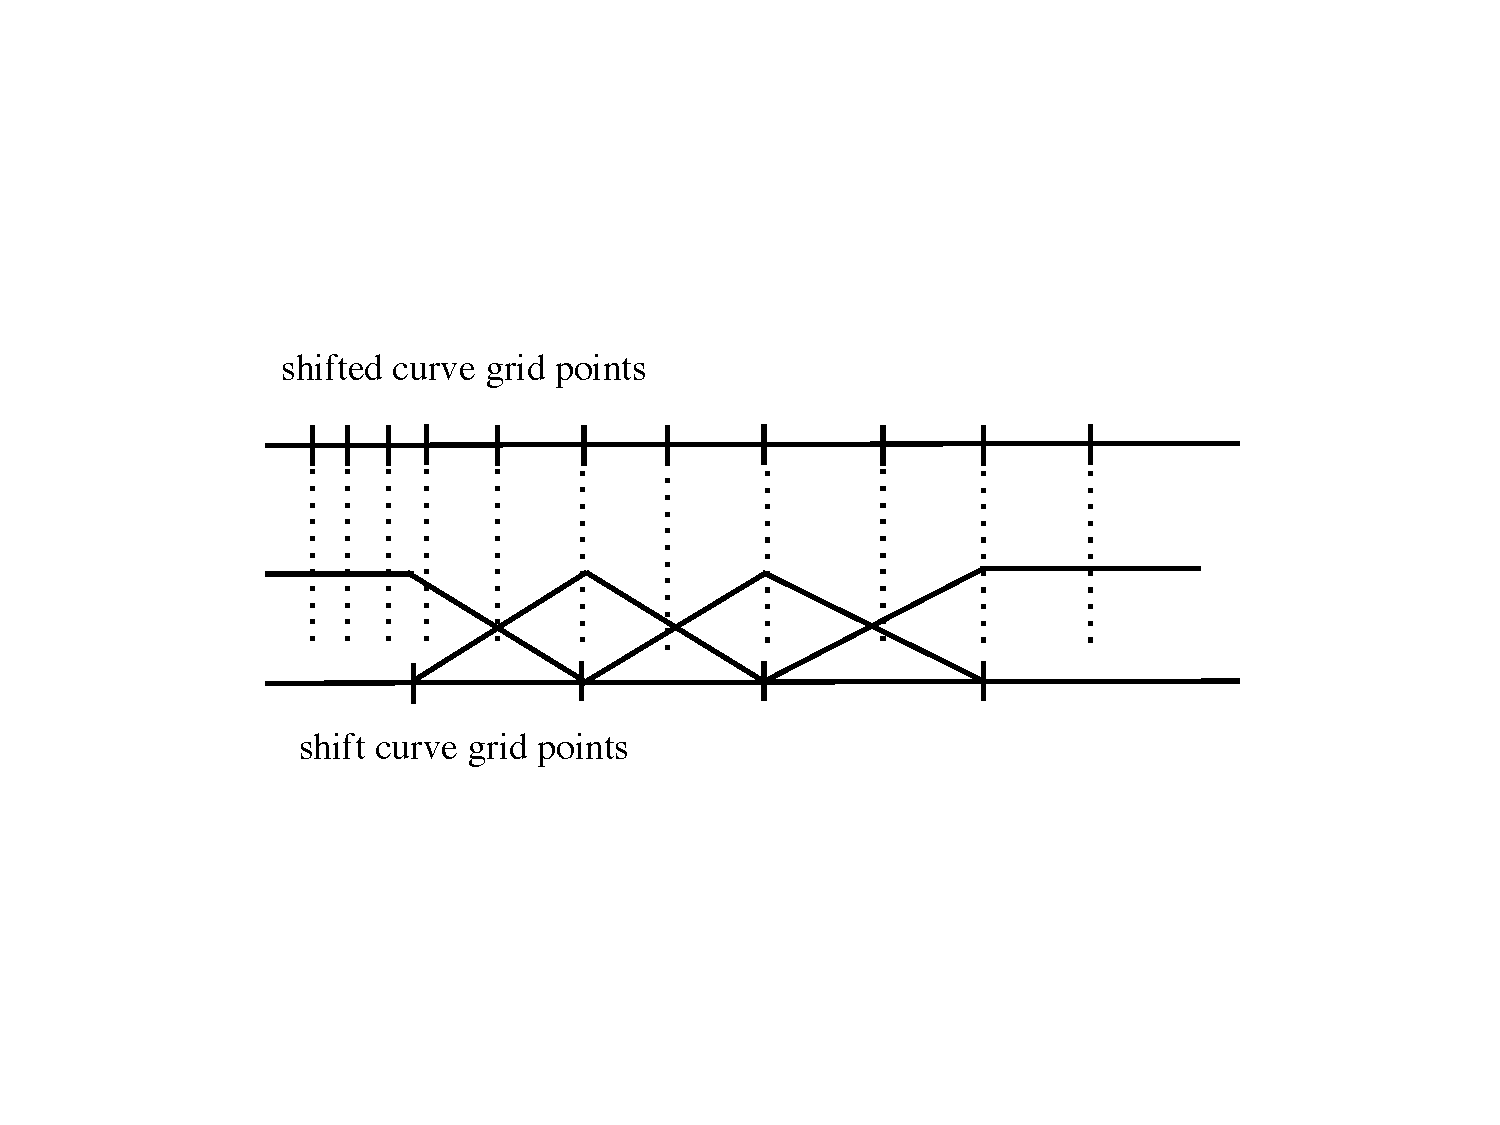
\includegraphics[scale=0.6]{shiftcurve.pdf}
\end{center}
\caption{1-d shift curve (bottom) applied to a more granular underlying curve (top). }
\label{fig_shiftcurve}
\end{figure} 

Shifts at the left and right end of the shift curve are extrapolated flat, i.e. applied to all data of the original curve to the left and to the right of the shift curve ends. In between, all shifts are distributed linearly as indicated to the left and right up to the adjacent shift grid points. As a result, a parallel shift of the all points on the shift curve yields a parallel shift of all points on the underlying curve.   \\

The two-dimensional case is covered in an analogous way, applying flat extrapolation at the boundaries and ``pyramidal-shaped'' linear interpolation for the bulk of the points. 

The details of the computation of sensitivities to implied volatilities in strike direction can be summarised as
follows:

For {\em Swaption Volatilities}, the initial market setup can be an ATM surface only or a full cube. The simulation
market can be set up as ATM only or as a full cube as well, but the latter choice is only possible if a full cube is set
up in the initial market. The sensitivitiy set up must match the simulation setup with regards to the strikes (i.e. it
is ATM only if and only if the simulation setup is ATM only, or it must contain exactly the same strike spreads relative
to ATM as the simulation setup). Finally, if the initial market setup is a full cube, and the simulation / sentivitiy
setup is ATM only, sensitivtiies are computed by shifting the ATM volatility w.r.t. the given shift size and type and
shifting the non-ATM volatilities by the same absolute amount as the ATM volatility.

For {\em Cap/Floor Volatilities}, the initial market setup always contains a set of fixed strikes, i.e. there is no
distinction between ATM only and a full surface. The same holds for the simulation market setup. The sensitivity setup
may contain a different strike grid in this case than the simulation market. Sensitivitiy are computed per expiry and
per strike in every case.

For {\em Equity Volatilities}, the initial market setup can be an ATM curve or a full surface. The simulation market can
be set up as ATM only or a full surface as well, where a full surface is allowed even if the initial market setup in an
ATM curve only. If we have a full surface in the initial market and an ATM curve in the simulation market, sensitivities
are computed as in the case of Swaption Volatilities, i.e. the ATM volatility is shifted w.r.t. the specified shift size
and type and the non-ATM volatilities are shifted by the same absolute amount as the ATM volatility. If the simulation
market contains a full surface, all volatiilties are shifted individually using the specified shift size and type. In
every case the sensitivties are aggregated on the ATM bucket in the sensitivity report.

For {\em FX Volatilities}, the treatment is similar to Equity Volatilities. except for the case of a full surface
definition in the initial market and an ATM only curve in the simulation market. In this case, the pricing in the
simulation market is using the ATM curve only, i.e. the initial market's smile structure is lost.

(For {\em CDS Volatilities} only an ATM curve can be defined.)

In all cases the smile dynamics is ``sticky strike'', i.e. the implied vol used for pricing a deal does not change if
the underlying spot price changes.

\end{appendix}

%========================================================
%\section{References}
%========================================================

\begin{thebibliography}{*}

\bibitem{ORE} \url{http://www.opensourcerisk.org}

\bibitem{QL} \url{http://www.quantlib.org}
 
\bibitem{QRM} \url{http://www.quaternion.com}

\bibitem{quantlib-install} \url{http://quantlib.org/install/vc10.shtml}

%\bibitem{confluence} https://confluence.atlassian.com/bitbucket/set-up-git-744723531.html

\bibitem{git-download} \url{https://git-scm.com/downloads}

\bibitem{boost-binaries} \url{https://sourceforge.net/projects/boost/files/boost-binaries}

\bibitem{boost} \url{http://www.boost.org}

\bibitem{jupyter} \url{http://jupyter.org}

\bibitem{Anaconda} \url{https://docs.continuum.io/anaconda}

\bibitem{LO} \url{http://www.libreoffice.org}

%\bibitem{xlwings} \url{http://www.xlwings.org}

\bibitem{bcbs128} Basel Committee on Banking Supervision, {\em International Convergence of Capital Measurement and
    Capital Standards, A Revised Framework}, \url{http://www.bis.org/publ/bcbs128.pdf}, June 2006

\bibitem{bcbs189} Basel Committee on Banking Supervision, {\em Basel III: A global regulatory framework for more
    resilient banks and banking systems}, \url{http://www.bis.org/publ/bcbs189.pdf}, June 2011

\bibitem{BrigoMercurio} Damiano Brigo and Fabio Mercurio, {\em Interest Rate Models: Theory and Practice, 2nd Edition},
  Springer, 2006.

\bibitem{Pykhtin2010} Michael Pykhtin, {\em Collateralized Credit Exposure}, in Counterparty Credit Risk, (E. Canabarro,
  ed.), Risk Books, 2010

\bibitem{PykhtinRosen} Michael Pykhtin and Dan Rosen, {\em Pricing Counterparty Risk at the Trade Level and CVA
    Allocations}, Finance and Economics Discussion Series, Divisions of Research \& Statistics and Monetary Affairs,
  Federal Reserve Board, Washington, D.C., 2010

\bibitem{Gregory12} Jon Gregory, {\em Counterparty Credit Risk and Credit Value Adjustment, 2nd Ed.}, Wiley Finance,
  2013.

\bibitem{Lichters} Roland Lichters, Roland Stamm, Donal Gallagher, {\em Modern Derivatives Pricing and Credit Exposure
    Analysis, Theory and Practice of CSA and XVA Pricing, Exposure Simulation and Backtesting}, Palgrave Macmillan,
  2015.

\bibitem{Anfuso2016} Fabrizio Anfuso, Daniel Aziz, Paul Giltinan, Klearchos Loukopoulos, {\em A Sound Modelling and
    Backtesting Framework for Forecasting Initial Margin Requirements},
  \url{http://papers.ssrn.com/sol3/papers.cfm?abstract_id=2716279}, 2016

\bibitem{Andersen2016} Leif B. G. Andersen, Michael Pykhtin, Alexander Sokol, {\em Rethinking Margin Period of Risk},
  http://papers.ssrn.com/sol3/papers.cfm?abstract\_id=2719964, 2016

  % \bibitem{SIMM}{SIMM Methodology\\ \tiny
  %   http://www2.isda.org/attachment/ODM1Mw==/ISDA\%20SIMM\%20Methodology\_7\%20April\%202016\_v3.15\%20(PUBLIC).pdf}

  % \bibitem{SIMM_Data_Standards}{SIMM Risk Data Standards\\ \tiny
  %   https://www2.isda.org/attachment/ODQzMg==/Risk\%20Data\%20Standards\_24\%20May\%202016\_v1.22\%20(PUBLIC).pdf}

  % \bibitem{OO} http://www.openoffice.org

\bibitem{LichtersEtAl} Peter Caspers, Paul Giltinan, Paul; Lichters, Roland; Nowaczyk , Nikolai. {\em Forecasting Initial Margin Requirements – A Model Evaluation}, Journal of Risk Management in Financial Institutions, Vol. 10 (2017), No. 4, \url{https://ssrn.com/abstract=2911167}

\end{thebibliography}

\newpage
\addcontentsline{toc}{section}{Todo}
\listoftodos[Todo]
%\todos

\end{document}
